\documentclass[journal abbreviation, manuscript]{copernicus}

\usepackage[utf8]{inputenc}
\usepackage{amsmath, amssymb}
\usepackage{hyperref, float}
\usepackage{booktabs}
\usepackage{pdflscape}
\usepackage{caption, subcaption}
\usepackage{graphicx}
\usepackage{xcolor}

\DeclareMathOperator*{\argmax}{arg\,max}
\DeclareMathOperator*{\argmin}{arg\,min}

\title{Evaluating and Improving the Reliability of Gas-Phase Sensor System Calibrations Across New Locations for Ambient Measurements and Personal Exposure Monitoring}
\date{\today}


\Author[1]{Sharad Vikram}{}
\Author[2]{Ashley Collier-Oxandale}{}
\Author[1]{Michael Ostertag}{}
\Author[1]{Massimiliano Menarini}{}
\Author[1]{Camron Chermak}{}
\Author[2]{Michael Hannigan}{}
\Author[1]{William Griswold}{}

\affil[1]{University of California, San Diego}
\affil[2]{University of Colorado, Boulder}

%% The [] brackets identify the author with the corresponding affiliation. 1, 2, 3, etc. should be inserted.



\runningtitle{TEXT}

\runningauthor{TEXT}

\correspondence{NAME (EMAIL)}



\received{}
\pubdiscuss{} %% only important for two-stage journals
\revised{}
\accepted{}
\published{}

\newcommand\todo[1]{\textcolor{red}{#1}}
\newcommand{\textus}[1]{$_{\text{#1}}$}

\begin{document}

\maketitle

\begin{abstract}

Advances in ambient environmental monitoring technologies are enabling concerned communities and citizens to collect data to better understand their local environment and potential exposures. These mobile, low-cost tools make it possible to collect data with increased temporal and spatial resolution providing data on a large scale with unprecedented levels of detail. This type of data has the potential to empower people to make personal decisions about their exposure and support the development of local strategies for reducing pollution and improving health outcomes.

However, calibration of these low-cost instruments has been a challenge.  Often, a sensor package is calibrated via field calibration. This involves colocating the sensor package with a high-quality reference instrument for an extended period, and then applying machine learning or other model fitting technique such as multiple-linear regression to develop a calibration model for converting raw sensor signals to pollutant concentrations.  Although this method helps to correct for the effects of ambient conditions (e.g., temperature) and cross-sensitivities with non-target pollutants, there is a growing body of evidence that calibration models can overfit to a given location or set of environmental conditions on account of the incidental correlation between pollutant levels and environmental conditions, including diurnal cycles.  As a result, a sensor package trained at a field site may provide less reliable data when moved, or \textit{transferred}, to a different location.  This is a potential concern for applications seeking to perform monitoring away from regulatory monitoring sites, such as personal mobile monitoring or high-resolution monitoring of a neighborhood.  



%. Calibration models commonly overfit to a particular location 

We performed experiments confirming that transferability is indeed a problem and show that it can be improved by collecting data from multiple regulatory sites and building a calibration model that leverages data from a more diverse dataset. We deployed three sensor packages to each of three sites with reference monitors (nine packages total), and then rotated the sensor packages through the sites over time. Two sites were in San Diego, CA, with a third outside of Bakersfield, CA, offering varying environmental conditions, general air quality composition, and pollutant concentrations.  When compared to prior single-site calibration, the multi-site approach exhibits better model transferability for a range of modeling approaches.  Our experiments also reveal that random forest is especially prone to overfitting, and confirms prior results that transfer is a significant source of both bias and standard error.  Bias dominated in our experiments, suggesting that transferability might be easily increased by detecting and correcting for bias.

Also, given that many monitoring applications involve the deployment of many sensor packages based on the same sensing technology, there is an opportunity to leverage the availability of multiple sensors at multiple sites during calibration.  We contribute a new neural network architecture model termed split-NN that splits the model into two-stages, in which the first stage corrects for sensor-to-sensor variation and the second stage uses the combined data of all the sensors to build a model for a single sensor package.  The split-NN modeling approach outperforms multiple linear regression, traditional 2- and 4-layer neural network, and random forest models.


\end{abstract}

\section{Introduction}\label{Introduction}

As the use of low-cost sensor systems for citizen science and community-based research expands, improving the robustness of calibration for low-cost sensors will support these efforts by ensuring more reliable data and enabling a more effective use of the often-limited resources of these groups. These next-generation technologies have the potential to reduce the cost of air quality monitoring instruments by orders of magnitude, enabling the collection of data at higher spatial and temporal resolution, providing new options for both personal exposure monitoring and communities concerned about their air quality. \citep{Snyder2013}.  High resolution data collection is important because air quality can vary on small temporal and spatial scales \citep{Monn1997, Wheeler2008}. This variability can make it difficult to estimate exposure or understand the impact of local sources using data from existing monitoring networks \citep{Wilson2005}, which provide information at a more regional scale. Furthermore, studies have highlighted instances where air quality guidelines have been exceeded on small spatial scales, in so called ‘hot spots’ \citep{Wu2012}. This may be of particular concern for environmental justice communities, where residents are unknowingly exposed to higher concentrations of pollutants due to a lack of proximity to local monitoring stations. One group using low-cost sensors to provide more detailed and locally specific air quality information is the Imperial County Community Air Monitoring Network \citep{English2016}. The goal of this network of particulate monitors is to help inform local action (e.g., keeping kids with asthma inside), or open the door to conversations with regulators \citep{English2016}. In another example, researchers are investigating the potential for wearable monitors to improve personal exposure estimates \citep{Jerrett2017}. 

%While there still exist challenges and limitations, these attributes make low-cost sensing an attractive option for concerned citizens and communities interested in investigating local air quality issues. 

The increasing use of low-cost sensors is driving a growing concern regarding data quality \citep{Clements2017}. Low-cost sensors, particularly those designed to detect gas-phase pollutants, are often cross-sensitive to changing environmental conditions (e.g., temperature, humidity, and barometric pressure) and other pollutant species.  Much work has gone into exploring calibration methods, models, and techniques that incorporate corrections for these cross-sensitives to make accurate measurements in complex ambient environments \citep{Spinelle2014, Spinelle2015, SPINELLE2017706, Cross2017, Sadighi2018, Zimmerman2018}. While the methods of building (or \textit{training}) calibration models differ, these studies have all utilized colocations with high-quality reference instruments in the field, instruments such as Federal Reference Method or Federal Equivalent Method monitors (FRM/FEM) \citep{Spinelle2014, Spinelle2015, SPINELLE2017706, Cross2017, Sadighi2018, Zimmerman2018}. This colocated data allows accurate calibration models to be built for the conditions that the sensors will experience in the field (e.g., diurnal environmental trends and background pollutants). A recurring observation has been that laboratory calibrations, while valuable for characterizing a sensor’s abilities, perform poorly compared to field calibrations likely due to an inability to replicate complex conditions in a chamber \citep{Piedrahita2014, Castell2017}.  

Recently, researchers have begun to explore calibrating sensors in one location and testing them in another, called \textit{transfer}.  Often, a decrease in performance is seen in new locations where conditions are likely to differ from the conditions of calibration.  In one study, researchers testing a field calibration for electrochemical SO\textus{2} sensors from one location in Hawaii and at another location also in Hawaii found a small drop in correlation between the reference and converted sensor data \citep{Hagan2018}. This was attributed to the testing location being a generally less polluted environment \citep{Hagan2018}.  In a study that involved calibration techniques for low-cost metal-oxide O\textus{3} sensors and non-dispersive infrared CO\textus{2} sensors in different environments (e.g., typical urban vs. a rural area impacted by oil and gas activity), researchers found that simpler calibration models (i.e., linear models), although generally lower in accuracy, performed more consistently when faced with significant extrapolations in time or typical pollutant levels and sources\citep{Casey2018testing}. In contrast, more complex models (i.e.,artificial neural networks) only transferred well when there was little extrapolation in time or pollutant sources.  A study utilizing electrochemical CO, NO, NO\textus{2}, and O\textus{3} sensors found that performance varied spatially and temporally according to changing atmospheric composition and meteorological conditions \citep{Castell2017}. This team also found calibration model parameters differed based on where exactly a single sensor node was colocated (i.e., a site on a busy street verses a calm street), supporting the idea that these models are being specialized to the environment where training occurred \citep{Castell2017}.  In a recent study targeting this particular issue with low-cost sensors, electrochemical NO and NO\textus{2} sensors were calibrated at a rural site using multivariate linear regression model, support vector regression models, and a random forest regression model. The performance of these models was then examined at two urban sites (one background urban site and one near-traffic urban site). For both sensor types, random forests were found to be the best-performing models, resulting in mean averages errors between 2–4 ppb and relatively useful information in the new locations \citep{Bigi2018performance}. One important note from the authors is that both sensor signals were included in the models for NO and NO\textus{2} respectively, potentially helping to mitigate cross interference effects \citep{Bigi2018performance}. In another recent study, researchers also compared several different calibration model types, as well as the use of individualized verses generalized models and how model performance is affected when sensors are deployed to a new location \citep{Malings2018Development}.  An individualized model is a model for a sensor based on its own data, whereas a generalized model combines the data from all the sensors of the same type being calibrated. The researchers found that the best-performing and most robust model types varied by sensor type; for example, simpler regression models performed best for electrochemical CO sensors, whereas more complicated models, such as artificial neural networks and random forest models, resulted in the best performance for NO\textus{2}.  Despite the varied results, in terms of the best performing model types, the researchers observed that across the different sensor types tested, generalized models resulted in more consistent performance at new sites than individualized models despite having slightly poorer performance during the initial calibration \citep{Malings2018Development}.  If this observation holds across sensor types and the use in other locations, it could help solve the problem of scaling up sensor networks allowing for much larger deployments. 

The mixed results and varying experimental conditions of these studies highlight the need for a more comprehensive understanding of how and why calibration performance degrades when sensors are moved. A better understanding could inform potential strategies to mitigate these effects.  As recent research has successfully applied advanced machine learning techniques to improve sensor calibration models \citep{Zimmerman2018, DeVito2009, Casey2018Performance}, we believe these techniques could also be leveraged in innovative ways to improve the transferability of calibration models.

This paper contributes an extensive transferability study as well as new techniques for data collection and model construction to improve transferability.  We hypothesize that transferability is a real issue for sensors that exhibit cross-sensitivities.   Based on the hypothesis that the increased errors under transfer are due to overfitting, we propose that training a calibration model on multiple sites will improve transfer.  Finally, based on the hypothesis that more data is generally better in field calibration, we propose that transfer can be further improved with a new modeling method (split-NN) that can use the data from multiple sensor packages to train a single sensor's model.

%...by widening the distribution of the training data

As many previous studies studied colocation with reference measurements in one location and a validation at a second location, we designed a deployment that included triplicates of sensor packages colocated at three different reference monitoring stations and then rotated through the three sites – two  near the city of San Diego, CA and one in a rural area outside of Bakersfield, CA.   This allows for further isolating the variable of a new deployment location. The analysis focuses on data from electrochemical O\textus{3} and NO\textus{2} sensors, although other sensor types were deployed and used in the calibration, analogous to \citep{Bigi2018performance}.  These pollutants are often of interest to individuals and communities given the dangers associated with ozone exposure \citep{Brunekreef2002Air}, and nitrogen dioxide’s role in ozone formation. In studying these pollutants, we are adding to the existing literature by examining the transferability issue in relation to electrochemical O\textus{3} and NO\textus{2} sensors, which are known to exhibit cross-sensitive effects \citep{SPINELLE2015480}.  We compare the transferability of multiple linear regression models, neural networks, and random forest models.  Based on these measurements and comparisons, we contribute the following results:

\begin{itemize}
\item Our experiments confirm that calibration model error increases when the model is transferred to a new location.  This holds over all the modeling methods we tested.
\item Much of the error under transfer was bias error.  Given the simple structure of bias error, this suggests that transferability might be easily increased by detecting and correcting for bias.
\item Although random forest methods perform extremely well when trained and tested at a single site, its advantages are largely lost under transfer.
\item Training a calibration model on multiple sites improves transferability.
\item Finally, for applications involving the deployment of many sensor packages based on the same sensing technology, we show it is possible to improve transferability by exploiting the presence of multiple sensors at multiple sites during field calibration.  We contribute a new model training method via a two-stage "split" neural network.  The first stage corrects for deviations in sensor performance (essentially bias) and the second stage combines all the data of all the sensors to build a model for a single sensor package.  This modeling approach outperforms other approaches.
\end{itemize}
 
%Using this data set, we explore (1) how well different calibration techniques hold up across new environments, (2) what is causing a drop in performance in new locations, (3) and solutions and recommendations for sensor users to ensure the most robust calibration possible. 

\section{Methods}

\subsection{Sampling Sites}\label{SamplingSites}

\begin{figure}
\centering
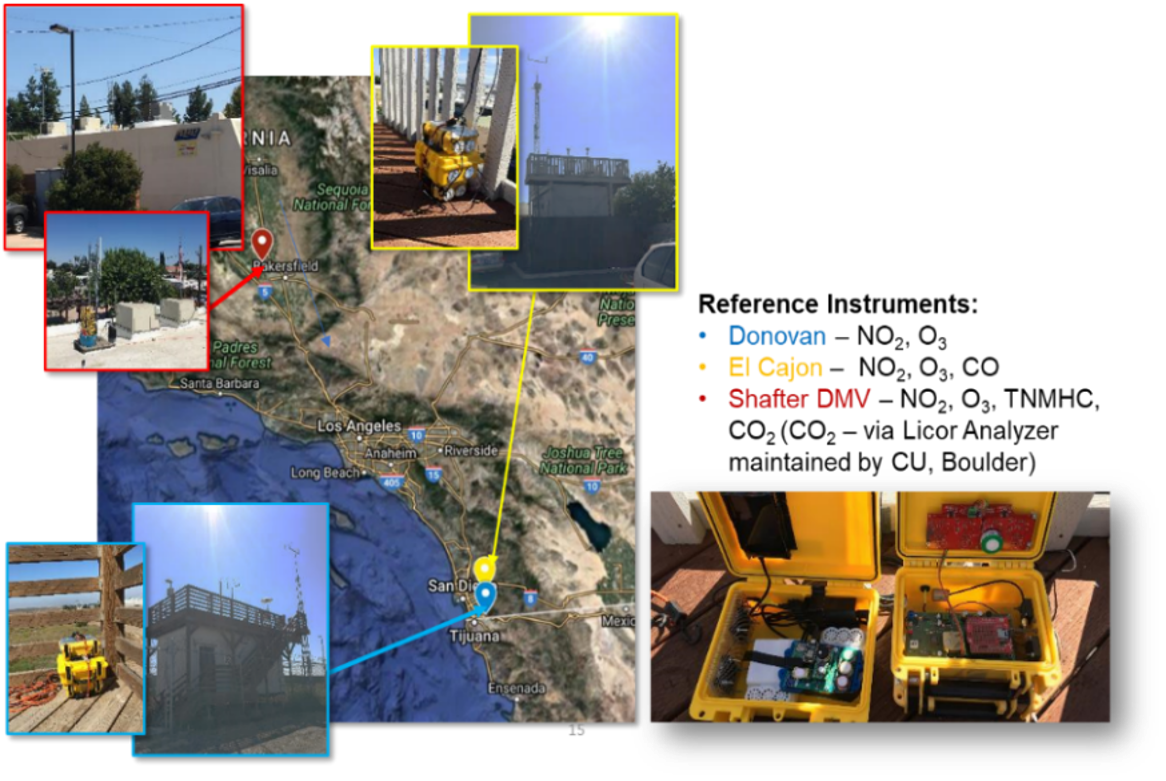
\includegraphics[width=0.75\textwidth]{writeup/img/MSdeployment.png}
\caption{Map and images of deployment locations. Shafter DMV (red) was located 250 mi away from Donovan (blue) and El Cajon (yellow), which were located in San Diego, CA. (bottom right) Deployment containers configuration for the extended deployment. Each container has active ventilation to keep the internal conditions equivalent to the ambient environment.}
\label{fig:img-map}
\end{figure}

For this deployment, we coordinated with three regulatory monitoring sites and rotated sensor packages through each site over the course of approximately six months. Each monitoring site included reference instruments for NO\textus{2} and O\textus{3}, among others. The first site was in El Cajon, CA, in a suburban area east of San Diego, CA near an elementary school and a major highway (El Cajon Site). The second site was directly south 15 miles in the south east corner of San Diego, a more rural area approximately two miles from the border crossing for heavy duty vehicles at Otay Mesa (Donovan Site). The third site was in rural Shafter, CA, 250 miles to the north near Bakersfield.  It is considerably inland compared to the other sites with nearby agriculture as well as oil and gas extraction activities. We expected to see a unique environmental profile (i.e., temperature, humidity, and barometric pressure) at the Shafter site due to being considerably more inland, where weather would be more dominated by the desert ecosystem rather than the ocean ecosystem.  We also expected to see unique emission profiles among the sites.  Donovan was expected to show higher truck emissions due to the presence of heavy duty vehicles, potentially idling for long periods of time, while Shafter was expected to be affected by emissions from its nearby oil and gas activity. We expected the El Cajon site's emissions profile to resemble that of a typical urban/suburban site.  This variety of environmental and emissions profiles would allow us to meaningfully test for transferability, in particular to assess to what degree a calibration model trained on one site would overfit for the other sites.

\subsection{The MetaSense System}

\subsubsection{Hardware Platform}

A low-cost air quality sensing platform was developed to interface with commercially available sensors, initially described in \citet{Chan2017context}. The platform was designed to be mobile, modular, and extensible, enabling end users to configure the platform with sensors suited to their monitoring needs. It interfaces with the Particle Photon or Particle Electron platforms, which contain a 24 MHz ARM Cortex M3 microprocessor and a Wi-Fi or 3G cellular module, respectively. In addition, a Bluetooth Low Energy (BLE) module supports energy efficient communication with smartphones and other hubs with BLE connectivity. The platform can interface with any sensor that communicates using standard communication protocols (i.e. analog, I2C, SPI, UART) and supports an input voltage of 3.3 V or 5.0 V. The platform can communicate results to nearby devices using BLE or directly to the cloud using Wi-Fi or 2G/3G cellular, depending on requirements.  USB is also provided for purposes of debugging, charging, and flashing the firmware.  The firmware can also be flashed or configured over the air. An SD card slot provides the option for storing measurements locally, allowing for completely disconnected and low-power operation.

Our configuration utilized electrochemical sensors for traditional air quality indicators (NO\textus{2}, CO, O\textus{3}), nondispersive infrared sensors for CO\textus{2}, photoionization detectors for volatile organic compounds (VOCs), and a variety of environmental sensors (temperature, humidity, barometric pressure). The electrochemical sensors (NO\textus{2}: Alphasense NO\textus{2}-A43F, O\textus{3}: Alphasense O\textus{3}-A431, and CO: Alphasense CO-A4) are mounted to a companion analog front end (AFE) from Alphasense, which assists with voltage regulation and signal amplification. Each sensing element has two electrodes which give analog outputs for the working electrode (WE) and auxiliary electrodes (AE). The difference in signals is approximately linear with respect to the ambient target gas concentration but have dependencies with temperature, humidity, barometric pressure, and cross-sensitivities with other gases. The electrochemical sensors generate an analog output voltage, which is connected to a pair of analog-to-digital converters (ADCs), specifically the TI ADS1115, and converted into a digital representation of the measured voltage, which is later used as inputs for our machine learning models.

% Electrochemical sensors offer a relatively high level of accuracy at a low current consumption. 

\begin{figure}
\centering
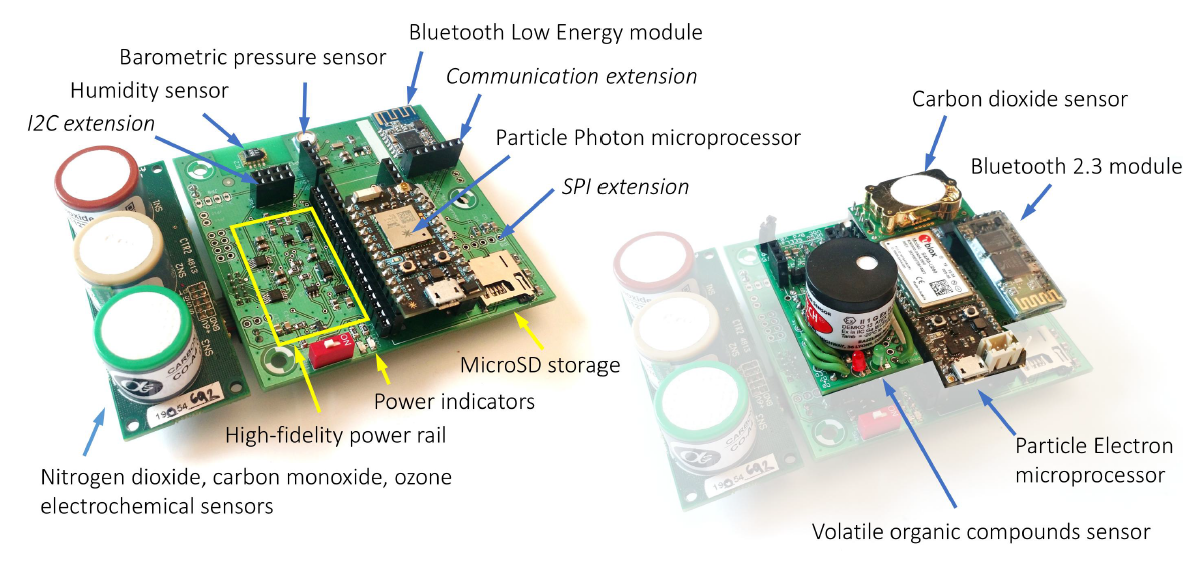
\includegraphics[width=0.75\textwidth]{writeup/img/metasense-platform}
\caption{Labeled MetaSense Air Quality Sensing Platform. (Left) Modular, extensible platform in standard configuration with NO\textus{2}, O\textus{3}, and CO electrochemical sensors. (Right) Additional modules that can be added to the board for additional measurement capabilities.}
\label{fig:img-label}
\end{figure}

Modern low-cost electrochemical sensors offer a low cost and low power method to measure pollutants, but currently available sensors are more optimized for industrial applications than air pollution monitoring: the overall sensing range is too wide and the noise levels are too high. For example, the AlphaSense A4 sensors for NO\textus{2}, O\textus{3}, and CO have a measurement range of 20, 20, and 500 ppm, respectively, which is significantly higher than the unhealthy range proposed by the United States Air Quality Index. Unhealthy levels for NO\textus{2} at 1-hour exposure range from 0.36 – 0.65 ppm, O\textus{3} at 1-hour exposure from 0.17 – 0.20 ppm, and CO at 8-hour exposure from 12.5 – 15.4 ppm (Uniform Air Quality Index (AQI) and Daily Reporting, ~\citeyear{AQI2015}). Along with the high range, the noise levels of the sensors make it difficult to distinguish whether air quality is good. Using the analog front end (AFE) offered by Alphasense, the noise levels for NO\textus{2}, O\textus{3}, and CO have standard deviations of 7.5 ppb, 7.5 ppb, and 10 ppb, respectively. These standard deviations are large compared to observed signal levels for NO\textus{2} and O\textus{3} measurements, which ranged between 0 – 35 ppb and 12 – 60 ppb, respectively, during the 6 month testing period.

The ambient environmental sensors accurately measure temperature, humidity, and pressure and are important for correcting the environmentally related offset in electrochemical sensor readings. The TE Connectivity MS5540C is a barometric pressure sensor capable of measuring across a 10 to 1100 mbar range with 0.1 mbar resolution. Across 0 C to 50 C, the sensor is accurate to within 1 mbar and has a typical drift of +/- 1 mbar per year. The Sensiron SHT11 is a relative humidity sensor capable of measuring across the full range of relative humidity (0 to 100\% RH) with a 0.05\% RH resolution. Both sensors come equipped with temperature sensors with $\pm$0.8 C and $\pm$0.4 C accuracy, respectively. The sensors stabilize to environmental changes in under 30 seconds, which is sufficiently fast to accurately capture changes in the local environment.

In order to improve the robustness of the boards to ambient conditions, the electronics were conformally coated with silicone and placed into an enclosure as shown in Figure~\ref{fig:img-enclosure}. The housing prevents direct contact with the sensors by providing ports over the electrochemical sensors and a vent near the ambient environmental sensors. The system relies on passive diffusion of pollutants into the sensors due to the high power cost of active ventilation.  However, as described in Section~\ref{DataCollection}, for this study the housed sensor packages were placed in an actively ventilated container.

%The passive diffusion model is acceptable for the mobile sensor use case, though, because external movement of the sensor will cause a higher exchange rate of air into the enclosure. 
%WGG: I think it may not be entirely acceptable. :)


\begin{figure}[t]
\centering
\includegraphics[width=0.75\textwidth]{writeup/img/MetaSense_enclosure_outline.png}
\caption{An enclosure was 3D printed for the MetaSense Air Quality Sensing Platform with top-side ports above the electrochemical sensors and a side port next to the ambient environmental sensors.}
\label{fig:img-enclosure}
\end{figure}

\subsubsection{Software Infrastructure}

%We developed the software infrastructure for the MetaSense sensing platform to support multiple usage scenarios. The firmware is configured to support four communication media. A board can communicate via Bluetooth Low Energy (BLE) or USB to a control program that can configure the platform and collect real-time data. The USB connection also supports debugging the board, charging the board, and updating the firmware. Depending on the hardware configuration, Photon or Electron, the MetaSense board can connect directly to the cloud via Wi-Fi or 3G cellular, respectively. These mediums enable over-the-air firmware updates. Each sensor is equipped with an SD card, allowing all readings to be stored locally for redundancy and for deployment situations where energy consumption is critical.

We developed two applications for Android smartphones that leverage the BLE connection of the MetaSense platform. The first application, the MetaSense Configurator app, enables users to configure the hardware for particular deployment scenarios, adjusting aspects such as sensing frequency, power gating of specific sensors connected, and the communication networks utilized.  The second application, simply called the MetaSense app, collects data from the sensor via BLE and uploads all readings to a remote database.  Each sensor reading is stamped with time and location information, supporting data analysis for mobile use cases. Moreover, users can read the current air quality information on their device, giving them immediate and personalized insight into their exposure to pollutants.

% For example, CO\textus{2} and VOC sensor readings can be enabled or disabled by the configuration application. In another example, if the MetaSense sensing platform is being used as a mobile sensor tethered to a smartphone over BLE, users can disable Wi-Fi (or Cellular) radios to save power. 

The remote measurements database is supported by the MetaSense cloud application and built on Amazon's AWS cloud.  Not only can the MetaSense app connect to this cloud, but the MetaSense boards can be configured to connect directly to it using Wi-Fi or 3G.  The measurement data can be processed by machine learning algorithms in virtual machines in AWS or the data can be downloaded to be analyzed offline.  The aforementioned over-the-air firmware updates are handled through Particle's cloud, which also allows remotely monitoring, configuring and resetting boards. These direct-to-cloud features are key to supporting a long-term, wide-scale deployment like the one presented in this paper.

\subsection{Data Collection and Preprocessing}
\label{DataCollection}
To support a long-term deployment in potentially harsh conditions, the sensors were placed into environmentally robust containers, shown in Figure~\ref{fig:img-map}, bottom right. The container was a dry box, measuring 27.4 x 25.1 x 12.4 cm, that was machined to have two sets of two vents on opposing walls. Louvers were installed with two 5 V, 50 mm square axial fans expelling ambient air from one wall and two louvers allowing air to enter the opposite side. The configuration allowed the robust container to equilibrate with the local environment for accurate measurement.  Each container could hold up to three MetaSense boards with cases and complementary hardware.  Due to the long timeframe of the deployment, a USB charging hub was installed into the container to power the fans, the air quality sensors, and either a BLU Android phone or Wi-Fi cellular hotspot. The phones and hot spots were used to connect the sensors to the cloud; therefore, we could remotely monitor the sensors’ status in real-time and perform preliminary data analysis and storage. Each board also had an SD card to record all measurements locally, increasing the reliability of data storage. 

Each container holding three MetaSense sensor packages was placed at one of three sites for simultaneous data collection across the sites. After a period of time the containers were rotated to a new site such that every package spent a period of time at every site.  We performed three rotations such that every sensor was returned to its original site for the final collection, but we disregarded the data from the initial round 0, except to verify that sensor performance had not changed measurably between the beginning and the end of the deployments. \autoref{tab:board-rotations} lists the dates for each rotation as well as where each sensor system was located for each rotation.  The dates are approximate due to the logistics of gaining access to regulatory field sites and the distances traveled to deploy sensors.  Also of note is that the deployments are not of equal length.  This does not affect the results reported below because we ran all combinations of training and testing sites, and training set sizes were normalized to remove the influence of training set size. The data from the reference monitors was provided by the cooperating air quality districts in the form of minute-averaged O\textus{3} and NO\textus{2} concentrations for the time period that our sensor packages were deployed.

\begin{table}[t]
\centering
\caption{Board locations and dates for each round.}
\begin{tabular}{l|llll}
                  & \textbf{Round 1} &            \textbf{Round 2} &                   \textbf{Round 3} \\
         & \textbf{9/26/17 - 10/19/17} & \textbf{10/19/17 - 12/21/17} & \textbf{12/21/17 - 3/5/18} \\ \hline
\textbf{Board 17} & El Cajon    & Shafter      & Donovan    \\
\textbf{Board 19} &  El Cajon    & Shafter     & Donovan   \\
\textbf{Board 21} &  El Cajon    & Shafter     & Donovan  \\ \hline
\textbf{Board 11} &  Shafter      & Donovan  & El Cajon  \\
\textbf{Board 12} &  Shafter      & Donovan  & El Cajon  \\
\textbf{Board 13} &  Shafter      & Donovan  & El Cajon  \\ \hline
\textbf{Board 15} &  Donovan   & El Cajon   & Shafter    \\
\textbf{Board 18} &  Donovan   & El Cajon   & Shafter     \\
\textbf{Board 20} &  Donovan   & El Cajon   & Shafter   
\end{tabular}
\label{tab:board-rotations}
\end{table}

Prior to using the dataset for training the calibration models, we performed a preprocessing step. First, we programmatically filtered out data samples that contained anomalous values that might have occurred due to a temporary sensor board malfunction (e.g., due to condensation).  Specifically, we searched for temperature and voltage spikes that were outside the realm of reasonable values (i.e., temperature values above 60 degrees Celsius or ADC readings above 5 volts) and removed the corresponding measurements.  Each removed sample was visually inspected to ensure data was not being erroneously removed. The remaining data was averaged over a minute window to match the time resolution of the data from the reference monitors.  Although we gathered sensor voltage measurements from both the auxilliary ($AE$) and working electrodes ($WE$) of the electrochemical sensors, we used the difference between the two ($AE - WE$) as the representative voltage for each sensor since the auxilliary voltage is meant to serve as a reference voltage for the working electrode. This treatment is consistent with the methodology of \citet{Zimmerman2018}, and we validated that the performance of the calibration models did not differ between tests with both electrodes and test with the difference as input features. The resulting data set over the three rounds at the three site contains 1,200,000 minute-averaged measurements.

With this data, we were able to verify our claim in Section \ref{SamplingSites} that we would observe varied environmental and pollutant conditions among the sites. Generally higher ozone values were reported at Shafter, whereas generally higher NO\textus{2} values were reported at Donovan.  Higher humidity values were reported at the Donovan and El Cajon sites, as compared to Shafter.  Some of the lowest temperature values were reported at Shafter.  For more information see the distribution plots in Appendix \ref{Distributions}. 

\subsection{Baseline Calibration Methods}\label{sec:calibration-methods}
Sensor calibration is the process of developing and training models to convert a sensor voltage into a pollutant concentration. We formulate sensor calibration as a regression problem with input features $x$ and $e$ representing signals from the electrochemical sensors (O\textus{3} voltage, NO\textus{2} voltage, CO voltage) and environmental factors (temperature, pressure, humidity), respectively, for a total of 6 features. These features are input to a calibration function $h_\theta(x, e)$ that estimates target values $y$ representing pollutant concentrations (O\textus{3} ppb and NO\textus{2} ppb). 

In our regression problem, we seek a function such that $h_\theta(x, e) \approx y$, which we formulate as an optimization where we minimize error over a training data set $\{x_n, e_n, y_n\}_{n = 1}^N$ according to a loss function $L(h_\theta(x, e), y)$, i.e. 
\begin{equation}
\theta^* = \argmin_\theta \frac{1}{N}\sum_{n = 1}^N L(h_\theta(x_n, e_n), y_n)
\end{equation}
Models trained in this way assume that at inference time, predictions are made on data sampled from the training distribution. While this assumption holds true when the air quality sensors are trained and tested at the same site, the distribution of pollutants and environmental conditions changes when the sensors are moved to a new location. 

We investigated the performance of three calibration models: multiple linear regression, neural networks (sometimes called deep learning), and random forest.  These methods vary in their ability to accurately model complex behaviors, otherwise known as \textit{capacity}, with linear regression having relatively low capacity and neural nets and random forests having substantial capacity.  The price of high capacity is the potential to overfit the training distribution, which is a failure to generalize beyond the training data. Models that overfit will incur significant error when predicting on out-of-distribution examples. Overfitting can be mitigated with regularization and by reducing the model capacity, but this can only go so far if the testing distribution is substantially different from the train distribution. All of these methods have been previously applied to ambient pollutant estimation by various research groups \citep{Piedrahita2014,Spinelle2015,SPINELLE2017706,Sadighi2018,Zimmerman2018,Casey2018testing} and are generally common predictive modeling methods.  For neural nets, we investigated three variants: two-layer, four-layer, and four-layer with a "split" architecture, which we motivate and describe in the next subsection.

%The MetaSense project is concerned with deploying mobile, portable sensors and thus we wish to train calibration models that can generalize beyond the data obtained via colocation. As previously described, we colocated MetaSense boards with EPA stations across three locations in California (El Cajon, Donovan, Shafter). By training a calibration model on training data restricted to some sites and testing on the other site, we measure how well particular models generalize to different locations.

Our baseline models were trained using the Scikit-Learn Python package, and the model parameters for each baseline model can be seen below:
\begin{enumerate}
    \item \textbf{Linear regression:} we assume the functional form $h(x) \triangleq w^T x + b$, and fit the parameters in closed form. We use no regularization or polynomial features.
    \item \textbf{Two-layer neural network:} we fit a two-hidden layer (200 wide) multilayer perceptron with rectified-linear unit activation functions and a final linear layer. We train this neural network using the Adam optimizer ($\beta_0 = 0.9, \beta_1 = 0.999$) and a learning rate of $10^{-3}$.
    \item \textbf{Four-layer neural network:} Same as two-layer neural network, but four hidden layers of width 200 instead of two.
    \item \textbf{Random forest:} We divide our data into five folds and train a random forest of size 100 on each fold, resulting in 500 trees. We aim to reproduce the strategy of \cite{Zimmerman2018} as closely as possible.
\end{enumerate}

\iffalse
\begin{align*}
    \mathrm{MAE}(h(x), y) &= |h(x) - y| \\
    \mathrm{CvMAE}(h(x), y) &= \frac{1}{\textrm{Average conc. of pollutant}}|h(x) - y| \\
\end{align*}
\fi

\subsection{Split Neural Network Method}\label{sec:split-nn}
Overfitting is a problem for high capacity models with a limited distribution in training data, resulting in poor performance when a model is transferred to new locations and environments. One method to improve model transferability would be to collect more training data that includes the test distribution. However, colocating a sensor at multiple different regulatory field sites in order to capture a sufficiently wide distribution is prohibitive in terms of cost and time.  An alternative solution is to deploy a set of sensors based on the same technology across multiple sites and then pool their data.  However, there can be substantial sensor-to-sensor variance in performance that would amplify prediction errors.  We propose a training architecture that consists of two sets of models: a global calibration model that leverages the data from a set of similar sensors spread across different training environments and sensor-specific calibration models that detect and correct the error between sensors.

In the previous subsection, we associated each board $i$ with a calibration function $h_{\theta_i}(x)$ and fit this calibration function with its colocated data. Now, consider a collection of many air quality sensors. We propose using a calibration function split into two distinct steps: first, pollutant sensor voltages $x$ are input into a sensor-specific model, $s_{\theta_i}(x)$, a function parameterized by $\theta_i$, which outputs a fixed dimensional vector $u$~\citep{Goodfellow-et-al-2016}. This intermediate representation $u$ is concatenated with environmental data $e$, which is then passed into a global calibration model $c_\phi([u | e])$. For a single air quality sensor, our final calibration function is $c_\phi([s_{\theta_i}(x) | e])$.  Figure~\ref{fig:split-nn-deploy} depicts the use of such a model.  Such a model is called a split neural network model (\textit{split-NN}) since neural networks are generally used for both the sensor-specific models and the global calibration models. In our experiments, the sensor-specific model $s_{\theta_i}$ is either a linear regressor or neural network  and $c_\phi$ is a two-layer, 100-wide neural network. 

The purpose of the split-NN model is that $s_{\theta_i}$ corrects for differences in air quality sensor $i$'s performance relative to the other sensors, thus normalizing the values and making the behavior of all the sensors compatible with the global model $c_\phi$.  The performance of the estimates from $c_\phi$ should be superior to those from an individual sensor model because it been trained on the (normalized) data of all the boards as opposed to just a single board.

\begin{figure}
    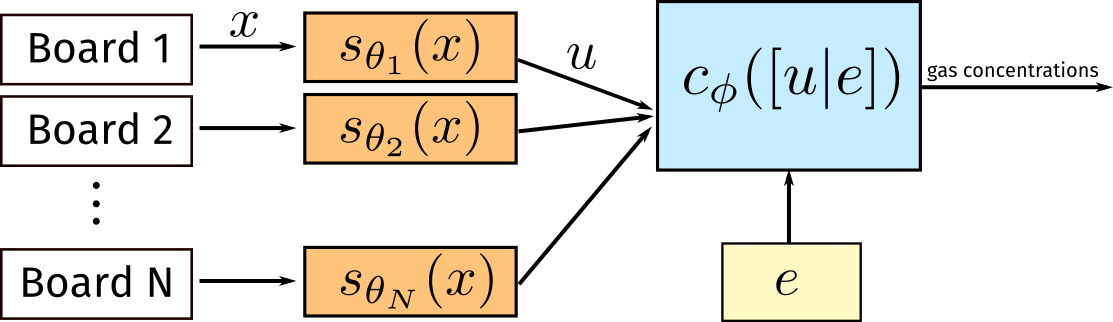
\includegraphics[width=0.8\textwidth]{writeup/img/split-model.png}
    \caption{Architecture of the split-NN model in deployment (testing).  Each air quality sensor has its own custom $s_{\theta_i}(x)$ that is intended to take the sensor's output ($x$) and normalize it ($u$) relative to the other sensors, so that it can be fed into the global model $c_\phi$.}
    \label{fig:split-nn-deploy}
    \todo{WGG: not clear that Board 2 - Board N should be in this figure.  Maybe grayed out?  No additional subscripts needed.}
\end{figure}

The split model can be trained efficiently with stochastic gradient descent. Specifically, we first collect $N$ data sets for each board $D_i = \{x^{(i)}, e^{(i)}, y^{(i)}\}_{i = 1}^N$. We ensure each of these data sets is the same size by sampling each with replacement to artificially match the largest data set. We then pool the data sets together into one data set from which we sample mini-batches. While each sensor-specific model $s_{\theta_i}$ is trained only on data collected by its sensor, the regression with the other $s_{\theta_i}$ sensor-specific models is designed to detect and correct its bias, outputting an intermediate representations $u$ that is normalized with the others.  The global calibration model is trained on the normalized data from all air quality sensors.

%\todo{WGG: word choice on the above: optimization, NN loss function contains loss terms from every single board, the optimal performance will happen when they report the same things when they measure the same things} 

Although training this neural network will take longer than training one for a single board, it has several key advantages over conventional calibration techniques. The first is its ability to share information across multiple boards. Suppose Board A is trained on Location 1 and Board B is trained on Location 2. Pooling the data sets and using a shared model enables the global calibration model to predict well in both locations, and the calibration models for both boards will have information about the other locations in them, in theory improving transferability. The second is more efficient utilization of data. By pooling data and training jointly, we effectively multiply our data size by the number of boards.  Alternatively, field deployments can be shortened.

\textbf{Calibrating a New Board without a Full Training.}  Field calibration is traditionally performed by colocating a sensor package with reference monitors and then training to match pollutant concentrations.  But, suppose we already had a fleet of low-cost sensor packages already deployed.  A simpler method not requiring coordination with regulatory agencies would be to colocate it with a calibrated sensor package and train a model to match its predicted pollutant levels. This risks compounding errors across models, however. 

The split-NN model enables calibrating a new sensor package by colocating to match \textit{representation} instead of predictions~\citep{Goodfellow-et-al-2016}.  We propose calibrating sensor package $N+1$ to match the intermediate representation output of a colocated, previously-calibrated sensor package. Specifically, we train model $N + 1$ to minimize $L(u_N, u_{N + 1})$, or the loss between the two packages' intermediary outputs. These intermediate representations are designed to be robust to changes in location so training to match these representation so it is expected that it will result in a robust calibration model. We analyze this potential calibration technique by holding out a board from our data sets and training a split model. We then simulate calibrating the held out board by training a sensor model to match the representations produced by another board it was colocated with. We then use this new sensor model with the global calibration function to produce pollutant values. 

%The split-NN offers a novel method to calibrate new boards. Suppose we have a set of $N$ calibrated boards and are presented with an uncalibrated $N + 1$-th board. The safest way to calibrate this new board would is always to colocate it with a ground-truth sensor and train a model.  This requirement, however, is potentially restrictive and expensive, as it necessitates deploying the sensor by an EPA or other reliable sensor. On the other hand, colocating with another low cost sensor is simple and cheap, but risks compounding the noise and error that already exist.

\section{Results and Discussion}

\subsection{Robustness of Different Calibration Techniques Across New Locations}
We evaluated a set of four baseline models described in Section~\ref{sec:calibration-methods}: multiple linear regression, two-layer neural network (NN-2), four-layer neural network (NN-4), and random forest (RF). With each of these four models, we performed a suite of identical calibration benchmarks that measure the robustness of models to out-of-distribution data. We split all data sets uniformly at random into training and testing subsets, reserving 20\% of each board's data for testing.  In each benchmark, we progressively widened the training distribution by combining training data from more locations (using subsampling to maintain the training set size), while keeping the testing set data set from one location.  We have four ``levels'' of such benchmarks:
\begin{itemize}
    \item \textbf{Level 0:} Train a model on one location and test on the same location.  Several studies, discussed in Section \ref{Introduction}, have previously assessed this configuration \citep{Zimmerman2018,Spinelle2015,SPINELLE2017706,Cross2017}.
    \item \textbf{Level 1:} Train a model on one location and test on another location.  Some recent studies, also discussed in Section \ref{Introduction}, have previously studied this configuration \citep{Hagan2018, Casey2018testing, Bigi2018performance, Malings2018Development}.
    \item \textbf{Level 2:} Train a model on two locations and test on a third location.
    \item \textbf{Level 3:} Train a model on three locations and test on one of the three locations.
\end{itemize}
\begin{figure}
\begin{subfigure}{0.23\textwidth}
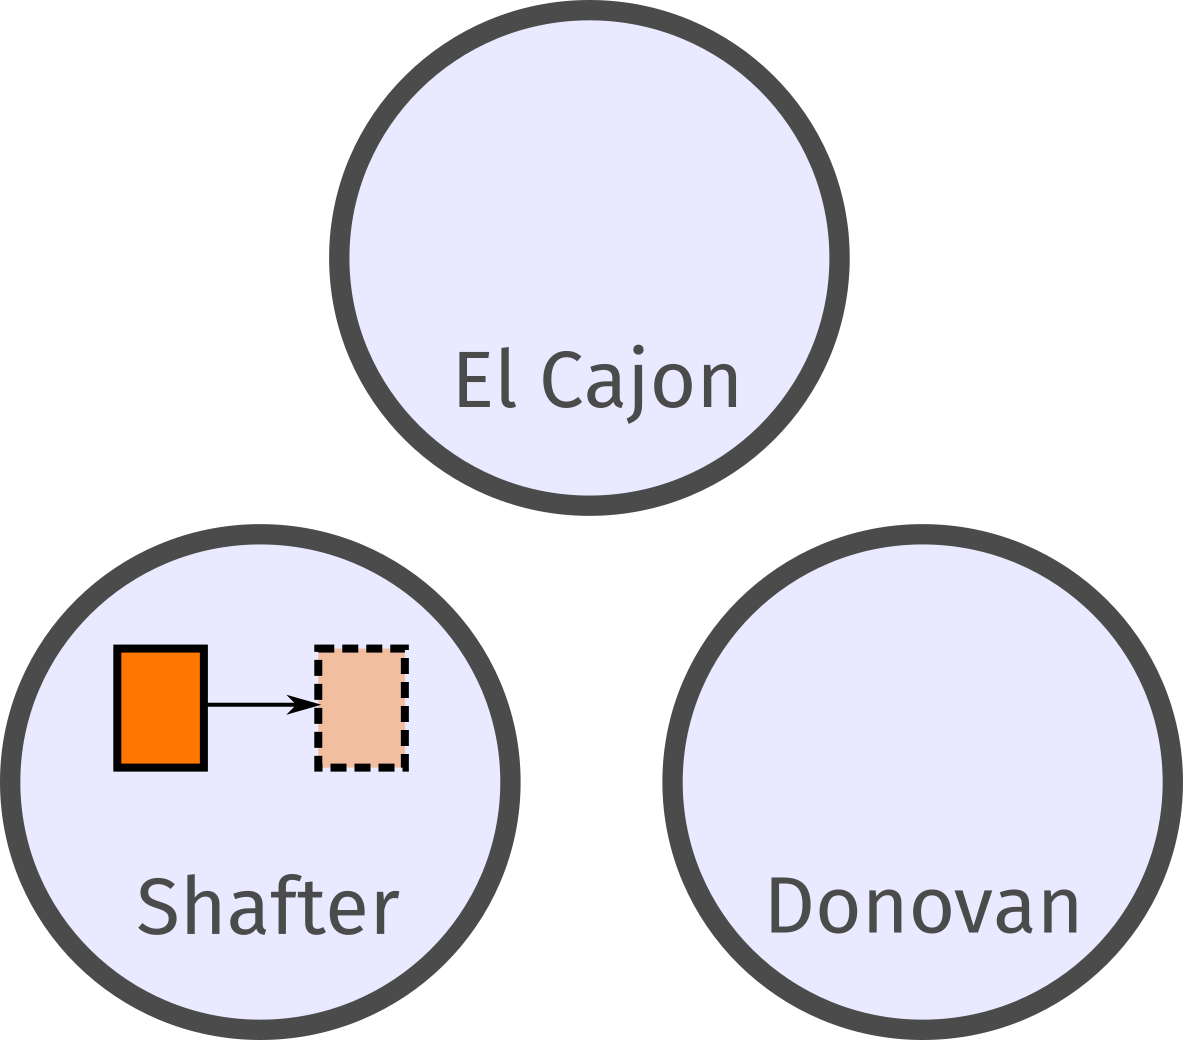
\includegraphics[width=\textwidth]{writeup/img/level0.png}
\caption{Level 0}
\end{subfigure}
~
\begin{subfigure}{0.23\textwidth}
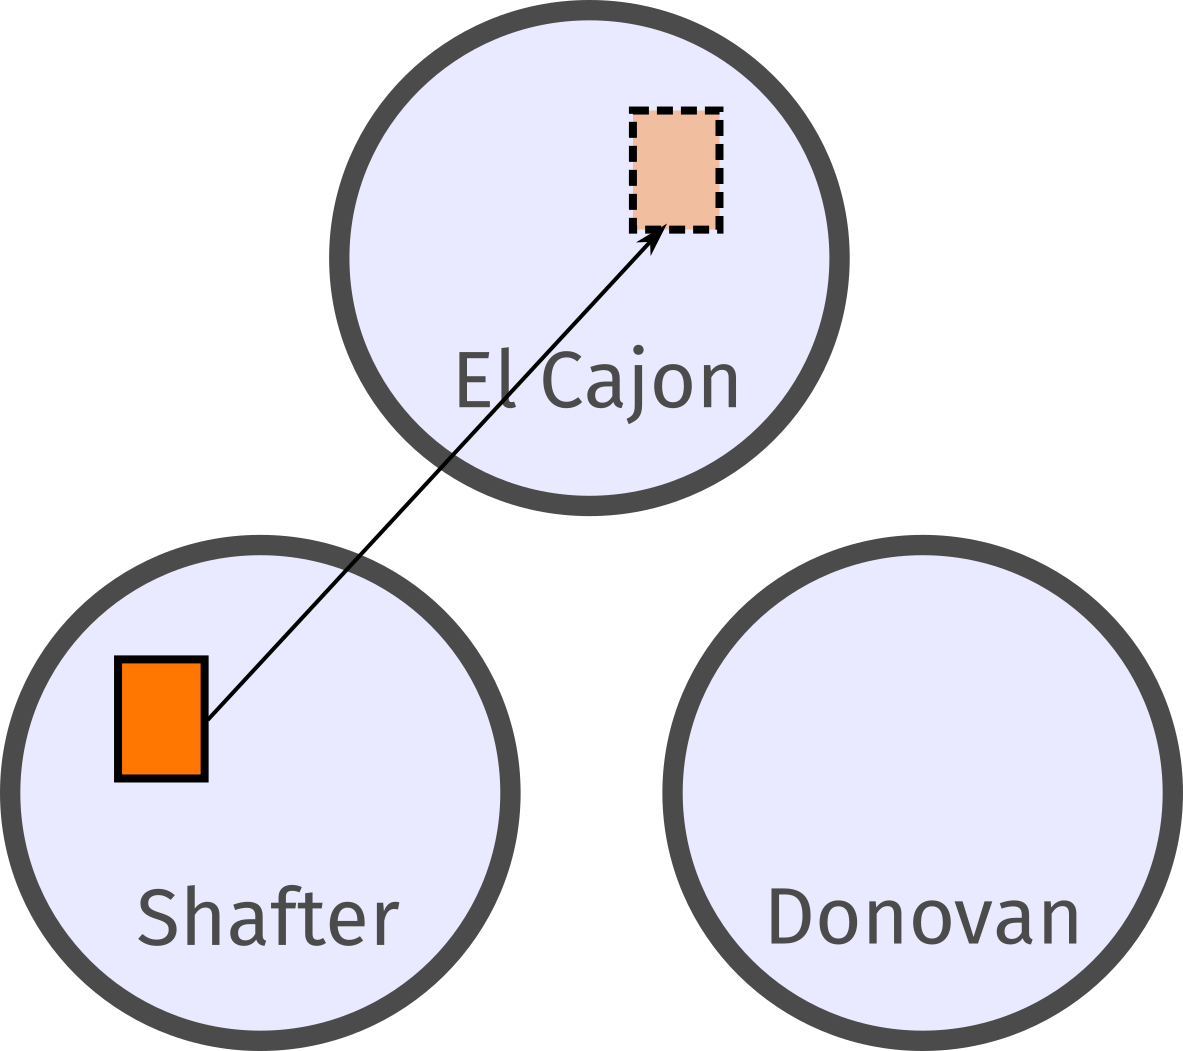
\includegraphics[width=\textwidth]{writeup/img/level1.png}
\caption{Level 1}
\end{subfigure}
~
\begin{subfigure}{0.23\textwidth}
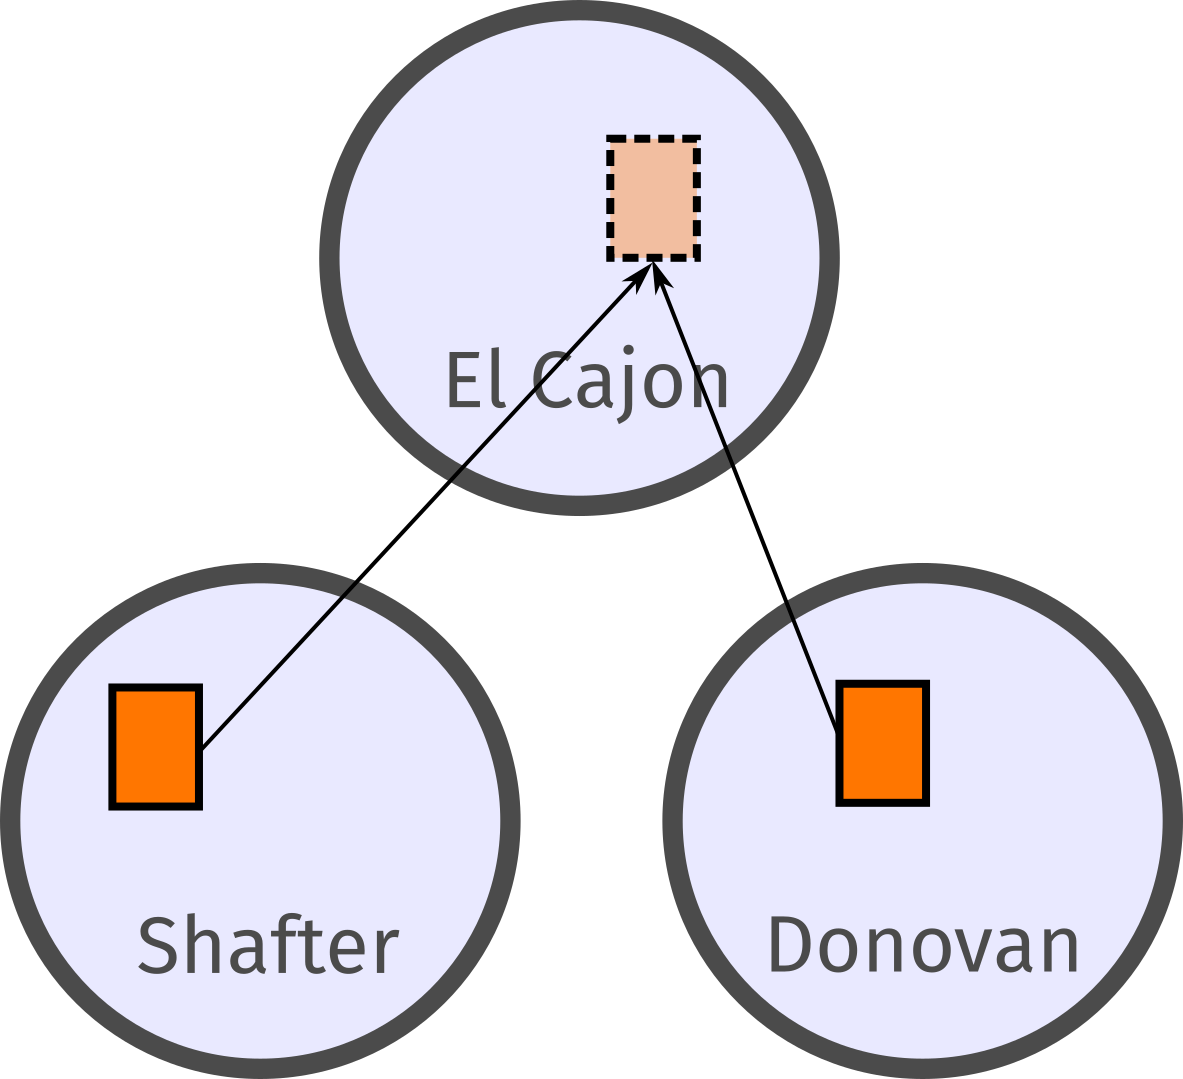
\includegraphics[width=\textwidth]{writeup/img/level2.png}
\caption{Level 2}
\end{subfigure}
~
\begin{subfigure}{0.23\textwidth}
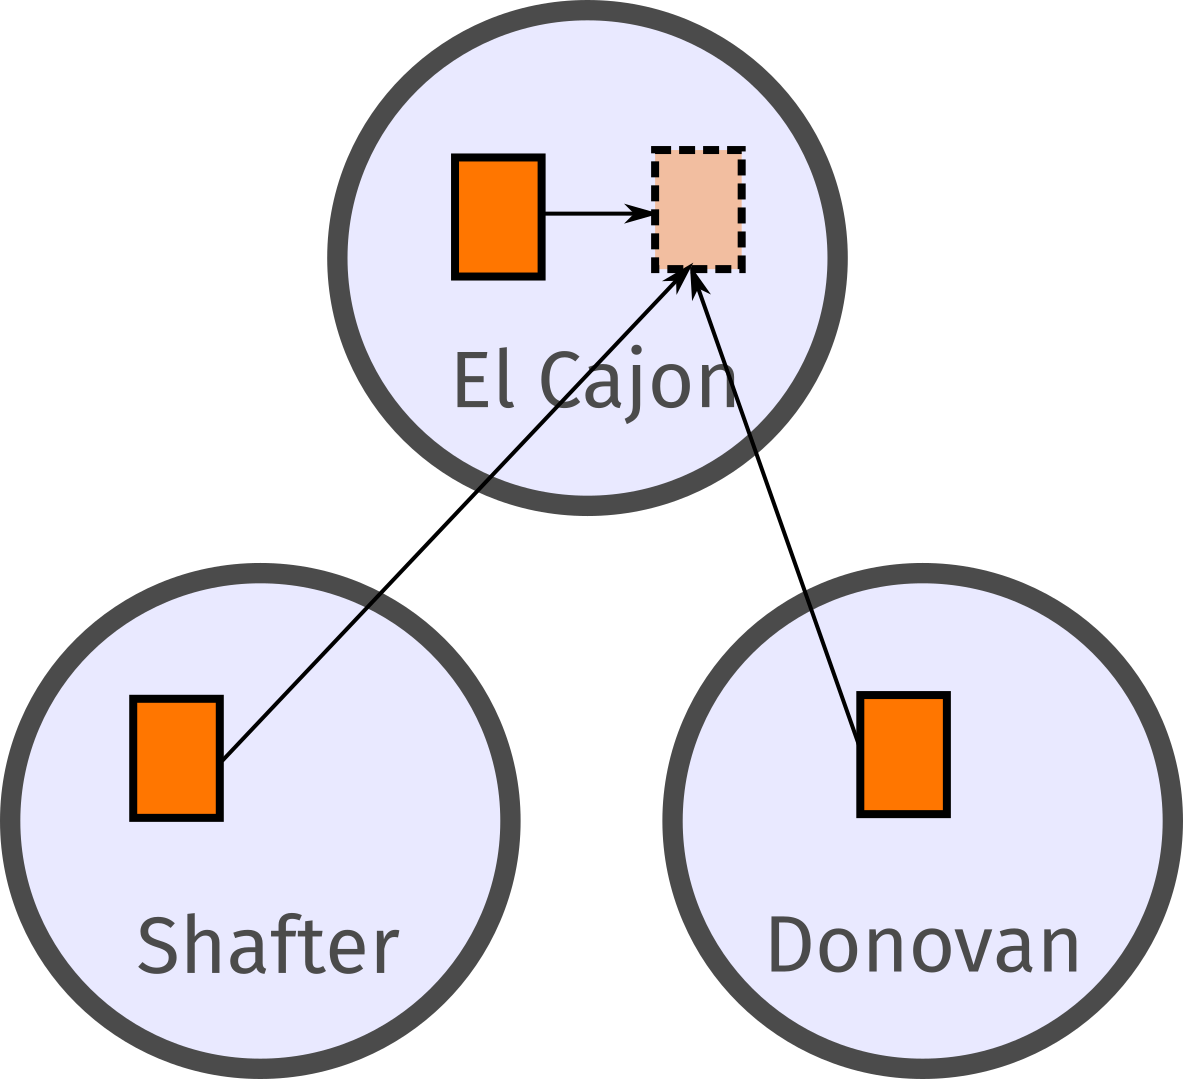
\includegraphics[width=\textwidth]{writeup/img/level3.png}
\caption{Level 3}
\end{subfigure}
\caption{Graphical depiction of training versus testing for the Level 0 through Level 3 benchmarks.  The Level 0 and 3 benchmarks test on a training site using held out data.  The Level 1 and 2 benchmarks train and test on different sites, also using held out data for consistency.}
\end{figure}

In the Level 0 and Level 3 benchmarks, the training and testing data distributions have explicit overlap, whereas in Level 1 and 2, there is no explicit overlap. We expect performance on Level 0 to be the best, as the training and testing distributions are identical.  We expect performance on Level 3 to be similar, due to the overlap in training and testing distributions. We expect performance on Level 1 to be the worst, as the training distribution is the narrowest and with no explicit overlap, whereas we expect performance on Level 2 to be between Level 1 and Level 3, for although there is no explicit overlap, the overall training distribution will be wider, forcing the models to be more general and possibly affording more implicit overlap.  Furthermore, we expect higher capacity models to overfit more to the training data set, and as a result, have the largest gap between Level 0 and Level 1. Thus, we expect linear regression to have more consistent performance across the benchmarks, albeit at relatively high error, followed by the 2-layer neural network, 4-layer neural network, and finally the random forest.

We ran each benchmark across all possible permutations of location and sensor package, measuring six metrics: root mean squared error (rMSE), centered root mean squared error (crMSE), mean absolute error (MAE), the coefficient of variation of mean absolute error (CvMAE), mean bias error (MBE), and coefficient of determination ($R^2$). The results for MAE of the baseline models are plotted in Figure~\ref{fig:results-linear}.  Details can be explored further in Table~\ref{fig:six-errors-table} in Appendix~\ref{app:six-errors}.

\begin{figure}[t]
\centering
\begin{subfigure}{0.45\textwidth}
\includegraphics[width=\textwidth]{\baselinedir/NO2" "MAE_test.png}
\caption{NO\textus{2}}
\end{subfigure}
\begin{subfigure}{0.45\textwidth}
\includegraphics[width=\textwidth]{\baselinedir/O3" "MAE_test.png}
\caption{O\textus{3}}
\end{subfigure}
\caption{Mean absolute error (MAE) boxplots for NO\textus{2} and O\textus{3}, for the Level 0 through Level 3 benchmarks.}
\label{fig:results-linear}
\end{figure}

We observe that on average, as model capacity increases, Level 0 error decreases. This is consistent across both NO\textus{2} and O\textus{3} prediction and reflects the ability of the model to fit the training distribution. Concerning model transferability, we find that consistently, \emph{all models suffer significant error when tested on different locations}. Level 1 and 2 benchmarks reflect the ability of a model to generalize to a distribution it hasn't seen before and we see that in these benchmarks, errors are much higher and the gaps between models are much smaller. Furthermore, Level 2 error is slightly lower on average than Level 1 error. By adding data from another site, effectively widening the training distribution, the models are slightly more robust to the unseen testing distribution. Level 3 performance aligns closely with Level 0 performance, which is to be expected, since in both cases the training distribution contains the testing distribution.

Across baselines, we observe that on average, linear regression has the highest error on all the benchmarks. However, its errors across the Level benchmarks are more consistent than the other models, suggesting that low-capacity linear regression is more robust to transfer. On the other hand, random forests have on average the lowest error, but have the most inconsistent results across the Levels. The results indicate a tradeoff between model capacity and robustness to transfer, consistent with our intuitions about model overfitting and generalization. Neural networks lie in between linear regression and random forests, and offer a tradeoff between low error and consistent error. 

\iffalse

\begin{itemize}
    \item  \emph{Current techniques assume that the conditions of sensor use match those of calibration.  How reasonable are these assumptions in practice?}
    \begin{itemize}
        \item Summarize the results of training on one location and testing on the others, compare the results across MLR, NN, and RF 
        \item Discuss the implications of these results, what does it mean for groups that are calibrating sensors in one location in a city and then moving them to new locations? Or groups calibrating in one city and deploying in another city? Is the drop in performance worse for moving sensors to a new city versus a new location in the same city (this could be valuable information for other researchers and regulatory agencies) Also, out of the quantification techniques tested (MLR, NN, RF) which would be recommended for different situations?
    \end{itemize}
    \item When they fail, what are the underlying causes of those failures?  (E.g., variance in humidity, temperature, barometric pressure, or background pollutants.)
    \begin{itemize}
        \item When we have a drop in performance is there still any valuable information in the data (i.e., are the trends still there, is it simply a shift causing the poorer performance?) -> a time series of training data from one San Diego site and that same model tested at the other San Diego site and the Shafter site could help us figure this out. (plot model tested on other site)
        \item Can these drops in performance be attributed to mainly a change in environmental and pollutant distributions between sites OR do different overall/background compositions at sites (based on environmental differences, different sources near and far, etc.) play a large role.
        \item different data distribution
        \item overfitting to environment experiments
        \item include data about RF leaves
    \end{itemize}
\end{itemize}
\fi


\begin{figure}[t]
\centering
\begin{subfigure}{0.33\textwidth}
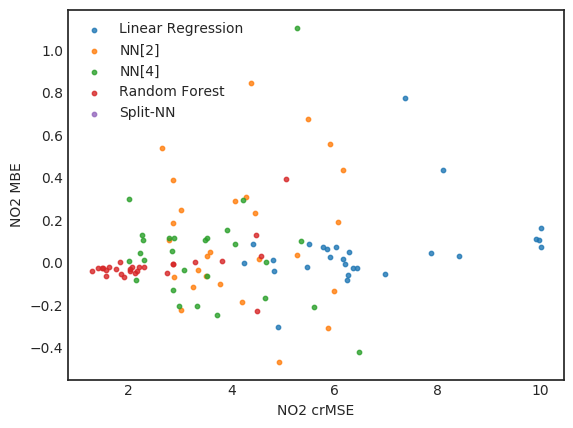
\includegraphics[width=\textwidth]{\baselinedir/NO2_level0_test_target.png}
\caption{Level 0 (NO\textus{2})}
\end{subfigure}
\begin{subfigure}{0.33\textwidth}
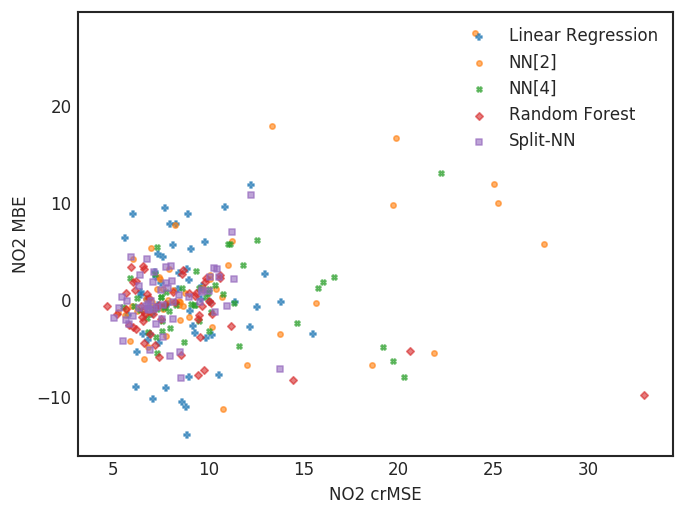
\includegraphics[width=\textwidth]{\baselinedir/NO2_level1_test_target.png}
\caption{Level 1 (NO\textus{2})}
\end{subfigure}
\begin{subfigure}{0.33\textwidth}
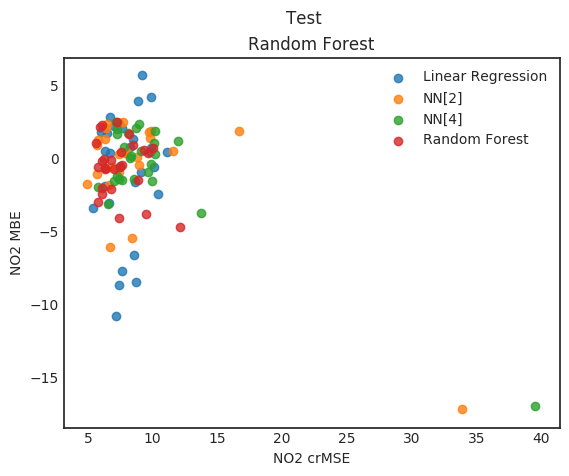
\includegraphics[width=\textwidth]{\baselinedir/NO2_level2_test_target.png}
\caption{Level 2 (NO\textus{2})}
\end{subfigure}
\begin{subfigure}{0.33\textwidth}
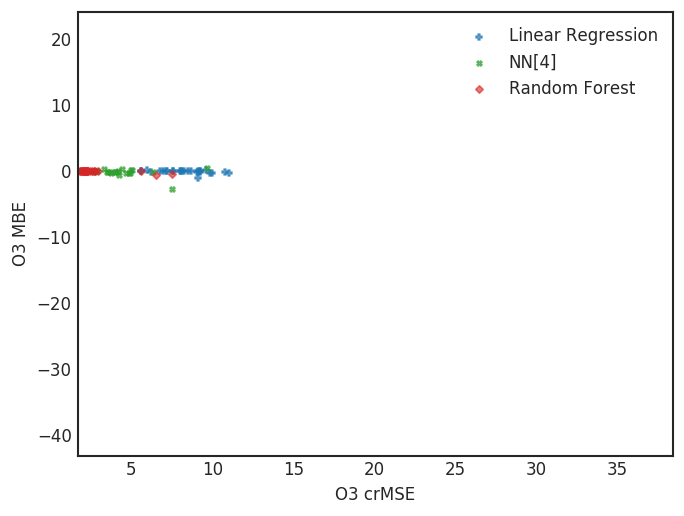
\includegraphics[width=\textwidth]{\baselinedir/O3_level0_test_target.png}
\caption{Level 0 (O\textus{3})}
\end{subfigure}
\begin{subfigure}{0.33\textwidth}
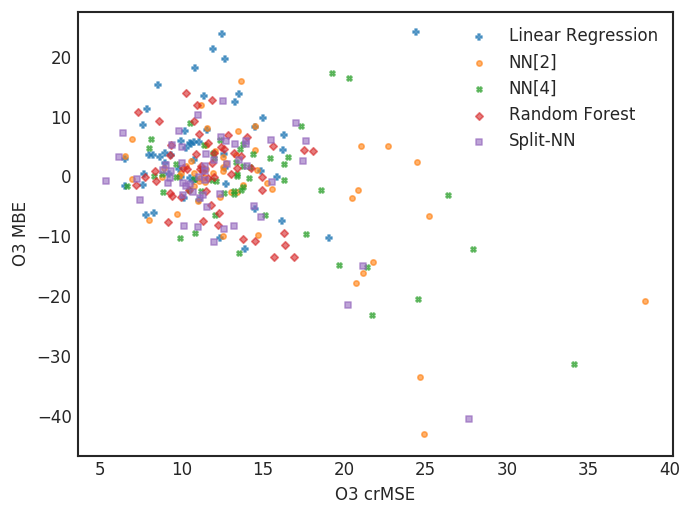
\includegraphics[width=\textwidth]{\baselinedir/O3_level1_test_target.png}
\caption{Level 1 (O\textus{3})}
\end{subfigure}
\begin{subfigure}{0.33\textwidth}
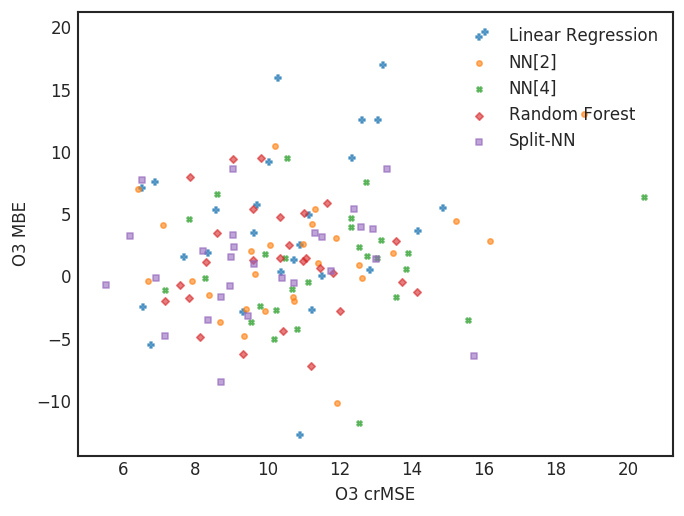
\includegraphics[width=\textwidth]{\baselinedir/O3_level2_test_target.png}
\caption{Level 2 (O\textus{3})}
\end{subfigure}
\caption{Target plots for Level 0 through Level 2 for both NO\textus{2} and O\textus{3}.}
\label{fig:target-plots-levels}
\end{figure}

To better understand how model performance degrades, we produced target plots, which visualize the tradeoff between centered error and bias  error (Figure~\ref{fig:target-plots-levels}).  The target plots indicate that while error approximately doubles when there is no explicit overlap in the distribution, model bias is many times larger. The increase in bias is more pronounced in the higher capacity models. Furthermore, despite the higher capacity models showing better error and bias in a Level 0 benchmark, the models have very similar error-bias tradeoffs in a Level 1 benchmark, indicating that even a high-capacity model cannot avoid this performance degradation.  Finally, in comparing the Level 1 and Level 2 plots, we observe that adding an additional (no-overlapping) site primarily reduces bias.  The Level 3 plots were very similar to the Level 0 plots and were excluded from Figure~\ref{fig:target-plots-levels} for brevity.

In general, however, we observe that model performance degrades non-trivially
when moved to different locations. This decrease in performance could result in overconfidence in a sensor's readings, potentially affecting downstream decisions. We briefly analyze the properties of our data that could result in overfitting by first investigating how data distributions across sites and times differ. Over each location and round, pollutant values can be highly variable. This is reflected, for example, in \autoref{fig:no2-rounds} where Shafter has higher values of NO\textus{2} in Round 1 and 2 but lower in Round 3. Furthermore, in \autoref{fig:o3-rounds}, the distribution of O\textus{3} changes remarkably across round and location. Similarly, temperature and humidity change significantly across location and round, which can be seen in \autoref{fig:temperature-rounds} and \autoref{fig:humidity-rounds}.

%\todo{(in the above, perhaps add something like: the model is overfitting to ambient environmental conditions and not the sensor reading. Many pollutants change with the diurnal cycle of the earth (eg. NO\textus{2} turning into O\textus{3} only when there is UV light, so NO\textus{2} is bigger at night, which is typically cooler and more/less humidity).)}.

A question that remains is to what degree overfitting or unique (non-overlapping) distributions of environmental data at the sites is contributing to the failure of the high capacity models to transfer well.  In an effort to better understand what may be driving the drop in performance of the high capacity models when boards are moved, we examined error density plots for temperature and humidity for the Level 1 benchmarks. In these types of plots, one of the predictors, such as temperature or humidity, is plotted against the error for all three sites in a single plot.  Figure~\ref{fig:error-density} displays the error density plots for absolute humidity against the error for the O\textus{3} estimation, for both the linear regression and random forest models (See the remaining plots in Appendix~\ref{sec:remaining-error-density-plots}). These plots illustrate how the magnitude of error varies with respect to higher or lower predictor values as well as how different pairs of training and testing sites compare. There are a couple of things we can derive from this collection of plots.  First, we observe that the pollutant concentrations at the Shafter site are difficult to predict, except for random forest when trained at Shafter itself (Figure~\ref{fig:error-density}f). The Shafter site was spatially far from the other sites and likely had a unique composition of background pollutants and ambient environmental conditions.  Second, we observe that when training a random forest model at one site and testing it at a different site (Figure \ref{fig:error-density}, bottom row), the error density plots look similar to the results from the linear regression models (Figure \ref{fig:error-density}, top row) despite the higher capacity of random forest models.  We observe that the greater errors at the Shafter site are occurring at humidity values that were seen in the training data set (more centrally in the plot), as is evident by their representation in the Donovan data. This implies that these errors did not occur at humidity values that have been extrapolated beyond the original training data set, but rather from overfitting at values in the distribution.  This leads us to conclude that overfitting is the reason random forest's net performance in transfer is not much better than linear regression.

%For example, in Figures~\ref{fig:error-density}a-c show all combinations of train and test for linear regression.  We note the overall similarity of these three combinations.  The one anomaly that we observe is that the model trained at the Donovan site performs particularly poorly at the Shafter site.  

%training occurs at the Donovan site and the error density pattern seen at the testing site in nearby El Cajon, is fairly comparable.  However, at the second testing site, Shafter, the error is greater. Furthermore, the greater error at the Shafter site is occurring at humidity values that were seen in the training data set (more centrally in the plot), as is evident by their representation in the Donovan data. In other words, these are not humidity values that have been extrapolated beyond the original training data set. The same pattern holds true for temperature (See Appendix~\ref{fig:remaining-error-density-plots} for details): there are greater errors occurring at Shafter as opposed to El Cajon and at least a portion of these errors are not occurring at temperature values that were unseen during training. Thus, if the poorer performance by the linear model in Shafter is not attributable to environmental conditions that the model was simply not trained for, then there must be another factor driving this poor performance. Given the differences in source types around the El Cajon versus the Shafter site, we expect the Shafter site to be more different from Donovan than El Cajon, and one potential driver of the poor model performance is the differing levels and compositions of background pollutants.  Given the consistency of this behavior across the plots, it supports the hypothesis that the background composition of pollutants impact low-cost sensors and play a role in model performance (in addition to the well-established impacts from environmental conditions).  Figure~\ref{fig:error-density}b supports these conclusions as again we see fairly comparable error between the two San Diego sites and higher error at the Shafter site at humidity values represented in the training data set.  However, in this plot we can also see that the error at the Donovan site is higher at high and low humidity and temperature values not represented in the original training data set, or where extrapolation is occurring.  This is a limitation we would expect, mainly that pollutant estimations are less trustworthy when the model is required to extrapolate beyond the original training values. Finally, Figure~\ref{fig:error-density}c illustrates how training at the Shafter site results in enhanced and comparable error at both San Diego sites, again supporting the previous observations given that we would expect the two San Diego sites to be more similar to each other and substantially different from the Shafter site.

%When we examine these same plots for the random forest model in the bottom half of Figure~\ref{fig:error-density}, we see a similar pattern, but the relative difference in error between the training and testing sites is amplified, even between the two San Diego sites.  The similar pattern corroborates the evidence that differences in background pollutants between Shafter and the San Diego sites are a contributing factor. \todo{I think it might be a little more accurate to say that the random forest model is overfitting to all of the conditions of the training site, both environmental and background, b/c the patterns seem pretty different from the linear models and we don't see the same differences between different training/testing pairs.  WGG: I think we do; note that the sites in DEF are out of order wrt to ABC, making it confusing.}   A closer look at Figure~\ref{fig:error-density}e reveals more, however.  As noted with Figure~\ref{fig:error-density}b, the El Cajon site has a narrower distribution of humidity than the Donovan site, resulting in higher errors due to failures in extrapolation.  In Figure~\ref{fig:error-density}e, we see this effect is strongly amplified with the random forest model, providing further evidence that the high capacity of the random forest model is strongly overfitting to the training site, limiting the ability of the models to extrapolate, and hence transfer.  We are are led to conclude that the relatively amplified errors across all three plots is due to overfitting.  As a consequence, random forest's net performance in transfer is not much better than linear regression, especially when the environmental conditions are similar.

\todo{WGG: above, cite Joanna's paper if we corroborate.}

%\begin{figure}[H]
%\centering
%\begin{subfigure}{0.45\textwidth}
%\includegraphics[width=\textwidth]{\baselinedir/subu/error_density_temperature_donovan_NO\textus{2}.png}
%\caption{Temperature - Linear Regression (NO\textus{2}, Donovan)}
%\end{subfigure}
%\begin{subfigure}{0.45\textwidth}
%\includegraphics[width=\textwidth]{\baselinedir/subu/error_density_temperature_donovan_O\textus{3}.png}
%\caption{Temperature - Linear Regression (O\textus{3}, Donovan)}
%\end{subfigure}
%\caption{}
%\label{fig:error-density}
%\end{figure}

\begin{figure}[t]
\centering
\begin{subfigure}{0.33\textwidth}
\includegraphics[width=\textwidth]{\baselinedir/linear/error_density_absolute-humidity_donovan_O3.png}
\caption{LR, trained at Donovan}
\end{subfigure}
\begin{subfigure}{0.33\textwidth}
\includegraphics[width=\textwidth]{\baselinedir/linear/error_density_absolute-humidity_elcajon_O3.png}
\caption{LR, trained at El Cajon}
\end{subfigure}
\begin{subfigure}{0.33\textwidth}
\includegraphics[width=\textwidth]{\baselinedir/linear/error_density_absolute-humidity_shafter_O3.png}
\caption{LR, trained at Shafter}
\end{subfigure}
\begin{subfigure}{0.33\textwidth}
\includegraphics[width=\textwidth]{\baselinedir/subu/error_density_absolute-humidity_donovan_O3.png}
\caption{RF, trained at Donovan}
\end{subfigure}
\begin{subfigure}{0.33\textwidth}
\includegraphics[width=\textwidth]{\baselinedir/subu/error_density_absolute-humidity_elcajon_O3.png}
\caption{RF, trained at El Cajon}
\end{subfigure}
\begin{subfigure}{0.33\textwidth}
\includegraphics[width=\textwidth]{\baselinedir/subu/error_density_absolute-humidity_shafter_O3.png}
\caption{RF, trained at Shafter}
\end{subfigure}
\caption{Error density plots for O\textus{3} versus absolute humidity for both Linear Regression (LR) and Random Forest (RF) in a Level 1 benchmark.}
\label{fig:error-density}
\end{figure}


\subsection{Benefits of Sharing Data Across Sensor Packages}
In this section, we evaluate the split-NN model architecture's utility for improving the transferability of a calibration model.  The novelty of the split-NN model for calibrating a board's model is its ability include (normalized) data from other boards.  Given that the resources for calibration are limited, the research questions for split-NN revolve around how boards could be best distributed to available field sites.  For a standard modeling technique like random forest, a board has to be placed at three sites for three rounds to experience the wide training distribution that achieves the exceptional transferability observed in the Level 3 benchmarks.  However, with the split-NN model, multiple boards can be deployed for just one round, divided equally across the sites.  Then the data from their boards can be normalized and shared to produce models that we hypothesize to be of similar quality to a Level 3 benchmark, but in one-third the time, in a single round.

To help reveal the value of calibrating multiple boards at once, we performed three one-round benchmarks: 1 board at each of the three sites, 2 boards at each of the three sites, and 3 boards at each of the three sites.  In each of these conditions, a board is trained from a single round of data and tested on the other locations, not its own.  In this vein, these are all Level 1 benchmarks, thus we compare the resulting models against our Level 1 baselines. We expect the split-NN to outperform Level 1 random forest, as the inclusion of more data helps reduce bias. In the situation that there are more boards to calibrate than there are training sites, there is an opportunity to also incorporate data additional boards at the same site.  We expect that a greater multiplicity of boards at each site will produce slightly better models, but with diminishing returns. We evaluated this effect by including training split-NN's with increasing numbers of boards at each site, indicated by the variants Split-NN (3), Split-NN (6), and Split-NN (9), corresponding to having one board at each site, two boards at each site, and three boards at each site.  We perform a similar assessment with two-round (Level 2) benchmarks, still testing only on sites that a board hasn't been trained on.  As previously, we control for the total amount of data, simulating an abbreviated deployment for the Level 2 benchmarks.

Figure~\ref{fig:split-results-lrfe}a-b shows that the split-NN model on average has slightly lower MAE in the Level 1 benchmarks when compared to the random forest model. We see in and Figure~\ref{fig:split-results-lrfe}c-d that the gap widens with the Level 2 benchmark, indicating that the Split-NN model is able to better capitalize on the additional data. The results also support our hypothesis that we receive diminishing returns with additional data. 

The marginal improvement seen in the Level 1 benchmarks has two possible causes.  One is that there is insufficient overlapping of the pollutant distributions across the sites, compromising the first-stage linear regression to correct bias.  The other is that the difference in behavior among sensors is non-linear.   The fact that using two rounds of data (Level 2) does better does much better suggests that lack of overlap in data distributions plays a role.  To gain further insight on this, we replaced the first stage linear regression with a full neural net.  .... Figure~\ref{fig:split-results-nnfe}

%We also find that training the split models on more locations as opposed to a wider range of time achieves marginally lower error, though both exhibit similar performance overall.

\begin{figure}[H]
\centering
\begin{subfigure}{0.45\textwidth}
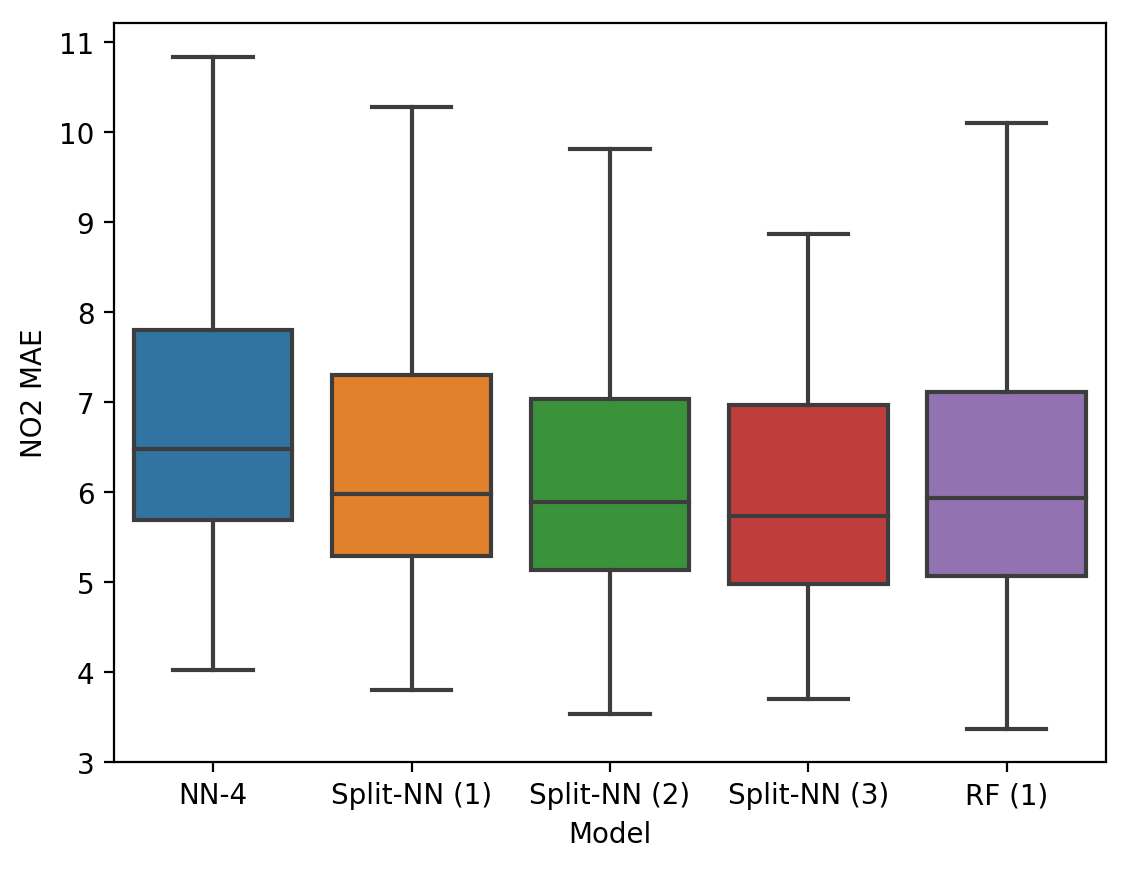
\includegraphics[width=\textwidth]{results/split-no2-location-mae}
\caption{Level 1 NO\textus{2}}
\end{subfigure}
\begin{subfigure}{0.45\textwidth}
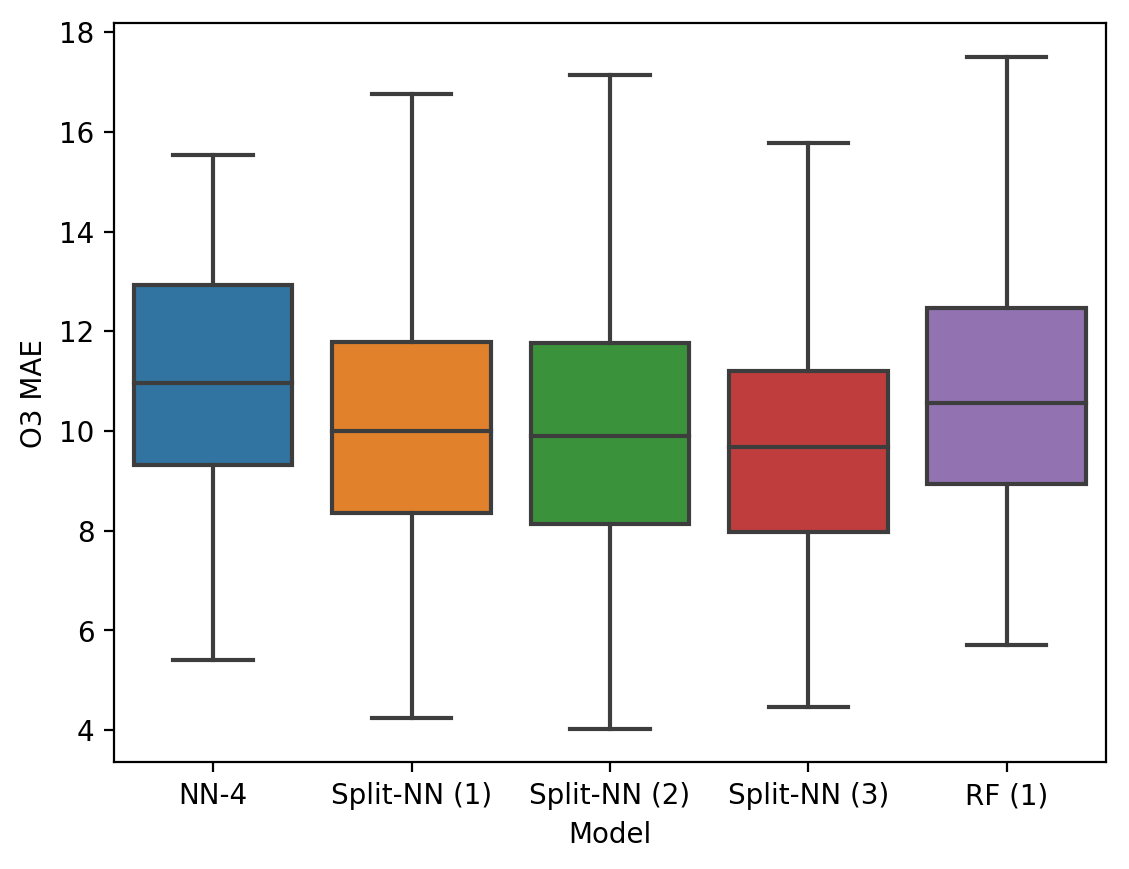
\includegraphics[width=\textwidth]{results/split-o3-location-mae}
\caption{Level 1 O\textus{3}}
\end{subfigure}
\begin{subfigure}{0.45\textwidth}
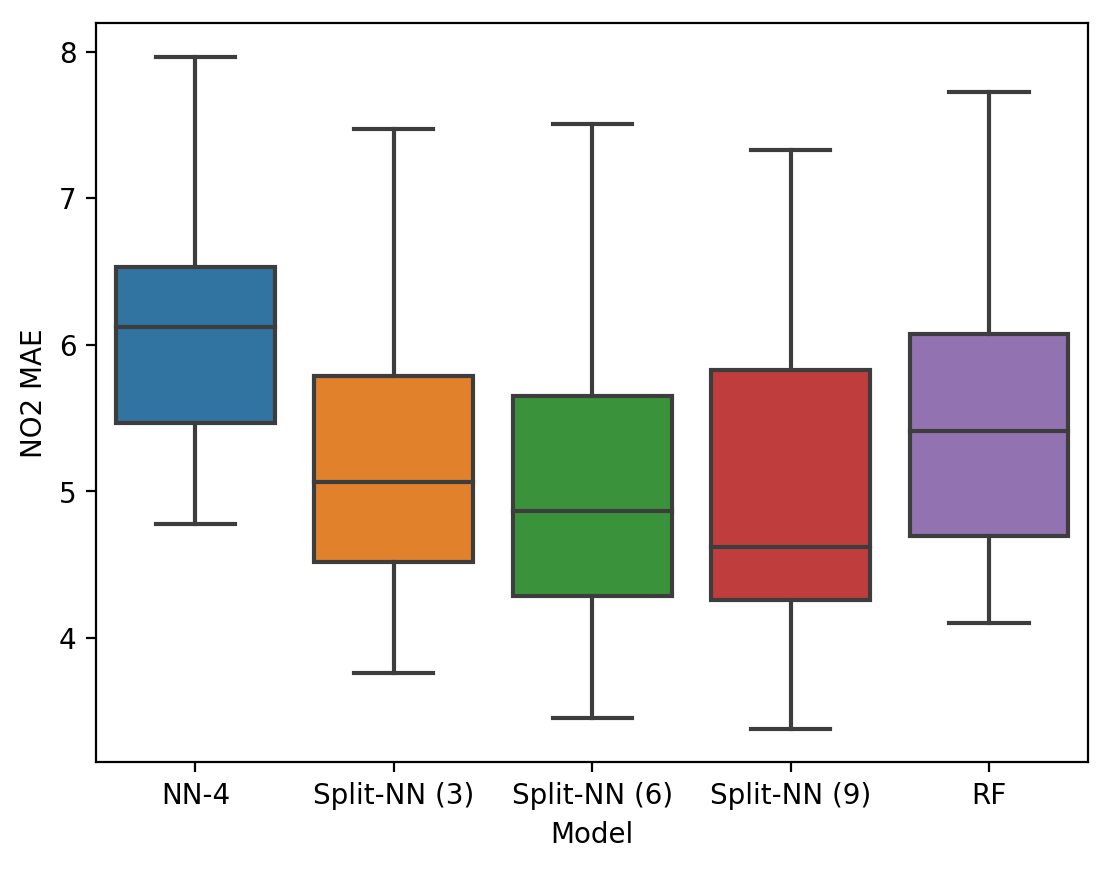
\includegraphics[width=\textwidth]{results/split-no2-location-level2-mae}
\caption{Level 2 NO\textus{2}}
\end{subfigure}
\begin{subfigure}{0.45\textwidth}
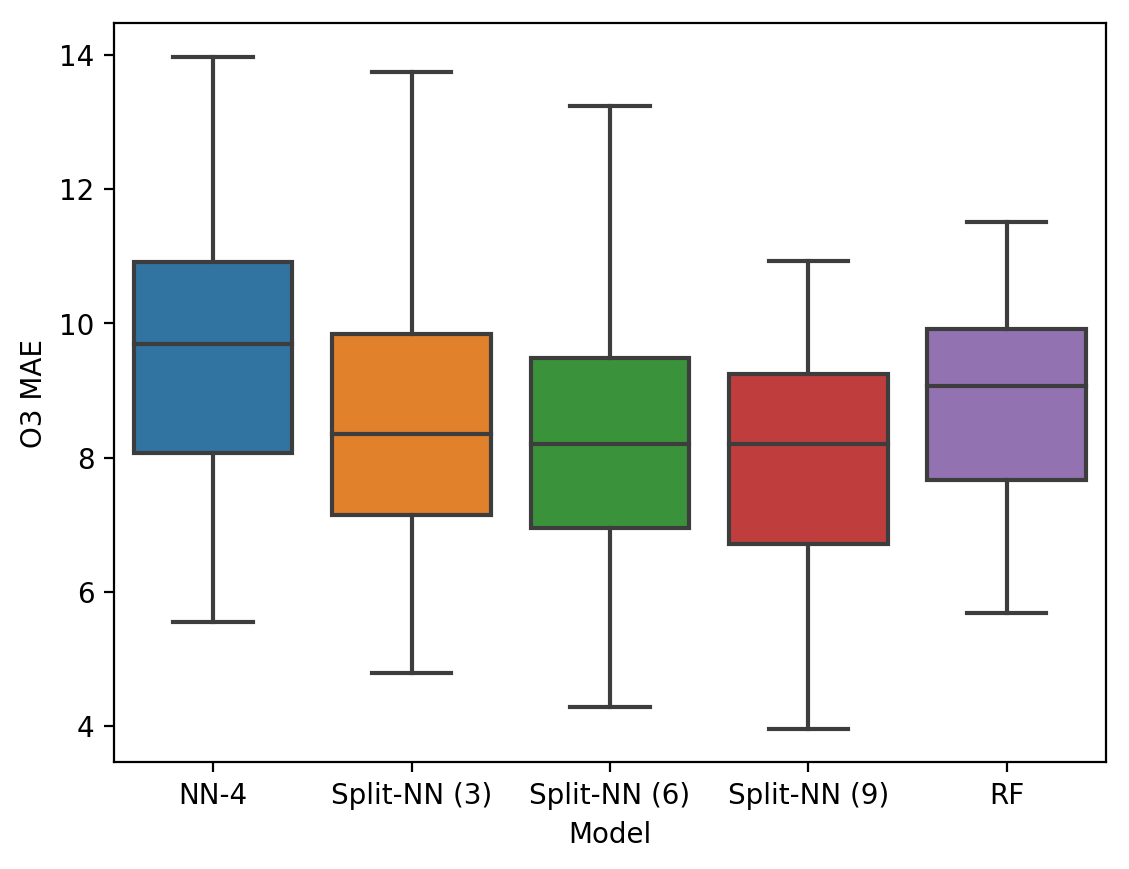
\includegraphics[width=\textwidth]{results/split-o3-location-level2-mae}
\caption{Level 2 O\textus{3}}
\end{subfigure}
\caption{Results of evaluating the split-NN model with a linear regression first stage, compared against the RF model in both Level 1 and Level 2 comparisons. The split-NN model has a lower mean and median error in all conditions. Boxplots are pictured without outliers for clarity.}
\label{fig:split-results-lrfe}
\end{figure}

% Seasonal plots
%\begin{subfigure}{0.45\textwidth}
%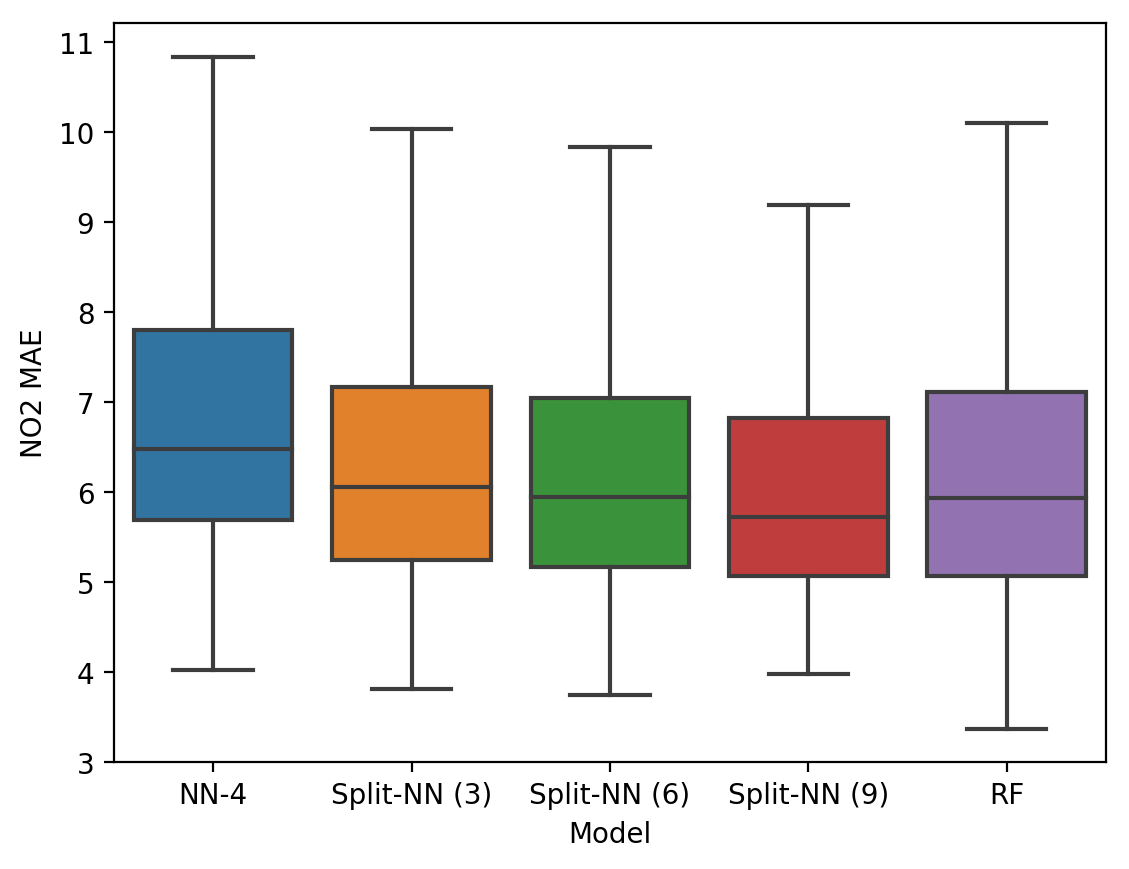
\includegraphics[width=\textwidth]{results/split-no2-seasonal-mae}
%\caption{Level 1 Seasonal Split-NN neural network results (NO\textus{2})}
%\end{subfigure}
%\begin{subfigure}{0.45\textwidth}
%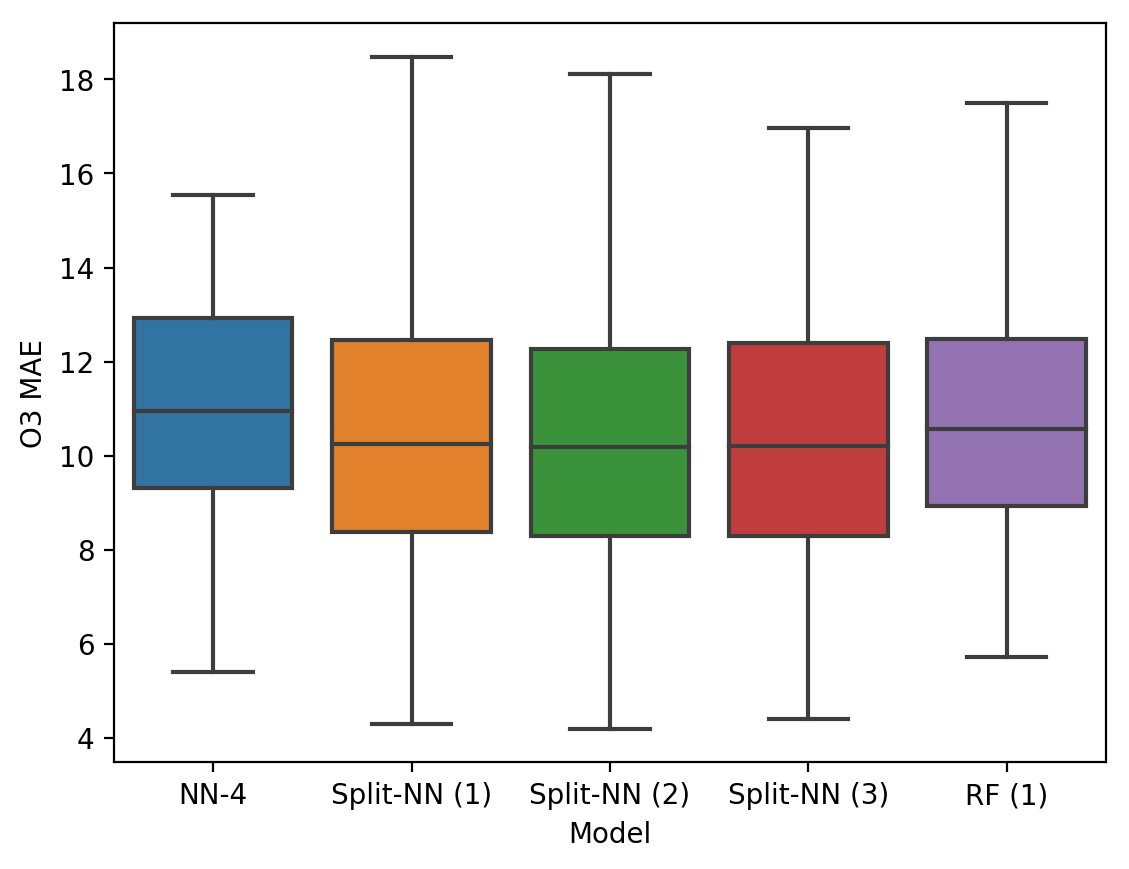
\includegraphics[width=\textwidth]{results/split-o3-seasonal-mae}
%\caption{Level 1 Seasonal Split-NN neural network results (O\textus{3})}
%\end{subfigure}
%\begin{subfigure}{0.45\textwidth}
%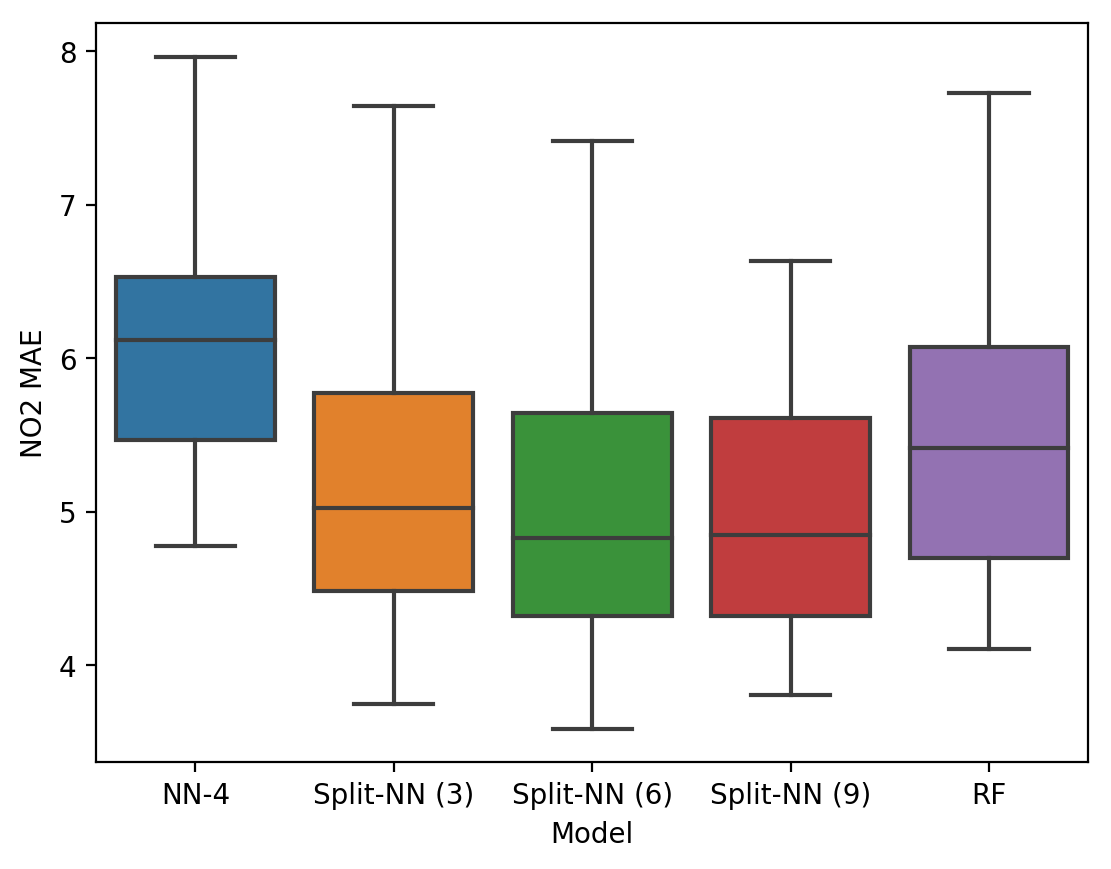
\includegraphics[width=\textwidth]{results/split-no2-seasonal-level2-mae}
%\caption{Level 2 Seasonal Split-NN neural network results (NO\textus{2})}
%\end{subfigure}
%\begin{subfigure}{0.45\textwidth}
%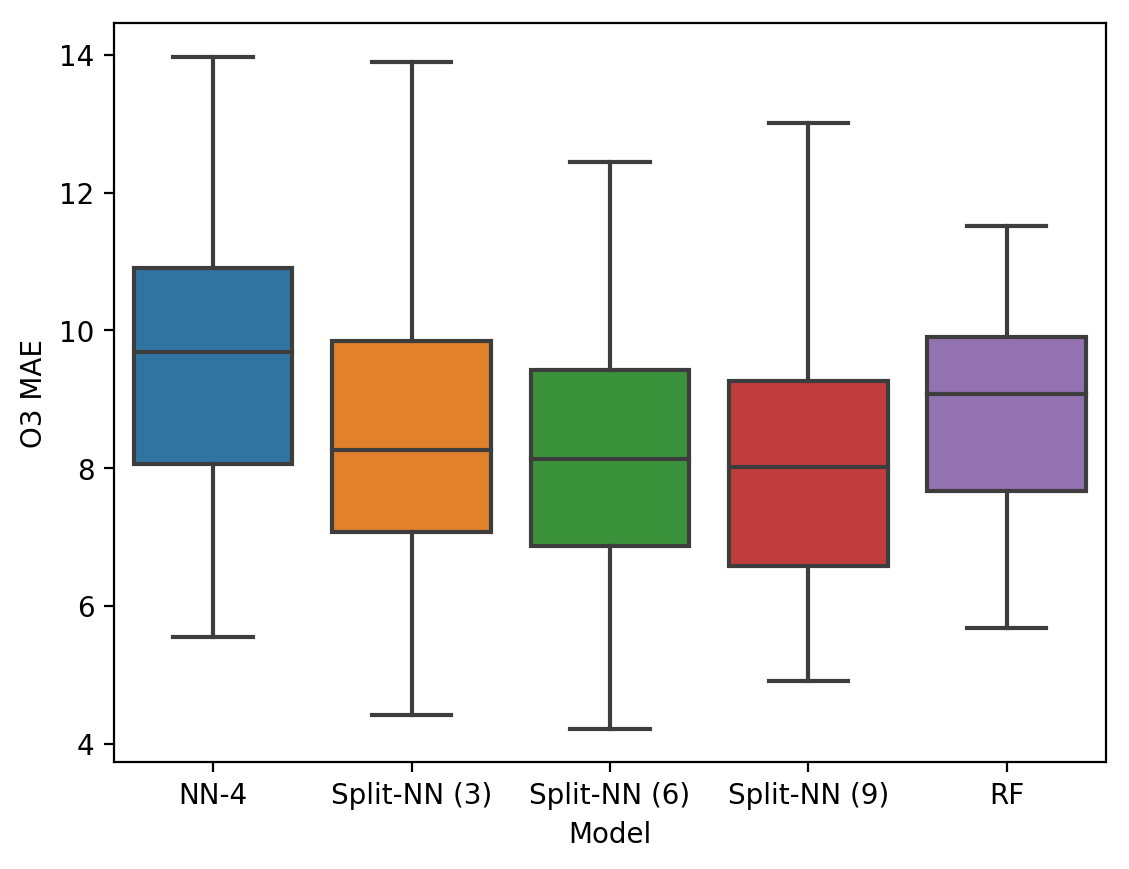
\includegraphics[width=\textwidth]{results/split-o3-seasonal-level2-mae}
%\caption{Level 2 Seasonal Location Split-NN neural network results (O\textus{3})}
%\end{subfigure}

\begin{figure}[H]
\centering
\begin{subfigure}{0.45\textwidth}
\includegraphics[width=\textwidth]{results/split-nnfe-no2-location-mae}
\caption{Level 1 NO\textus{2}}
\end{subfigure}
\begin{subfigure}{0.45\textwidth}
\includegraphics[width=\textwidth]{results/split-nnfe-o3-location-mae}
\caption{Level 1 O\textus{3}}
\end{subfigure}
\begin{subfigure}{0.45\textwidth}
\includegraphics[width=\textwidth]{results/split-nnfe-no2-location-level2-mae}
\caption{Level 2 NO\textus{2}}
\end{subfigure}
\begin{subfigure}{0.45\textwidth}
\includegraphics[width=\textwidth]{results/split-nnfe-o3-location-level2-mae}
\caption{Level 2 O\textus{3}}
\end{subfigure}
\caption{Results of evaluating the split-NN model with a neural net first stage, compared against the RF model in both Level 1 and Level 2 comparisons. The split-NN model has a lower mean and median error in all evaluations. Boxplots are pictured without outliers for clarity.}
\label{fig:split-results-nnfe}
\end{figure}

\iffalse
We also evaluated the calibration of a new sensor package using the split-NN approach. As described in Section~\ref{sec:split-nn}, rather than retraining a full calibration model when a new, uncalibrated sensor needs to be deployed, we can colocate it with an already-calibrated low-cost sensor. We then train a new sensor model for the new board, regressing to match the sensor model outputs from the colocated boards. Since the sensor model outputs intermediate values that are then fed into a global calibration model, we have effectively calibrated a new board just through the sensor model. Using this approach we find \todo{WGG: how?} that on average, \todo{WGG: is this additional error over doing it from scratch?  Sounds high.  Our new test will help here.} we incur 3.79 NO\textus{2} MAE and 6.07 O\textus{3} MAE.
\fi


%\begin{figure}
%    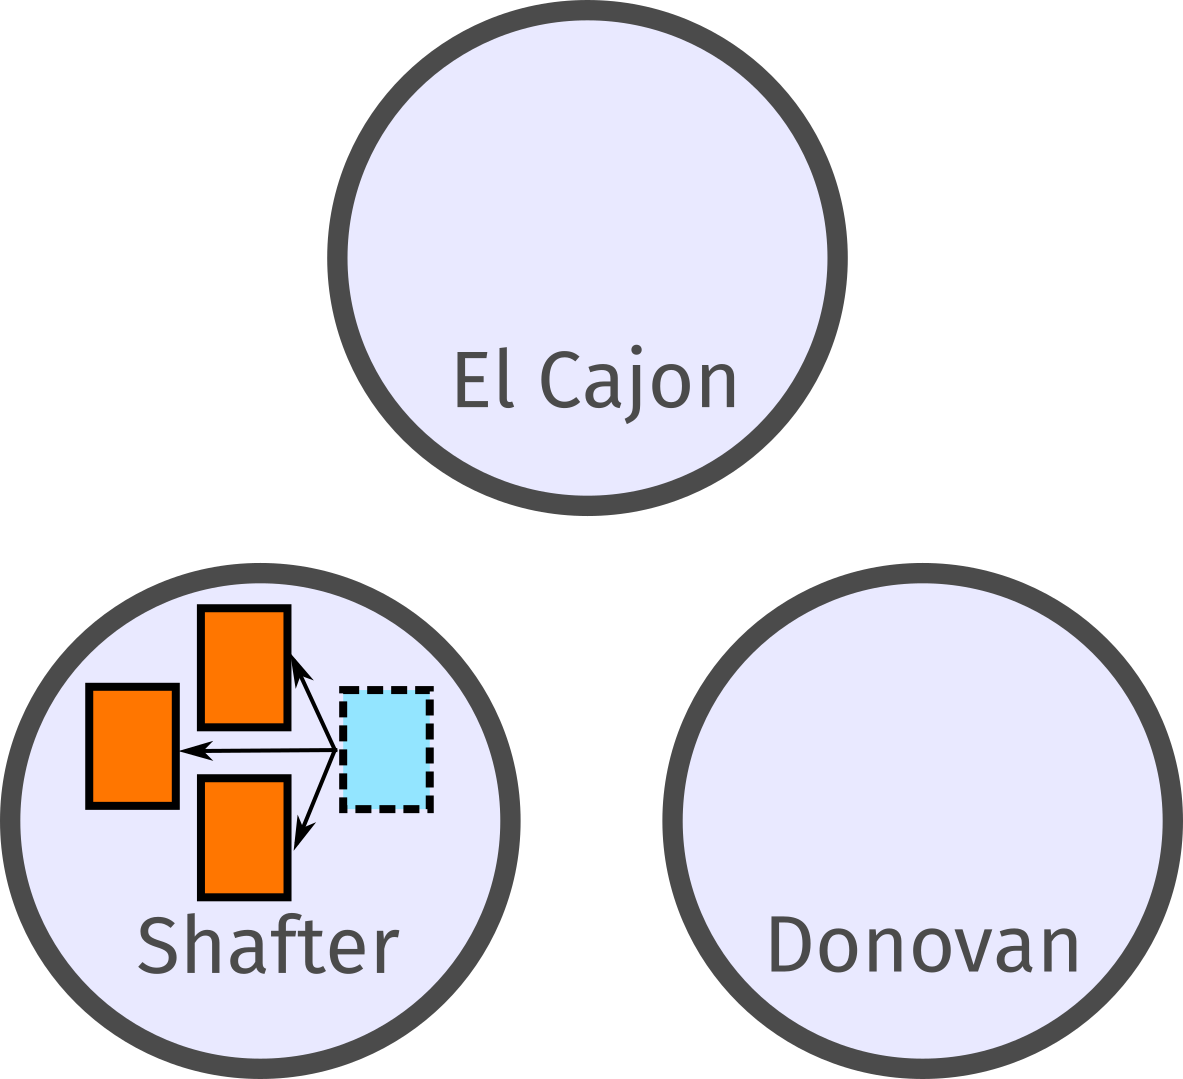
\includegraphics[width=0.3\textwidth]{writeup/img/levels-retrain}
%    \caption{Calibrating a new board $N + 1$}
%\end{figure}

\iffalse

\begin{itemize}
    \item Given these failure modes, how can data collection and model training be improved to overcome these failures?
      \begin{itemize}
          \item Collect data from multiple sites and either:
          \begin{itemize}
            \item Average models over multiple diverse locations 
            \item Pool all the data together and build a single model
          \end{itemize}
      \end{itemize}
    \item Given that it is typical to calibrate many sensors, how should calibration data from multiple sensors be employed to achieve the best results?
      \begin{itemize}
          \item Collect data from all sensors to be calibrated and build a single shared model
      \end{itemize}
    \item Finally, (how) can multiple-site techniques and multiple-sensor techniques be combined?
      \begin{itemize}
         \item Neural networks work, and random forest doesn’t, because they are more modular (differentiability)
      \end{itemize}
    \item Can a new sensor can be affordably and accurately calibrated without having to repeat the whole data collection cycle?
      \begin{itemize}
          \item Simple colocation with a single sensor
          \item Match new sensor to the global model through colocation with one of the calibrated sensors
      \end{itemize}
\end{itemize}
\fi

\subsection{Discussion}

As low-cost sensor studies move from understanding sensor signal performance to how this performance is affected by moving sensors to new sampling locations or utilizing them in new applications, it is important that the results are translated into best practices to support the collection of usable high quality data. This is particularly important given the interest in sensors by community-based organizations and citizen scientists. Although the present study examined only electrochemical O\textus{3} and NO\textus{2} sensors and the sampling sites were limited to three in California, it adds to a body of evidence that location matters in the calibration of low-cost sensors because the background environmental conditions matter.  With this in mind, we make the following observations and recommendations.

%Given that the present study examined only electrochemical O\textus{3} and NO\textus{2} sensors and the sampling sites were limited to three in California, there is a need to continue examining different sensors and to learn more about the consistency of results across locations and situations. 
We observed how prediction performance degrades when a sensor is moved to a new location, especially for high-capacity modeling techniques. In particular, training a complex random forest calibration model will likely result in very low error at a colocated site but can incur significant error at a different site. Although their predictions at a new site will have lower error than linear regression, the error they have at the training site will likely not be representative of their error in practice.  A linear model, on the other hand, despite not predicting as well at the training site, will not have significantly more error at testing time.  Thus, if it is important to know the likely error of your calibration model under transfer, it would be best to use a low-capacity method like linear regression.

When we drilled down to investigate the contributors to error when changing location, we found that bias error was a significant contributor in many cases. This is interesting because bias error indicates a loss of accuracy (a non-random additive error) rather than a loss of precision (random noise). This suggests that when moving a sensor to a new location, if the bias can somehow be detected, then it may be possible to make a bias correction to improve model performance. This result also motivates the use of the split neural network architecture, which has a model-specific correction stage that is designed to learn unbiased representations of sensor measurements.

We had expected that training at multiple sites would provide much better transferability, but the improvements were not substantial, suggesting that the high-capacity models were mostly improving due to implicit overlap in distributions and not actual generalization.  This suggests that calibration should be directed at capturing the widest conditions possible, for example using many field sites with varying conditions, so as to create an overlap between the distributions of training and use.  This recommendation is further supported by the observation that the Level 3 benchmarks performed nearly as well as the Level 0 benchmarks, in spite of carrying the load of a much wider distribution in the models.

The split-NN approach provides a potentially economical approach to creating overlap in distributions since sensors can share their data for calibration.  That is, when calibrating multiple sensors, rather than colocating multiple sensors at a field site and rotating those sensors over time, it makes sense to distribute the sensors to as many field sites as possible to capture the widest distribution of conditions.  More study will be required to see how well the split-NN approach scales.

\todo{WGG: graphs don't show this: Location Test will help.} Only when we employed the split-NN technique did we get the expected results.  
\todo{WGG: something about training a new sensor?}

%Considering these limitations, there are a number of recommendations drawn from the results of this study that may be useful for communities and citizens scientists interested in using low-cost sensors. 
% 
%\begin{itemize}
%    \item When conducting a “field calibration” (or colocating your sensors with trusted reference monitors), colocating your sensors at multiple reference locations will likely improve the reliability of the data from your sensors when they are moved to the field sites.
%    \item If you are conducting a field calibration and are unsure of how different your field sites are from your calibration site, consider choosing a simpler calibration model, such as a multiple linear regression model.
%    \item When conducting a field calibration, placing sensors at different colocation sites then pooling that data and building a calibration model built on data from multiple sites will result in a calibration model that is more robust in new locations. 
%end{itemize}

%Essentially, the recommendations presented here emphasize the need for thoughtful study design when using low-cost sensors. Users need to be thoughtful about where and how calibration is occurring, as well as any potential repercussions of a particular choice – for example the decision to use a high-capacity machine learning model.


%Previous text:
%
%\begin{itemize}
%    \item \todo{Model size}
%    \item \todo{Calibrate over a lot of sites}
%    \item If one doesn't have access to multiple sites (or only two instead of three), can multiple locations be approximated by just training longer at one site? \emph{maybe}
%    \item Translate what we've learned into practical advice for an average citizen scientist group - how can they use this information to improve their work and given typical real-world constraints where can they focus their efforts in order to get the best data quality possible (maybe this section should include a list of hypothetical) 
%\end{itemize}

\section{Conclusion}

As low-cost gas-phase sensors are increasingly being adopted for citizen science efforts and community-based studies, there is a need to better understand what contributes to accurate sensing.  A key question is how a change in background environmental or pollutant conditions, often unique to a location, affects accuracy.  A rotating deployment strategy enabled benchmarking the transferability of models and investigating how to improve accuracy. We found that overfitting is a concern, especially when transferring high-capacity models like random forest that are trained with data that will not be representative of the conditions of use. Our benchmarks indicate that widening the data distribution is a good strategy to make models more robust to transfer, but that the best results require the training distribution to contain the distribution encountered in use.  A tantalizing result is that much of the error introduced by transfer was bias, which may be correctable.  When multiple sensors based on the same technology are being trained at the same time, we found that a split neural network architecture increases the robustness of model transfer by giving a sensor's model access to normalized data from other sensors, even at other locations, hence widening the distribution without requiring additional data collection.  This method also enables accurately calibrating new sensors against existing calibrated sensors at incremental cost.

In the future work we will be extending this work to answer open questions that we believe are relevant to the future of low-cost sensor calibration.  As one example, there are questions about the effect of temporal resolution on accuracy. Currently, our MetaSense sensors are sampled every five seconds, but the ground-truth data provided from reference monitors is minute-averaged. By averaging our own sensor measurements every minute, we discard data that could be relevant for calibration. Recent advances in recurrent neural networks for sequence prediction might help leverage the high-resolution data for robust prediction. As a second example, a potential application of low-cost sensing is truly mobile sensing with person- or vehicle-mounted sensors. Deployments such as these will raise questions about the effects of mobility on sensing accuracy, such as rapidly changing conditions, with few studies to date~\citep{arfire2016mitigating}.

% A dynamic data distribution is a challenge that we hope our methods can generalize to.

\section{Acknowledgements}

We would like to thank partners at the San Diego Air Pollution Control District as well as San Joaquin Valley Air Pollution Control District for their support throughout this deployment. 

\iffalse
\begin{itemize}
    \item What is the tradeoff between resolution and accuracy, if any. 
    \item Mobility causes fast changes. Brief high exposures could be harmful.
    \item Our sensors change slowly, taking up to 30 seconds to respond to a change in signal
    \item Noise, Drift?
\end{itemize}
\fi

\bibliographystyle{copernicus}
\bibliography{main.bib}


%%%%%%%%%%%%%%%%%%%%%%%%%%%%%%%%%%%%%%%%%%%%%
%%%%%%%%%%%%%%%%%%%%%%%%%%%%%%%%%%%%%%%%%%%%%
\clearpage
\appendix
\setcounter{table}{0}

\iffalse
\section{Data}

We have been collecting data from nine boards
from three sites in southern California.
\begin{enumerate}
    \item El Cajon
    \item Donovan
    \item Shafter
\end{enumerate}
We have split up the boards and rotated the boards
between locations every two weeks (see \autoref{tab:board-rotations}).

We do not have CO data for Shafter and Donovan, so we will focus only on
O\textus{3} and NO\textus{2}.
\fi


\section{Environment and Pollutant Distributions}\label{Distributions}

%\todo{Have these been updated to reflect the data we are using? (i.e., from R2, R2, and R4}
%\todo{Recommend for the Distribution section just keep plots B5, B6, B8, B10 - those would be sufficient, keeping all might be too much (WGG: DONE)}


%\subsection{Environment}

\iffalse

\begin{figure}[H]
\centering
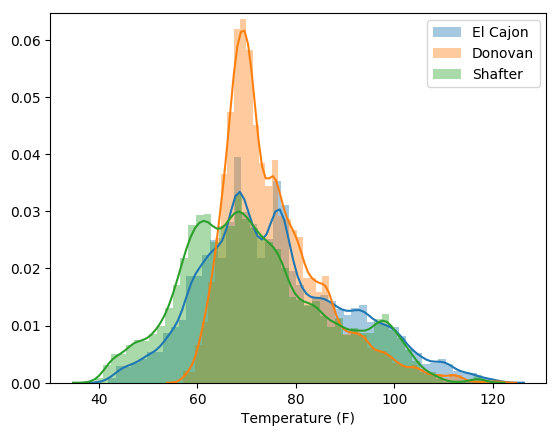
\includegraphics[width=0.5\textwidth]{results/distributions/temperature.png}
\caption{Temperature distribution based on
location}
\label{fig:temperature}
\end{figure}

\begin{figure}[H]
\centering
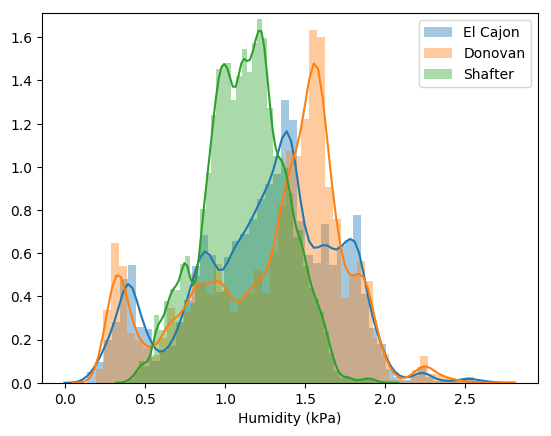
\includegraphics[width=0.5\textwidth]{results/distributions/humidity.png}
\caption{Absolute humidity distribution based on
location}
\label{fig:humidity}
\end{figure}

\begin{figure}[H]
\centering
\begin{subfigure}{0.32\textwidth}
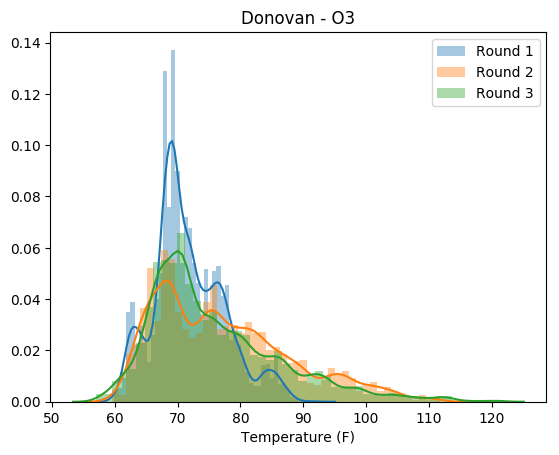
\includegraphics[width=\textwidth]{results/distributions/location_donovan_temperature.png}
\caption{Donovan}
\end{subfigure}
\begin{subfigure}{0.32\textwidth}
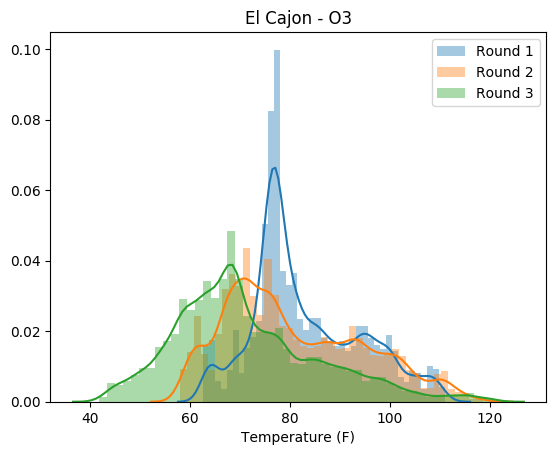
\includegraphics[width=\textwidth]{results/distributions/location_elcajon_temperature.png}
\caption{El Cajon}
\end{subfigure}
\begin{subfigure}{0.32\textwidth}
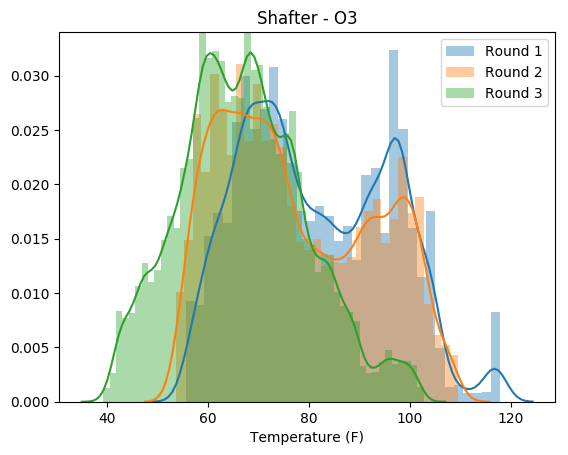
\includegraphics[width=\textwidth]{results/distributions/location_shafter_temperature.png}
\caption{Shafter}
\end{subfigure}
\caption{Temperature at locations}
\label{fig:temperature-locations}
\end{figure}

\begin{figure}[H]
\centering
\begin{subfigure}{0.32\textwidth}
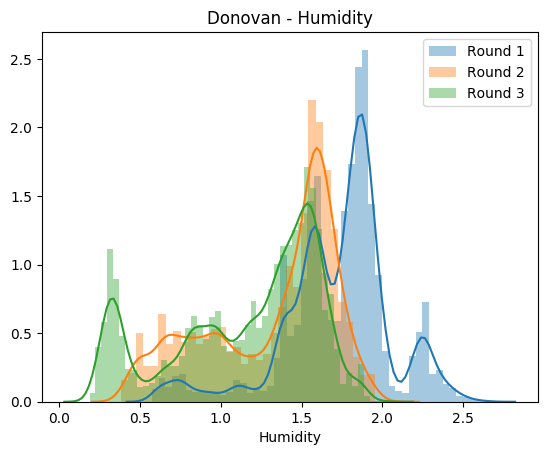
\includegraphics[width=\textwidth]{results/distributions/location_donovan_humidity.png}
\caption{Donovan}
\end{subfigure}
\begin{subfigure}{0.32\textwidth}
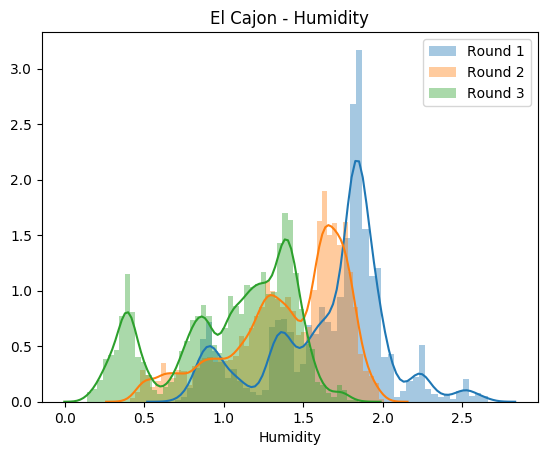
\includegraphics[width=\textwidth]{results/distributions/location_elcajon_humidity.png}
\caption{El Cajon}
\end{subfigure}
\begin{subfigure}{0.32\textwidth}
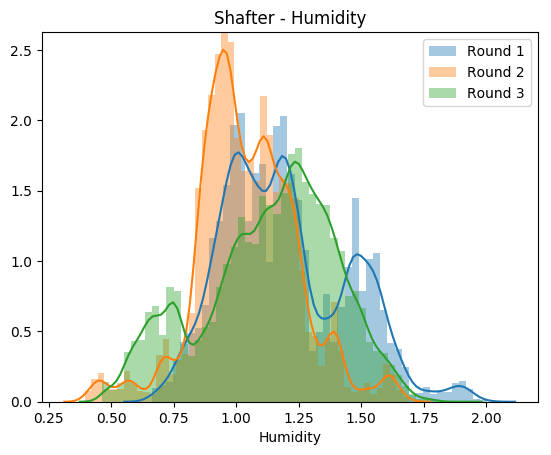
\includegraphics[width=\textwidth]{results/distributions/location_shafter_humidity.png}
\caption{Shafter}
\end{subfigure}
\caption{Absolute humidity at locations}
\label{fig:humidity-locations}
\end{figure}

\fi

\begin{figure}[H]
\centering
\begin{subfigure}{0.32\textwidth}
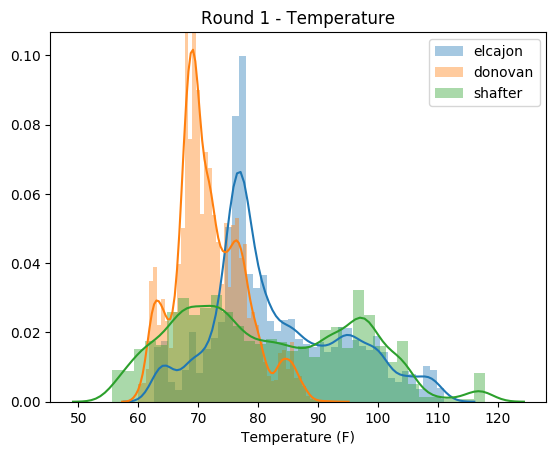
\includegraphics[width=\textwidth]{results/distributions/round1_temperature.png}
\caption{Round 1}
\end{subfigure}
\begin{subfigure}{0.32\textwidth}
.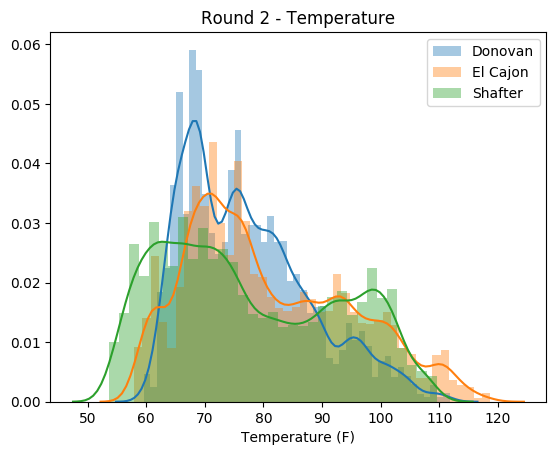
\includegraphics[width=\textwidth]{results/distributions/round2_temperature.png}
\caption{Round 2}
\end{subfigure}
\begin{subfigure}{0.32\textwidth}
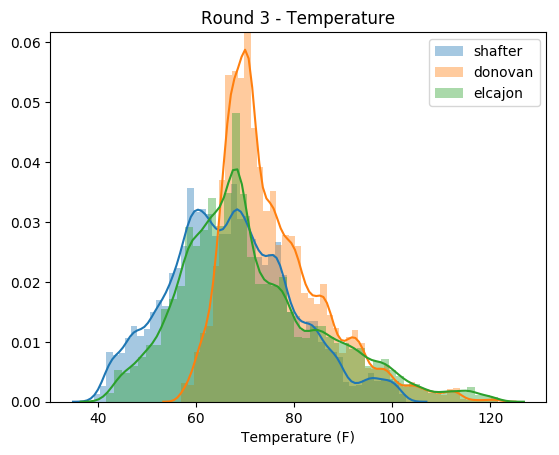
\includegraphics[width=\textwidth]{results/distributions/round3_temperature.png}
\caption{Round 3}
\end{subfigure}
\caption{Temperature distributions for each location, by round.}
\label{fig:temperature-rounds}
\end{figure}

\begin{figure}[H]
\centering
\begin{subfigure}{0.32\textwidth}
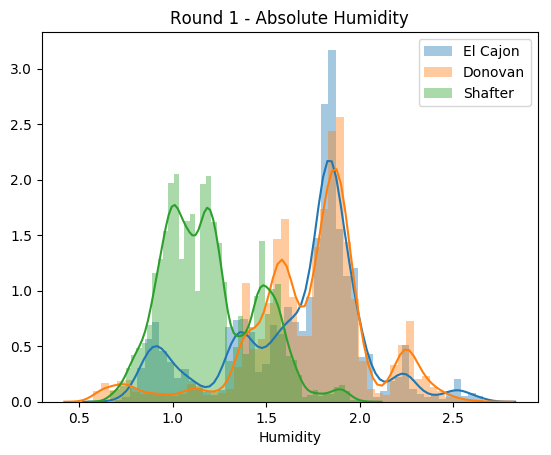
\includegraphics[width=\textwidth]{results/distributions/round1_humidity.png}
\caption{Round 1}
\end{subfigure}
\begin{subfigure}{0.32\textwidth}
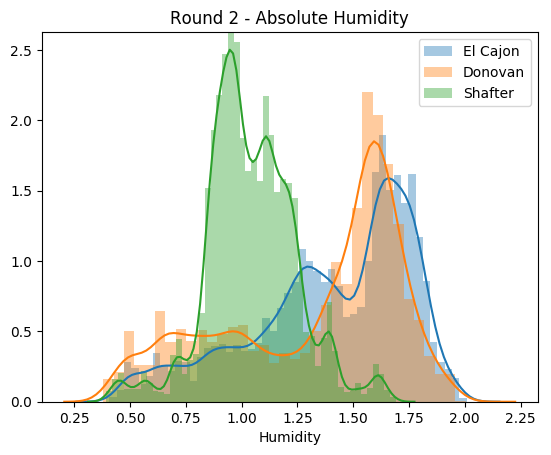
\includegraphics[width=\textwidth]{results/distributions/round2_humidity.png}
\caption{Round 2}
\end{subfigure}
\begin{subfigure}{0.32\textwidth}
\includegraphics[width=\textwidth]{results/distributions/round3_humidity.png}
\caption{Round 3}
\end{subfigure}
\caption{Humidity distributions for each location, by round.}
\label{fig:humidity-rounds}
\end{figure}


%\subsection{Pollutant values}

\iffalse

\begin{figure}[H]
\centering
\begin{subfigure}{0.32\textwidth}
\includegraphics[width=\textwidth]{results/distributions/location_donovan_no2.png}
\caption{Donovan}
\end{subfigure}
\begin{subfigure}{0.32\textwidth}
\includegraphics[width=\textwidth]{results/distributions/location_elcajon_no2.png}
\caption{El Cajon}
\end{subfigure}
\begin{subfigure}{0.32\textwidth}
\includegraphics[width=\textwidth]{results/distributions/location_shafter_no2.png}
\caption{Shafter}
\end{subfigure}
\caption{NO\textus{2} at locations}
\label{fig:no2-locations}
\end{figure}

\fi

\begin{figure}[H]
\centering
\begin{subfigure}{0.32\textwidth}
\includegraphics[width=\textwidth]{results/distributions/round1_no2.png}
\caption{Round 1}
\end{subfigure}
\begin{subfigure}{0.32\textwidth}
\includegraphics[width=\textwidth]{results/distributions/round2_no2.png}
\caption{Round 2}
\end{subfigure}
\begin{subfigure}{0.32\textwidth}
\includegraphics[width=\textwidth]{results/distributions/round3_no2.png}
\caption{Round 3}
\end{subfigure}
\caption{NO\textus{2} distributions for each location, by round.}
\label{fig:no2-rounds}
\end{figure}

\iffalse

\begin{figure}[H]
\centering
\begin{subfigure}{0.32\textwidth}
\includegraphics[width=\textwidth]{results/distributions/location_donovan_o3.png}
\caption{Round 1}
\end{subfigure}
\begin{subfigure}{0.32\textwidth}
\includegraphics[width=\textwidth]{results/distributions/location_elcajon_o3.png}
\caption{Round 2}
\end{subfigure}
\begin{subfigure}{0.32\textwidth}
\includegraphics[width=\textwidth]{results/distributions/location_shafter_o3.png}
\caption{Round 3}
\end{subfigure}
\caption{O\textus{3} at locations}
\label{fig:o3-locations}
\end{figure}

\fi

\begin{figure}[H]
\centering
\begin{subfigure}{0.32\textwidth}
\includegraphics[width=\textwidth]{results/distributions/round1_o3.png}
\caption{Round 1}
\end{subfigure}
\begin{subfigure}{0.32\textwidth}
\includegraphics[width=\textwidth]{results/distributions/round2_o3.png}
\caption{Round 2}
\end{subfigure}
\begin{subfigure}{0.32\textwidth}
\includegraphics[width=\textwidth]{results/distributions/round3_o3.png}
\caption{Round 3}
\end{subfigure}
\caption{O\textus{3} distributions for each location, by round.}
\label{fig:o3-rounds}
\end{figure}

\section{Additional Error Density Plots}\label{sec:remaining-error-density-plots}

\begin{figure}[H]
\centering
\begin{subfigure}{0.33\textwidth}
\includegraphics[width=\textwidth]{\baselinedir/linear/error_density_temperature_donovan_O3.png}
\caption{LR, trained at Donovan}
\end{subfigure}
\begin{subfigure}{0.33\textwidth}
\includegraphics[width=\textwidth]{\baselinedir/linear/error_density_temperature_elcajon_O3.png}
\caption{LR, trained at El Cajon}
\end{subfigure}
\begin{subfigure}{0.33\textwidth}
\includegraphics[width=\textwidth]{\baselinedir/linear/error_density_temperature_shafter_O3.png}
\caption{LR, trained at Shafter}
\end{subfigure}
\begin{subfigure}{0.33\textwidth}
\includegraphics[width=\textwidth]{\baselinedir/subu/error_density_temperature_donovan_O3.png}
\caption{RF, trained at Donovan}
\end{subfigure}
\begin{subfigure}{0.33\textwidth}
\includegraphics[width=\textwidth]{\baselinedir/subu/error_density_temperature_elcajon_O3.png}
\caption{RF, trained at El Cajon}
\end{subfigure}
\begin{subfigure}{0.33\textwidth}
\includegraphics[width=\textwidth]{\baselinedir/subu/error_density_temperature_shafter_O3.png}
\caption{RF, trained at Shafter}
\end{subfigure}
\caption{Error density plots for O\textus{3} versus temperature for both Linear Regression (LR) and Random Forest (RF) in a Level 1 benchmark.}
\label{fig:error-density-O3-temp}
\end{figure}


\begin{figure}[H]
\centering
\begin{subfigure}{0.33\textwidth}
\includegraphics[width=\textwidth]{\baselinedir/linear/error_density_absolute-humidity_donovan_NO2.png}
\caption{LR, trained at Donovan}
\end{subfigure}
\begin{subfigure}{0.33\textwidth}
\includegraphics[width=\textwidth]{\baselinedir/linear/error_density_absolute-humidity_elcajon_NO2.png}
\caption{LR, trained at El Cajon}
\end{subfigure}
\begin{subfigure}{0.33\textwidth}
\includegraphics[width=\textwidth]{\baselinedir/linear/error_density_absolute-humidity_shafter_NO2.png}
\caption{LR, trained at Shafter}
\end{subfigure}
\begin{subfigure}{0.33\textwidth}
\includegraphics[width=\textwidth]{\baselinedir/subu/error_density_absolute-humidity_donovan_NO2.png}
\caption{RF, trained at Donovan}
\end{subfigure}
\begin{subfigure}{0.33\textwidth}
\includegraphics[width=\textwidth]{\baselinedir/subu/error_density_absolute-humidity_elcajon_NO2.png}
\caption{RF, trained at El Cajon}
\end{subfigure}
\begin{subfigure}{0.33\textwidth}
\includegraphics[width=\textwidth]{\baselinedir/subu/error_density_absolute-humidity_shafter_NO2.png}
\caption{RF, trained at Shafter}
\end{subfigure}
\caption{Error density plots for NO\textus{2} versus absolute humidity for both Linear Regression (LR) and Random Forest (RF) in a Level 1 benchmark.}
\label{fig:error-density-NO2-humidity}
\end{figure}

\begin{figure}[H]
\centering
\begin{subfigure}{0.33\textwidth}
\includegraphics[width=\textwidth]{\baselinedir/linear/error_density_absolute-humidity_donovan_NO2.png}
\caption{LR, trained at Donovan}
\end{subfigure}
\begin{subfigure}{0.33\textwidth}
\includegraphics[width=\textwidth]{\baselinedir/linear/error_density_absolute-humidity_elcajon_NO2.png}
\caption{LR, trained at El Cajon}
\end{subfigure}
\begin{subfigure}{0.33\textwidth}
\includegraphics[width=\textwidth]{\baselinedir/linear/error_density_absolute-humidity_shafter_NO2.png}
\caption{LR, trained at Shafter}
\end{subfigure}
\begin{subfigure}{0.33\textwidth}
\includegraphics[width=\textwidth]{\baselinedir/subu/error_density_absolute-humidity_donovan_NO2.png}
\caption{RF, trained at Donovan}
\end{subfigure}
\begin{subfigure}{0.33\textwidth}
\includegraphics[width=\textwidth]{\baselinedir/subu/error_density_absolute-humidity_elcajon_NO2.png}
\caption{RF, trained at El Cajon}
\end{subfigure}
\begin{subfigure}{0.33\textwidth}
\includegraphics[width=\textwidth]{\baselinedir/subu/error_density_absolute-humidity_shafter_NO2.png}
\caption{RF, trained at Shafter}
\end{subfigure}
\caption{Error density plots for NO\textus{2} versus absolute-humidity for both Linear Regression (LR) and Random Forest (RF) in a Level 1 benchmark.}
\label{fig:error-density-NO2-temp}
\end{figure}

\iffalse
\section{Basic calibration results}

A calibration model takes in sensor readings and environment
variables and outputs pollutant levels. In this basic setup,
we train a model for each board.
We aim to train models that are robust after moving location.

\begin{table}[H]
\centering
\begin{tabular}{|l|l|}
\hline
\textbf{Level 0} & Train on location A and test on location A \\ \hline
\textbf{Level 1} & Train on location A and test on location B \\ \hline
\textbf{Level 2} & Train on location A and B and test on location C \\ \hline
\textbf{Level 3} & Train on location A, B, and C and test on location A \\ \hline
\end{tabular}
\caption{Description of different types of benchmarks.}
\label{tab:levels}
\end{table}

We benchmark four different models: linear regression (linear), random forest regressors based on \citep{Zimmerman2018},
a 2-layer neural network (NN[2]), and a 4-layer neural network (NN[4]). The ideal model will
both predict pollutant levels accurately and
generalize across locations.

To benchmark, we first take our data sets (25 total, see \autoref{tab:board-rotations}), and partition each into training and testing sets (20\% reserved for testing).
We perform several types of benchmarks,
each to learn about the transferrability of each model (see \autoref{tab:levels}).
In general, we expect Level 0 and Level 3 performance to be the best, as they involve training and testing on data from the same distribution. Furthermore, we expected Level 2 to have lower error than Level 1, because Level 2 is trained on more data and a wider distribution of data (two locations vs one location).
If a model's Level 1 and Level 2 error are close to Level 0 and Level 3, then the model transfers well. Otherwise, the model overfits to its location.


These raw results are in \autoref{sec:simpleresults}. 
We split results into training vs. testing
results, where we expect train performance
to be better than test.
Overall, we see that random forests have the lowest Level 0 and Level 3 error. This is consistent with results we see in \citet{Zimmerman2018}. 
We observe when comparing Level 1 error difference (Level 1 train minus Level 1 test), random forests suffer great
drops in performance.
This hints that RFs are overfitting to the training data, even if they
report the lowest test error for Level 0 and Level 3.  See \autoref{fig:generalization} for 
details.

\begin{figure}[H]
\centering
\begin{subfigure}{0.45\textwidth}
\includegraphics[width=\textwidth]{\baselinedir/NO2" "MAE_difference.png}
\caption{NO\textus{2}}
\end{subfigure}
\begin{subfigure}{0.45\textwidth}
\includegraphics[width=\textwidth]{\baselinedir/O3" "MAE_difference.png}
\caption{O\textus{3}}
\end{subfigure}
\caption{Difference plots. Train minus test errors for various models. A smaller value means that the models transfer better.}
\label{fig:generalization}
\end{figure}

\section{Neural representation learning}

We now present split-neural network results: we split
up calibration into two stages, a sensor model
and a pollutant model, which we will call $s_i$ and $c$
respectively.
Given a sensor readings $x$ from board $i$,
and environment readings $e$
we obtain a calibrated reading $y$ by simply passing it through
the sensor model, then the pollutant model, i.e.
\begin{align*}
    y = c(s_i(x), e)
\end{align*}
We can learn individual sensor models for each board,
but the pollutant model is shared across boards. This allows
us to pool data across boards to learn the pollutant model.
Furthermore, environment variables are only 
included in the pollutant model, which hopefully enables
a stronger fit with a very complex pollutant model.

Each $s_i(x)$ outputs a ``sensor representation'', which is chosen
to be some fixed dimension $d$. We hope that the sensor representation
contains the minimal information to produce calibrated readings.

We experiment with each $s_i$ being a linear regression model,
and $c$ being a deep neural network (two layers, 100 width ReLU). 
Each set of data we collect
is identified by a triplet of information (round, location, board number). In total, we have 25 of such data sets as defined in \autoref{tab:board-rotations}. To benchmark these split models, we train on all of these data sets, but
hold one triple out, resulting in a
total training set size of 24 data sets and test size of 1 data set. This results in a total of 25 experiments
for which we boxplot the results.
We compare the split models to our four static models (Linear, NN[2], NN[4], Random Forest) by comparing the split-NN performance on the held out data set to the Level 2 performance of the four models.
Level 2 performance corresponds to training on two locations
and testing on the third. The split model has access to the same training data as the Level 2 models, but with the addition of data from other boards. The hope is this additional board data can help improve upon Level 2 performance, which can be thought of as the ``best'' possible transfer performance.

\begin{figure}[H]
\begin{subfigure}{0.49\textwidth}
\includegraphics[width=\textwidth]{\splitdir/linear/no2mae.png}
\caption{NO\textus{2} MAE}
\end{subfigure}
\begin{subfigure}{0.49\textwidth}
\includegraphics[width=\textwidth]{\splitdir/linear/o3mae.png}
\caption{O\textus{3} MAE}
\end{subfigure}
\begin{subfigure}{0.49\textwidth}
\includegraphics[width=\textwidth]{\splitdir/linear/no2cvmae.png}
\caption{NO\textus{2} CvMAE}
\end{subfigure}
\begin{subfigure}{0.49\textwidth}
\includegraphics[width=\textwidth]{\splitdir/linear/o3cvmae.png}
\caption{O\textus{3} CvMAE}
\end{subfigure}
\caption{Comparison of errors of split-NN and Linear. Training size corresponds to a Level 1 or Level 2 comparison.}
\end{figure}

\begin{figure}[H]
\begin{subfigure}{0.49\textwidth}
\includegraphics[width=\textwidth]{\splitdir/nn-2/no2mae.png}
\caption{NO\textus{2} MAE}
\end{subfigure}
\begin{subfigure}{0.49\textwidth}
\includegraphics[width=\textwidth]{\splitdir/nn-2/o3mae.png}
\caption{O\textus{3} MAE}
\end{subfigure}
\begin{subfigure}{0.49\textwidth}
\includegraphics[width=\textwidth]{\splitdir/nn-2/no2cvmae.png}
\caption{NO\textus{2} CvMAE}
\end{subfigure}
\begin{subfigure}{0.49\textwidth}
\includegraphics[width=\textwidth]{\splitdir/nn-2/o3cvmae.png}
\caption{O\textus{3} CvMAE}
\end{subfigure}
\caption{Comparison of errors of split-NN and NN[2]. Training size corresponds to a Level 1 or Level 2 comparison.}
\end{figure}

\begin{figure}[H]
\begin{subfigure}{0.49\textwidth}
\includegraphics[width=\textwidth]{\splitdir/nn-4/no2mae.png}
\caption{NO\textus{2} MAE}
\end{subfigure}
\begin{subfigure}{0.49\textwidth}
\includegraphics[width=\textwidth]{\splitdir/nn-4/o3mae.png}
\caption{O\textus{3} MAE}
\end{subfigure}
\begin{subfigure}{0.49\textwidth}
\includegraphics[width=\textwidth]{\splitdir/nn-4/no2cvmae.png}
\caption{NO\textus{2} CvMAE}
\end{subfigure}
\begin{subfigure}{0.49\textwidth}
\includegraphics[width=\textwidth]{\splitdir/nn-4/o3cvmae.png}
\caption{O\textus{3} CvMAE}
\end{subfigure}
\caption{Comparison of errors of split-NN and NN[4]. Training size corresponds to a Level 1 or Level 2 comparison.}
\end{figure}

\begin{figure}[H]
\begin{subfigure}{0.49\textwidth}
\includegraphics[width=\textwidth]{\splitdir/subu/no2mae.png}
\caption{NO\textus{2} MAE}
\end{subfigure}
\begin{subfigure}{0.49\textwidth}
\includegraphics[width=\textwidth]{\splitdir/subu/o3mae.png}
\caption{O\textus{3} MAE}
\end{subfigure}
\begin{subfigure}{0.49\textwidth}
\includegraphics[width=\textwidth]{\splitdir/subu/no2cvmae.png}
\caption{NO\textus{2} CvMAE}
\end{subfigure}
\begin{subfigure}{0.49\textwidth}
\includegraphics[width=\textwidth]{\splitdir/subu/o3cvmae.png}
\caption{O\textus{3} CvMAE}
\end{subfigure}
\caption{Comparison of errors of split-NN and random forest. Training size corresponds to a Level 1 or Level 2 comparison.}
\end{figure}

To further accentuate the improvement, we can compare
the difference in performance between split-NN and the four models. In these plots, a more negative value corresponds to a larger improvement.

\begin{figure}[H]
\begin{subfigure}{0.49\textwidth}
\includegraphics[width=\textwidth]{\splitdir/linear/no2mae-diff.png}
\caption{NO\textus{2} MAE Improvement}
\end{subfigure}
\begin{subfigure}{0.49\textwidth}
\includegraphics[width=\textwidth]{\splitdir/linear/o3mae-diff.png}
\caption{O\textus{3} MAE Improvement}
\end{subfigure}
\begin{subfigure}{0.49\textwidth}
\includegraphics[width=\textwidth]{\splitdir/linear/no2cvmae-diff.png}
\caption{NO\textus{2} CvMAE Improvement}
\end{subfigure}
\begin{subfigure}{0.49\textwidth}
\includegraphics[width=\textwidth]{\splitdir/linear/o3cvmae-diff.png}
\caption{O\textus{3} CvMAE Improvement}
\end{subfigure}
\caption{Comparison of errors of split-NN and Linear.}
\end{figure}

\begin{figure}[H]
\begin{subfigure}{0.49\textwidth}
\includegraphics[width=\textwidth]{\splitdir/nn-2/no2mae-diff.png}
\caption{NO\textus{2} MAE Improvement}
\end{subfigure}
\begin{subfigure}{0.49\textwidth}
\includegraphics[width=\textwidth]{\splitdir/nn-2/o3mae-diff.png}
\caption{O\textus{3} MAE Improvement}
\end{subfigure}
\begin{subfigure}{0.49\textwidth}
\includegraphics[width=\textwidth]{\splitdir/nn-2/no2cvmae-diff.png}
\caption{NO\textus{2} CvMAE Improvement}
\end{subfigure}
\begin{subfigure}{0.49\textwidth}
\includegraphics[width=\textwidth]{\splitdir/nn-2/o3cvmae-diff.png}
\caption{O\textus{3} CvMAE Improvement}
\end{subfigure}
\caption{Comparison of errors of split-NN and NN[2].}
\end{figure}

\begin{figure}[H]
\begin{subfigure}{0.49\textwidth}
\includegraphics[width=\textwidth]{\splitdir/nn-4/no2mae-diff.png}
\caption{NO\textus{2} MAE Improvement}
\end{subfigure}
\begin{subfigure}{0.49\textwidth}
\includegraphics[width=\textwidth]{\splitdir/nn-4/o3mae-diff.png}
\caption{O\textus{3} MAE Improvement}
\end{subfigure}
\begin{subfigure}{0.49\textwidth}
\includegraphics[width=\textwidth]{\splitdir/nn-4/no2cvmae-diff.png}
\caption{NO\textus{2} CvMAE Improvement}
\end{subfigure}
\begin{subfigure}{0.49\textwidth}
\includegraphics[width=\textwidth]{\splitdir/nn-4/o3cvmae-diff.png}
\caption{O\textus{3} CvMAE Improvement}
\end{subfigure}
\caption{Comparison of errors of split-NN and NN[4].}
\end{figure}

\begin{figure}[H]
\begin{subfigure}{0.49\textwidth}
\includegraphics[width=\textwidth]{\splitdir/subu/no2mae-diff.png}
\caption{NO\textus{2} MAE Improvement}
\end{subfigure}
\begin{subfigure}{0.49\textwidth}
\includegraphics[width=\textwidth]{\splitdir/subu/o3mae-diff.png}
\caption{O\textus{3} MAE Improvement}
\end{subfigure}
\begin{subfigure}{0.49\textwidth}
\includegraphics[width=\textwidth]{\splitdir/subu/no2cvmae-diff.png}
\caption{NO\textus{2} CvMAE Improvement}
\end{subfigure}
\begin{subfigure}{0.49\textwidth}
\includegraphics[width=\textwidth]{\splitdir/subu/o3cvmae-diff.png}
\caption{O\textus{3} CvMAE Improvement}
\end{subfigure}
\caption{Comparison of errors of split-NN and random forest.}
\end{figure}

\fi

\renewcommand{\thetable}{\Alph{section}.\arabic{table}}

\section{Summaries of Data for each Location and Round}
\label{sec:summaryresults}

\begin{table}[H]
\scriptsize
\begin{tabular}{llrrrrr}
\toprule
        &       &        epa-no2 &         epa-o3 &    temperature &       pressure &       humidity \\
Location & {} &                &                &                &                &                \\
\midrule
donovan & count &  100788.000000 &  100788.000000 &  100788.000000 &  100788.000000 &  100788.000000 \\
        & mean &      10.434149 &      33.742201 &      24.169544 &     991.767126 &      45.937553 \\
        & std &      10.806435 &      15.377371 &       5.623704 &       3.225557 &      21.965513 \\
        & min &       0.000000 &       0.000000 &      13.900000 &     982.820000 &       4.086000 \\
        & 25\% &       3.000000 &      24.000000 &      20.100000 &     989.530000 &      27.245000 \\
        & 50\% &       7.000000 &      35.000000 &      22.620000 &     991.460000 &      49.513000 \\
        & 75\% &      14.000000 &      43.000000 &      27.000000 &     993.610000 &      64.396000 \\
        & max &     157.000000 &      96.000000 &      49.710000 &    1004.160000 &      92.753000 \\
elcajon & count &   97412.000000 &   97412.000000 &   97412.000000 &   97412.000000 &   97412.000000 \\
        & mean &      12.914015 &      29.331499 &      24.341702 &     997.287606 &      43.923309 \\
        & std &       9.732012 &      19.337040 &       8.232391 &       3.507203 &      20.076611 \\
        & min &       0.000000 &       1.000000 &       5.430000 &     989.230000 &       2.733000 \\
        & 25\% &       5.000000 &      11.000000 &      18.570000 &     994.880000 &      28.623000 \\
        & 50\% &      10.000000 &      31.000000 &      23.380000 &     996.890000 &      45.052500 \\
        & 75\% &      20.000000 &      43.000000 &      29.700000 &     999.450000 &      61.166250 \\
        & max &      66.000000 &      95.000000 &      49.790000 &    1010.480000 &      85.827000 \\
shafter & count &  119785.000000 &  119785.000000 &  119785.000000 &  119785.000000 &  119785.000000 \\
        & mean &      12.578259 &      26.357091 &      22.100842 &    1003.882723 &      45.804388 \\
        & std &       9.078981 &      20.739128 &       8.184091 &       5.595797 &      18.072375 \\
        & min &       0.000000 &       0.000000 &       4.010000 &     872.755556 &       6.349000 \\
        & 25\% &       4.700000 &       7.800000 &      16.155556 &     999.750000 &      30.585000 \\
        & 50\% &      10.800000 &      22.300000 &      21.040000 &    1003.990000 &      46.763000 \\
        & 75\% &      19.000000 &      41.200000 &      27.200000 &    1007.400000 &      60.965000 \\
        & max &     594.600000 &     110.400000 &      47.700000 &    1019.580000 &      85.047000 \\
\bottomrule
\end{tabular}

\caption{Summary of data set grouped by location}
\label{tab:locationsummary}
\end{table}

\begin{table}[H]
\scriptsize
\begin{tabular}{llrrrrr}
\toprule
  &       &        epa-no2 &         epa-o3 &    temperature &       pressure &       humidity \\
Round & {} &                &                &                &                &                \\
\midrule
1 & count &   49779.000000 &   49779.000000 &   49779.000000 &   49779.000000 &   49779.000000 \\
  & mean &       5.510173 &      36.010330 &      26.061407 &     994.458473 &      48.324276 \\
  & std &       5.472665 &      13.867920 &       6.776587 &       4.786306 &      19.538803 \\
  & min &       0.000000 &       1.300000 &      13.100000 &     872.755556 &       9.644000 \\
  & 25\% &       2.000000 &      28.000000 &      20.900000 &     990.920000 &      31.793000 \\
  & 50\% &       3.700000 &      37.300000 &      24.600000 &     995.240000 &      50.513000 \\
  & 75\% &       6.600000 &      45.000000 &      30.130000 &     997.640000 &      61.526500 \\
  & max &      57.000000 &     110.400000 &      47.700000 &    1002.940000 &      92.753000 \\
2 & count &   75129.000000 &   75129.000000 &   75129.000000 &   75129.000000 &   75129.000000 \\
  & mean &      11.915875 &      36.973669 &      25.952835 &     995.989062 &      41.511134 \\
  & std &       9.583090 &      21.259456 &       7.576508 &       6.074511 &      19.756994 \\
  & min &      -1.000000 &      -2.400000 &      12.000000 &     982.820000 &       4.420000 \\
  & 25\% &       5.000000 &      19.200000 &      20.000000 &     990.990000 &      23.461000 \\
  & 50\% &       8.000000 &      36.000000 &      24.400000 &     995.420000 &      41.539000 \\
  & 75\% &      17.900000 &      53.000000 &      31.710000 &    1000.710000 &      56.961000 \\
  & max &      82.000000 &      96.000000 &      48.180000 &    1009.890000 &      87.562000 \\
3 & count &  193077.000000 &  193077.000000 &  193077.000000 &  193077.000000 &  193077.000000 \\
  & mean &      13.708376 &      25.092386 &      21.791316 &     999.732162 &      45.945741 \\
  & std &      10.225285 &      17.803517 &       7.275538 &       6.707979 &      20.012530 \\
  & min &      -3.000000 &      -6.200000 &       4.010000 &     986.770000 &       2.733000 \\
  & 25\% &       5.100000 &       8.000000 &      17.190000 &     994.300000 &      30.192000 \\
  & 50\% &      11.600000 &      24.700000 &      21.000000 &     999.090000 &      48.470000 \\
  & 75\% &      20.000000 &      38.500000 &      25.780000 &    1004.690000 &      63.450000 \\
  & max &     594.600000 &      87.900000 &      49.790000 &    1019.580000 &      85.440000 \\
\bottomrule
\end{tabular}

\caption{Summary of data set grouped by round}
\label{tab:roundsummary}
\end{table}

\section{Raw Results for Baseline Calibration Models}
\label{sec:simpleresults}
The following the complete error results for the trained models across the various conditions.  In these tables, the modeling methods are labeled as MLR for multiple linear regression, NN-2 for 2-layer neural network, NN-4 for 4-layer neural network, and RF for random forest, as described in Section~\ref{sec:calibration-methods}.  Likewise, the error measures are labeled as MAE for mean absolute error, CvMAE for coefficient of variation of the mean absolute error, MBE for mean bias error, MSE for mean standard error, R\textasciicircum2 is the coefficient of determination, crMSE for centered root mean square error, and rMSE for root mean squared error.  The results are disaggregated by test and train sites, and averaged across the sensor packages.

\begin{table}[h]
\begin{tabular}{llrrrrrrr}
\toprule
 Train Site & Method &   MAE &  CvMAE &       MBE &     MSE &   R\textasciicircum2 &  crMSE &   rMSE \\
\midrule
elcajon & MLR & 3.860 & 0.256 & 1.163e-14 & 28.094 & 0.685 & 5.259 & 5.259\\
donovan & MLR & 5.520 & 0.567 & 1.528e-15 & 73.035 & 0.312 & 8.374 & 8.374\\
shafter & MLR & 4.671 & 0.354 & 3.628e-15 & 40.945 & 0.492 & 6.380 & 6.380\\
elcajon & NN-2 & 2.003 & 0.135 & 0.127 & 8.137 & 0.905 & 2.831 & 2.844\\
donovan & NN-2 & 3.134 & 0.328 & 0.093 & 27.100 & 0.733 & 5.175 & 5.189\\
shafter & NN-2 & 2.648 & 0.200 & 0.051 & 17.439 & 0.787 & 4.131 & 4.135\\
elcajon & NN-4 & 1.109 & 0.074 & 0.076 & 2.976 & 0.967 & 1.700 & 1.704\\
donovan & NN-4 & 1.946 & 0.213 & 0.033 & 13.955 & 0.835 & 3.527 & 3.548\\
shafter & NN-4 & 1.755 & 0.133 & -0.054 & 8.541 & 0.895 & 2.868 & 2.872\\
elcajon & RF & 0.477 & 0.032 & -0.011 & 0.673 & 0.993 & 0.808 & 0.808\\
donovan & RF & 0.999 & 0.112 & -0.022 & 3.705 & 0.956 & 1.870 & 1.871\\
shafter & RF & 0.514 & 0.039 & -0.016 & 1.513 & 0.981 & 1.193 & 1.193\\
\bottomrule
\end{tabular}
\caption{Level 0 train results for NO2 (train and test on the same data set).}
\end{table}

\begin{table}[h]
\begin{tabular}{lllrrrrrrr}
\toprule
 Train Site & Test Site & Method &   MAE &  CvMAE &       MBE &     MSE &   R\textasciicircum2 &  crMSE &   rMSE \\
\midrule
elcajon & elcajon & MLR & 3.869 & 0.256 & 0.015 & 28.999 & 0.683 & 5.333 & 5.333\\
donovan & donovan & MLR & 5.573 & 0.556 & 0.160 & 75.037 & 0.315 & 8.504 & 8.512\\
shafter & shafter & MLR & 4.671 & 0.353 & 0.004 & 38.467 & 0.511 & 6.191 & 6.191\\
elcajon & elcajon & NN-2 & 2.074 & 0.140 & 0.127 & 9.185 & 0.895 & 3.006 & 3.018\\
donovan & donovan & NN-2 & 3.390 & 0.345 & 0.204 & 31.458 & 0.696 & 5.559 & 5.581\\
shafter & shafter & NN-2 & 2.694 & 0.203 & 0.052 & 15.772 & 0.802 & 3.942 & 3.946\\
elcajon & elcajon & NN-4 & 1.465 & 0.098 & 0.076 & 5.524 & 0.938 & 2.327 & 2.331\\
donovan & donovan & NN-4 & 2.739 & 0.288 & 0.105 & 24.875 & 0.729 & 4.907 & 4.924\\
shafter & shafter & NN-4 & 2.089 & 0.158 & -0.060 & 10.702 & 0.865 & 3.252 & 3.256\\
elcajon & elcajon & RF & 0.972 & 0.064 & -0.028 & 2.929 & 0.968 & 1.683 & 1.683\\
donovan & donovan & RF & 2.010 & 0.216 & 0.031 & 15.113 & 0.830 & 3.794 & 3.797\\
shafter & shafter & RF & 1.028 & 0.078 & -0.041 & 3.822 & 0.951 & 1.943 & 1.943\\
\bottomrule
\end{tabular}
\caption{Level 0 test results for NO2.}
\end{table}

\begin{table}[h]
\begin{tabular}{llrrrrrrr}
\toprule
 Train Site & Method &   MAE &  CvMAE &       MBE &     MSE &   R\textasciicircum2 &  crMSE &   rMSE \\
\midrule
elcajon & MLR & 6.010 & 0.245 & 1.647e-14 & 60.276 & 0.827 & 7.666 & 7.666\\
donovan & MLR & 6.916 & 0.193 & -1.881e-15 & 85.486 & 0.584 & 9.131 & 9.131\\
shafter & MLR & 5.882 & 0.239 & 9.460e-15 & 63.567 & 0.841 & 7.877 & 7.877\\
elcajon & NN-2 & 2.810 & 0.112 & -0.150 & 16.200 & 0.954 & 3.940 & 3.947\\
donovan & NN-2 & 4.237 & 0.117 & -0.270 & 35.055 & 0.821 & 5.824 & 5.855\\
shafter & NN-2 & 3.498 & 0.141 & 0.013 & 24.929 & 0.939 & 4.895 & 4.909\\
elcajon & NN-4 & 1.369 & 0.055 & -0.092 & 4.418 & 0.987 & 2.053 & 2.064\\
donovan & NN-4 & 2.781 & 0.077 & -0.212 & 21.314 & 0.874 & 4.055 & 4.102\\
shafter & NN-4 & 2.184 & 0.090 & 0.001 & 10.817 & 0.973 & 3.248 & 3.251\\
elcajon & RF & 0.598 & 0.024 & 0.006 & 0.962 & 0.997 & 0.976 & 0.976\\
donovan & RF & 1.341 & 0.037 & 0.014 & 4.938 & 0.971 & 1.988 & 1.988\\
shafter & RF & 0.643 & 0.027 & 0.011 & 1.176 & 0.997 & 1.083 & 1.083\\
\bottomrule
\end{tabular}
\caption{Level 0 train results for O3 (train and test on the same data set).}
\end{table}

\begin{table}[h]
\begin{tabular}{lllrrrrrrr}
\toprule
 Train Site & Test Site & Method &   MAE &  CvMAE &       MBE &     MSE &   R\textasciicircum2 &  crMSE &   rMSE \\
\midrule
elcajon & elcajon & MLR & 6.038 & 0.245 & 0.040 & 61.471 & 0.822 & 7.744 & 7.744\\
donovan & donovan & MLR & 6.931 & 0.195 & -0.255 & 85.324 & 0.604 & 9.116 & 9.124\\
shafter & shafter & MLR & 5.877 & 0.240 & 0.020 & 63.379 & 0.842 & 7.857 & 7.858\\
elcajon & elcajon & NN-2 & 2.919 & 0.115 & -0.133 & 17.626 & 0.950 & 4.113 & 4.118\\
donovan & donovan & NN-2 & 4.516 & 0.126 & -0.488 & 40.687 & 0.802 & 6.193 & 6.253\\
shafter & shafter & NN-2 & 3.568 & 0.145 & 0.020 & 26.052 & 0.937 & 4.999 & 5.011\\
elcajon & elcajon & NN-4 & 1.903 & 0.075 & -0.068 & 9.252 & 0.974 & 2.966 & 2.974\\
donovan & donovan & NN-4 & 3.830 & 0.107 & -0.330 & 33.794 & 0.825 & 5.399 & 5.456\\
shafter & shafter & NN-4 & 2.672 & 0.109 & -0.012 & 17.052 & 0.959 & 4.050 & 4.052\\
elcajon & elcajon & RF & 1.217 & 0.049 & 0.015 & 3.987 & 0.988 & 1.987 & 1.987\\
donovan & donovan & RF & 2.723 & 0.076 & -0.103 & 19.179 & 0.897 & 3.931 & 3.934\\
shafter & shafter & RF & 1.284 & 0.054 & 0.024 & 4.651 & 0.988 & 2.155 & 2.155\\
\bottomrule
\end{tabular}
\caption{Level 0 test results for O3.}
\end{table}


\begin{table}[h]
\begin{tabular}{llrrrrrrr}
\toprule
 Train Site & Method &   MAE &  CvMAE &       MBE &     MSE &   R\textasciicircum2 &  crMSE &   rMSE \\
\midrule
elcajon & MLR & 3.869 & 0.256 & 0.015 & 28.999 & 0.683 & 5.333 & 5.333\\
donovan & MLR & 5.573 & 0.556 & 0.160 & 75.037 & 0.315 & 8.504 & 8.512\\
shafter & MLR & 4.671 & 0.353 & 0.004 & 38.467 & 0.511 & 6.191 & 6.191\\
elcajon & NN-2 & 2.074 & 0.140 & 0.127 & 9.185 & 0.895 & 3.006 & 3.018\\
donovan & NN-2 & 3.390 & 0.345 & 0.204 & 31.458 & 0.696 & 5.559 & 5.581\\
shafter & NN-2 & 2.694 & 0.203 & 0.052 & 15.772 & 0.802 & 3.942 & 3.946\\
elcajon & NN-4 & 1.465 & 0.098 & 0.076 & 5.524 & 0.938 & 2.327 & 2.331\\
donovan & NN-4 & 2.739 & 0.288 & 0.105 & 24.875 & 0.729 & 4.907 & 4.924\\
shafter & NN-4 & 2.089 & 0.158 & -0.060 & 10.702 & 0.865 & 3.252 & 3.256\\
elcajon & RF & 0.972 & 0.064 & -0.028 & 2.929 & 0.968 & 1.683 & 1.683\\
donovan & RF & 2.010 & 0.216 & 0.031 & 15.113 & 0.830 & 3.794 & 3.797\\
shafter & RF & 1.028 & 0.078 & -0.041 & 3.822 & 0.951 & 1.943 & 1.943\\
\bottomrule
\end{tabular}
\caption{Level 1 train results for NO2 (train and test on the same data set).}
\end{table}

\begin{table}[h]
\begin{tabular}{lllrrrrrrr}
\toprule
 Train Site & Test Site & Method &   MAE &  CvMAE &       MBE &     MSE &   R\textasciicircum2 &  crMSE &   rMSE \\
\midrule
elcajon & donovan & MLR & 7.994 & 0.841 & -4.447 & 119.171 & -0.304 & 8.782 & 10.639\\
elcajon & shafter & MLR & 7.495 & 0.565 & -1.816 & 103.831 & -0.303 & 8.871 & 9.990\\
donovan & elcajon & MLR & 6.383 & 0.436 & 1.998 & 69.142 & 0.179 & 6.801 & 8.203\\
donovan & shafter & MLR & 8.860 & 0.676 & 0.639 & 132.238 & -0.711 & 8.201 & 11.351\\
shafter & elcajon & MLR & 7.472 & 0.504 & 1.940 & 115.789 & -0.303 & 9.532 & 10.366\\
shafter & donovan & MLR & 8.553 & 0.856 & 0.904 & 143.748 & -0.309 & 10.080 & 11.542\\
elcajon & donovan & NN-2 & 6.552 & 0.688 & -1.875 & 98.026 & -0.063 & 8.628 & 9.641\\
elcajon & shafter & NN-2 & 5.367 & 0.405 & -0.491 & 52.894 & 0.334 & 7.077 & 7.189\\
donovan & elcajon & NN-2 & 9.960 & 0.649 & 2.435 & 282.631 & -1.896 & 13.732 & 14.872\\
donovan & shafter & NN-2 & 8.567 & 0.662 & 2.822 & 173.652 & -1.359 & 10.145 & 11.805\\
shafter & elcajon & NN-2 & 9.623 & 0.642 & 3.077 & 269.781 & -2.158 & 13.186 & 14.291\\
shafter & donovan & NN-2 & 9.446 & 0.918 & 2.953 & 250.758 & -1.049 & 11.432 & 13.326\\
elcajon & donovan & NN-4 & 6.164 & 0.632 & -1.301 & 83.675 & 0.163 & 8.663 & 9.103\\
elcajon & shafter & NN-4 & 5.771 & 0.436 & -0.298 & 58.188 & 0.266 & 7.473 & 7.601\\
donovan & elcajon & NN-4 & 7.702 & 0.500 & -0.698 & 132.834 & -0.385 & 10.342 & 10.622\\
donovan & shafter & NN-4 & 7.947 & 0.614 & 1.850 & 148.190 & -0.995 & 10.032 & 10.690\\
shafter & elcajon & NN-4 & 8.609 & 0.563 & -0.022 & 156.109 & -0.689 & 11.210 & 11.768\\
shafter & donovan & NN-4 & 8.358 & 0.827 & -0.362 & 176.864 & -0.769 & 12.024 & 12.658\\
elcajon & donovan & RF & 5.813 & 0.598 & -1.477 & 72.216 & 0.291 & 8.005 & 8.414\\
elcajon & shafter & RF & 5.560 & 0.420 & -0.604 & 50.668 & 0.364 & 6.887 & 7.065\\
donovan & elcajon & RF & 5.904 & 0.384 & -1.458 & 61.572 & 0.346 & 7.186 & 7.597\\
donovan & shafter & RF & 6.579 & 0.505 & -1.846 & 79.515 & -0.048 & 7.700 & 8.645\\
shafter & elcajon & RF & 7.182 & 0.487 & -0.148 & 198.620 & -1.665 & 10.882 & 11.411\\
shafter & donovan & RF & 7.220 & 0.725 & -1.549 & 153.445 & -0.642 & 11.112 & 11.635\\
\bottomrule
\end{tabular}
\caption{Level 1 test results for NO2.}
\end{table}

\begin{table}[h]
\begin{tabular}{llrrrrrrr}
\toprule
 Train Site & Method &   MAE &  CvMAE &       MBE &     MSE &   R\textasciicircum2 &  crMSE &   rMSE \\
\midrule
elcajon & MLR & 6.038 & 0.245 & 0.040 & 61.471 & 0.822 & 7.744 & 7.744\\
donovan & MLR & 6.931 & 0.195 & -0.255 & 85.324 & 0.604 & 9.116 & 9.124\\
shafter & MLR & 5.877 & 0.240 & 0.020 & 63.379 & 0.842 & 7.857 & 7.858\\
elcajon & NN-2 & 2.919 & 0.115 & -0.133 & 17.626 & 0.950 & 4.113 & 4.118\\
donovan & NN-2 & 4.516 & 0.126 & -0.488 & 40.687 & 0.802 & 6.193 & 6.253\\
shafter & NN-2 & 3.568 & 0.145 & 0.020 & 26.052 & 0.937 & 4.999 & 5.011\\
elcajon & NN-4 & 1.903 & 0.075 & -0.068 & 9.252 & 0.974 & 2.966 & 2.974\\
donovan & NN-4 & 3.830 & 0.107 & -0.330 & 33.794 & 0.825 & 5.399 & 5.456\\
shafter & NN-4 & 2.672 & 0.109 & -0.012 & 17.052 & 0.959 & 4.050 & 4.052\\
elcajon & RF & 1.217 & 0.049 & 0.015 & 3.987 & 0.988 & 1.987 & 1.987\\
donovan & RF & 2.723 & 0.076 & -0.103 & 19.179 & 0.897 & 3.931 & 3.934\\
shafter & RF & 1.284 & 0.054 & 0.024 & 4.651 & 0.988 & 2.155 & 2.155\\
\bottomrule
\end{tabular}
\caption{Level 1 train results for O3 (train and test on the same data set).}
\end{table}

\begin{table}[h]
\begin{tabular}{lllrrrrrrr}
\toprule
 Train Site & Test Site & Method &   MAE &  CvMAE &       MBE &     MSE &   R\textasciicircum2 &  crMSE &   rMSE \\
\midrule
elcajon & donovan & MLR & 11.383 & 0.319 & 8.605 & 227.071 & -0.176 & 10.340 & 14.065\\
elcajon & shafter & MLR & 9.812 & 0.415 & 5.474 & 182.938 & 0.509 & 11.107 & 12.920\\
donovan & elcajon & MLR & 8.384 & 0.327 & 0.173 & 118.977 & 0.671 & 10.163 & 10.488\\
donovan & shafter & MLR & 13.931 & 0.614 & 4.485 & 304.950 & 0.096 & 11.566 & 16.753\\
shafter & elcajon & MLR & 9.819 & 0.400 & -0.489 & 187.609 & 0.448 & 12.064 & 13.055\\
shafter & donovan & MLR & 13.205 & 0.373 & 6.385 & 321.685 & -0.639 & 13.259 & 16.624\\
elcajon & donovan & NN-2 & 10.910 & 0.305 & 4.597 & 231.519 & -0.184 & 13.095 & 14.476\\
elcajon & shafter & NN-2 & 8.799 & 0.358 & 0.850 & 138.822 & 0.659 & 11.204 & 11.562\\
donovan & elcajon & NN-2 & 11.993 & 0.492 & -5.201 & 300.587 & 0.088 & 14.488 & 15.944\\
donovan & shafter & NN-2 & 12.644 & 0.547 & -4.902 & 276.752 & 0.186 & 14.168 & 15.888\\
shafter & elcajon & NN-2 & 14.346 & 0.630 & -7.165 & 565.238 & -0.780 & 17.245 & 19.883\\
shafter & donovan & NN-2 & 16.290 & 0.447 & 0.309 & 533.943 & -1.188 & 15.973 & 20.250\\
elcajon & donovan & NN-4 & 11.144 & 0.311 & 5.321 & 233.599 & -0.182 & 13.149 & 14.506\\
elcajon & shafter & NN-4 & 9.151 & 0.376 & 1.102 & 148.600 & 0.623 & 11.621 & 12.024\\
donovan & elcajon & NN-4 & 12.290 & 0.506 & -5.953 & 294.927 & 0.099 & 14.143 & 16.031\\
donovan & shafter & NN-4 & 17.186 & 0.773 & -10.780 & 597.851 & -0.945 & 17.224 & 21.627\\
shafter & elcajon & NN-4 & 11.177 & 0.480 & -3.281 & 271.195 & 0.156 & 14.606 & 15.313\\
shafter & donovan & NN-4 & 13.084 & 0.372 & 3.730 & 325.781 & -0.556 & 15.852 & 17.251\\
elcajon & donovan & RF & 10.679 & 0.302 & 6.487 & 189.558 & 0.051 & 11.079 & 13.496\\
elcajon & shafter & RF & 9.739 & 0.401 & 1.367 & 157.403 & 0.601 & 11.999 & 12.406\\
donovan & elcajon & RF & 11.458 & 0.469 & -4.232 & 206.904 & 0.381 & 12.335 & 13.735\\
donovan & shafter & RF & 14.236 & 0.608 & -4.891 & 300.792 & 0.165 & 14.834 & 17.082\\
shafter & elcajon & RF & 8.610 & 0.364 & -1.488 & 120.284 & 0.640 & 10.315 & 10.841\\
shafter & donovan & RF & 11.045 & 0.311 & 6.332 & 182.582 & 0.156 & 11.390 & 13.459\\
\bottomrule
\end{tabular}
\caption{Level 1 test results for O3.}
\end{table}


\begin{table}[h]
\begin{tabular}{llrrrrrrr}
\toprule
 Train Sites & Method &   MAE &  CvMAE &       MBE &     MSE &   R\textasciicircum2 &  crMSE &   rMSE \\
\midrule
\{donovan, shafter\} & MLR & 5.277 & 0.416 & 0.046 & 56.139 & 0.400 & 7.429 & 7.429\\
\{donovan, elcajon\} & MLR & 4.480 & 0.326 & 0.042 & 44.649 & 0.585 & 6.559 & 6.559\\
\{elcajon, shafter\} & MLR & 4.829 & 0.332 & 0.021 & 43.007 & 0.514 & 6.531 & 6.531\\
\{donovan, shafter\} & NN-2 & 2.935 & 0.231 & 0.212 & 23.237 & 0.755 & 4.755 & 4.765\\
\{donovan, elcajon\} & NN-2 & 2.629 & 0.192 & 0.178 & 19.636 & 0.820 & 4.327 & 4.338\\
\{elcajon, shafter\} & NN-2 & 2.665 & 0.183 & -0.014 & 15.152 & 0.829 & 3.871 & 3.877\\
\{donovan, shafter\} & NN-4 & 2.026 & 0.159 & 0.079 & 12.776 & 0.865 & 3.531 & 3.537\\
\{donovan, elcajon\} & NN-4 & 1.763 & 0.129 & 0.077 & 10.645 & 0.901 & 3.192 & 3.195\\
\{elcajon, shafter\} & NN-4 & 1.823 & 0.126 & 0.070 & 8.225 & 0.906 & 2.857 & 2.860\\
\{donovan, shafter\} & RF & 1.284 & 0.101 & -0.044 & 7.900 & 0.918 & 2.741 & 2.743\\
\{donovan, elcajon\} & RF & 1.154 & 0.084 & -0.030 & 6.068 & 0.945 & 2.370 & 2.371\\
\{elcajon, shafter\} & RF & 1.102 & 0.076 & -0.039 & 4.081 & 0.954 & 2.017 & 2.017\\
\bottomrule
\end{tabular}
\caption{Level 2 train results for NO2 (train and test on the same data set).}
\end{table}

\begin{table}[h]
\begin{tabular}{lllrrrrrrr}
\toprule
 Train Sites & Test Site & Method &   MAE &  CvMAE &       MBE &     MSE &   R\textasciicircum2 &  crMSE &   rMSE \\
\midrule
\{donovan, shafter\} & elcajon & MLR & 5.880 & 0.408 & 1.644 & 65.552 & 0.202 & 7.514 & 7.901\\
\{donovan, elcajon\} & shafter & MLR & 7.243 & 0.547 & -2.411 & 90.821 & -0.153 & 8.164 & 9.373\\
\{elcajon, shafter\} & donovan & MLR & 7.312 & 0.759 & -2.242 & 101.530 & -0.043 & 8.570 & 9.915\\
\{donovan, shafter\} & elcajon & NN-2 & 7.881 & 0.513 & -1.165 & 243.984 & -1.583 & 11.727 & 12.331\\
\{donovan, elcajon\} & shafter & NN-2 & 5.013 & 0.380 & 0.434 & 47.193 & 0.402 & 6.699 & 6.829\\
\{elcajon, shafter\} & donovan & NN-2 & 5.786 & 0.592 & -0.804 & 77.869 & 0.242 & 8.167 & 8.693\\
\{donovan, shafter\} & elcajon & NN-4 & 8.579 & 0.554 & -1.420 & 281.996 & -1.869 & 12.447 & 12.951\\
\{donovan, elcajon\} & shafter & NN-4 & 5.864 & 0.445 & 0.069 & 62.582 & 0.203 & 7.721 & 7.883\\
\{elcajon, shafter\} & donovan & NN-4 & 5.991 & 0.606 & -0.629 & 92.061 & 0.068 & 9.122 & 9.332\\
\{donovan, shafter\} & elcajon & RF & 5.510 & 0.376 & -0.670 & 61.713 & 0.255 & 7.271 & 7.561\\
\{donovan, elcajon\} & shafter & RF & 5.312 & 0.402 & -0.096 & 47.764 & 0.396 & 6.733 & 6.863\\
\{elcajon, shafter\} & donovan & RF & 5.533 & 0.567 & -0.883 & 74.962 & 0.255 & 8.271 & 8.562\\
\bottomrule
\end{tabular}
\caption{Level 2 test results for NO2.}
\end{table}

\begin{table}[h]
\begin{tabular}{llrrrrrrr}
\toprule
 Train Sites & Method &   MAE &  CvMAE &       MBE &     MSE &   R\textasciicircum2 &  crMSE &   rMSE \\
\midrule
\{donovan, shafter\} & MLR & 6.396 & 0.249 & -0.034 & 73.967 & 0.785 & 8.493 & 8.494\\
\{donovan, elcajon\} & MLR & 6.702 & 0.227 & 0.005 & 75.618 & 0.788 & 8.640 & 8.640\\
\{elcajon, shafter\} & MLR & 6.312 & 0.271 & 0.006 & 71.620 & 0.811 & 8.385 & 8.385\\
\{donovan, shafter\} & NN-2 & 3.857 & 0.150 & -0.050 & 30.588 & 0.911 & 5.487 & 5.493\\
\{donovan, elcajon\} & NN-2 & 3.721 & 0.127 & 0.169 & 28.691 & 0.919 & 5.332 & 5.344\\
\{elcajon, shafter\} & NN-2 & 3.508 & 0.150 & 0.082 & 25.892 & 0.934 & 5.041 & 5.048\\
\{donovan, shafter\} & NN-4 & 2.447 & 0.096 & 0.046 & 14.251 & 0.959 & 3.763 & 3.765\\
\{donovan, elcajon\} & NN-4 & 2.355 & 0.080 & 0.116 & 13.973 & 0.961 & 3.716 & 3.721\\
\{elcajon, shafter\} & NN-4 & 2.210 & 0.094 & 0.104 & 11.863 & 0.969 & 3.408 & 3.412\\
\{donovan, shafter\} & RF & 1.499 & 0.059 & 0.069 & 6.184 & 0.982 & 2.480 & 2.482\\
\{donovan, elcajon\} & RF & 1.466 & 0.050 & 0.041 & 5.897 & 0.984 & 2.421 & 2.422\\
\{elcajon, shafter\} & RF & 1.325 & 0.057 & 0.023 & 4.921 & 0.987 & 2.216 & 2.216\\
\bottomrule
\end{tabular}
\caption{Level 2 train results for O3 (train and test on the same data set).}
\end{table}

\begin{table}[h]
\begin{tabular}{lllrrrrrrr}
\toprule
 Train Sites & Test Site & Method &   MAE &  CvMAE &       MBE &     MSE &   R\textasciicircum2 &  crMSE &   rMSE \\
\midrule
\{donovan, shafter\} & elcajon & MLR & 8.981 & 0.362 & -1.747 & 136.139 & 0.607 & 10.070 & 11.263\\
\{donovan, elcajon\} & shafter & MLR & 10.436 & 0.447 & 6.596 & 195.691 & 0.452 & 10.844 & 13.384\\
\{elcajon, shafter\} & donovan & MLR & 11.842 & 0.332 & 8.646 & 234.924 & -0.168 & 10.887 & 14.470\\
\{donovan, shafter\} & elcajon & NN-2 & 8.585 & 0.353 & -0.863 & 142.215 & 0.581 & 10.743 & 11.402\\
\{donovan, elcajon\} & shafter & NN-2 & 8.227 & 0.338 & -0.202 & 120.049 & 0.694 & 10.390 & 10.844\\
\{elcajon, shafter\} & donovan & NN-2 & 9.896 & 0.278 & 5.069 & 180.978 & 0.103 & 11.353 & 12.892\\
\{donovan, shafter\} & elcajon & NN-4 & 9.708 & 0.391 & -1.786 & 187.381 & 0.466 & 12.179 & 12.983\\
\{donovan, elcajon\} & shafter & NN-4 & 9.019 & 0.374 & -0.536 & 139.776 & 0.638 & 11.293 & 11.721\\
\{elcajon, shafter\} & donovan & NN-4 & 9.802 & 0.274 & 4.557 & 159.778 & 0.249 & 11.398 & 12.544\\
\{donovan, shafter\} & elcajon & RF & 7.892 & 0.327 & -1.715 & 100.997 & 0.702 & 9.286 & 9.875\\
\{donovan, elcajon\} & shafter & RF & 9.568 & 0.397 & 0.597 & 150.607 & 0.613 & 11.533 & 12.148\\
\{elcajon, shafter\} & donovan & RF & 9.133 & 0.259 & 4.811 & 135.414 & 0.351 & 9.986 & 11.571\\
\bottomrule
\end{tabular}
\caption{Level 2 test results for O3.}
\end{table}


\begin{table}[h]
\begin{tabular}{llrrrrrrr}
\toprule
 Train Sites & Method &   MAE &  CvMAE &       MBE &     MSE &   R\textasciicircum2 &  crMSE &   rMSE \\
\midrule
\{donovan, elcajon, shafter\} & MLR & 5.505 & 0.478 & -0.585 & 66.057 & 0.257 & 7.474 & 7.805\\
\{donovan, elcajon, shafter\} & NN-2 & 3.205 & 0.276 & 0.024 & 26.908 & 0.711 & 4.929 & 4.967\\
\{donovan, elcajon, shafter\} & NN-4 & 1.916 & 0.164 & 0.006 & 10.234 & 0.883 & 3.083 & 3.095\\
\{donovan, elcajon, shafter\} & RF & 0.971 & 0.090 & -0.102 & 3.344 & 0.961 & 1.628 & 1.648\\
\bottomrule
\end{tabular}
\caption{Level 3 train results for NO2 (train and test on the same data set).}
\end{table}

\begin{table}[h]
\begin{tabular}{lllrrrrrrr}
\toprule
 Train Sites & Test Site & Method &   MAE &  CvMAE &       MBE &     MSE &   R\textasciicircum2 &  crMSE &   rMSE \\
\midrule
\{donovan, elcajon, shafter\} & elcajon & MLR & 4.458 & 0.296 & 0.560 & 37.307 & 0.585 & 6.001 & 6.060\\
\{donovan, elcajon, shafter\} & donovan & MLR & 6.819 & 0.707 & -2.001 & 91.429 & 0.074 & 8.431 & 9.428\\
\{donovan, elcajon, shafter\} & shafter & MLR & 5.156 & 0.390 & -0.060 & 48.853 & 0.381 & 6.928 & 6.961\\
\{donovan, elcajon, shafter\} & elcajon & NN-2 & 2.595 & 0.175 & -0.063 & 13.555 & 0.845 & 3.655 & 3.669\\
\{donovan, elcajon, shafter\} & donovan & NN-2 & 4.108 & 0.420 & 0.050 & 47.008 & 0.556 & 6.660 & 6.765\\
\{donovan, elcajon, shafter\} & shafter & NN-2 & 3.064 & 0.231 & 0.120 & 20.686 & 0.742 & 4.473 & 4.486\\
\{donovan, elcajon, shafter\} & elcajon & NN-4 & 1.837 & 0.123 & -0.041 & 7.837 & 0.912 & 2.772 & 2.782\\
\{donovan, elcajon, shafter\} & donovan & NN-4 & 3.167 & 0.335 & -0.075 & 38.583 & 0.542 & 5.784 & 5.812\\
\{donovan, elcajon, shafter\} & shafter & NN-4 & 2.108 & 0.159 & 0.016 & 10.459 & 0.868 & 3.220 & 3.225\\
\{donovan, elcajon, shafter\} & elcajon & RF & 1.079 & 0.072 & -0.039 & 3.634 & 0.959 & 1.885 & 1.886\\
\{donovan, elcajon, shafter\} & donovan & RF & 2.583 & 0.277 & -0.302 & 20.818 & 0.768 & 4.453 & 4.495\\
\{donovan, elcajon, shafter\} & shafter & RF & 1.358 & 0.103 & -0.035 & 5.324 & 0.933 & 2.281 & 2.287\\
\bottomrule
\end{tabular}
\caption{Level 3 test results for NO2.}
\end{table}

\begin{table}[h]
\begin{tabular}{llrrrrrrr}
\toprule
 Train Sites & Method &   MAE &  CvMAE &       MBE &     MSE &   R\textasciicircum2 &  crMSE &   rMSE \\
\midrule
\{donovan, elcajon, shafter\} & MLR & 7.893 & 0.277 & 1.474 & 117.623 & 0.509 & 9.553 & 10.226\\
\{donovan, elcajon, shafter\} & NN-2 & 4.547 & 0.157 & 0.426 & 43.025 & 0.834 & 6.216 & 6.309\\
\{donovan, elcajon, shafter\} & NN-4 & 2.509 & 0.088 & 0.174 & 14.705 & 0.938 & 3.611 & 3.660\\
\{donovan, elcajon, shafter\} & RF & 1.379 & 0.044 & 0.308 & 5.251 & 0.976 & 1.865 & 1.936\\
\bottomrule
\end{tabular}
\caption{Level 3 train results for O3 (train and test on the same data set).}
\end{table}

\begin{table}[h]
\begin{tabular}{lllrrrrrrr}
\toprule
 Train Sites & Test Site & Method &   MAE &  CvMAE &       MBE &     MSE &   R\textasciicircum2 &  crMSE &   rMSE \\
\midrule
\{donovan, elcajon, shafter\} & elcajon & MLR & 6.859 & 0.278 & -0.920 & 81.607 & 0.764 & 8.628 & 8.865\\
\{donovan, elcajon, shafter\} & donovan & MLR & 9.870 & 0.276 & 5.047 & 169.555 & 0.141 & 10.236 & 12.282\\
\{donovan, elcajon, shafter\} & shafter & MLR & 6.727 & 0.275 & 0.400 & 82.576 & 0.796 & 8.831 & 8.891\\
\{donovan, elcajon, shafter\} & elcajon & NN-2 & 3.732 & 0.148 & -0.018 & 28.075 & 0.920 & 5.208 & 5.224\\
\{donovan, elcajon, shafter\} & donovan & NN-2 & 5.826 & 0.162 & 1.373 & 65.155 & 0.690 & 7.610 & 7.934\\
\{donovan, elcajon, shafter\} & shafter & NN-2 & 4.210 & 0.168 & -0.039 & 36.454 & 0.914 & 5.843 & 5.855\\
\{donovan, elcajon, shafter\} & elcajon & NN-4 & 2.375 & 0.095 & -0.069 & 13.066 & 0.963 & 3.552 & 3.572\\
\{donovan, elcajon, shafter\} & donovan & NN-4 & 4.541 & 0.126 & 1.132 & 46.867 & 0.757 & 6.182 & 6.402\\
\{donovan, elcajon, shafter\} & shafter & NN-4 & 2.669 & 0.109 & -0.106 & 15.932 & 0.961 & 3.937 & 3.945\\
\{donovan, elcajon, shafter\} & elcajon & RF & 1.391 & 0.056 & 0.019 & 5.064 & 0.985 & 2.233 & 2.234\\
\{donovan, elcajon, shafter\} & donovan & RF & 3.504 & 0.096 & 1.142 & 28.621 & 0.849 & 4.594 & 4.837\\
\{donovan, elcajon, shafter\} & shafter & RF & 1.853 & 0.072 & 0.105 & 8.391 & 0.980 & 2.775 & 2.783\\
\bottomrule
\end{tabular}
\caption{Level 3 test results for O3.}
\end{table}


\iffalse

\subsection{Benchmarks for linear regression}
\label{sec:results-lr}



\begin{table}[H]
\centering
\scriptsize
\begin{tabular}{lllrrrrrrr}
\toprule
{} & Testing Location &               Model &   NO2 MAE &  NO2 CvMAE &   NO2 MBE &    NO2 MSE &   NO2 R\textasciicircum2 &  NO2 crMSE &  NO2 rMSE \\
\midrule
0  &   (3, 'elcajon') &  (2, 'donovan', 15) &  1.444973 &   0.135688 & -0.006175 &   8.184179 &  0.938830 &   2.860794 &  2.860800 \\
1  &   (4, 'shafter') &  (2, 'donovan', 15) &  1.444973 &   0.135688 & -0.006175 &   8.184179 &  0.938830 &   2.860794 &  2.860800 \\
2  &   (3, 'elcajon') &  (2, 'donovan', 18) &  1.378977 &   0.131442 & -0.051018 &   7.539560 &  0.944476 &   2.745352 &  2.745826 \\
3  &   (4, 'shafter') &  (2, 'donovan', 18) &  1.378977 &   0.131442 & -0.051018 &   7.539560 &  0.944476 &   2.745352 &  2.745826 \\
4  &   (3, 'elcajon') &  (2, 'donovan', 20) &  1.451795 &   0.137760 & -0.005018 &   8.229632 &  0.938843 &   2.868729 &  2.868733 \\
5  &   (4, 'shafter') &  (2, 'donovan', 20) &  1.451795 &   0.137760 & -0.005018 &   8.229632 &  0.938843 &   2.868729 &  2.868733 \\
6  &   (3, 'shafter') &  (2, 'elcajon', 17) &  0.793333 &   0.070533 & -0.041809 &   1.652007 &  0.975323 &   1.284624 &  1.285304 \\
7  &   (4, 'donovan') &  (2, 'elcajon', 17) &  0.793333 &   0.070533 & -0.041809 &   1.652007 &  0.975323 &   1.284624 &  1.285304 \\
8  &   (3, 'shafter') &  (2, 'elcajon', 19) &  0.867539 &   0.077131 & -0.027625 &   1.978350 &  0.970616 &   1.406267 &  1.406538 \\
9  &   (4, 'donovan') &  (2, 'elcajon', 19) &  0.867539 &   0.077131 & -0.027625 &   1.978350 &  0.970616 &   1.406267 &  1.406538 \\
10 &   (3, 'shafter') &  (2, 'elcajon', 21) &  0.890734 &   0.078329 & -0.025457 &   2.173459 &  0.967868 &   1.474046 &  1.474265 \\
11 &   (4, 'donovan') &  (2, 'elcajon', 21) &  0.890734 &   0.078329 & -0.025457 &   2.173459 &  0.967868 &   1.474046 &  1.474265 \\
12 &   (3, 'donovan') &  (2, 'shafter', 11) &  0.871757 &   0.064309 & -0.062166 &   2.407226 &  0.971789 &   1.550278 &  1.551524 \\
13 &   (4, 'elcajon') &  (2, 'shafter', 11) &  0.871757 &   0.064309 & -0.062166 &   2.407226 &  0.971789 &   1.550278 &  1.551524 \\
14 &   (3, 'donovan') &  (2, 'shafter', 12) &  0.896095 &   0.066758 &  0.001772 &   3.353285 &  0.960726 &   1.831197 &  1.831198 \\
15 &   (4, 'elcajon') &  (2, 'shafter', 12) &  0.896095 &   0.066758 &  0.001772 &   3.353285 &  0.960726 &   1.831197 &  1.831198 \\
16 &   (3, 'donovan') &  (2, 'shafter', 13) &  0.900743 &   0.066734 & -0.030012 &   3.102229 &  0.964379 &   1.761059 &  1.761315 \\
17 &   (4, 'elcajon') &  (2, 'shafter', 13) &  0.900743 &   0.066734 & -0.030012 &   3.102229 &  0.964379 &   1.761059 &  1.761315 \\
18 &   (2, 'shafter') &  (3, 'donovan', 11) &  1.372918 &   0.114117 &  0.003740 &  10.772041 &  0.915370 &   3.282077 &  3.282079 \\
19 &   (4, 'elcajon') &  (3, 'donovan', 11) &  1.372918 &   0.114117 &  0.003740 &  10.772041 &  0.915370 &   3.282077 &  3.282079 \\
20 &   (2, 'shafter') &  (3, 'donovan', 12) &  1.387780 &   0.115474 &  0.009004 &  14.542093 &  0.884216 &   3.813399 &  3.813410 \\
21 &   (4, 'elcajon') &  (3, 'donovan', 12) &  1.387780 &   0.115474 &  0.009004 &  14.542093 &  0.884216 &   3.813399 &  3.813410 \\
22 &   (2, 'shafter') &  (3, 'donovan', 13) &  1.462560 &   0.122789 &  0.031578 &  20.890683 &  0.844410 &   4.570524 &  4.570633 \\
23 &   (4, 'elcajon') &  (3, 'donovan', 13) &  1.462560 &   0.122789 &  0.031578 &  20.890683 &  0.844410 &   4.570524 &  4.570633 \\
24 &   (2, 'donovan') &  (3, 'elcajon', 15) &  0.973804 &   0.061008 & -0.025375 &   2.266613 &  0.978030 &   1.505314 &  1.505527 \\
25 &   (4, 'shafter') &  (3, 'elcajon', 15) &  0.973804 &   0.061008 & -0.025375 &   2.266613 &  0.978030 &   1.505314 &  1.505527 \\
26 &   (2, 'donovan') &  (3, 'elcajon', 18) &  1.018972 &   0.063840 & -0.019619 &   2.625941 &  0.974524 &   1.620357 &  1.620476 \\
27 &   (4, 'shafter') &  (3, 'elcajon', 18) &  1.018972 &   0.063840 & -0.019619 &   2.625941 &  0.974524 &   1.620357 &  1.620476 \\
28 &   (2, 'donovan') &  (3, 'elcajon', 20) &  0.970808 &   0.060908 & -0.035954 &   2.439614 &  0.976303 &   1.561512 &  1.561926 \\
29 &   (4, 'shafter') &  (3, 'elcajon', 20) &  0.970808 &   0.060908 & -0.035954 &   2.439614 &  0.976303 &   1.561512 &  1.561926 \\
30 &   (2, 'elcajon') &  (3, 'shafter', 17) &  1.066058 &   0.077882 & -0.055072 &   3.420104 &  0.957003 &   1.848532 &  1.849352 \\
31 &   (4, 'donovan') &  (3, 'shafter', 17) &  1.066058 &   0.077882 & -0.055072 &   3.420104 &  0.957003 &   1.848532 &  1.849352 \\
32 &   (2, 'elcajon') &  (3, 'shafter', 19) &  1.060867 &   0.075660 & -0.038035 &   4.064034 &  0.950026 &   2.015586 &  2.015945 \\
33 &   (4, 'donovan') &  (3, 'shafter', 19) &  1.060867 &   0.075660 & -0.038035 &   4.064034 &  0.950026 &   2.015586 &  2.015945 \\
34 &   (2, 'elcajon') &  (3, 'shafter', 21) &  1.062938 &   0.077654 & -0.069947 &   3.615573 &  0.954546 &   1.900179 &  1.901466 \\
35 &   (4, 'donovan') &  (3, 'shafter', 21) &  1.062938 &   0.077654 & -0.069947 &   3.615573 &  0.954546 &   1.900179 &  1.901466 \\
36 &   (2, 'elcajon') &  (4, 'donovan', 17) &  3.516327 &   0.438259 &  0.392444 &  25.711829 &  0.620249 &   5.055474 &  5.070683 \\
37 &   (3, 'shafter') &  (4, 'donovan', 17) &  3.516327 &   0.438259 &  0.392444 &  25.711829 &  0.620249 &   5.055474 &  5.070683 \\
38 &   (2, 'elcajon') &  (4, 'donovan', 19) &  3.106737 &   0.375975 & -0.229170 &  20.196847 &  0.682660 &   4.488243 &  4.494090 \\
39 &   (3, 'shafter') &  (4, 'donovan', 19) &  3.106737 &   0.375975 & -0.229170 &  20.196847 &  0.682660 &   4.488243 &  4.494090 \\
40 &   (2, 'elcajon') &  (4, 'donovan', 21) &  2.965520 &   0.369609 &  0.129965 &  19.945804 &  0.705410 &   4.464181 &  4.466073 \\
41 &   (3, 'shafter') &  (4, 'donovan', 21) &  2.965520 &   0.369609 &  0.129965 &  19.945804 &  0.705410 &   4.464181 &  4.466073 \\
42 &   (2, 'shafter') &  (4, 'elcajon', 11) &  1.034424 &   0.053523 & -0.030262 &   4.073992 &  0.959936 &   2.018186 &  2.018413 \\
43 &   (3, 'donovan') &  (4, 'elcajon', 11) &  1.034424 &   0.053523 & -0.030262 &   4.073992 &  0.959936 &   2.018186 &  2.018413 \\
44 &   (2, 'shafter') &  (4, 'elcajon', 12) &  1.142547 &   0.059117 & -0.022253 &   4.288832 &  0.957823 &   2.070830 &  2.070950 \\
45 &   (3, 'donovan') &  (4, 'elcajon', 12) &  1.142547 &   0.059117 & -0.022253 &   4.288832 &  0.957823 &   2.070830 &  2.070950 \\
46 &   (2, 'shafter') &  (4, 'elcajon', 13) &  1.051339 &   0.054248 & -0.020709 &   4.861044 &  0.953173 &   2.204680 &  2.204778 \\
47 &   (3, 'donovan') &  (4, 'elcajon', 13) &  1.051339 &   0.054248 & -0.020709 &   4.861044 &  0.953173 &   2.204680 &  2.204778 \\
48 &   (2, 'donovan') &  (4, 'shafter', 15) &  1.217399 &   0.097521 & -0.022989 &   5.272925 &  0.925088 &   2.296170 &  2.296285 \\
49 &   (3, 'elcajon') &  (4, 'shafter', 15) &  1.217399 &   0.097521 & -0.022989 &   5.272925 &  0.925088 &   2.296170 &  2.296285 \\
50 &   (2, 'donovan') &  (4, 'shafter', 18) &  1.103717 &   0.089079 & -0.039058 &   4.650503 &  0.934633 &   2.156149 &  2.156502 \\
51 &   (3, 'elcajon') &  (4, 'shafter', 18) &  1.103717 &   0.089079 & -0.039058 &   4.650503 &  0.934633 &   2.156149 &  2.156502 \\
52 &   (2, 'donovan') &  (4, 'shafter', 20) &  1.071201 &   0.086302 & -0.051319 &   4.516555 &  0.936604 &   2.124599 &  2.125219 \\
53 &   (3, 'elcajon') &  (4, 'shafter', 20) &  1.071201 &   0.086302 & -0.051319 &   4.516555 &  0.936604 &   2.124599 &  2.125219 \\
\bottomrule
\end{tabular}

\caption{Level 0 train results for linear regression (NO\textus{2})}
\end{table}
\begin{table}[H]
\centering
\scriptsize
\begin{tabular}{lrlrrrrrrr}
\toprule
{} &  Model &            Test &   NO2 MAE &  NO2 CvMAE &   NO2 MBE &    NO2 MSE &   NO2 R\textasciicircum2 &  NO2 crMSE &  NO2 rMSE \\
\midrule
0  &     11 &  (4, 'elcajon') &  2.457775 &   0.127169 &  0.062782 &  12.184266 &  0.880178 &   3.490032 &  3.490597 \\
1  &     11 &  (3, 'donovan') &  3.040340 &   0.252713 &  0.576690 &  36.674729 &  0.711867 &   6.028446 &  6.055966 \\
2  &     11 &  (2, 'shafter') &  3.593872 &   0.265118 &  0.080816 &  27.246943 &  0.680690 &   5.219235 &  5.219860 \\
3  &     12 &  (4, 'elcajon') &  3.108875 &   0.160858 & -0.414472 &  18.121547 &  0.821790 &   4.236716 &  4.256941 \\
4  &     12 &  (3, 'donovan') &  2.951726 &   0.245607 &  0.683229 &  33.076361 &  0.736646 &   5.710478 &  5.751205 \\
5  &     12 &  (2, 'shafter') &  3.633213 &   0.270671 &  0.926093 &  29.503332 &  0.654456 &   5.352166 &  5.431697 \\
6  &     13 &  (4, 'elcajon') &  2.766836 &   0.142767 &  0.011324 &  16.755397 &  0.838594 &   4.093320 &  4.093336 \\
7  &     13 &  (3, 'donovan') &  3.448151 &   0.289490 &  0.386510 &  44.864246 &  0.665860 &   6.686917 &  6.698078 \\
8  &     13 &  (2, 'shafter') &  3.913989 &   0.289978 & -0.262291 &  33.337292 &  0.617211 &   5.767885 &  5.773846 \\
9  &     15 &  (4, 'shafter') &  2.862304 &   0.229287 & -0.080952 &  16.662640 &  0.763274 &   4.081187 &  4.081990 \\
10 &     15 &  (2, 'donovan') &  4.648674 &   0.436525 &  1.007965 &  60.199550 &  0.550055 &   7.693085 &  7.758837 \\
11 &     15 &  (3, 'elcajon') &  2.362071 &   0.147982 &  0.084912 &  12.450707 &  0.879319 &   3.527534 &  3.528556 \\
12 &     17 &  (3, 'shafter') &  2.927378 &   0.213862 &  0.406945 &  18.318579 &  0.769703 &   4.260631 &  4.280021 \\
13 &     17 &  (2, 'elcajon') &  2.621257 &   0.233048 & -0.321707 &  12.780094 &  0.809097 &   3.560421 &  3.574926 \\
14 &     17 &  (4, 'donovan') &  4.924412 &   0.613757 & -1.321533 &  47.318990 &  0.301122 &   6.750744 &  6.878880 \\
15 &     18 &  (4, 'shafter') &  2.525292 &   0.203812 &  0.071104 &  13.294919 &  0.813128 &   3.645526 &  3.646220 \\
16 &     18 &  (2, 'donovan') &  4.928026 &   0.469732 &  1.729113 &  77.977781 &  0.425746 &   8.659558 &  8.830503 \\
17 &     18 &  (3, 'elcajon') &  2.569456 &   0.160980 & -0.179993 &  12.341612 &  0.880265 &   3.508449 &  3.513063 \\
18 &     19 &  (3, 'shafter') &  3.011561 &   0.214782 & -0.094125 &  19.659957 &  0.758249 &   4.432956 &  4.433955 \\
19 &     19 &  (2, 'elcajon') &  2.675579 &   0.237880 & -0.554934 &  14.390635 &  0.786259 &   3.752690 &  3.793499 \\
20 &     19 &  (4, 'donovan') &  4.148091 &   0.501998 & -1.829042 &  28.753396 &  0.548217 &   5.040635 &  5.362219 \\
21 &     20 &  (4, 'shafter') &  2.555764 &   0.205907 & -0.066306 &  14.242482 &  0.800087 &   3.773339 &  3.773921 \\
22 &     20 &  (2, 'donovan') &  4.666032 &   0.442758 &  0.552977 &  62.057427 &  0.538830 &   7.858221 &  7.877654 \\
23 &     20 &  (3, 'elcajon') &  2.290462 &   0.143703 &  0.263104 &  10.243256 &  0.900503 &   3.189676 &  3.200509 \\
24 &     21 &  (3, 'shafter') &  2.554828 &   0.186645 &  0.097129 &  13.904562 &  0.825195 &   3.727617 &  3.728882 \\
25 &     21 &  (2, 'elcajon') &  2.502659 &   0.220078 &  0.479736 &  12.729353 &  0.811810 &   3.535422 &  3.567822 \\
26 &     21 &  (4, 'donovan') &  4.220043 &   0.525967 & -1.337132 &  32.146896 &  0.525206 &   5.509898 &  5.669823 \\
\bottomrule
\end{tabular}

\caption{Level 0 test results for linear regression (NO\textus{2})}
\end{table}

\begin{table}[H]
\centering
\scriptsize
\begin{tabular}{lrlrrrrrrr}
\toprule
{} &  Model &            Test &    O3 MAE &  O3 CvMAE &    O3 MBE &     O3 MSE &    O3 R\textasciicircum2 &  O3 crMSE &   O3 rMSE \\
\midrule
0  &     11 &  (3, 'donovan') &  0.775021 &  0.025913 &  0.009294 &   1.410546 &  0.993282 &  1.187628 &  1.187664 \\
1  &     11 &  (2, 'shafter') &  2.104489 &  0.066698 &  0.103958 &   7.366717 &  0.986136 &  2.712178 &  2.714170 \\
2  &     11 &  (4, 'elcajon') &  0.558165 &  0.031430 &  0.009050 &   0.844353 &  0.997179 &  0.918842 &  0.918887 \\
3  &     12 &  (3, 'donovan') &  0.873372 &  0.029212 & -0.006000 &   1.767727 &  0.991579 &  1.329545 &  1.329559 \\
4  &     12 &  (2, 'shafter') &  2.559456 &  0.080939 & -0.042014 &  10.082872 &  0.980964 &  3.175076 &  3.175354 \\
5  &     12 &  (4, 'elcajon') &  0.691791 &  0.038954 &  0.045310 &   1.335337 &  0.995538 &  1.154679 &  1.155568 \\
6  &     13 &  (3, 'donovan') &  0.814819 &  0.027389 &  0.007085 &   1.634748 &  0.992127 &  1.278553 &  1.278573 \\
7  &     13 &  (2, 'shafter') &  2.467239 &  0.078556 &  0.654131 &  10.325138 &  0.980598 &  3.145990 &  3.213275 \\
8  &     13 &  (4, 'elcajon') &  0.614746 &  0.034659 & -0.022672 &   1.163594 &  0.996034 &  1.078462 &  1.078700 \\
9  &     15 &  (2, 'donovan') &  1.942054 &  0.045232 &  0.229707 &   7.376929 &  0.974652 &  2.706319 &  2.716050 \\
10 &     15 &  (4, 'shafter') &  0.669443 &  0.033908 &  0.019983 &   1.345160 &  0.995143 &  1.159638 &  1.159810 \\
11 &     15 &  (3, 'elcajon') &  0.624906 &  0.027708 & -0.004543 &   0.977201 &  0.996858 &  0.988524 &  0.988535 \\
12 &     17 &  (3, 'shafter') &  0.671486 &  0.029446 &  0.001118 &   1.217490 &  0.996861 &  1.103399 &  1.103399 \\
13 &     17 &  (2, 'elcajon') &  0.810610 &  0.021253 &  0.000590 &   1.483843 &  0.996508 &  1.218131 &  1.218131 \\
14 &     17 &  (4, 'donovan') &  4.020934 &  0.108168 &  2.409632 &  25.082742 &  0.834812 &  4.390491 &  5.008267 \\
15 &     18 &  (2, 'donovan') &  2.097435 &  0.049230 & -0.010632 &   8.376864 &  0.971198 &  2.894262 &  2.894281 \\
16 &     18 &  (4, 'shafter') &  0.697727 &  0.034825 &  0.036077 &   1.300448 &  0.995340 &  1.139801 &  1.140372 \\
17 &     18 &  (3, 'elcajon') &  0.741792 &  0.032954 & -0.038889 &   1.283466 &  0.995867 &  1.132234 &  1.132902 \\
18 &     19 &  (3, 'shafter') &  0.607930 &  0.026574 & -0.000666 &   1.132015 &  0.997256 &  1.063962 &  1.063962 \\
19 &     19 &  (2, 'elcajon') &  0.911418 &  0.023875 &  0.063714 &   1.990886 &  0.995313 &  1.409548 &  1.410988 \\
20 &     19 &  (4, 'donovan') &  3.294370 &  0.088252 &  1.947520 &  17.571189 &  0.883193 &  3.711920 &  4.191800 \\
21 &     20 &  (2, 'donovan') &  2.003630 &  0.046989 &  0.345877 &   7.629226 &  0.973795 &  2.740364 &  2.762105 \\
22 &     20 &  (4, 'shafter') &  0.616372 &  0.030720 &  0.013572 &   1.082137 &  0.996134 &  1.040170 &  1.040258 \\
23 &     20 &  (3, 'elcajon') &  0.667702 &  0.029678 &  0.003606 &   1.129575 &  0.996362 &  1.062808 &  1.062815 \\
24 &     21 &  (3, 'shafter') &  0.650015 &  0.028504 &  0.000736 &   1.190636 &  0.996930 &  1.091162 &  1.091162 \\
25 &     21 &  (2, 'elcajon') &  0.892438 &  0.023384 &  0.007676 &   1.811069 &  0.995734 &  1.345738 &  1.345760 \\
26 &     21 &  (4, 'donovan') &  3.863966 &  0.103945 &  2.536776 &  23.878454 &  0.842743 &  4.176509 &  4.886559 \\
\bottomrule
\end{tabular}

\caption{Level 0 train results for linear regression (O\textus{3})}
\end{table}
\begin{table}[H]
\centering
\scriptsize
\begin{tabular}{lllrrrrrrr}
\toprule
{} & Testing Location &               Model &     O3 MAE &  O3 CvMAE &     O3 MBE &       O3 MSE &    O3 R\textasciicircum2 &   O3 crMSE &    O3 rMSE \\
\midrule
0  &   (3, 'elcajon') &  (2, 'donovan', 15) &   7.368593 &  0.327911 &   0.420871 &    85.955544 &  0.720483 &   9.261664 &   9.271221 \\
1  &   (4, 'shafter') &  (2, 'donovan', 15) &  23.891327 &  1.215202 &  23.776633 &   722.152742 & -1.567065 &  12.522958 &  26.872900 \\
2  &   (3, 'elcajon') &  (2, 'donovan', 18) &   5.983169 &  0.265405 &   0.339292 &    59.732390 &  0.806539 &   7.721222 &   7.728673 \\
3  &   (4, 'shafter') &  (2, 'donovan', 18) &  15.624794 &  0.779134 &  15.262749 &   306.235230 & -0.083936 &   8.560591 &  17.499578 \\
4  &   (3, 'elcajon') &  (2, 'donovan', 20) &   7.791661 &  0.344961 &   3.889418 &    95.764834 &  0.689794 &   8.979825 &   9.785951 \\
5  &   (4, 'shafter') &  (2, 'donovan', 20) &  18.685904 &  0.936741 &  18.171712 &   447.194923 & -0.601608 &  10.815905 &  21.146984 \\
6  &   (3, 'shafter') &  (2, 'elcajon', 17) &  16.007945 &  0.708508 &  13.744211 &   371.536030 &  0.023854 &  13.514166 &  19.275270 \\
7  &   (4, 'donovan') &  (2, 'elcajon', 17) &  20.352853 &  0.561164 &  19.600738 &   544.455307 & -2.176494 &  12.659635 &  23.333566 \\
8  &   (3, 'shafter') &  (2, 'elcajon', 19) &   7.321948 &  0.322269 &   3.308304 &    86.331437 &  0.788005 &   8.682544 &   9.291471 \\
9  &   (4, 'donovan') &  (2, 'elcajon', 19) &   9.767208 &  0.274342 &   8.593403 &   132.402123 &  0.246939 &   7.652160 &  11.506612 \\
10 &   (3, 'shafter') &  (2, 'elcajon', 21) &  10.008663 &  0.442981 &   7.566082 &   162.278933 &  0.573641 &  10.248578 &  12.738875 \\
11 &   (4, 'donovan') &  (2, 'elcajon', 21) &  21.426675 &  0.590771 &  21.313982 &   597.384704 & -2.485298 &  11.962395 &  24.441455 \\
12 &   (3, 'donovan') &  (2, 'shafter', 11) &   9.463302 &  0.317739 &   5.858716 &   133.468073 &  0.358665 &   9.957084 &  11.552838 \\
13 &   (4, 'elcajon') &  (2, 'shafter', 11) &   6.270473 &  0.350707 &  -1.452856 &    60.212452 &  0.797815 &   7.622445 &   7.759668 \\
14 &   (3, 'donovan') &  (2, 'shafter', 12) &   9.888179 &  0.331532 &   5.691018 &   148.794014 &  0.285553 &  10.789177 &  12.198115 \\
15 &   (4, 'elcajon') &  (2, 'shafter', 12) &   7.242467 &  0.405071 &   2.321900 &    85.913285 &  0.711515 &   8.973409 &   9.268942 \\
16 &   (3, 'donovan') &  (2, 'shafter', 13) &  14.545551 &  0.488881 &   9.755323 &   319.747838 & -0.525732 &  14.986044 &  17.881494 \\
17 &   (4, 'elcajon') &  (2, 'shafter', 13) &  11.476345 &  0.648365 &   0.844148 &   222.461814 &  0.242333 &  14.891247 &  14.915154 \\
18 &   (2, 'shafter') &  (3, 'donovan', 11) &   7.771625 &  0.246716 &  -0.244197 &   110.635615 &  0.796915 &  10.515512 &  10.518347 \\
19 &   (4, 'elcajon') &  (3, 'donovan', 11) &   5.607171 &  0.313609 &  -1.677620 &    45.942038 &  0.845733 &   6.567163 &   6.778056 \\
20 &   (2, 'shafter') &  (3, 'donovan', 12) &   9.736309 &  0.309048 &   3.750660 &   173.607847 &  0.670138 &  12.630930 &  13.176033 \\
21 &   (4, 'elcajon') &  (3, 'donovan', 12) &   6.566338 &  0.367255 &   3.627312 &    76.898031 &  0.741787 &   7.983774 &   8.769152 \\
22 &   (2, 'shafter') &  (3, 'donovan', 13) &  12.321826 &  0.388829 &   8.259628 &   278.229653 &  0.483519 &  14.491659 &  16.680217 \\
23 &   (4, 'elcajon') &  (3, 'donovan', 13) &   7.677781 &  0.433762 &   1.285703 &    98.400482 &  0.664865 &   9.836028 &   9.919702 \\
24 &   (2, 'donovan') &  (3, 'elcajon', 15) &   8.759358 &  0.203747 &   4.721320 &   128.367436 &  0.570508 &  10.299348 &  11.329935 \\
25 &   (4, 'shafter') &  (3, 'elcajon', 15) &  13.514952 &  0.687421 &  12.478291 &   332.922813 & -0.183454 &  13.312215 &  18.246173 \\
26 &   (2, 'donovan') &  (3, 'elcajon', 18) &   7.894146 &  0.185648 &   2.730709 &   123.471853 &  0.562399 &  10.771030 &  11.111789 \\
27 &   (4, 'shafter') &  (3, 'elcajon', 18) &   5.208941 &  0.259745 &   2.986696 &    51.349783 &  0.818245 &   6.513788 &   7.165876 \\
28 &   (2, 'donovan') &  (3, 'elcajon', 20) &   9.181441 &  0.216641 &   5.575990 &   141.916609 &  0.494816 &  10.527343 &  11.912876 \\
29 &   (4, 'shafter') &  (3, 'elcajon', 20) &   9.033237 &  0.452844 &   5.371847 &   140.976841 &  0.495098 &  10.588678 &  11.873367 \\
30 &   (2, 'elcajon') &  (3, 'shafter', 17) &  12.880369 &  0.332814 &   6.904981 &   312.418684 &  0.262867 &  16.270830 &  17.675369 \\
31 &   (4, 'donovan') &  (3, 'shafter', 17) &  26.732992 &  0.737075 &  24.133881 &  1176.420759 & -5.863545 &  24.371634 &  34.298991 \\
32 &   (2, 'elcajon') &  (3, 'shafter', 19) &  10.128733 &  0.262676 &   5.842097 &   157.580309 &  0.629421 &  11.110815 &  12.553100 \\
33 &   (4, 'donovan') &  (3, 'shafter', 19) &  11.863601 &  0.333225 &  11.294796 &   189.410020 & -0.077304 &   7.863688 &  13.762631 \\
34 &   (2, 'elcajon') &  (3, 'shafter', 21) &  10.165487 &  0.263345 &   1.480994 &   162.313046 &  0.618183 &  12.653841 &  12.740214 \\
35 &   (4, 'donovan') &  (3, 'shafter', 21) &  15.020550 &  0.414143 &  13.374920 &   308.231896 & -0.798305 &  11.372924 &  17.556534 \\
36 &   (2, 'elcajon') &  (4, 'donovan', 17) &  12.831835 &  0.331560 &  -5.448356 &   240.388385 &  0.432818 &  14.515640 &  15.504463 \\
37 &   (3, 'shafter') &  (4, 'donovan', 17) &  16.063575 &  0.710970 & -12.148051 &   340.770238 &  0.104686 &  13.899464 &  18.459963 \\
38 &   (2, 'elcajon') &  (4, 'donovan', 19) &   8.614634 &  0.223410 &  -0.846112 &   115.910913 &  0.727414 &  10.732894 &  10.766193 \\
39 &   (3, 'shafter') &  (4, 'donovan', 19) &   7.903644 &  0.347871 &  -6.153898 &   106.766939 &  0.737824 &   8.300390 &  10.332809 \\
40 &   (2, 'elcajon') &  (4, 'donovan', 21) &  13.014356 &  0.337147 &  -0.037618 &   251.800076 &  0.407679 &  15.868165 &  15.868210 \\
41 &   (3, 'shafter') &  (4, 'donovan', 21) &  13.375631 &  0.592002 & -10.312659 &   258.961130 &  0.319625 &  12.353550 &  16.092269 \\
42 &   (2, 'shafter') &  (4, 'elcajon', 11) &   7.465862 &  0.237010 &  -0.120257 &    99.362299 &  0.817609 &   9.967339 &   9.968064 \\
43 &   (3, 'donovan') &  (4, 'elcajon', 11) &   6.516743 &  0.218806 &   3.533303 &    80.475235 &  0.613304 &   8.245666 &   8.970799 \\
44 &   (2, 'shafter') &  (4, 'elcajon', 12) &   8.634509 &  0.274074 &  -0.423643 &   118.889576 &  0.774105 &  10.895417 &  10.903650 \\
45 &   (3, 'donovan') &  (4, 'elcajon', 12) &   7.757998 &  0.260111 &   3.594600 &   100.567839 &  0.517115 &   9.361981 &  10.028352 \\
46 &   (2, 'shafter') &  (4, 'elcajon', 13) &  11.112484 &  0.350667 &   4.352988 &   282.796813 &  0.475041 &  16.243408 &  16.816564 \\
47 &   (3, 'donovan') &  (4, 'elcajon', 13) &  10.793779 &  0.362783 &   7.781460 &   194.598188 &  0.071441 &  11.577870 &  13.949845 \\
48 &   (2, 'donovan') &  (4, 'shafter', 15) &  13.169669 &  0.306334 &  -7.418992 &   316.772870 & -0.059859 &  16.178116 &  17.798114 \\
49 &   (3, 'elcajon') &  (4, 'shafter', 15) &  14.313398 &  0.636963 & -10.261895 &   467.917251 & -0.521610 &  19.042341 &  21.631395 \\
50 &   (2, 'donovan') &  (4, 'shafter', 18) &   8.552484 &  0.201131 &  -3.976995 &   138.306448 &  0.509823 &  11.067518 &  11.760376 \\
51 &   (3, 'elcajon') &  (4, 'shafter', 18) &   7.786220 &  0.345386 &  -6.426759 &   102.538389 &  0.667900 &   7.825290 &  10.126124 \\
52 &   (2, 'donovan') &  (4, 'shafter', 20) &   9.612698 &  0.226816 &  -1.251029 &   164.010318 &  0.416169 &  12.745401 &  12.806651 \\
53 &   (3, 'elcajon') &  (4, 'shafter', 20) &   8.111634 &  0.359128 &  -3.651093 &   117.122705 &  0.620611 &  10.187847 &  10.822324 \\
\bottomrule
\end{tabular}

\caption{Level 0 test results for linear regression (O\textus{3})}
\end{table}

\begin{table}[H]
\centering
\scriptsize
\begin{tabular}{lllrrrrrrr}
\toprule
{} & Testing Location &               Model &   NO2 MAE &  NO2 CvMAE &   NO2 MBE &    NO2 MSE &   NO2 R\textasciicircum2 &  NO2 crMSE &  NO2 rMSE \\
\midrule
0  &   (3, 'elcajon') &  (2, 'donovan', 15) &  1.444973 &   0.135688 & -0.006175 &   8.184179 &  0.938830 &   2.860794 &  2.860800 \\
1  &   (4, 'shafter') &  (2, 'donovan', 15) &  1.444973 &   0.135688 & -0.006175 &   8.184179 &  0.938830 &   2.860794 &  2.860800 \\
2  &   (3, 'elcajon') &  (2, 'donovan', 18) &  1.378977 &   0.131442 & -0.051018 &   7.539560 &  0.944476 &   2.745352 &  2.745826 \\
3  &   (4, 'shafter') &  (2, 'donovan', 18) &  1.378977 &   0.131442 & -0.051018 &   7.539560 &  0.944476 &   2.745352 &  2.745826 \\
4  &   (3, 'elcajon') &  (2, 'donovan', 20) &  1.451795 &   0.137760 & -0.005018 &   8.229632 &  0.938843 &   2.868729 &  2.868733 \\
5  &   (4, 'shafter') &  (2, 'donovan', 20) &  1.451795 &   0.137760 & -0.005018 &   8.229632 &  0.938843 &   2.868729 &  2.868733 \\
6  &   (3, 'shafter') &  (2, 'elcajon', 17) &  0.793333 &   0.070533 & -0.041809 &   1.652007 &  0.975323 &   1.284624 &  1.285304 \\
7  &   (4, 'donovan') &  (2, 'elcajon', 17) &  0.793333 &   0.070533 & -0.041809 &   1.652007 &  0.975323 &   1.284624 &  1.285304 \\
8  &   (3, 'shafter') &  (2, 'elcajon', 19) &  0.867539 &   0.077131 & -0.027625 &   1.978350 &  0.970616 &   1.406267 &  1.406538 \\
9  &   (4, 'donovan') &  (2, 'elcajon', 19) &  0.867539 &   0.077131 & -0.027625 &   1.978350 &  0.970616 &   1.406267 &  1.406538 \\
10 &   (3, 'shafter') &  (2, 'elcajon', 21) &  0.890734 &   0.078329 & -0.025457 &   2.173459 &  0.967868 &   1.474046 &  1.474265 \\
11 &   (4, 'donovan') &  (2, 'elcajon', 21) &  0.890734 &   0.078329 & -0.025457 &   2.173459 &  0.967868 &   1.474046 &  1.474265 \\
12 &   (3, 'donovan') &  (2, 'shafter', 11) &  0.871757 &   0.064309 & -0.062166 &   2.407226 &  0.971789 &   1.550278 &  1.551524 \\
13 &   (4, 'elcajon') &  (2, 'shafter', 11) &  0.871757 &   0.064309 & -0.062166 &   2.407226 &  0.971789 &   1.550278 &  1.551524 \\
14 &   (3, 'donovan') &  (2, 'shafter', 12) &  0.896095 &   0.066758 &  0.001772 &   3.353285 &  0.960726 &   1.831197 &  1.831198 \\
15 &   (4, 'elcajon') &  (2, 'shafter', 12) &  0.896095 &   0.066758 &  0.001772 &   3.353285 &  0.960726 &   1.831197 &  1.831198 \\
16 &   (3, 'donovan') &  (2, 'shafter', 13) &  0.900743 &   0.066734 & -0.030012 &   3.102229 &  0.964379 &   1.761059 &  1.761315 \\
17 &   (4, 'elcajon') &  (2, 'shafter', 13) &  0.900743 &   0.066734 & -0.030012 &   3.102229 &  0.964379 &   1.761059 &  1.761315 \\
18 &   (2, 'shafter') &  (3, 'donovan', 11) &  1.372918 &   0.114117 &  0.003740 &  10.772041 &  0.915370 &   3.282077 &  3.282079 \\
19 &   (4, 'elcajon') &  (3, 'donovan', 11) &  1.372918 &   0.114117 &  0.003740 &  10.772041 &  0.915370 &   3.282077 &  3.282079 \\
20 &   (2, 'shafter') &  (3, 'donovan', 12) &  1.387780 &   0.115474 &  0.009004 &  14.542093 &  0.884216 &   3.813399 &  3.813410 \\
21 &   (4, 'elcajon') &  (3, 'donovan', 12) &  1.387780 &   0.115474 &  0.009004 &  14.542093 &  0.884216 &   3.813399 &  3.813410 \\
22 &   (2, 'shafter') &  (3, 'donovan', 13) &  1.462560 &   0.122789 &  0.031578 &  20.890683 &  0.844410 &   4.570524 &  4.570633 \\
23 &   (4, 'elcajon') &  (3, 'donovan', 13) &  1.462560 &   0.122789 &  0.031578 &  20.890683 &  0.844410 &   4.570524 &  4.570633 \\
24 &   (2, 'donovan') &  (3, 'elcajon', 15) &  0.973804 &   0.061008 & -0.025375 &   2.266613 &  0.978030 &   1.505314 &  1.505527 \\
25 &   (4, 'shafter') &  (3, 'elcajon', 15) &  0.973804 &   0.061008 & -0.025375 &   2.266613 &  0.978030 &   1.505314 &  1.505527 \\
26 &   (2, 'donovan') &  (3, 'elcajon', 18) &  1.018972 &   0.063840 & -0.019619 &   2.625941 &  0.974524 &   1.620357 &  1.620476 \\
27 &   (4, 'shafter') &  (3, 'elcajon', 18) &  1.018972 &   0.063840 & -0.019619 &   2.625941 &  0.974524 &   1.620357 &  1.620476 \\
28 &   (2, 'donovan') &  (3, 'elcajon', 20) &  0.970808 &   0.060908 & -0.035954 &   2.439614 &  0.976303 &   1.561512 &  1.561926 \\
29 &   (4, 'shafter') &  (3, 'elcajon', 20) &  0.970808 &   0.060908 & -0.035954 &   2.439614 &  0.976303 &   1.561512 &  1.561926 \\
30 &   (2, 'elcajon') &  (3, 'shafter', 17) &  1.066058 &   0.077882 & -0.055072 &   3.420104 &  0.957003 &   1.848532 &  1.849352 \\
31 &   (4, 'donovan') &  (3, 'shafter', 17) &  1.066058 &   0.077882 & -0.055072 &   3.420104 &  0.957003 &   1.848532 &  1.849352 \\
32 &   (2, 'elcajon') &  (3, 'shafter', 19) &  1.060867 &   0.075660 & -0.038035 &   4.064034 &  0.950026 &   2.015586 &  2.015945 \\
33 &   (4, 'donovan') &  (3, 'shafter', 19) &  1.060867 &   0.075660 & -0.038035 &   4.064034 &  0.950026 &   2.015586 &  2.015945 \\
34 &   (2, 'elcajon') &  (3, 'shafter', 21) &  1.062938 &   0.077654 & -0.069947 &   3.615573 &  0.954546 &   1.900179 &  1.901466 \\
35 &   (4, 'donovan') &  (3, 'shafter', 21) &  1.062938 &   0.077654 & -0.069947 &   3.615573 &  0.954546 &   1.900179 &  1.901466 \\
36 &   (2, 'elcajon') &  (4, 'donovan', 17) &  3.516327 &   0.438259 &  0.392444 &  25.711829 &  0.620249 &   5.055474 &  5.070683 \\
37 &   (3, 'shafter') &  (4, 'donovan', 17) &  3.516327 &   0.438259 &  0.392444 &  25.711829 &  0.620249 &   5.055474 &  5.070683 \\
38 &   (2, 'elcajon') &  (4, 'donovan', 19) &  3.106737 &   0.375975 & -0.229170 &  20.196847 &  0.682660 &   4.488243 &  4.494090 \\
39 &   (3, 'shafter') &  (4, 'donovan', 19) &  3.106737 &   0.375975 & -0.229170 &  20.196847 &  0.682660 &   4.488243 &  4.494090 \\
40 &   (2, 'elcajon') &  (4, 'donovan', 21) &  2.965520 &   0.369609 &  0.129965 &  19.945804 &  0.705410 &   4.464181 &  4.466073 \\
41 &   (3, 'shafter') &  (4, 'donovan', 21) &  2.965520 &   0.369609 &  0.129965 &  19.945804 &  0.705410 &   4.464181 &  4.466073 \\
42 &   (2, 'shafter') &  (4, 'elcajon', 11) &  1.034424 &   0.053523 & -0.030262 &   4.073992 &  0.959936 &   2.018186 &  2.018413 \\
43 &   (3, 'donovan') &  (4, 'elcajon', 11) &  1.034424 &   0.053523 & -0.030262 &   4.073992 &  0.959936 &   2.018186 &  2.018413 \\
44 &   (2, 'shafter') &  (4, 'elcajon', 12) &  1.142547 &   0.059117 & -0.022253 &   4.288832 &  0.957823 &   2.070830 &  2.070950 \\
45 &   (3, 'donovan') &  (4, 'elcajon', 12) &  1.142547 &   0.059117 & -0.022253 &   4.288832 &  0.957823 &   2.070830 &  2.070950 \\
46 &   (2, 'shafter') &  (4, 'elcajon', 13) &  1.051339 &   0.054248 & -0.020709 &   4.861044 &  0.953173 &   2.204680 &  2.204778 \\
47 &   (3, 'donovan') &  (4, 'elcajon', 13) &  1.051339 &   0.054248 & -0.020709 &   4.861044 &  0.953173 &   2.204680 &  2.204778 \\
48 &   (2, 'donovan') &  (4, 'shafter', 15) &  1.217399 &   0.097521 & -0.022989 &   5.272925 &  0.925088 &   2.296170 &  2.296285 \\
49 &   (3, 'elcajon') &  (4, 'shafter', 15) &  1.217399 &   0.097521 & -0.022989 &   5.272925 &  0.925088 &   2.296170 &  2.296285 \\
50 &   (2, 'donovan') &  (4, 'shafter', 18) &  1.103717 &   0.089079 & -0.039058 &   4.650503 &  0.934633 &   2.156149 &  2.156502 \\
51 &   (3, 'elcajon') &  (4, 'shafter', 18) &  1.103717 &   0.089079 & -0.039058 &   4.650503 &  0.934633 &   2.156149 &  2.156502 \\
52 &   (2, 'donovan') &  (4, 'shafter', 20) &  1.071201 &   0.086302 & -0.051319 &   4.516555 &  0.936604 &   2.124599 &  2.125219 \\
53 &   (3, 'elcajon') &  (4, 'shafter', 20) &  1.071201 &   0.086302 & -0.051319 &   4.516555 &  0.936604 &   2.124599 &  2.125219 \\
\bottomrule
\end{tabular}

\caption{Level 1 train results for linear regression (NO\textus{2})}
\end{table}
\begin{table}[H]
\centering
\scriptsize
\begin{tabular}{lrlrrrrrrr}
\toprule
{} &  Model &            Test &   NO2 MAE &  NO2 CvMAE &   NO2 MBE &    NO2 MSE &   NO2 R\textasciicircum2 &  NO2 crMSE &  NO2 rMSE \\
\midrule
0  &     11 &  (4, 'elcajon') &  2.457775 &   0.127169 &  0.062782 &  12.184266 &  0.880178 &   3.490032 &  3.490597 \\
1  &     11 &  (3, 'donovan') &  3.040340 &   0.252713 &  0.576690 &  36.674729 &  0.711867 &   6.028446 &  6.055966 \\
2  &     11 &  (2, 'shafter') &  3.593872 &   0.265118 &  0.080816 &  27.246943 &  0.680690 &   5.219235 &  5.219860 \\
3  &     12 &  (4, 'elcajon') &  3.108875 &   0.160858 & -0.414472 &  18.121547 &  0.821790 &   4.236716 &  4.256941 \\
4  &     12 &  (3, 'donovan') &  2.951726 &   0.245607 &  0.683229 &  33.076361 &  0.736646 &   5.710478 &  5.751205 \\
5  &     12 &  (2, 'shafter') &  3.633213 &   0.270671 &  0.926093 &  29.503332 &  0.654456 &   5.352166 &  5.431697 \\
6  &     13 &  (4, 'elcajon') &  2.766836 &   0.142767 &  0.011324 &  16.755397 &  0.838594 &   4.093320 &  4.093336 \\
7  &     13 &  (3, 'donovan') &  3.448151 &   0.289490 &  0.386510 &  44.864246 &  0.665860 &   6.686917 &  6.698078 \\
8  &     13 &  (2, 'shafter') &  3.913989 &   0.289978 & -0.262291 &  33.337292 &  0.617211 &   5.767885 &  5.773846 \\
9  &     15 &  (4, 'shafter') &  2.862304 &   0.229287 & -0.080952 &  16.662640 &  0.763274 &   4.081187 &  4.081990 \\
10 &     15 &  (2, 'donovan') &  4.648674 &   0.436525 &  1.007965 &  60.199550 &  0.550055 &   7.693085 &  7.758837 \\
11 &     15 &  (3, 'elcajon') &  2.362071 &   0.147982 &  0.084912 &  12.450707 &  0.879319 &   3.527534 &  3.528556 \\
12 &     17 &  (3, 'shafter') &  2.927378 &   0.213862 &  0.406945 &  18.318579 &  0.769703 &   4.260631 &  4.280021 \\
13 &     17 &  (2, 'elcajon') &  2.621257 &   0.233048 & -0.321707 &  12.780094 &  0.809097 &   3.560421 &  3.574926 \\
14 &     17 &  (4, 'donovan') &  4.924412 &   0.613757 & -1.321533 &  47.318990 &  0.301122 &   6.750744 &  6.878880 \\
15 &     18 &  (4, 'shafter') &  2.525292 &   0.203812 &  0.071104 &  13.294919 &  0.813128 &   3.645526 &  3.646220 \\
16 &     18 &  (2, 'donovan') &  4.928026 &   0.469732 &  1.729113 &  77.977781 &  0.425746 &   8.659558 &  8.830503 \\
17 &     18 &  (3, 'elcajon') &  2.569456 &   0.160980 & -0.179993 &  12.341612 &  0.880265 &   3.508449 &  3.513063 \\
18 &     19 &  (3, 'shafter') &  3.011561 &   0.214782 & -0.094125 &  19.659957 &  0.758249 &   4.432956 &  4.433955 \\
19 &     19 &  (2, 'elcajon') &  2.675579 &   0.237880 & -0.554934 &  14.390635 &  0.786259 &   3.752690 &  3.793499 \\
20 &     19 &  (4, 'donovan') &  4.148091 &   0.501998 & -1.829042 &  28.753396 &  0.548217 &   5.040635 &  5.362219 \\
21 &     20 &  (4, 'shafter') &  2.555764 &   0.205907 & -0.066306 &  14.242482 &  0.800087 &   3.773339 &  3.773921 \\
22 &     20 &  (2, 'donovan') &  4.666032 &   0.442758 &  0.552977 &  62.057427 &  0.538830 &   7.858221 &  7.877654 \\
23 &     20 &  (3, 'elcajon') &  2.290462 &   0.143703 &  0.263104 &  10.243256 &  0.900503 &   3.189676 &  3.200509 \\
24 &     21 &  (3, 'shafter') &  2.554828 &   0.186645 &  0.097129 &  13.904562 &  0.825195 &   3.727617 &  3.728882 \\
25 &     21 &  (2, 'elcajon') &  2.502659 &   0.220078 &  0.479736 &  12.729353 &  0.811810 &   3.535422 &  3.567822 \\
26 &     21 &  (4, 'donovan') &  4.220043 &   0.525967 & -1.337132 &  32.146896 &  0.525206 &   5.509898 &  5.669823 \\
\bottomrule
\end{tabular}

\caption{Level 1 test results for linear regression (NO\textus{2})}
\end{table}

\begin{table}[H]
\centering
\scriptsize
\begin{tabular}{lrlrrrrrrr}
\toprule
{} &  Model &            Test &    O3 MAE &  O3 CvMAE &    O3 MBE &     O3 MSE &    O3 R\textasciicircum2 &  O3 crMSE &   O3 rMSE \\
\midrule
0  &     11 &  (3, 'donovan') &  0.775021 &  0.025913 &  0.009294 &   1.410546 &  0.993282 &  1.187628 &  1.187664 \\
1  &     11 &  (2, 'shafter') &  2.104489 &  0.066698 &  0.103958 &   7.366717 &  0.986136 &  2.712178 &  2.714170 \\
2  &     11 &  (4, 'elcajon') &  0.558165 &  0.031430 &  0.009050 &   0.844353 &  0.997179 &  0.918842 &  0.918887 \\
3  &     12 &  (3, 'donovan') &  0.873372 &  0.029212 & -0.006000 &   1.767727 &  0.991579 &  1.329545 &  1.329559 \\
4  &     12 &  (2, 'shafter') &  2.559456 &  0.080939 & -0.042014 &  10.082872 &  0.980964 &  3.175076 &  3.175354 \\
5  &     12 &  (4, 'elcajon') &  0.691791 &  0.038954 &  0.045310 &   1.335337 &  0.995538 &  1.154679 &  1.155568 \\
6  &     13 &  (3, 'donovan') &  0.814819 &  0.027389 &  0.007085 &   1.634748 &  0.992127 &  1.278553 &  1.278573 \\
7  &     13 &  (2, 'shafter') &  2.467239 &  0.078556 &  0.654131 &  10.325138 &  0.980598 &  3.145990 &  3.213275 \\
8  &     13 &  (4, 'elcajon') &  0.614746 &  0.034659 & -0.022672 &   1.163594 &  0.996034 &  1.078462 &  1.078700 \\
9  &     15 &  (2, 'donovan') &  1.942054 &  0.045232 &  0.229707 &   7.376929 &  0.974652 &  2.706319 &  2.716050 \\
10 &     15 &  (4, 'shafter') &  0.669443 &  0.033908 &  0.019983 &   1.345160 &  0.995143 &  1.159638 &  1.159810 \\
11 &     15 &  (3, 'elcajon') &  0.624906 &  0.027708 & -0.004543 &   0.977201 &  0.996858 &  0.988524 &  0.988535 \\
12 &     17 &  (3, 'shafter') &  0.671486 &  0.029446 &  0.001118 &   1.217490 &  0.996861 &  1.103399 &  1.103399 \\
13 &     17 &  (2, 'elcajon') &  0.810610 &  0.021253 &  0.000590 &   1.483843 &  0.996508 &  1.218131 &  1.218131 \\
14 &     17 &  (4, 'donovan') &  4.020934 &  0.108168 &  2.409632 &  25.082742 &  0.834812 &  4.390491 &  5.008267 \\
15 &     18 &  (2, 'donovan') &  2.097435 &  0.049230 & -0.010632 &   8.376864 &  0.971198 &  2.894262 &  2.894281 \\
16 &     18 &  (4, 'shafter') &  0.697727 &  0.034825 &  0.036077 &   1.300448 &  0.995340 &  1.139801 &  1.140372 \\
17 &     18 &  (3, 'elcajon') &  0.741792 &  0.032954 & -0.038889 &   1.283466 &  0.995867 &  1.132234 &  1.132902 \\
18 &     19 &  (3, 'shafter') &  0.607930 &  0.026574 & -0.000666 &   1.132015 &  0.997256 &  1.063962 &  1.063962 \\
19 &     19 &  (2, 'elcajon') &  0.911418 &  0.023875 &  0.063714 &   1.990886 &  0.995313 &  1.409548 &  1.410988 \\
20 &     19 &  (4, 'donovan') &  3.294370 &  0.088252 &  1.947520 &  17.571189 &  0.883193 &  3.711920 &  4.191800 \\
21 &     20 &  (2, 'donovan') &  2.003630 &  0.046989 &  0.345877 &   7.629226 &  0.973795 &  2.740364 &  2.762105 \\
22 &     20 &  (4, 'shafter') &  0.616372 &  0.030720 &  0.013572 &   1.082137 &  0.996134 &  1.040170 &  1.040258 \\
23 &     20 &  (3, 'elcajon') &  0.667702 &  0.029678 &  0.003606 &   1.129575 &  0.996362 &  1.062808 &  1.062815 \\
24 &     21 &  (3, 'shafter') &  0.650015 &  0.028504 &  0.000736 &   1.190636 &  0.996930 &  1.091162 &  1.091162 \\
25 &     21 &  (2, 'elcajon') &  0.892438 &  0.023384 &  0.007676 &   1.811069 &  0.995734 &  1.345738 &  1.345760 \\
26 &     21 &  (4, 'donovan') &  3.863966 &  0.103945 &  2.536776 &  23.878454 &  0.842743 &  4.176509 &  4.886559 \\
\bottomrule
\end{tabular}

\caption{Level 1 train results for linear regression (O\textus{3})}
\end{table}
\begin{table}[H]
\centering
\scriptsize
\begin{tabular}{lllrrrrrrr}
\toprule
{} & Testing Location &               Model &     O3 MAE &  O3 CvMAE &     O3 MBE &       O3 MSE &    O3 R\textasciicircum2 &   O3 crMSE &    O3 rMSE \\
\midrule
0  &   (3, 'elcajon') &  (2, 'donovan', 15) &   7.368593 &  0.327911 &   0.420871 &    85.955544 &  0.720483 &   9.261664 &   9.271221 \\
1  &   (4, 'shafter') &  (2, 'donovan', 15) &  23.891327 &  1.215202 &  23.776633 &   722.152742 & -1.567065 &  12.522958 &  26.872900 \\
2  &   (3, 'elcajon') &  (2, 'donovan', 18) &   5.983169 &  0.265405 &   0.339292 &    59.732390 &  0.806539 &   7.721222 &   7.728673 \\
3  &   (4, 'shafter') &  (2, 'donovan', 18) &  15.624794 &  0.779134 &  15.262749 &   306.235230 & -0.083936 &   8.560591 &  17.499578 \\
4  &   (3, 'elcajon') &  (2, 'donovan', 20) &   7.791661 &  0.344961 &   3.889418 &    95.764834 &  0.689794 &   8.979825 &   9.785951 \\
5  &   (4, 'shafter') &  (2, 'donovan', 20) &  18.685904 &  0.936741 &  18.171712 &   447.194923 & -0.601608 &  10.815905 &  21.146984 \\
6  &   (3, 'shafter') &  (2, 'elcajon', 17) &  16.007945 &  0.708508 &  13.744211 &   371.536030 &  0.023854 &  13.514166 &  19.275270 \\
7  &   (4, 'donovan') &  (2, 'elcajon', 17) &  20.352853 &  0.561164 &  19.600738 &   544.455307 & -2.176494 &  12.659635 &  23.333566 \\
8  &   (3, 'shafter') &  (2, 'elcajon', 19) &   7.321948 &  0.322269 &   3.308304 &    86.331437 &  0.788005 &   8.682544 &   9.291471 \\
9  &   (4, 'donovan') &  (2, 'elcajon', 19) &   9.767208 &  0.274342 &   8.593403 &   132.402123 &  0.246939 &   7.652160 &  11.506612 \\
10 &   (3, 'shafter') &  (2, 'elcajon', 21) &  10.008663 &  0.442981 &   7.566082 &   162.278933 &  0.573641 &  10.248578 &  12.738875 \\
11 &   (4, 'donovan') &  (2, 'elcajon', 21) &  21.426675 &  0.590771 &  21.313982 &   597.384704 & -2.485298 &  11.962395 &  24.441455 \\
12 &   (3, 'donovan') &  (2, 'shafter', 11) &   9.463302 &  0.317739 &   5.858716 &   133.468073 &  0.358665 &   9.957084 &  11.552838 \\
13 &   (4, 'elcajon') &  (2, 'shafter', 11) &   6.270473 &  0.350707 &  -1.452856 &    60.212452 &  0.797815 &   7.622445 &   7.759668 \\
14 &   (3, 'donovan') &  (2, 'shafter', 12) &   9.888179 &  0.331532 &   5.691018 &   148.794014 &  0.285553 &  10.789177 &  12.198115 \\
15 &   (4, 'elcajon') &  (2, 'shafter', 12) &   7.242467 &  0.405071 &   2.321900 &    85.913285 &  0.711515 &   8.973409 &   9.268942 \\
16 &   (3, 'donovan') &  (2, 'shafter', 13) &  14.545551 &  0.488881 &   9.755323 &   319.747838 & -0.525732 &  14.986044 &  17.881494 \\
17 &   (4, 'elcajon') &  (2, 'shafter', 13) &  11.476345 &  0.648365 &   0.844148 &   222.461814 &  0.242333 &  14.891247 &  14.915154 \\
18 &   (2, 'shafter') &  (3, 'donovan', 11) &   7.771625 &  0.246716 &  -0.244197 &   110.635615 &  0.796915 &  10.515512 &  10.518347 \\
19 &   (4, 'elcajon') &  (3, 'donovan', 11) &   5.607171 &  0.313609 &  -1.677620 &    45.942038 &  0.845733 &   6.567163 &   6.778056 \\
20 &   (2, 'shafter') &  (3, 'donovan', 12) &   9.736309 &  0.309048 &   3.750660 &   173.607847 &  0.670138 &  12.630930 &  13.176033 \\
21 &   (4, 'elcajon') &  (3, 'donovan', 12) &   6.566338 &  0.367255 &   3.627312 &    76.898031 &  0.741787 &   7.983774 &   8.769152 \\
22 &   (2, 'shafter') &  (3, 'donovan', 13) &  12.321826 &  0.388829 &   8.259628 &   278.229653 &  0.483519 &  14.491659 &  16.680217 \\
23 &   (4, 'elcajon') &  (3, 'donovan', 13) &   7.677781 &  0.433762 &   1.285703 &    98.400482 &  0.664865 &   9.836028 &   9.919702 \\
24 &   (2, 'donovan') &  (3, 'elcajon', 15) &   8.759358 &  0.203747 &   4.721320 &   128.367436 &  0.570508 &  10.299348 &  11.329935 \\
25 &   (4, 'shafter') &  (3, 'elcajon', 15) &  13.514952 &  0.687421 &  12.478291 &   332.922813 & -0.183454 &  13.312215 &  18.246173 \\
26 &   (2, 'donovan') &  (3, 'elcajon', 18) &   7.894146 &  0.185648 &   2.730709 &   123.471853 &  0.562399 &  10.771030 &  11.111789 \\
27 &   (4, 'shafter') &  (3, 'elcajon', 18) &   5.208941 &  0.259745 &   2.986696 &    51.349783 &  0.818245 &   6.513788 &   7.165876 \\
28 &   (2, 'donovan') &  (3, 'elcajon', 20) &   9.181441 &  0.216641 &   5.575990 &   141.916609 &  0.494816 &  10.527343 &  11.912876 \\
29 &   (4, 'shafter') &  (3, 'elcajon', 20) &   9.033237 &  0.452844 &   5.371847 &   140.976841 &  0.495098 &  10.588678 &  11.873367 \\
30 &   (2, 'elcajon') &  (3, 'shafter', 17) &  12.880369 &  0.332814 &   6.904981 &   312.418684 &  0.262867 &  16.270830 &  17.675369 \\
31 &   (4, 'donovan') &  (3, 'shafter', 17) &  26.732992 &  0.737075 &  24.133881 &  1176.420759 & -5.863545 &  24.371634 &  34.298991 \\
32 &   (2, 'elcajon') &  (3, 'shafter', 19) &  10.128733 &  0.262676 &   5.842097 &   157.580309 &  0.629421 &  11.110815 &  12.553100 \\
33 &   (4, 'donovan') &  (3, 'shafter', 19) &  11.863601 &  0.333225 &  11.294796 &   189.410020 & -0.077304 &   7.863688 &  13.762631 \\
34 &   (2, 'elcajon') &  (3, 'shafter', 21) &  10.165487 &  0.263345 &   1.480994 &   162.313046 &  0.618183 &  12.653841 &  12.740214 \\
35 &   (4, 'donovan') &  (3, 'shafter', 21) &  15.020550 &  0.414143 &  13.374920 &   308.231896 & -0.798305 &  11.372924 &  17.556534 \\
36 &   (2, 'elcajon') &  (4, 'donovan', 17) &  12.831835 &  0.331560 &  -5.448356 &   240.388385 &  0.432818 &  14.515640 &  15.504463 \\
37 &   (3, 'shafter') &  (4, 'donovan', 17) &  16.063575 &  0.710970 & -12.148051 &   340.770238 &  0.104686 &  13.899464 &  18.459963 \\
38 &   (2, 'elcajon') &  (4, 'donovan', 19) &   8.614634 &  0.223410 &  -0.846112 &   115.910913 &  0.727414 &  10.732894 &  10.766193 \\
39 &   (3, 'shafter') &  (4, 'donovan', 19) &   7.903644 &  0.347871 &  -6.153898 &   106.766939 &  0.737824 &   8.300390 &  10.332809 \\
40 &   (2, 'elcajon') &  (4, 'donovan', 21) &  13.014356 &  0.337147 &  -0.037618 &   251.800076 &  0.407679 &  15.868165 &  15.868210 \\
41 &   (3, 'shafter') &  (4, 'donovan', 21) &  13.375631 &  0.592002 & -10.312659 &   258.961130 &  0.319625 &  12.353550 &  16.092269 \\
42 &   (2, 'shafter') &  (4, 'elcajon', 11) &   7.465862 &  0.237010 &  -0.120257 &    99.362299 &  0.817609 &   9.967339 &   9.968064 \\
43 &   (3, 'donovan') &  (4, 'elcajon', 11) &   6.516743 &  0.218806 &   3.533303 &    80.475235 &  0.613304 &   8.245666 &   8.970799 \\
44 &   (2, 'shafter') &  (4, 'elcajon', 12) &   8.634509 &  0.274074 &  -0.423643 &   118.889576 &  0.774105 &  10.895417 &  10.903650 \\
45 &   (3, 'donovan') &  (4, 'elcajon', 12) &   7.757998 &  0.260111 &   3.594600 &   100.567839 &  0.517115 &   9.361981 &  10.028352 \\
46 &   (2, 'shafter') &  (4, 'elcajon', 13) &  11.112484 &  0.350667 &   4.352988 &   282.796813 &  0.475041 &  16.243408 &  16.816564 \\
47 &   (3, 'donovan') &  (4, 'elcajon', 13) &  10.793779 &  0.362783 &   7.781460 &   194.598188 &  0.071441 &  11.577870 &  13.949845 \\
48 &   (2, 'donovan') &  (4, 'shafter', 15) &  13.169669 &  0.306334 &  -7.418992 &   316.772870 & -0.059859 &  16.178116 &  17.798114 \\
49 &   (3, 'elcajon') &  (4, 'shafter', 15) &  14.313398 &  0.636963 & -10.261895 &   467.917251 & -0.521610 &  19.042341 &  21.631395 \\
50 &   (2, 'donovan') &  (4, 'shafter', 18) &   8.552484 &  0.201131 &  -3.976995 &   138.306448 &  0.509823 &  11.067518 &  11.760376 \\
51 &   (3, 'elcajon') &  (4, 'shafter', 18) &   7.786220 &  0.345386 &  -6.426759 &   102.538389 &  0.667900 &   7.825290 &  10.126124 \\
52 &   (2, 'donovan') &  (4, 'shafter', 20) &   9.612698 &  0.226816 &  -1.251029 &   164.010318 &  0.416169 &  12.745401 &  12.806651 \\
53 &   (3, 'elcajon') &  (4, 'shafter', 20) &   8.111634 &  0.359128 &  -3.651093 &   117.122705 &  0.620611 &  10.187847 &  10.822324 \\
\bottomrule
\end{tabular}

\caption{Level 1 test results for linear regression (O\textus{3})}
\end{table}

\begin{table}[H]
\centering
\scriptsize
\begin{tabular}{lllrrrrrrr}
\toprule
{} & Testing Location &               Model &   NO2 MAE &  NO2 CvMAE &   NO2 MBE &    NO2 MSE &   NO2 R\textasciicircum2 &  NO2 crMSE &  NO2 rMSE \\
\midrule
0  &   (3, 'elcajon') &  (2, 'donovan', 15) &  1.444973 &   0.135688 & -0.006175 &   8.184179 &  0.938830 &   2.860794 &  2.860800 \\
1  &   (4, 'shafter') &  (2, 'donovan', 15) &  1.444973 &   0.135688 & -0.006175 &   8.184179 &  0.938830 &   2.860794 &  2.860800 \\
2  &   (3, 'elcajon') &  (2, 'donovan', 18) &  1.378977 &   0.131442 & -0.051018 &   7.539560 &  0.944476 &   2.745352 &  2.745826 \\
3  &   (4, 'shafter') &  (2, 'donovan', 18) &  1.378977 &   0.131442 & -0.051018 &   7.539560 &  0.944476 &   2.745352 &  2.745826 \\
4  &   (3, 'elcajon') &  (2, 'donovan', 20) &  1.451795 &   0.137760 & -0.005018 &   8.229632 &  0.938843 &   2.868729 &  2.868733 \\
5  &   (4, 'shafter') &  (2, 'donovan', 20) &  1.451795 &   0.137760 & -0.005018 &   8.229632 &  0.938843 &   2.868729 &  2.868733 \\
6  &   (3, 'shafter') &  (2, 'elcajon', 17) &  0.793333 &   0.070533 & -0.041809 &   1.652007 &  0.975323 &   1.284624 &  1.285304 \\
7  &   (4, 'donovan') &  (2, 'elcajon', 17) &  0.793333 &   0.070533 & -0.041809 &   1.652007 &  0.975323 &   1.284624 &  1.285304 \\
8  &   (3, 'shafter') &  (2, 'elcajon', 19) &  0.867539 &   0.077131 & -0.027625 &   1.978350 &  0.970616 &   1.406267 &  1.406538 \\
9  &   (4, 'donovan') &  (2, 'elcajon', 19) &  0.867539 &   0.077131 & -0.027625 &   1.978350 &  0.970616 &   1.406267 &  1.406538 \\
10 &   (3, 'shafter') &  (2, 'elcajon', 21) &  0.890734 &   0.078329 & -0.025457 &   2.173459 &  0.967868 &   1.474046 &  1.474265 \\
11 &   (4, 'donovan') &  (2, 'elcajon', 21) &  0.890734 &   0.078329 & -0.025457 &   2.173459 &  0.967868 &   1.474046 &  1.474265 \\
12 &   (3, 'donovan') &  (2, 'shafter', 11) &  0.871757 &   0.064309 & -0.062166 &   2.407226 &  0.971789 &   1.550278 &  1.551524 \\
13 &   (4, 'elcajon') &  (2, 'shafter', 11) &  0.871757 &   0.064309 & -0.062166 &   2.407226 &  0.971789 &   1.550278 &  1.551524 \\
14 &   (3, 'donovan') &  (2, 'shafter', 12) &  0.896095 &   0.066758 &  0.001772 &   3.353285 &  0.960726 &   1.831197 &  1.831198 \\
15 &   (4, 'elcajon') &  (2, 'shafter', 12) &  0.896095 &   0.066758 &  0.001772 &   3.353285 &  0.960726 &   1.831197 &  1.831198 \\
16 &   (3, 'donovan') &  (2, 'shafter', 13) &  0.900743 &   0.066734 & -0.030012 &   3.102229 &  0.964379 &   1.761059 &  1.761315 \\
17 &   (4, 'elcajon') &  (2, 'shafter', 13) &  0.900743 &   0.066734 & -0.030012 &   3.102229 &  0.964379 &   1.761059 &  1.761315 \\
18 &   (2, 'shafter') &  (3, 'donovan', 11) &  1.372918 &   0.114117 &  0.003740 &  10.772041 &  0.915370 &   3.282077 &  3.282079 \\
19 &   (4, 'elcajon') &  (3, 'donovan', 11) &  1.372918 &   0.114117 &  0.003740 &  10.772041 &  0.915370 &   3.282077 &  3.282079 \\
20 &   (2, 'shafter') &  (3, 'donovan', 12) &  1.387780 &   0.115474 &  0.009004 &  14.542093 &  0.884216 &   3.813399 &  3.813410 \\
21 &   (4, 'elcajon') &  (3, 'donovan', 12) &  1.387780 &   0.115474 &  0.009004 &  14.542093 &  0.884216 &   3.813399 &  3.813410 \\
22 &   (2, 'shafter') &  (3, 'donovan', 13) &  1.462560 &   0.122789 &  0.031578 &  20.890683 &  0.844410 &   4.570524 &  4.570633 \\
23 &   (4, 'elcajon') &  (3, 'donovan', 13) &  1.462560 &   0.122789 &  0.031578 &  20.890683 &  0.844410 &   4.570524 &  4.570633 \\
24 &   (2, 'donovan') &  (3, 'elcajon', 15) &  0.973804 &   0.061008 & -0.025375 &   2.266613 &  0.978030 &   1.505314 &  1.505527 \\
25 &   (4, 'shafter') &  (3, 'elcajon', 15) &  0.973804 &   0.061008 & -0.025375 &   2.266613 &  0.978030 &   1.505314 &  1.505527 \\
26 &   (2, 'donovan') &  (3, 'elcajon', 18) &  1.018972 &   0.063840 & -0.019619 &   2.625941 &  0.974524 &   1.620357 &  1.620476 \\
27 &   (4, 'shafter') &  (3, 'elcajon', 18) &  1.018972 &   0.063840 & -0.019619 &   2.625941 &  0.974524 &   1.620357 &  1.620476 \\
28 &   (2, 'donovan') &  (3, 'elcajon', 20) &  0.970808 &   0.060908 & -0.035954 &   2.439614 &  0.976303 &   1.561512 &  1.561926 \\
29 &   (4, 'shafter') &  (3, 'elcajon', 20) &  0.970808 &   0.060908 & -0.035954 &   2.439614 &  0.976303 &   1.561512 &  1.561926 \\
30 &   (2, 'elcajon') &  (3, 'shafter', 17) &  1.066058 &   0.077882 & -0.055072 &   3.420104 &  0.957003 &   1.848532 &  1.849352 \\
31 &   (4, 'donovan') &  (3, 'shafter', 17) &  1.066058 &   0.077882 & -0.055072 &   3.420104 &  0.957003 &   1.848532 &  1.849352 \\
32 &   (2, 'elcajon') &  (3, 'shafter', 19) &  1.060867 &   0.075660 & -0.038035 &   4.064034 &  0.950026 &   2.015586 &  2.015945 \\
33 &   (4, 'donovan') &  (3, 'shafter', 19) &  1.060867 &   0.075660 & -0.038035 &   4.064034 &  0.950026 &   2.015586 &  2.015945 \\
34 &   (2, 'elcajon') &  (3, 'shafter', 21) &  1.062938 &   0.077654 & -0.069947 &   3.615573 &  0.954546 &   1.900179 &  1.901466 \\
35 &   (4, 'donovan') &  (3, 'shafter', 21) &  1.062938 &   0.077654 & -0.069947 &   3.615573 &  0.954546 &   1.900179 &  1.901466 \\
36 &   (2, 'elcajon') &  (4, 'donovan', 17) &  3.516327 &   0.438259 &  0.392444 &  25.711829 &  0.620249 &   5.055474 &  5.070683 \\
37 &   (3, 'shafter') &  (4, 'donovan', 17) &  3.516327 &   0.438259 &  0.392444 &  25.711829 &  0.620249 &   5.055474 &  5.070683 \\
38 &   (2, 'elcajon') &  (4, 'donovan', 19) &  3.106737 &   0.375975 & -0.229170 &  20.196847 &  0.682660 &   4.488243 &  4.494090 \\
39 &   (3, 'shafter') &  (4, 'donovan', 19) &  3.106737 &   0.375975 & -0.229170 &  20.196847 &  0.682660 &   4.488243 &  4.494090 \\
40 &   (2, 'elcajon') &  (4, 'donovan', 21) &  2.965520 &   0.369609 &  0.129965 &  19.945804 &  0.705410 &   4.464181 &  4.466073 \\
41 &   (3, 'shafter') &  (4, 'donovan', 21) &  2.965520 &   0.369609 &  0.129965 &  19.945804 &  0.705410 &   4.464181 &  4.466073 \\
42 &   (2, 'shafter') &  (4, 'elcajon', 11) &  1.034424 &   0.053523 & -0.030262 &   4.073992 &  0.959936 &   2.018186 &  2.018413 \\
43 &   (3, 'donovan') &  (4, 'elcajon', 11) &  1.034424 &   0.053523 & -0.030262 &   4.073992 &  0.959936 &   2.018186 &  2.018413 \\
44 &   (2, 'shafter') &  (4, 'elcajon', 12) &  1.142547 &   0.059117 & -0.022253 &   4.288832 &  0.957823 &   2.070830 &  2.070950 \\
45 &   (3, 'donovan') &  (4, 'elcajon', 12) &  1.142547 &   0.059117 & -0.022253 &   4.288832 &  0.957823 &   2.070830 &  2.070950 \\
46 &   (2, 'shafter') &  (4, 'elcajon', 13) &  1.051339 &   0.054248 & -0.020709 &   4.861044 &  0.953173 &   2.204680 &  2.204778 \\
47 &   (3, 'donovan') &  (4, 'elcajon', 13) &  1.051339 &   0.054248 & -0.020709 &   4.861044 &  0.953173 &   2.204680 &  2.204778 \\
48 &   (2, 'donovan') &  (4, 'shafter', 15) &  1.217399 &   0.097521 & -0.022989 &   5.272925 &  0.925088 &   2.296170 &  2.296285 \\
49 &   (3, 'elcajon') &  (4, 'shafter', 15) &  1.217399 &   0.097521 & -0.022989 &   5.272925 &  0.925088 &   2.296170 &  2.296285 \\
50 &   (2, 'donovan') &  (4, 'shafter', 18) &  1.103717 &   0.089079 & -0.039058 &   4.650503 &  0.934633 &   2.156149 &  2.156502 \\
51 &   (3, 'elcajon') &  (4, 'shafter', 18) &  1.103717 &   0.089079 & -0.039058 &   4.650503 &  0.934633 &   2.156149 &  2.156502 \\
52 &   (2, 'donovan') &  (4, 'shafter', 20) &  1.071201 &   0.086302 & -0.051319 &   4.516555 &  0.936604 &   2.124599 &  2.125219 \\
53 &   (3, 'elcajon') &  (4, 'shafter', 20) &  1.071201 &   0.086302 & -0.051319 &   4.516555 &  0.936604 &   2.124599 &  2.125219 \\
\bottomrule
\end{tabular}

\caption{Level 2 train results for linear regression (NO\textus{2})}
\end{table}
\begin{table}[H]
\centering
\scriptsize
\begin{tabular}{lrlrrrrrrr}
\toprule
{} &  Model &            Test &   NO2 MAE &  NO2 CvMAE &   NO2 MBE &    NO2 MSE &   NO2 R\textasciicircum2 &  NO2 crMSE &  NO2 rMSE \\
\midrule
0  &     11 &  (4, 'elcajon') &  2.457775 &   0.127169 &  0.062782 &  12.184266 &  0.880178 &   3.490032 &  3.490597 \\
1  &     11 &  (3, 'donovan') &  3.040340 &   0.252713 &  0.576690 &  36.674729 &  0.711867 &   6.028446 &  6.055966 \\
2  &     11 &  (2, 'shafter') &  3.593872 &   0.265118 &  0.080816 &  27.246943 &  0.680690 &   5.219235 &  5.219860 \\
3  &     12 &  (4, 'elcajon') &  3.108875 &   0.160858 & -0.414472 &  18.121547 &  0.821790 &   4.236716 &  4.256941 \\
4  &     12 &  (3, 'donovan') &  2.951726 &   0.245607 &  0.683229 &  33.076361 &  0.736646 &   5.710478 &  5.751205 \\
5  &     12 &  (2, 'shafter') &  3.633213 &   0.270671 &  0.926093 &  29.503332 &  0.654456 &   5.352166 &  5.431697 \\
6  &     13 &  (4, 'elcajon') &  2.766836 &   0.142767 &  0.011324 &  16.755397 &  0.838594 &   4.093320 &  4.093336 \\
7  &     13 &  (3, 'donovan') &  3.448151 &   0.289490 &  0.386510 &  44.864246 &  0.665860 &   6.686917 &  6.698078 \\
8  &     13 &  (2, 'shafter') &  3.913989 &   0.289978 & -0.262291 &  33.337292 &  0.617211 &   5.767885 &  5.773846 \\
9  &     15 &  (4, 'shafter') &  2.862304 &   0.229287 & -0.080952 &  16.662640 &  0.763274 &   4.081187 &  4.081990 \\
10 &     15 &  (2, 'donovan') &  4.648674 &   0.436525 &  1.007965 &  60.199550 &  0.550055 &   7.693085 &  7.758837 \\
11 &     15 &  (3, 'elcajon') &  2.362071 &   0.147982 &  0.084912 &  12.450707 &  0.879319 &   3.527534 &  3.528556 \\
12 &     17 &  (3, 'shafter') &  2.927378 &   0.213862 &  0.406945 &  18.318579 &  0.769703 &   4.260631 &  4.280021 \\
13 &     17 &  (2, 'elcajon') &  2.621257 &   0.233048 & -0.321707 &  12.780094 &  0.809097 &   3.560421 &  3.574926 \\
14 &     17 &  (4, 'donovan') &  4.924412 &   0.613757 & -1.321533 &  47.318990 &  0.301122 &   6.750744 &  6.878880 \\
15 &     18 &  (4, 'shafter') &  2.525292 &   0.203812 &  0.071104 &  13.294919 &  0.813128 &   3.645526 &  3.646220 \\
16 &     18 &  (2, 'donovan') &  4.928026 &   0.469732 &  1.729113 &  77.977781 &  0.425746 &   8.659558 &  8.830503 \\
17 &     18 &  (3, 'elcajon') &  2.569456 &   0.160980 & -0.179993 &  12.341612 &  0.880265 &   3.508449 &  3.513063 \\
18 &     19 &  (3, 'shafter') &  3.011561 &   0.214782 & -0.094125 &  19.659957 &  0.758249 &   4.432956 &  4.433955 \\
19 &     19 &  (2, 'elcajon') &  2.675579 &   0.237880 & -0.554934 &  14.390635 &  0.786259 &   3.752690 &  3.793499 \\
20 &     19 &  (4, 'donovan') &  4.148091 &   0.501998 & -1.829042 &  28.753396 &  0.548217 &   5.040635 &  5.362219 \\
21 &     20 &  (4, 'shafter') &  2.555764 &   0.205907 & -0.066306 &  14.242482 &  0.800087 &   3.773339 &  3.773921 \\
22 &     20 &  (2, 'donovan') &  4.666032 &   0.442758 &  0.552977 &  62.057427 &  0.538830 &   7.858221 &  7.877654 \\
23 &     20 &  (3, 'elcajon') &  2.290462 &   0.143703 &  0.263104 &  10.243256 &  0.900503 &   3.189676 &  3.200509 \\
24 &     21 &  (3, 'shafter') &  2.554828 &   0.186645 &  0.097129 &  13.904562 &  0.825195 &   3.727617 &  3.728882 \\
25 &     21 &  (2, 'elcajon') &  2.502659 &   0.220078 &  0.479736 &  12.729353 &  0.811810 &   3.535422 &  3.567822 \\
26 &     21 &  (4, 'donovan') &  4.220043 &   0.525967 & -1.337132 &  32.146896 &  0.525206 &   5.509898 &  5.669823 \\
\bottomrule
\end{tabular}

\caption{Level 2 test results for linear regression (NO\textus{2})}
\end{table}

\begin{table}[H]
\centering
\scriptsize
\begin{tabular}{lrlrrrrrrr}
\toprule
{} &  Model &            Test &    O3 MAE &  O3 CvMAE &    O3 MBE &     O3 MSE &    O3 R\textasciicircum2 &  O3 crMSE &   O3 rMSE \\
\midrule
0  &     11 &  (3, 'donovan') &  0.775021 &  0.025913 &  0.009294 &   1.410546 &  0.993282 &  1.187628 &  1.187664 \\
1  &     11 &  (2, 'shafter') &  2.104489 &  0.066698 &  0.103958 &   7.366717 &  0.986136 &  2.712178 &  2.714170 \\
2  &     11 &  (4, 'elcajon') &  0.558165 &  0.031430 &  0.009050 &   0.844353 &  0.997179 &  0.918842 &  0.918887 \\
3  &     12 &  (3, 'donovan') &  0.873372 &  0.029212 & -0.006000 &   1.767727 &  0.991579 &  1.329545 &  1.329559 \\
4  &     12 &  (2, 'shafter') &  2.559456 &  0.080939 & -0.042014 &  10.082872 &  0.980964 &  3.175076 &  3.175354 \\
5  &     12 &  (4, 'elcajon') &  0.691791 &  0.038954 &  0.045310 &   1.335337 &  0.995538 &  1.154679 &  1.155568 \\
6  &     13 &  (3, 'donovan') &  0.814819 &  0.027389 &  0.007085 &   1.634748 &  0.992127 &  1.278553 &  1.278573 \\
7  &     13 &  (2, 'shafter') &  2.467239 &  0.078556 &  0.654131 &  10.325138 &  0.980598 &  3.145990 &  3.213275 \\
8  &     13 &  (4, 'elcajon') &  0.614746 &  0.034659 & -0.022672 &   1.163594 &  0.996034 &  1.078462 &  1.078700 \\
9  &     15 &  (2, 'donovan') &  1.942054 &  0.045232 &  0.229707 &   7.376929 &  0.974652 &  2.706319 &  2.716050 \\
10 &     15 &  (4, 'shafter') &  0.669443 &  0.033908 &  0.019983 &   1.345160 &  0.995143 &  1.159638 &  1.159810 \\
11 &     15 &  (3, 'elcajon') &  0.624906 &  0.027708 & -0.004543 &   0.977201 &  0.996858 &  0.988524 &  0.988535 \\
12 &     17 &  (3, 'shafter') &  0.671486 &  0.029446 &  0.001118 &   1.217490 &  0.996861 &  1.103399 &  1.103399 \\
13 &     17 &  (2, 'elcajon') &  0.810610 &  0.021253 &  0.000590 &   1.483843 &  0.996508 &  1.218131 &  1.218131 \\
14 &     17 &  (4, 'donovan') &  4.020934 &  0.108168 &  2.409632 &  25.082742 &  0.834812 &  4.390491 &  5.008267 \\
15 &     18 &  (2, 'donovan') &  2.097435 &  0.049230 & -0.010632 &   8.376864 &  0.971198 &  2.894262 &  2.894281 \\
16 &     18 &  (4, 'shafter') &  0.697727 &  0.034825 &  0.036077 &   1.300448 &  0.995340 &  1.139801 &  1.140372 \\
17 &     18 &  (3, 'elcajon') &  0.741792 &  0.032954 & -0.038889 &   1.283466 &  0.995867 &  1.132234 &  1.132902 \\
18 &     19 &  (3, 'shafter') &  0.607930 &  0.026574 & -0.000666 &   1.132015 &  0.997256 &  1.063962 &  1.063962 \\
19 &     19 &  (2, 'elcajon') &  0.911418 &  0.023875 &  0.063714 &   1.990886 &  0.995313 &  1.409548 &  1.410988 \\
20 &     19 &  (4, 'donovan') &  3.294370 &  0.088252 &  1.947520 &  17.571189 &  0.883193 &  3.711920 &  4.191800 \\
21 &     20 &  (2, 'donovan') &  2.003630 &  0.046989 &  0.345877 &   7.629226 &  0.973795 &  2.740364 &  2.762105 \\
22 &     20 &  (4, 'shafter') &  0.616372 &  0.030720 &  0.013572 &   1.082137 &  0.996134 &  1.040170 &  1.040258 \\
23 &     20 &  (3, 'elcajon') &  0.667702 &  0.029678 &  0.003606 &   1.129575 &  0.996362 &  1.062808 &  1.062815 \\
24 &     21 &  (3, 'shafter') &  0.650015 &  0.028504 &  0.000736 &   1.190636 &  0.996930 &  1.091162 &  1.091162 \\
25 &     21 &  (2, 'elcajon') &  0.892438 &  0.023384 &  0.007676 &   1.811069 &  0.995734 &  1.345738 &  1.345760 \\
26 &     21 &  (4, 'donovan') &  3.863966 &  0.103945 &  2.536776 &  23.878454 &  0.842743 &  4.176509 &  4.886559 \\
\bottomrule
\end{tabular}

\caption{Level 2 train results for linear regression (O\textus{3})}
\end{table}
\begin{table}[H]
\centering
\scriptsize
\begin{tabular}{lllrrrrrrr}
\toprule
{} & Testing Location &               Model &     O3 MAE &  O3 CvMAE &     O3 MBE &       O3 MSE &    O3 R\textasciicircum2 &   O3 crMSE &    O3 rMSE \\
\midrule
0  &   (3, 'elcajon') &  (2, 'donovan', 15) &   7.368593 &  0.327911 &   0.420871 &    85.955544 &  0.720483 &   9.261664 &   9.271221 \\
1  &   (4, 'shafter') &  (2, 'donovan', 15) &  23.891327 &  1.215202 &  23.776633 &   722.152742 & -1.567065 &  12.522958 &  26.872900 \\
2  &   (3, 'elcajon') &  (2, 'donovan', 18) &   5.983169 &  0.265405 &   0.339292 &    59.732390 &  0.806539 &   7.721222 &   7.728673 \\
3  &   (4, 'shafter') &  (2, 'donovan', 18) &  15.624794 &  0.779134 &  15.262749 &   306.235230 & -0.083936 &   8.560591 &  17.499578 \\
4  &   (3, 'elcajon') &  (2, 'donovan', 20) &   7.791661 &  0.344961 &   3.889418 &    95.764834 &  0.689794 &   8.979825 &   9.785951 \\
5  &   (4, 'shafter') &  (2, 'donovan', 20) &  18.685904 &  0.936741 &  18.171712 &   447.194923 & -0.601608 &  10.815905 &  21.146984 \\
6  &   (3, 'shafter') &  (2, 'elcajon', 17) &  16.007945 &  0.708508 &  13.744211 &   371.536030 &  0.023854 &  13.514166 &  19.275270 \\
7  &   (4, 'donovan') &  (2, 'elcajon', 17) &  20.352853 &  0.561164 &  19.600738 &   544.455307 & -2.176494 &  12.659635 &  23.333566 \\
8  &   (3, 'shafter') &  (2, 'elcajon', 19) &   7.321948 &  0.322269 &   3.308304 &    86.331437 &  0.788005 &   8.682544 &   9.291471 \\
9  &   (4, 'donovan') &  (2, 'elcajon', 19) &   9.767208 &  0.274342 &   8.593403 &   132.402123 &  0.246939 &   7.652160 &  11.506612 \\
10 &   (3, 'shafter') &  (2, 'elcajon', 21) &  10.008663 &  0.442981 &   7.566082 &   162.278933 &  0.573641 &  10.248578 &  12.738875 \\
11 &   (4, 'donovan') &  (2, 'elcajon', 21) &  21.426675 &  0.590771 &  21.313982 &   597.384704 & -2.485298 &  11.962395 &  24.441455 \\
12 &   (3, 'donovan') &  (2, 'shafter', 11) &   9.463302 &  0.317739 &   5.858716 &   133.468073 &  0.358665 &   9.957084 &  11.552838 \\
13 &   (4, 'elcajon') &  (2, 'shafter', 11) &   6.270473 &  0.350707 &  -1.452856 &    60.212452 &  0.797815 &   7.622445 &   7.759668 \\
14 &   (3, 'donovan') &  (2, 'shafter', 12) &   9.888179 &  0.331532 &   5.691018 &   148.794014 &  0.285553 &  10.789177 &  12.198115 \\
15 &   (4, 'elcajon') &  (2, 'shafter', 12) &   7.242467 &  0.405071 &   2.321900 &    85.913285 &  0.711515 &   8.973409 &   9.268942 \\
16 &   (3, 'donovan') &  (2, 'shafter', 13) &  14.545551 &  0.488881 &   9.755323 &   319.747838 & -0.525732 &  14.986044 &  17.881494 \\
17 &   (4, 'elcajon') &  (2, 'shafter', 13) &  11.476345 &  0.648365 &   0.844148 &   222.461814 &  0.242333 &  14.891247 &  14.915154 \\
18 &   (2, 'shafter') &  (3, 'donovan', 11) &   7.771625 &  0.246716 &  -0.244197 &   110.635615 &  0.796915 &  10.515512 &  10.518347 \\
19 &   (4, 'elcajon') &  (3, 'donovan', 11) &   5.607171 &  0.313609 &  -1.677620 &    45.942038 &  0.845733 &   6.567163 &   6.778056 \\
20 &   (2, 'shafter') &  (3, 'donovan', 12) &   9.736309 &  0.309048 &   3.750660 &   173.607847 &  0.670138 &  12.630930 &  13.176033 \\
21 &   (4, 'elcajon') &  (3, 'donovan', 12) &   6.566338 &  0.367255 &   3.627312 &    76.898031 &  0.741787 &   7.983774 &   8.769152 \\
22 &   (2, 'shafter') &  (3, 'donovan', 13) &  12.321826 &  0.388829 &   8.259628 &   278.229653 &  0.483519 &  14.491659 &  16.680217 \\
23 &   (4, 'elcajon') &  (3, 'donovan', 13) &   7.677781 &  0.433762 &   1.285703 &    98.400482 &  0.664865 &   9.836028 &   9.919702 \\
24 &   (2, 'donovan') &  (3, 'elcajon', 15) &   8.759358 &  0.203747 &   4.721320 &   128.367436 &  0.570508 &  10.299348 &  11.329935 \\
25 &   (4, 'shafter') &  (3, 'elcajon', 15) &  13.514952 &  0.687421 &  12.478291 &   332.922813 & -0.183454 &  13.312215 &  18.246173 \\
26 &   (2, 'donovan') &  (3, 'elcajon', 18) &   7.894146 &  0.185648 &   2.730709 &   123.471853 &  0.562399 &  10.771030 &  11.111789 \\
27 &   (4, 'shafter') &  (3, 'elcajon', 18) &   5.208941 &  0.259745 &   2.986696 &    51.349783 &  0.818245 &   6.513788 &   7.165876 \\
28 &   (2, 'donovan') &  (3, 'elcajon', 20) &   9.181441 &  0.216641 &   5.575990 &   141.916609 &  0.494816 &  10.527343 &  11.912876 \\
29 &   (4, 'shafter') &  (3, 'elcajon', 20) &   9.033237 &  0.452844 &   5.371847 &   140.976841 &  0.495098 &  10.588678 &  11.873367 \\
30 &   (2, 'elcajon') &  (3, 'shafter', 17) &  12.880369 &  0.332814 &   6.904981 &   312.418684 &  0.262867 &  16.270830 &  17.675369 \\
31 &   (4, 'donovan') &  (3, 'shafter', 17) &  26.732992 &  0.737075 &  24.133881 &  1176.420759 & -5.863545 &  24.371634 &  34.298991 \\
32 &   (2, 'elcajon') &  (3, 'shafter', 19) &  10.128733 &  0.262676 &   5.842097 &   157.580309 &  0.629421 &  11.110815 &  12.553100 \\
33 &   (4, 'donovan') &  (3, 'shafter', 19) &  11.863601 &  0.333225 &  11.294796 &   189.410020 & -0.077304 &   7.863688 &  13.762631 \\
34 &   (2, 'elcajon') &  (3, 'shafter', 21) &  10.165487 &  0.263345 &   1.480994 &   162.313046 &  0.618183 &  12.653841 &  12.740214 \\
35 &   (4, 'donovan') &  (3, 'shafter', 21) &  15.020550 &  0.414143 &  13.374920 &   308.231896 & -0.798305 &  11.372924 &  17.556534 \\
36 &   (2, 'elcajon') &  (4, 'donovan', 17) &  12.831835 &  0.331560 &  -5.448356 &   240.388385 &  0.432818 &  14.515640 &  15.504463 \\
37 &   (3, 'shafter') &  (4, 'donovan', 17) &  16.063575 &  0.710970 & -12.148051 &   340.770238 &  0.104686 &  13.899464 &  18.459963 \\
38 &   (2, 'elcajon') &  (4, 'donovan', 19) &   8.614634 &  0.223410 &  -0.846112 &   115.910913 &  0.727414 &  10.732894 &  10.766193 \\
39 &   (3, 'shafter') &  (4, 'donovan', 19) &   7.903644 &  0.347871 &  -6.153898 &   106.766939 &  0.737824 &   8.300390 &  10.332809 \\
40 &   (2, 'elcajon') &  (4, 'donovan', 21) &  13.014356 &  0.337147 &  -0.037618 &   251.800076 &  0.407679 &  15.868165 &  15.868210 \\
41 &   (3, 'shafter') &  (4, 'donovan', 21) &  13.375631 &  0.592002 & -10.312659 &   258.961130 &  0.319625 &  12.353550 &  16.092269 \\
42 &   (2, 'shafter') &  (4, 'elcajon', 11) &   7.465862 &  0.237010 &  -0.120257 &    99.362299 &  0.817609 &   9.967339 &   9.968064 \\
43 &   (3, 'donovan') &  (4, 'elcajon', 11) &   6.516743 &  0.218806 &   3.533303 &    80.475235 &  0.613304 &   8.245666 &   8.970799 \\
44 &   (2, 'shafter') &  (4, 'elcajon', 12) &   8.634509 &  0.274074 &  -0.423643 &   118.889576 &  0.774105 &  10.895417 &  10.903650 \\
45 &   (3, 'donovan') &  (4, 'elcajon', 12) &   7.757998 &  0.260111 &   3.594600 &   100.567839 &  0.517115 &   9.361981 &  10.028352 \\
46 &   (2, 'shafter') &  (4, 'elcajon', 13) &  11.112484 &  0.350667 &   4.352988 &   282.796813 &  0.475041 &  16.243408 &  16.816564 \\
47 &   (3, 'donovan') &  (4, 'elcajon', 13) &  10.793779 &  0.362783 &   7.781460 &   194.598188 &  0.071441 &  11.577870 &  13.949845 \\
48 &   (2, 'donovan') &  (4, 'shafter', 15) &  13.169669 &  0.306334 &  -7.418992 &   316.772870 & -0.059859 &  16.178116 &  17.798114 \\
49 &   (3, 'elcajon') &  (4, 'shafter', 15) &  14.313398 &  0.636963 & -10.261895 &   467.917251 & -0.521610 &  19.042341 &  21.631395 \\
50 &   (2, 'donovan') &  (4, 'shafter', 18) &   8.552484 &  0.201131 &  -3.976995 &   138.306448 &  0.509823 &  11.067518 &  11.760376 \\
51 &   (3, 'elcajon') &  (4, 'shafter', 18) &   7.786220 &  0.345386 &  -6.426759 &   102.538389 &  0.667900 &   7.825290 &  10.126124 \\
52 &   (2, 'donovan') &  (4, 'shafter', 20) &   9.612698 &  0.226816 &  -1.251029 &   164.010318 &  0.416169 &  12.745401 &  12.806651 \\
53 &   (3, 'elcajon') &  (4, 'shafter', 20) &   8.111634 &  0.359128 &  -3.651093 &   117.122705 &  0.620611 &  10.187847 &  10.822324 \\
\bottomrule
\end{tabular}

\caption{Level 2 test results for linear regression (O\textus{3})}
\end{table}

\begin{table}[H]
\centering
\scriptsize
\begin{tabular}{lllrrrrrrr}
\toprule
{} & Testing Location &               Model &   NO2 MAE &  NO2 CvMAE &   NO2 MBE &    NO2 MSE &   NO2 R\textasciicircum2 &  NO2 crMSE &  NO2 rMSE \\
\midrule
0  &   (3, 'elcajon') &  (2, 'donovan', 15) &  1.444973 &   0.135688 & -0.006175 &   8.184179 &  0.938830 &   2.860794 &  2.860800 \\
1  &   (4, 'shafter') &  (2, 'donovan', 15) &  1.444973 &   0.135688 & -0.006175 &   8.184179 &  0.938830 &   2.860794 &  2.860800 \\
2  &   (3, 'elcajon') &  (2, 'donovan', 18) &  1.378977 &   0.131442 & -0.051018 &   7.539560 &  0.944476 &   2.745352 &  2.745826 \\
3  &   (4, 'shafter') &  (2, 'donovan', 18) &  1.378977 &   0.131442 & -0.051018 &   7.539560 &  0.944476 &   2.745352 &  2.745826 \\
4  &   (3, 'elcajon') &  (2, 'donovan', 20) &  1.451795 &   0.137760 & -0.005018 &   8.229632 &  0.938843 &   2.868729 &  2.868733 \\
5  &   (4, 'shafter') &  (2, 'donovan', 20) &  1.451795 &   0.137760 & -0.005018 &   8.229632 &  0.938843 &   2.868729 &  2.868733 \\
6  &   (3, 'shafter') &  (2, 'elcajon', 17) &  0.793333 &   0.070533 & -0.041809 &   1.652007 &  0.975323 &   1.284624 &  1.285304 \\
7  &   (4, 'donovan') &  (2, 'elcajon', 17) &  0.793333 &   0.070533 & -0.041809 &   1.652007 &  0.975323 &   1.284624 &  1.285304 \\
8  &   (3, 'shafter') &  (2, 'elcajon', 19) &  0.867539 &   0.077131 & -0.027625 &   1.978350 &  0.970616 &   1.406267 &  1.406538 \\
9  &   (4, 'donovan') &  (2, 'elcajon', 19) &  0.867539 &   0.077131 & -0.027625 &   1.978350 &  0.970616 &   1.406267 &  1.406538 \\
10 &   (3, 'shafter') &  (2, 'elcajon', 21) &  0.890734 &   0.078329 & -0.025457 &   2.173459 &  0.967868 &   1.474046 &  1.474265 \\
11 &   (4, 'donovan') &  (2, 'elcajon', 21) &  0.890734 &   0.078329 & -0.025457 &   2.173459 &  0.967868 &   1.474046 &  1.474265 \\
12 &   (3, 'donovan') &  (2, 'shafter', 11) &  0.871757 &   0.064309 & -0.062166 &   2.407226 &  0.971789 &   1.550278 &  1.551524 \\
13 &   (4, 'elcajon') &  (2, 'shafter', 11) &  0.871757 &   0.064309 & -0.062166 &   2.407226 &  0.971789 &   1.550278 &  1.551524 \\
14 &   (3, 'donovan') &  (2, 'shafter', 12) &  0.896095 &   0.066758 &  0.001772 &   3.353285 &  0.960726 &   1.831197 &  1.831198 \\
15 &   (4, 'elcajon') &  (2, 'shafter', 12) &  0.896095 &   0.066758 &  0.001772 &   3.353285 &  0.960726 &   1.831197 &  1.831198 \\
16 &   (3, 'donovan') &  (2, 'shafter', 13) &  0.900743 &   0.066734 & -0.030012 &   3.102229 &  0.964379 &   1.761059 &  1.761315 \\
17 &   (4, 'elcajon') &  (2, 'shafter', 13) &  0.900743 &   0.066734 & -0.030012 &   3.102229 &  0.964379 &   1.761059 &  1.761315 \\
18 &   (2, 'shafter') &  (3, 'donovan', 11) &  1.372918 &   0.114117 &  0.003740 &  10.772041 &  0.915370 &   3.282077 &  3.282079 \\
19 &   (4, 'elcajon') &  (3, 'donovan', 11) &  1.372918 &   0.114117 &  0.003740 &  10.772041 &  0.915370 &   3.282077 &  3.282079 \\
20 &   (2, 'shafter') &  (3, 'donovan', 12) &  1.387780 &   0.115474 &  0.009004 &  14.542093 &  0.884216 &   3.813399 &  3.813410 \\
21 &   (4, 'elcajon') &  (3, 'donovan', 12) &  1.387780 &   0.115474 &  0.009004 &  14.542093 &  0.884216 &   3.813399 &  3.813410 \\
22 &   (2, 'shafter') &  (3, 'donovan', 13) &  1.462560 &   0.122789 &  0.031578 &  20.890683 &  0.844410 &   4.570524 &  4.570633 \\
23 &   (4, 'elcajon') &  (3, 'donovan', 13) &  1.462560 &   0.122789 &  0.031578 &  20.890683 &  0.844410 &   4.570524 &  4.570633 \\
24 &   (2, 'donovan') &  (3, 'elcajon', 15) &  0.973804 &   0.061008 & -0.025375 &   2.266613 &  0.978030 &   1.505314 &  1.505527 \\
25 &   (4, 'shafter') &  (3, 'elcajon', 15) &  0.973804 &   0.061008 & -0.025375 &   2.266613 &  0.978030 &   1.505314 &  1.505527 \\
26 &   (2, 'donovan') &  (3, 'elcajon', 18) &  1.018972 &   0.063840 & -0.019619 &   2.625941 &  0.974524 &   1.620357 &  1.620476 \\
27 &   (4, 'shafter') &  (3, 'elcajon', 18) &  1.018972 &   0.063840 & -0.019619 &   2.625941 &  0.974524 &   1.620357 &  1.620476 \\
28 &   (2, 'donovan') &  (3, 'elcajon', 20) &  0.970808 &   0.060908 & -0.035954 &   2.439614 &  0.976303 &   1.561512 &  1.561926 \\
29 &   (4, 'shafter') &  (3, 'elcajon', 20) &  0.970808 &   0.060908 & -0.035954 &   2.439614 &  0.976303 &   1.561512 &  1.561926 \\
30 &   (2, 'elcajon') &  (3, 'shafter', 17) &  1.066058 &   0.077882 & -0.055072 &   3.420104 &  0.957003 &   1.848532 &  1.849352 \\
31 &   (4, 'donovan') &  (3, 'shafter', 17) &  1.066058 &   0.077882 & -0.055072 &   3.420104 &  0.957003 &   1.848532 &  1.849352 \\
32 &   (2, 'elcajon') &  (3, 'shafter', 19) &  1.060867 &   0.075660 & -0.038035 &   4.064034 &  0.950026 &   2.015586 &  2.015945 \\
33 &   (4, 'donovan') &  (3, 'shafter', 19) &  1.060867 &   0.075660 & -0.038035 &   4.064034 &  0.950026 &   2.015586 &  2.015945 \\
34 &   (2, 'elcajon') &  (3, 'shafter', 21) &  1.062938 &   0.077654 & -0.069947 &   3.615573 &  0.954546 &   1.900179 &  1.901466 \\
35 &   (4, 'donovan') &  (3, 'shafter', 21) &  1.062938 &   0.077654 & -0.069947 &   3.615573 &  0.954546 &   1.900179 &  1.901466 \\
36 &   (2, 'elcajon') &  (4, 'donovan', 17) &  3.516327 &   0.438259 &  0.392444 &  25.711829 &  0.620249 &   5.055474 &  5.070683 \\
37 &   (3, 'shafter') &  (4, 'donovan', 17) &  3.516327 &   0.438259 &  0.392444 &  25.711829 &  0.620249 &   5.055474 &  5.070683 \\
38 &   (2, 'elcajon') &  (4, 'donovan', 19) &  3.106737 &   0.375975 & -0.229170 &  20.196847 &  0.682660 &   4.488243 &  4.494090 \\
39 &   (3, 'shafter') &  (4, 'donovan', 19) &  3.106737 &   0.375975 & -0.229170 &  20.196847 &  0.682660 &   4.488243 &  4.494090 \\
40 &   (2, 'elcajon') &  (4, 'donovan', 21) &  2.965520 &   0.369609 &  0.129965 &  19.945804 &  0.705410 &   4.464181 &  4.466073 \\
41 &   (3, 'shafter') &  (4, 'donovan', 21) &  2.965520 &   0.369609 &  0.129965 &  19.945804 &  0.705410 &   4.464181 &  4.466073 \\
42 &   (2, 'shafter') &  (4, 'elcajon', 11) &  1.034424 &   0.053523 & -0.030262 &   4.073992 &  0.959936 &   2.018186 &  2.018413 \\
43 &   (3, 'donovan') &  (4, 'elcajon', 11) &  1.034424 &   0.053523 & -0.030262 &   4.073992 &  0.959936 &   2.018186 &  2.018413 \\
44 &   (2, 'shafter') &  (4, 'elcajon', 12) &  1.142547 &   0.059117 & -0.022253 &   4.288832 &  0.957823 &   2.070830 &  2.070950 \\
45 &   (3, 'donovan') &  (4, 'elcajon', 12) &  1.142547 &   0.059117 & -0.022253 &   4.288832 &  0.957823 &   2.070830 &  2.070950 \\
46 &   (2, 'shafter') &  (4, 'elcajon', 13) &  1.051339 &   0.054248 & -0.020709 &   4.861044 &  0.953173 &   2.204680 &  2.204778 \\
47 &   (3, 'donovan') &  (4, 'elcajon', 13) &  1.051339 &   0.054248 & -0.020709 &   4.861044 &  0.953173 &   2.204680 &  2.204778 \\
48 &   (2, 'donovan') &  (4, 'shafter', 15) &  1.217399 &   0.097521 & -0.022989 &   5.272925 &  0.925088 &   2.296170 &  2.296285 \\
49 &   (3, 'elcajon') &  (4, 'shafter', 15) &  1.217399 &   0.097521 & -0.022989 &   5.272925 &  0.925088 &   2.296170 &  2.296285 \\
50 &   (2, 'donovan') &  (4, 'shafter', 18) &  1.103717 &   0.089079 & -0.039058 &   4.650503 &  0.934633 &   2.156149 &  2.156502 \\
51 &   (3, 'elcajon') &  (4, 'shafter', 18) &  1.103717 &   0.089079 & -0.039058 &   4.650503 &  0.934633 &   2.156149 &  2.156502 \\
52 &   (2, 'donovan') &  (4, 'shafter', 20) &  1.071201 &   0.086302 & -0.051319 &   4.516555 &  0.936604 &   2.124599 &  2.125219 \\
53 &   (3, 'elcajon') &  (4, 'shafter', 20) &  1.071201 &   0.086302 & -0.051319 &   4.516555 &  0.936604 &   2.124599 &  2.125219 \\
\bottomrule
\end{tabular}

\caption{Level 3 train results for linear regression (NO\textus{2})}
\end{table}
\begin{table}[H]
\centering
\scriptsize
\begin{tabular}{lrlrrrrrrr}
\toprule
{} &  Model &            Test &   NO2 MAE &  NO2 CvMAE &   NO2 MBE &    NO2 MSE &   NO2 R\textasciicircum2 &  NO2 crMSE &  NO2 rMSE \\
\midrule
0  &     11 &  (4, 'elcajon') &  2.457775 &   0.127169 &  0.062782 &  12.184266 &  0.880178 &   3.490032 &  3.490597 \\
1  &     11 &  (3, 'donovan') &  3.040340 &   0.252713 &  0.576690 &  36.674729 &  0.711867 &   6.028446 &  6.055966 \\
2  &     11 &  (2, 'shafter') &  3.593872 &   0.265118 &  0.080816 &  27.246943 &  0.680690 &   5.219235 &  5.219860 \\
3  &     12 &  (4, 'elcajon') &  3.108875 &   0.160858 & -0.414472 &  18.121547 &  0.821790 &   4.236716 &  4.256941 \\
4  &     12 &  (3, 'donovan') &  2.951726 &   0.245607 &  0.683229 &  33.076361 &  0.736646 &   5.710478 &  5.751205 \\
5  &     12 &  (2, 'shafter') &  3.633213 &   0.270671 &  0.926093 &  29.503332 &  0.654456 &   5.352166 &  5.431697 \\
6  &     13 &  (4, 'elcajon') &  2.766836 &   0.142767 &  0.011324 &  16.755397 &  0.838594 &   4.093320 &  4.093336 \\
7  &     13 &  (3, 'donovan') &  3.448151 &   0.289490 &  0.386510 &  44.864246 &  0.665860 &   6.686917 &  6.698078 \\
8  &     13 &  (2, 'shafter') &  3.913989 &   0.289978 & -0.262291 &  33.337292 &  0.617211 &   5.767885 &  5.773846 \\
9  &     15 &  (4, 'shafter') &  2.862304 &   0.229287 & -0.080952 &  16.662640 &  0.763274 &   4.081187 &  4.081990 \\
10 &     15 &  (2, 'donovan') &  4.648674 &   0.436525 &  1.007965 &  60.199550 &  0.550055 &   7.693085 &  7.758837 \\
11 &     15 &  (3, 'elcajon') &  2.362071 &   0.147982 &  0.084912 &  12.450707 &  0.879319 &   3.527534 &  3.528556 \\
12 &     17 &  (3, 'shafter') &  2.927378 &   0.213862 &  0.406945 &  18.318579 &  0.769703 &   4.260631 &  4.280021 \\
13 &     17 &  (2, 'elcajon') &  2.621257 &   0.233048 & -0.321707 &  12.780094 &  0.809097 &   3.560421 &  3.574926 \\
14 &     17 &  (4, 'donovan') &  4.924412 &   0.613757 & -1.321533 &  47.318990 &  0.301122 &   6.750744 &  6.878880 \\
15 &     18 &  (4, 'shafter') &  2.525292 &   0.203812 &  0.071104 &  13.294919 &  0.813128 &   3.645526 &  3.646220 \\
16 &     18 &  (2, 'donovan') &  4.928026 &   0.469732 &  1.729113 &  77.977781 &  0.425746 &   8.659558 &  8.830503 \\
17 &     18 &  (3, 'elcajon') &  2.569456 &   0.160980 & -0.179993 &  12.341612 &  0.880265 &   3.508449 &  3.513063 \\
18 &     19 &  (3, 'shafter') &  3.011561 &   0.214782 & -0.094125 &  19.659957 &  0.758249 &   4.432956 &  4.433955 \\
19 &     19 &  (2, 'elcajon') &  2.675579 &   0.237880 & -0.554934 &  14.390635 &  0.786259 &   3.752690 &  3.793499 \\
20 &     19 &  (4, 'donovan') &  4.148091 &   0.501998 & -1.829042 &  28.753396 &  0.548217 &   5.040635 &  5.362219 \\
21 &     20 &  (4, 'shafter') &  2.555764 &   0.205907 & -0.066306 &  14.242482 &  0.800087 &   3.773339 &  3.773921 \\
22 &     20 &  (2, 'donovan') &  4.666032 &   0.442758 &  0.552977 &  62.057427 &  0.538830 &   7.858221 &  7.877654 \\
23 &     20 &  (3, 'elcajon') &  2.290462 &   0.143703 &  0.263104 &  10.243256 &  0.900503 &   3.189676 &  3.200509 \\
24 &     21 &  (3, 'shafter') &  2.554828 &   0.186645 &  0.097129 &  13.904562 &  0.825195 &   3.727617 &  3.728882 \\
25 &     21 &  (2, 'elcajon') &  2.502659 &   0.220078 &  0.479736 &  12.729353 &  0.811810 &   3.535422 &  3.567822 \\
26 &     21 &  (4, 'donovan') &  4.220043 &   0.525967 & -1.337132 &  32.146896 &  0.525206 &   5.509898 &  5.669823 \\
\bottomrule
\end{tabular}

\caption{Level 3 test results for linear regression (NO\textus{2})}
\end{table}

\begin{table}[H]
\centering
\scriptsize
\begin{tabular}{lrlrrrrrrr}
\toprule
{} &  Model &            Test &    O3 MAE &  O3 CvMAE &    O3 MBE &     O3 MSE &    O3 R\textasciicircum2 &  O3 crMSE &   O3 rMSE \\
\midrule
0  &     11 &  (3, 'donovan') &  0.775021 &  0.025913 &  0.009294 &   1.410546 &  0.993282 &  1.187628 &  1.187664 \\
1  &     11 &  (2, 'shafter') &  2.104489 &  0.066698 &  0.103958 &   7.366717 &  0.986136 &  2.712178 &  2.714170 \\
2  &     11 &  (4, 'elcajon') &  0.558165 &  0.031430 &  0.009050 &   0.844353 &  0.997179 &  0.918842 &  0.918887 \\
3  &     12 &  (3, 'donovan') &  0.873372 &  0.029212 & -0.006000 &   1.767727 &  0.991579 &  1.329545 &  1.329559 \\
4  &     12 &  (2, 'shafter') &  2.559456 &  0.080939 & -0.042014 &  10.082872 &  0.980964 &  3.175076 &  3.175354 \\
5  &     12 &  (4, 'elcajon') &  0.691791 &  0.038954 &  0.045310 &   1.335337 &  0.995538 &  1.154679 &  1.155568 \\
6  &     13 &  (3, 'donovan') &  0.814819 &  0.027389 &  0.007085 &   1.634748 &  0.992127 &  1.278553 &  1.278573 \\
7  &     13 &  (2, 'shafter') &  2.467239 &  0.078556 &  0.654131 &  10.325138 &  0.980598 &  3.145990 &  3.213275 \\
8  &     13 &  (4, 'elcajon') &  0.614746 &  0.034659 & -0.022672 &   1.163594 &  0.996034 &  1.078462 &  1.078700 \\
9  &     15 &  (2, 'donovan') &  1.942054 &  0.045232 &  0.229707 &   7.376929 &  0.974652 &  2.706319 &  2.716050 \\
10 &     15 &  (4, 'shafter') &  0.669443 &  0.033908 &  0.019983 &   1.345160 &  0.995143 &  1.159638 &  1.159810 \\
11 &     15 &  (3, 'elcajon') &  0.624906 &  0.027708 & -0.004543 &   0.977201 &  0.996858 &  0.988524 &  0.988535 \\
12 &     17 &  (3, 'shafter') &  0.671486 &  0.029446 &  0.001118 &   1.217490 &  0.996861 &  1.103399 &  1.103399 \\
13 &     17 &  (2, 'elcajon') &  0.810610 &  0.021253 &  0.000590 &   1.483843 &  0.996508 &  1.218131 &  1.218131 \\
14 &     17 &  (4, 'donovan') &  4.020934 &  0.108168 &  2.409632 &  25.082742 &  0.834812 &  4.390491 &  5.008267 \\
15 &     18 &  (2, 'donovan') &  2.097435 &  0.049230 & -0.010632 &   8.376864 &  0.971198 &  2.894262 &  2.894281 \\
16 &     18 &  (4, 'shafter') &  0.697727 &  0.034825 &  0.036077 &   1.300448 &  0.995340 &  1.139801 &  1.140372 \\
17 &     18 &  (3, 'elcajon') &  0.741792 &  0.032954 & -0.038889 &   1.283466 &  0.995867 &  1.132234 &  1.132902 \\
18 &     19 &  (3, 'shafter') &  0.607930 &  0.026574 & -0.000666 &   1.132015 &  0.997256 &  1.063962 &  1.063962 \\
19 &     19 &  (2, 'elcajon') &  0.911418 &  0.023875 &  0.063714 &   1.990886 &  0.995313 &  1.409548 &  1.410988 \\
20 &     19 &  (4, 'donovan') &  3.294370 &  0.088252 &  1.947520 &  17.571189 &  0.883193 &  3.711920 &  4.191800 \\
21 &     20 &  (2, 'donovan') &  2.003630 &  0.046989 &  0.345877 &   7.629226 &  0.973795 &  2.740364 &  2.762105 \\
22 &     20 &  (4, 'shafter') &  0.616372 &  0.030720 &  0.013572 &   1.082137 &  0.996134 &  1.040170 &  1.040258 \\
23 &     20 &  (3, 'elcajon') &  0.667702 &  0.029678 &  0.003606 &   1.129575 &  0.996362 &  1.062808 &  1.062815 \\
24 &     21 &  (3, 'shafter') &  0.650015 &  0.028504 &  0.000736 &   1.190636 &  0.996930 &  1.091162 &  1.091162 \\
25 &     21 &  (2, 'elcajon') &  0.892438 &  0.023384 &  0.007676 &   1.811069 &  0.995734 &  1.345738 &  1.345760 \\
26 &     21 &  (4, 'donovan') &  3.863966 &  0.103945 &  2.536776 &  23.878454 &  0.842743 &  4.176509 &  4.886559 \\
\bottomrule
\end{tabular}

\caption{Level 3 train results for linear regression (O\textus{3})}
\end{table}
\begin{table}[H]
\centering
\scriptsize
\begin{tabular}{lllrrrrrrr}
\toprule
{} & Testing Location &               Model &     O3 MAE &  O3 CvMAE &     O3 MBE &       O3 MSE &    O3 R\textasciicircum2 &   O3 crMSE &    O3 rMSE \\
\midrule
0  &   (3, 'elcajon') &  (2, 'donovan', 15) &   7.368593 &  0.327911 &   0.420871 &    85.955544 &  0.720483 &   9.261664 &   9.271221 \\
1  &   (4, 'shafter') &  (2, 'donovan', 15) &  23.891327 &  1.215202 &  23.776633 &   722.152742 & -1.567065 &  12.522958 &  26.872900 \\
2  &   (3, 'elcajon') &  (2, 'donovan', 18) &   5.983169 &  0.265405 &   0.339292 &    59.732390 &  0.806539 &   7.721222 &   7.728673 \\
3  &   (4, 'shafter') &  (2, 'donovan', 18) &  15.624794 &  0.779134 &  15.262749 &   306.235230 & -0.083936 &   8.560591 &  17.499578 \\
4  &   (3, 'elcajon') &  (2, 'donovan', 20) &   7.791661 &  0.344961 &   3.889418 &    95.764834 &  0.689794 &   8.979825 &   9.785951 \\
5  &   (4, 'shafter') &  (2, 'donovan', 20) &  18.685904 &  0.936741 &  18.171712 &   447.194923 & -0.601608 &  10.815905 &  21.146984 \\
6  &   (3, 'shafter') &  (2, 'elcajon', 17) &  16.007945 &  0.708508 &  13.744211 &   371.536030 &  0.023854 &  13.514166 &  19.275270 \\
7  &   (4, 'donovan') &  (2, 'elcajon', 17) &  20.352853 &  0.561164 &  19.600738 &   544.455307 & -2.176494 &  12.659635 &  23.333566 \\
8  &   (3, 'shafter') &  (2, 'elcajon', 19) &   7.321948 &  0.322269 &   3.308304 &    86.331437 &  0.788005 &   8.682544 &   9.291471 \\
9  &   (4, 'donovan') &  (2, 'elcajon', 19) &   9.767208 &  0.274342 &   8.593403 &   132.402123 &  0.246939 &   7.652160 &  11.506612 \\
10 &   (3, 'shafter') &  (2, 'elcajon', 21) &  10.008663 &  0.442981 &   7.566082 &   162.278933 &  0.573641 &  10.248578 &  12.738875 \\
11 &   (4, 'donovan') &  (2, 'elcajon', 21) &  21.426675 &  0.590771 &  21.313982 &   597.384704 & -2.485298 &  11.962395 &  24.441455 \\
12 &   (3, 'donovan') &  (2, 'shafter', 11) &   9.463302 &  0.317739 &   5.858716 &   133.468073 &  0.358665 &   9.957084 &  11.552838 \\
13 &   (4, 'elcajon') &  (2, 'shafter', 11) &   6.270473 &  0.350707 &  -1.452856 &    60.212452 &  0.797815 &   7.622445 &   7.759668 \\
14 &   (3, 'donovan') &  (2, 'shafter', 12) &   9.888179 &  0.331532 &   5.691018 &   148.794014 &  0.285553 &  10.789177 &  12.198115 \\
15 &   (4, 'elcajon') &  (2, 'shafter', 12) &   7.242467 &  0.405071 &   2.321900 &    85.913285 &  0.711515 &   8.973409 &   9.268942 \\
16 &   (3, 'donovan') &  (2, 'shafter', 13) &  14.545551 &  0.488881 &   9.755323 &   319.747838 & -0.525732 &  14.986044 &  17.881494 \\
17 &   (4, 'elcajon') &  (2, 'shafter', 13) &  11.476345 &  0.648365 &   0.844148 &   222.461814 &  0.242333 &  14.891247 &  14.915154 \\
18 &   (2, 'shafter') &  (3, 'donovan', 11) &   7.771625 &  0.246716 &  -0.244197 &   110.635615 &  0.796915 &  10.515512 &  10.518347 \\
19 &   (4, 'elcajon') &  (3, 'donovan', 11) &   5.607171 &  0.313609 &  -1.677620 &    45.942038 &  0.845733 &   6.567163 &   6.778056 \\
20 &   (2, 'shafter') &  (3, 'donovan', 12) &   9.736309 &  0.309048 &   3.750660 &   173.607847 &  0.670138 &  12.630930 &  13.176033 \\
21 &   (4, 'elcajon') &  (3, 'donovan', 12) &   6.566338 &  0.367255 &   3.627312 &    76.898031 &  0.741787 &   7.983774 &   8.769152 \\
22 &   (2, 'shafter') &  (3, 'donovan', 13) &  12.321826 &  0.388829 &   8.259628 &   278.229653 &  0.483519 &  14.491659 &  16.680217 \\
23 &   (4, 'elcajon') &  (3, 'donovan', 13) &   7.677781 &  0.433762 &   1.285703 &    98.400482 &  0.664865 &   9.836028 &   9.919702 \\
24 &   (2, 'donovan') &  (3, 'elcajon', 15) &   8.759358 &  0.203747 &   4.721320 &   128.367436 &  0.570508 &  10.299348 &  11.329935 \\
25 &   (4, 'shafter') &  (3, 'elcajon', 15) &  13.514952 &  0.687421 &  12.478291 &   332.922813 & -0.183454 &  13.312215 &  18.246173 \\
26 &   (2, 'donovan') &  (3, 'elcajon', 18) &   7.894146 &  0.185648 &   2.730709 &   123.471853 &  0.562399 &  10.771030 &  11.111789 \\
27 &   (4, 'shafter') &  (3, 'elcajon', 18) &   5.208941 &  0.259745 &   2.986696 &    51.349783 &  0.818245 &   6.513788 &   7.165876 \\
28 &   (2, 'donovan') &  (3, 'elcajon', 20) &   9.181441 &  0.216641 &   5.575990 &   141.916609 &  0.494816 &  10.527343 &  11.912876 \\
29 &   (4, 'shafter') &  (3, 'elcajon', 20) &   9.033237 &  0.452844 &   5.371847 &   140.976841 &  0.495098 &  10.588678 &  11.873367 \\
30 &   (2, 'elcajon') &  (3, 'shafter', 17) &  12.880369 &  0.332814 &   6.904981 &   312.418684 &  0.262867 &  16.270830 &  17.675369 \\
31 &   (4, 'donovan') &  (3, 'shafter', 17) &  26.732992 &  0.737075 &  24.133881 &  1176.420759 & -5.863545 &  24.371634 &  34.298991 \\
32 &   (2, 'elcajon') &  (3, 'shafter', 19) &  10.128733 &  0.262676 &   5.842097 &   157.580309 &  0.629421 &  11.110815 &  12.553100 \\
33 &   (4, 'donovan') &  (3, 'shafter', 19) &  11.863601 &  0.333225 &  11.294796 &   189.410020 & -0.077304 &   7.863688 &  13.762631 \\
34 &   (2, 'elcajon') &  (3, 'shafter', 21) &  10.165487 &  0.263345 &   1.480994 &   162.313046 &  0.618183 &  12.653841 &  12.740214 \\
35 &   (4, 'donovan') &  (3, 'shafter', 21) &  15.020550 &  0.414143 &  13.374920 &   308.231896 & -0.798305 &  11.372924 &  17.556534 \\
36 &   (2, 'elcajon') &  (4, 'donovan', 17) &  12.831835 &  0.331560 &  -5.448356 &   240.388385 &  0.432818 &  14.515640 &  15.504463 \\
37 &   (3, 'shafter') &  (4, 'donovan', 17) &  16.063575 &  0.710970 & -12.148051 &   340.770238 &  0.104686 &  13.899464 &  18.459963 \\
38 &   (2, 'elcajon') &  (4, 'donovan', 19) &   8.614634 &  0.223410 &  -0.846112 &   115.910913 &  0.727414 &  10.732894 &  10.766193 \\
39 &   (3, 'shafter') &  (4, 'donovan', 19) &   7.903644 &  0.347871 &  -6.153898 &   106.766939 &  0.737824 &   8.300390 &  10.332809 \\
40 &   (2, 'elcajon') &  (4, 'donovan', 21) &  13.014356 &  0.337147 &  -0.037618 &   251.800076 &  0.407679 &  15.868165 &  15.868210 \\
41 &   (3, 'shafter') &  (4, 'donovan', 21) &  13.375631 &  0.592002 & -10.312659 &   258.961130 &  0.319625 &  12.353550 &  16.092269 \\
42 &   (2, 'shafter') &  (4, 'elcajon', 11) &   7.465862 &  0.237010 &  -0.120257 &    99.362299 &  0.817609 &   9.967339 &   9.968064 \\
43 &   (3, 'donovan') &  (4, 'elcajon', 11) &   6.516743 &  0.218806 &   3.533303 &    80.475235 &  0.613304 &   8.245666 &   8.970799 \\
44 &   (2, 'shafter') &  (4, 'elcajon', 12) &   8.634509 &  0.274074 &  -0.423643 &   118.889576 &  0.774105 &  10.895417 &  10.903650 \\
45 &   (3, 'donovan') &  (4, 'elcajon', 12) &   7.757998 &  0.260111 &   3.594600 &   100.567839 &  0.517115 &   9.361981 &  10.028352 \\
46 &   (2, 'shafter') &  (4, 'elcajon', 13) &  11.112484 &  0.350667 &   4.352988 &   282.796813 &  0.475041 &  16.243408 &  16.816564 \\
47 &   (3, 'donovan') &  (4, 'elcajon', 13) &  10.793779 &  0.362783 &   7.781460 &   194.598188 &  0.071441 &  11.577870 &  13.949845 \\
48 &   (2, 'donovan') &  (4, 'shafter', 15) &  13.169669 &  0.306334 &  -7.418992 &   316.772870 & -0.059859 &  16.178116 &  17.798114 \\
49 &   (3, 'elcajon') &  (4, 'shafter', 15) &  14.313398 &  0.636963 & -10.261895 &   467.917251 & -0.521610 &  19.042341 &  21.631395 \\
50 &   (2, 'donovan') &  (4, 'shafter', 18) &   8.552484 &  0.201131 &  -3.976995 &   138.306448 &  0.509823 &  11.067518 &  11.760376 \\
51 &   (3, 'elcajon') &  (4, 'shafter', 18) &   7.786220 &  0.345386 &  -6.426759 &   102.538389 &  0.667900 &   7.825290 &  10.126124 \\
52 &   (2, 'donovan') &  (4, 'shafter', 20) &   9.612698 &  0.226816 &  -1.251029 &   164.010318 &  0.416169 &  12.745401 &  12.806651 \\
53 &   (3, 'elcajon') &  (4, 'shafter', 20) &   8.111634 &  0.359128 &  -3.651093 &   117.122705 &  0.620611 &  10.187847 &  10.822324 \\
\bottomrule
\end{tabular}

\caption{Level 3 test results for linear regression (O\textus{3})}
\end{table}

\subsection{Benchmarks for NN[2]}
\label{sec:results-nn2}

\begin{table}[H]
\centering
\scriptsize
\begin{tabular}{lllrrrrrrr}
\toprule
{} & Testing Location &               Model &   NO2 MAE &  NO2 CvMAE &   NO2 MBE &    NO2 MSE &   NO2 R\textasciicircum2 &  NO2 crMSE &  NO2 rMSE \\
\midrule
0  &   (3, 'elcajon') &  (2, 'donovan', 15) &  1.444973 &   0.135688 & -0.006175 &   8.184179 &  0.938830 &   2.860794 &  2.860800 \\
1  &   (4, 'shafter') &  (2, 'donovan', 15) &  1.444973 &   0.135688 & -0.006175 &   8.184179 &  0.938830 &   2.860794 &  2.860800 \\
2  &   (3, 'elcajon') &  (2, 'donovan', 18) &  1.378977 &   0.131442 & -0.051018 &   7.539560 &  0.944476 &   2.745352 &  2.745826 \\
3  &   (4, 'shafter') &  (2, 'donovan', 18) &  1.378977 &   0.131442 & -0.051018 &   7.539560 &  0.944476 &   2.745352 &  2.745826 \\
4  &   (3, 'elcajon') &  (2, 'donovan', 20) &  1.451795 &   0.137760 & -0.005018 &   8.229632 &  0.938843 &   2.868729 &  2.868733 \\
5  &   (4, 'shafter') &  (2, 'donovan', 20) &  1.451795 &   0.137760 & -0.005018 &   8.229632 &  0.938843 &   2.868729 &  2.868733 \\
6  &   (3, 'shafter') &  (2, 'elcajon', 17) &  0.793333 &   0.070533 & -0.041809 &   1.652007 &  0.975323 &   1.284624 &  1.285304 \\
7  &   (4, 'donovan') &  (2, 'elcajon', 17) &  0.793333 &   0.070533 & -0.041809 &   1.652007 &  0.975323 &   1.284624 &  1.285304 \\
8  &   (3, 'shafter') &  (2, 'elcajon', 19) &  0.867539 &   0.077131 & -0.027625 &   1.978350 &  0.970616 &   1.406267 &  1.406538 \\
9  &   (4, 'donovan') &  (2, 'elcajon', 19) &  0.867539 &   0.077131 & -0.027625 &   1.978350 &  0.970616 &   1.406267 &  1.406538 \\
10 &   (3, 'shafter') &  (2, 'elcajon', 21) &  0.890734 &   0.078329 & -0.025457 &   2.173459 &  0.967868 &   1.474046 &  1.474265 \\
11 &   (4, 'donovan') &  (2, 'elcajon', 21) &  0.890734 &   0.078329 & -0.025457 &   2.173459 &  0.967868 &   1.474046 &  1.474265 \\
12 &   (3, 'donovan') &  (2, 'shafter', 11) &  0.871757 &   0.064309 & -0.062166 &   2.407226 &  0.971789 &   1.550278 &  1.551524 \\
13 &   (4, 'elcajon') &  (2, 'shafter', 11) &  0.871757 &   0.064309 & -0.062166 &   2.407226 &  0.971789 &   1.550278 &  1.551524 \\
14 &   (3, 'donovan') &  (2, 'shafter', 12) &  0.896095 &   0.066758 &  0.001772 &   3.353285 &  0.960726 &   1.831197 &  1.831198 \\
15 &   (4, 'elcajon') &  (2, 'shafter', 12) &  0.896095 &   0.066758 &  0.001772 &   3.353285 &  0.960726 &   1.831197 &  1.831198 \\
16 &   (3, 'donovan') &  (2, 'shafter', 13) &  0.900743 &   0.066734 & -0.030012 &   3.102229 &  0.964379 &   1.761059 &  1.761315 \\
17 &   (4, 'elcajon') &  (2, 'shafter', 13) &  0.900743 &   0.066734 & -0.030012 &   3.102229 &  0.964379 &   1.761059 &  1.761315 \\
18 &   (2, 'shafter') &  (3, 'donovan', 11) &  1.372918 &   0.114117 &  0.003740 &  10.772041 &  0.915370 &   3.282077 &  3.282079 \\
19 &   (4, 'elcajon') &  (3, 'donovan', 11) &  1.372918 &   0.114117 &  0.003740 &  10.772041 &  0.915370 &   3.282077 &  3.282079 \\
20 &   (2, 'shafter') &  (3, 'donovan', 12) &  1.387780 &   0.115474 &  0.009004 &  14.542093 &  0.884216 &   3.813399 &  3.813410 \\
21 &   (4, 'elcajon') &  (3, 'donovan', 12) &  1.387780 &   0.115474 &  0.009004 &  14.542093 &  0.884216 &   3.813399 &  3.813410 \\
22 &   (2, 'shafter') &  (3, 'donovan', 13) &  1.462560 &   0.122789 &  0.031578 &  20.890683 &  0.844410 &   4.570524 &  4.570633 \\
23 &   (4, 'elcajon') &  (3, 'donovan', 13) &  1.462560 &   0.122789 &  0.031578 &  20.890683 &  0.844410 &   4.570524 &  4.570633 \\
24 &   (2, 'donovan') &  (3, 'elcajon', 15) &  0.973804 &   0.061008 & -0.025375 &   2.266613 &  0.978030 &   1.505314 &  1.505527 \\
25 &   (4, 'shafter') &  (3, 'elcajon', 15) &  0.973804 &   0.061008 & -0.025375 &   2.266613 &  0.978030 &   1.505314 &  1.505527 \\
26 &   (2, 'donovan') &  (3, 'elcajon', 18) &  1.018972 &   0.063840 & -0.019619 &   2.625941 &  0.974524 &   1.620357 &  1.620476 \\
27 &   (4, 'shafter') &  (3, 'elcajon', 18) &  1.018972 &   0.063840 & -0.019619 &   2.625941 &  0.974524 &   1.620357 &  1.620476 \\
28 &   (2, 'donovan') &  (3, 'elcajon', 20) &  0.970808 &   0.060908 & -0.035954 &   2.439614 &  0.976303 &   1.561512 &  1.561926 \\
29 &   (4, 'shafter') &  (3, 'elcajon', 20) &  0.970808 &   0.060908 & -0.035954 &   2.439614 &  0.976303 &   1.561512 &  1.561926 \\
30 &   (2, 'elcajon') &  (3, 'shafter', 17) &  1.066058 &   0.077882 & -0.055072 &   3.420104 &  0.957003 &   1.848532 &  1.849352 \\
31 &   (4, 'donovan') &  (3, 'shafter', 17) &  1.066058 &   0.077882 & -0.055072 &   3.420104 &  0.957003 &   1.848532 &  1.849352 \\
32 &   (2, 'elcajon') &  (3, 'shafter', 19) &  1.060867 &   0.075660 & -0.038035 &   4.064034 &  0.950026 &   2.015586 &  2.015945 \\
33 &   (4, 'donovan') &  (3, 'shafter', 19) &  1.060867 &   0.075660 & -0.038035 &   4.064034 &  0.950026 &   2.015586 &  2.015945 \\
34 &   (2, 'elcajon') &  (3, 'shafter', 21) &  1.062938 &   0.077654 & -0.069947 &   3.615573 &  0.954546 &   1.900179 &  1.901466 \\
35 &   (4, 'donovan') &  (3, 'shafter', 21) &  1.062938 &   0.077654 & -0.069947 &   3.615573 &  0.954546 &   1.900179 &  1.901466 \\
36 &   (2, 'elcajon') &  (4, 'donovan', 17) &  3.516327 &   0.438259 &  0.392444 &  25.711829 &  0.620249 &   5.055474 &  5.070683 \\
37 &   (3, 'shafter') &  (4, 'donovan', 17) &  3.516327 &   0.438259 &  0.392444 &  25.711829 &  0.620249 &   5.055474 &  5.070683 \\
38 &   (2, 'elcajon') &  (4, 'donovan', 19) &  3.106737 &   0.375975 & -0.229170 &  20.196847 &  0.682660 &   4.488243 &  4.494090 \\
39 &   (3, 'shafter') &  (4, 'donovan', 19) &  3.106737 &   0.375975 & -0.229170 &  20.196847 &  0.682660 &   4.488243 &  4.494090 \\
40 &   (2, 'elcajon') &  (4, 'donovan', 21) &  2.965520 &   0.369609 &  0.129965 &  19.945804 &  0.705410 &   4.464181 &  4.466073 \\
41 &   (3, 'shafter') &  (4, 'donovan', 21) &  2.965520 &   0.369609 &  0.129965 &  19.945804 &  0.705410 &   4.464181 &  4.466073 \\
42 &   (2, 'shafter') &  (4, 'elcajon', 11) &  1.034424 &   0.053523 & -0.030262 &   4.073992 &  0.959936 &   2.018186 &  2.018413 \\
43 &   (3, 'donovan') &  (4, 'elcajon', 11) &  1.034424 &   0.053523 & -0.030262 &   4.073992 &  0.959936 &   2.018186 &  2.018413 \\
44 &   (2, 'shafter') &  (4, 'elcajon', 12) &  1.142547 &   0.059117 & -0.022253 &   4.288832 &  0.957823 &   2.070830 &  2.070950 \\
45 &   (3, 'donovan') &  (4, 'elcajon', 12) &  1.142547 &   0.059117 & -0.022253 &   4.288832 &  0.957823 &   2.070830 &  2.070950 \\
46 &   (2, 'shafter') &  (4, 'elcajon', 13) &  1.051339 &   0.054248 & -0.020709 &   4.861044 &  0.953173 &   2.204680 &  2.204778 \\
47 &   (3, 'donovan') &  (4, 'elcajon', 13) &  1.051339 &   0.054248 & -0.020709 &   4.861044 &  0.953173 &   2.204680 &  2.204778 \\
48 &   (2, 'donovan') &  (4, 'shafter', 15) &  1.217399 &   0.097521 & -0.022989 &   5.272925 &  0.925088 &   2.296170 &  2.296285 \\
49 &   (3, 'elcajon') &  (4, 'shafter', 15) &  1.217399 &   0.097521 & -0.022989 &   5.272925 &  0.925088 &   2.296170 &  2.296285 \\
50 &   (2, 'donovan') &  (4, 'shafter', 18) &  1.103717 &   0.089079 & -0.039058 &   4.650503 &  0.934633 &   2.156149 &  2.156502 \\
51 &   (3, 'elcajon') &  (4, 'shafter', 18) &  1.103717 &   0.089079 & -0.039058 &   4.650503 &  0.934633 &   2.156149 &  2.156502 \\
52 &   (2, 'donovan') &  (4, 'shafter', 20) &  1.071201 &   0.086302 & -0.051319 &   4.516555 &  0.936604 &   2.124599 &  2.125219 \\
53 &   (3, 'elcajon') &  (4, 'shafter', 20) &  1.071201 &   0.086302 & -0.051319 &   4.516555 &  0.936604 &   2.124599 &  2.125219 \\
\bottomrule
\end{tabular}

\caption{Level 0 train results for NN-2 (NO\textus{2})}
\end{table}
\begin{table}[H]
\centering
\scriptsize
\begin{tabular}{lrlrrrrrrr}
\toprule
{} &  Model &            Test &   NO2 MAE &  NO2 CvMAE &   NO2 MBE &    NO2 MSE &   NO2 R\textasciicircum2 &  NO2 crMSE &  NO2 rMSE \\
\midrule
0  &     11 &  (4, 'elcajon') &  2.457775 &   0.127169 &  0.062782 &  12.184266 &  0.880178 &   3.490032 &  3.490597 \\
1  &     11 &  (3, 'donovan') &  3.040340 &   0.252713 &  0.576690 &  36.674729 &  0.711867 &   6.028446 &  6.055966 \\
2  &     11 &  (2, 'shafter') &  3.593872 &   0.265118 &  0.080816 &  27.246943 &  0.680690 &   5.219235 &  5.219860 \\
3  &     12 &  (4, 'elcajon') &  3.108875 &   0.160858 & -0.414472 &  18.121547 &  0.821790 &   4.236716 &  4.256941 \\
4  &     12 &  (3, 'donovan') &  2.951726 &   0.245607 &  0.683229 &  33.076361 &  0.736646 &   5.710478 &  5.751205 \\
5  &     12 &  (2, 'shafter') &  3.633213 &   0.270671 &  0.926093 &  29.503332 &  0.654456 &   5.352166 &  5.431697 \\
6  &     13 &  (4, 'elcajon') &  2.766836 &   0.142767 &  0.011324 &  16.755397 &  0.838594 &   4.093320 &  4.093336 \\
7  &     13 &  (3, 'donovan') &  3.448151 &   0.289490 &  0.386510 &  44.864246 &  0.665860 &   6.686917 &  6.698078 \\
8  &     13 &  (2, 'shafter') &  3.913989 &   0.289978 & -0.262291 &  33.337292 &  0.617211 &   5.767885 &  5.773846 \\
9  &     15 &  (4, 'shafter') &  2.862304 &   0.229287 & -0.080952 &  16.662640 &  0.763274 &   4.081187 &  4.081990 \\
10 &     15 &  (2, 'donovan') &  4.648674 &   0.436525 &  1.007965 &  60.199550 &  0.550055 &   7.693085 &  7.758837 \\
11 &     15 &  (3, 'elcajon') &  2.362071 &   0.147982 &  0.084912 &  12.450707 &  0.879319 &   3.527534 &  3.528556 \\
12 &     17 &  (3, 'shafter') &  2.927378 &   0.213862 &  0.406945 &  18.318579 &  0.769703 &   4.260631 &  4.280021 \\
13 &     17 &  (2, 'elcajon') &  2.621257 &   0.233048 & -0.321707 &  12.780094 &  0.809097 &   3.560421 &  3.574926 \\
14 &     17 &  (4, 'donovan') &  4.924412 &   0.613757 & -1.321533 &  47.318990 &  0.301122 &   6.750744 &  6.878880 \\
15 &     18 &  (4, 'shafter') &  2.525292 &   0.203812 &  0.071104 &  13.294919 &  0.813128 &   3.645526 &  3.646220 \\
16 &     18 &  (2, 'donovan') &  4.928026 &   0.469732 &  1.729113 &  77.977781 &  0.425746 &   8.659558 &  8.830503 \\
17 &     18 &  (3, 'elcajon') &  2.569456 &   0.160980 & -0.179993 &  12.341612 &  0.880265 &   3.508449 &  3.513063 \\
18 &     19 &  (3, 'shafter') &  3.011561 &   0.214782 & -0.094125 &  19.659957 &  0.758249 &   4.432956 &  4.433955 \\
19 &     19 &  (2, 'elcajon') &  2.675579 &   0.237880 & -0.554934 &  14.390635 &  0.786259 &   3.752690 &  3.793499 \\
20 &     19 &  (4, 'donovan') &  4.148091 &   0.501998 & -1.829042 &  28.753396 &  0.548217 &   5.040635 &  5.362219 \\
21 &     20 &  (4, 'shafter') &  2.555764 &   0.205907 & -0.066306 &  14.242482 &  0.800087 &   3.773339 &  3.773921 \\
22 &     20 &  (2, 'donovan') &  4.666032 &   0.442758 &  0.552977 &  62.057427 &  0.538830 &   7.858221 &  7.877654 \\
23 &     20 &  (3, 'elcajon') &  2.290462 &   0.143703 &  0.263104 &  10.243256 &  0.900503 &   3.189676 &  3.200509 \\
24 &     21 &  (3, 'shafter') &  2.554828 &   0.186645 &  0.097129 &  13.904562 &  0.825195 &   3.727617 &  3.728882 \\
25 &     21 &  (2, 'elcajon') &  2.502659 &   0.220078 &  0.479736 &  12.729353 &  0.811810 &   3.535422 &  3.567822 \\
26 &     21 &  (4, 'donovan') &  4.220043 &   0.525967 & -1.337132 &  32.146896 &  0.525206 &   5.509898 &  5.669823 \\
\bottomrule
\end{tabular}

\caption{Level 0 test results for NN-2 (NO\textus{2})}
\end{table}

\begin{table}[H]
\centering
\scriptsize
\begin{tabular}{lrlrrrrrrr}
\toprule
{} &  Model &            Test &    O3 MAE &  O3 CvMAE &    O3 MBE &     O3 MSE &    O3 R\textasciicircum2 &  O3 crMSE &   O3 rMSE \\
\midrule
0  &     11 &  (3, 'donovan') &  0.775021 &  0.025913 &  0.009294 &   1.410546 &  0.993282 &  1.187628 &  1.187664 \\
1  &     11 &  (2, 'shafter') &  2.104489 &  0.066698 &  0.103958 &   7.366717 &  0.986136 &  2.712178 &  2.714170 \\
2  &     11 &  (4, 'elcajon') &  0.558165 &  0.031430 &  0.009050 &   0.844353 &  0.997179 &  0.918842 &  0.918887 \\
3  &     12 &  (3, 'donovan') &  0.873372 &  0.029212 & -0.006000 &   1.767727 &  0.991579 &  1.329545 &  1.329559 \\
4  &     12 &  (2, 'shafter') &  2.559456 &  0.080939 & -0.042014 &  10.082872 &  0.980964 &  3.175076 &  3.175354 \\
5  &     12 &  (4, 'elcajon') &  0.691791 &  0.038954 &  0.045310 &   1.335337 &  0.995538 &  1.154679 &  1.155568 \\
6  &     13 &  (3, 'donovan') &  0.814819 &  0.027389 &  0.007085 &   1.634748 &  0.992127 &  1.278553 &  1.278573 \\
7  &     13 &  (2, 'shafter') &  2.467239 &  0.078556 &  0.654131 &  10.325138 &  0.980598 &  3.145990 &  3.213275 \\
8  &     13 &  (4, 'elcajon') &  0.614746 &  0.034659 & -0.022672 &   1.163594 &  0.996034 &  1.078462 &  1.078700 \\
9  &     15 &  (2, 'donovan') &  1.942054 &  0.045232 &  0.229707 &   7.376929 &  0.974652 &  2.706319 &  2.716050 \\
10 &     15 &  (4, 'shafter') &  0.669443 &  0.033908 &  0.019983 &   1.345160 &  0.995143 &  1.159638 &  1.159810 \\
11 &     15 &  (3, 'elcajon') &  0.624906 &  0.027708 & -0.004543 &   0.977201 &  0.996858 &  0.988524 &  0.988535 \\
12 &     17 &  (3, 'shafter') &  0.671486 &  0.029446 &  0.001118 &   1.217490 &  0.996861 &  1.103399 &  1.103399 \\
13 &     17 &  (2, 'elcajon') &  0.810610 &  0.021253 &  0.000590 &   1.483843 &  0.996508 &  1.218131 &  1.218131 \\
14 &     17 &  (4, 'donovan') &  4.020934 &  0.108168 &  2.409632 &  25.082742 &  0.834812 &  4.390491 &  5.008267 \\
15 &     18 &  (2, 'donovan') &  2.097435 &  0.049230 & -0.010632 &   8.376864 &  0.971198 &  2.894262 &  2.894281 \\
16 &     18 &  (4, 'shafter') &  0.697727 &  0.034825 &  0.036077 &   1.300448 &  0.995340 &  1.139801 &  1.140372 \\
17 &     18 &  (3, 'elcajon') &  0.741792 &  0.032954 & -0.038889 &   1.283466 &  0.995867 &  1.132234 &  1.132902 \\
18 &     19 &  (3, 'shafter') &  0.607930 &  0.026574 & -0.000666 &   1.132015 &  0.997256 &  1.063962 &  1.063962 \\
19 &     19 &  (2, 'elcajon') &  0.911418 &  0.023875 &  0.063714 &   1.990886 &  0.995313 &  1.409548 &  1.410988 \\
20 &     19 &  (4, 'donovan') &  3.294370 &  0.088252 &  1.947520 &  17.571189 &  0.883193 &  3.711920 &  4.191800 \\
21 &     20 &  (2, 'donovan') &  2.003630 &  0.046989 &  0.345877 &   7.629226 &  0.973795 &  2.740364 &  2.762105 \\
22 &     20 &  (4, 'shafter') &  0.616372 &  0.030720 &  0.013572 &   1.082137 &  0.996134 &  1.040170 &  1.040258 \\
23 &     20 &  (3, 'elcajon') &  0.667702 &  0.029678 &  0.003606 &   1.129575 &  0.996362 &  1.062808 &  1.062815 \\
24 &     21 &  (3, 'shafter') &  0.650015 &  0.028504 &  0.000736 &   1.190636 &  0.996930 &  1.091162 &  1.091162 \\
25 &     21 &  (2, 'elcajon') &  0.892438 &  0.023384 &  0.007676 &   1.811069 &  0.995734 &  1.345738 &  1.345760 \\
26 &     21 &  (4, 'donovan') &  3.863966 &  0.103945 &  2.536776 &  23.878454 &  0.842743 &  4.176509 &  4.886559 \\
\bottomrule
\end{tabular}

\caption{Level 0 train results for NN-2 (O\textus{3})}
\end{table}
\begin{table}[H]
\centering
\scriptsize
\begin{tabular}{lllrrrrrrr}
\toprule
{} & Testing Location &               Model &     O3 MAE &  O3 CvMAE &     O3 MBE &       O3 MSE &    O3 R\textasciicircum2 &   O3 crMSE &    O3 rMSE \\
\midrule
0  &   (3, 'elcajon') &  (2, 'donovan', 15) &   7.368593 &  0.327911 &   0.420871 &    85.955544 &  0.720483 &   9.261664 &   9.271221 \\
1  &   (4, 'shafter') &  (2, 'donovan', 15) &  23.891327 &  1.215202 &  23.776633 &   722.152742 & -1.567065 &  12.522958 &  26.872900 \\
2  &   (3, 'elcajon') &  (2, 'donovan', 18) &   5.983169 &  0.265405 &   0.339292 &    59.732390 &  0.806539 &   7.721222 &   7.728673 \\
3  &   (4, 'shafter') &  (2, 'donovan', 18) &  15.624794 &  0.779134 &  15.262749 &   306.235230 & -0.083936 &   8.560591 &  17.499578 \\
4  &   (3, 'elcajon') &  (2, 'donovan', 20) &   7.791661 &  0.344961 &   3.889418 &    95.764834 &  0.689794 &   8.979825 &   9.785951 \\
5  &   (4, 'shafter') &  (2, 'donovan', 20) &  18.685904 &  0.936741 &  18.171712 &   447.194923 & -0.601608 &  10.815905 &  21.146984 \\
6  &   (3, 'shafter') &  (2, 'elcajon', 17) &  16.007945 &  0.708508 &  13.744211 &   371.536030 &  0.023854 &  13.514166 &  19.275270 \\
7  &   (4, 'donovan') &  (2, 'elcajon', 17) &  20.352853 &  0.561164 &  19.600738 &   544.455307 & -2.176494 &  12.659635 &  23.333566 \\
8  &   (3, 'shafter') &  (2, 'elcajon', 19) &   7.321948 &  0.322269 &   3.308304 &    86.331437 &  0.788005 &   8.682544 &   9.291471 \\
9  &   (4, 'donovan') &  (2, 'elcajon', 19) &   9.767208 &  0.274342 &   8.593403 &   132.402123 &  0.246939 &   7.652160 &  11.506612 \\
10 &   (3, 'shafter') &  (2, 'elcajon', 21) &  10.008663 &  0.442981 &   7.566082 &   162.278933 &  0.573641 &  10.248578 &  12.738875 \\
11 &   (4, 'donovan') &  (2, 'elcajon', 21) &  21.426675 &  0.590771 &  21.313982 &   597.384704 & -2.485298 &  11.962395 &  24.441455 \\
12 &   (3, 'donovan') &  (2, 'shafter', 11) &   9.463302 &  0.317739 &   5.858716 &   133.468073 &  0.358665 &   9.957084 &  11.552838 \\
13 &   (4, 'elcajon') &  (2, 'shafter', 11) &   6.270473 &  0.350707 &  -1.452856 &    60.212452 &  0.797815 &   7.622445 &   7.759668 \\
14 &   (3, 'donovan') &  (2, 'shafter', 12) &   9.888179 &  0.331532 &   5.691018 &   148.794014 &  0.285553 &  10.789177 &  12.198115 \\
15 &   (4, 'elcajon') &  (2, 'shafter', 12) &   7.242467 &  0.405071 &   2.321900 &    85.913285 &  0.711515 &   8.973409 &   9.268942 \\
16 &   (3, 'donovan') &  (2, 'shafter', 13) &  14.545551 &  0.488881 &   9.755323 &   319.747838 & -0.525732 &  14.986044 &  17.881494 \\
17 &   (4, 'elcajon') &  (2, 'shafter', 13) &  11.476345 &  0.648365 &   0.844148 &   222.461814 &  0.242333 &  14.891247 &  14.915154 \\
18 &   (2, 'shafter') &  (3, 'donovan', 11) &   7.771625 &  0.246716 &  -0.244197 &   110.635615 &  0.796915 &  10.515512 &  10.518347 \\
19 &   (4, 'elcajon') &  (3, 'donovan', 11) &   5.607171 &  0.313609 &  -1.677620 &    45.942038 &  0.845733 &   6.567163 &   6.778056 \\
20 &   (2, 'shafter') &  (3, 'donovan', 12) &   9.736309 &  0.309048 &   3.750660 &   173.607847 &  0.670138 &  12.630930 &  13.176033 \\
21 &   (4, 'elcajon') &  (3, 'donovan', 12) &   6.566338 &  0.367255 &   3.627312 &    76.898031 &  0.741787 &   7.983774 &   8.769152 \\
22 &   (2, 'shafter') &  (3, 'donovan', 13) &  12.321826 &  0.388829 &   8.259628 &   278.229653 &  0.483519 &  14.491659 &  16.680217 \\
23 &   (4, 'elcajon') &  (3, 'donovan', 13) &   7.677781 &  0.433762 &   1.285703 &    98.400482 &  0.664865 &   9.836028 &   9.919702 \\
24 &   (2, 'donovan') &  (3, 'elcajon', 15) &   8.759358 &  0.203747 &   4.721320 &   128.367436 &  0.570508 &  10.299348 &  11.329935 \\
25 &   (4, 'shafter') &  (3, 'elcajon', 15) &  13.514952 &  0.687421 &  12.478291 &   332.922813 & -0.183454 &  13.312215 &  18.246173 \\
26 &   (2, 'donovan') &  (3, 'elcajon', 18) &   7.894146 &  0.185648 &   2.730709 &   123.471853 &  0.562399 &  10.771030 &  11.111789 \\
27 &   (4, 'shafter') &  (3, 'elcajon', 18) &   5.208941 &  0.259745 &   2.986696 &    51.349783 &  0.818245 &   6.513788 &   7.165876 \\
28 &   (2, 'donovan') &  (3, 'elcajon', 20) &   9.181441 &  0.216641 &   5.575990 &   141.916609 &  0.494816 &  10.527343 &  11.912876 \\
29 &   (4, 'shafter') &  (3, 'elcajon', 20) &   9.033237 &  0.452844 &   5.371847 &   140.976841 &  0.495098 &  10.588678 &  11.873367 \\
30 &   (2, 'elcajon') &  (3, 'shafter', 17) &  12.880369 &  0.332814 &   6.904981 &   312.418684 &  0.262867 &  16.270830 &  17.675369 \\
31 &   (4, 'donovan') &  (3, 'shafter', 17) &  26.732992 &  0.737075 &  24.133881 &  1176.420759 & -5.863545 &  24.371634 &  34.298991 \\
32 &   (2, 'elcajon') &  (3, 'shafter', 19) &  10.128733 &  0.262676 &   5.842097 &   157.580309 &  0.629421 &  11.110815 &  12.553100 \\
33 &   (4, 'donovan') &  (3, 'shafter', 19) &  11.863601 &  0.333225 &  11.294796 &   189.410020 & -0.077304 &   7.863688 &  13.762631 \\
34 &   (2, 'elcajon') &  (3, 'shafter', 21) &  10.165487 &  0.263345 &   1.480994 &   162.313046 &  0.618183 &  12.653841 &  12.740214 \\
35 &   (4, 'donovan') &  (3, 'shafter', 21) &  15.020550 &  0.414143 &  13.374920 &   308.231896 & -0.798305 &  11.372924 &  17.556534 \\
36 &   (2, 'elcajon') &  (4, 'donovan', 17) &  12.831835 &  0.331560 &  -5.448356 &   240.388385 &  0.432818 &  14.515640 &  15.504463 \\
37 &   (3, 'shafter') &  (4, 'donovan', 17) &  16.063575 &  0.710970 & -12.148051 &   340.770238 &  0.104686 &  13.899464 &  18.459963 \\
38 &   (2, 'elcajon') &  (4, 'donovan', 19) &   8.614634 &  0.223410 &  -0.846112 &   115.910913 &  0.727414 &  10.732894 &  10.766193 \\
39 &   (3, 'shafter') &  (4, 'donovan', 19) &   7.903644 &  0.347871 &  -6.153898 &   106.766939 &  0.737824 &   8.300390 &  10.332809 \\
40 &   (2, 'elcajon') &  (4, 'donovan', 21) &  13.014356 &  0.337147 &  -0.037618 &   251.800076 &  0.407679 &  15.868165 &  15.868210 \\
41 &   (3, 'shafter') &  (4, 'donovan', 21) &  13.375631 &  0.592002 & -10.312659 &   258.961130 &  0.319625 &  12.353550 &  16.092269 \\
42 &   (2, 'shafter') &  (4, 'elcajon', 11) &   7.465862 &  0.237010 &  -0.120257 &    99.362299 &  0.817609 &   9.967339 &   9.968064 \\
43 &   (3, 'donovan') &  (4, 'elcajon', 11) &   6.516743 &  0.218806 &   3.533303 &    80.475235 &  0.613304 &   8.245666 &   8.970799 \\
44 &   (2, 'shafter') &  (4, 'elcajon', 12) &   8.634509 &  0.274074 &  -0.423643 &   118.889576 &  0.774105 &  10.895417 &  10.903650 \\
45 &   (3, 'donovan') &  (4, 'elcajon', 12) &   7.757998 &  0.260111 &   3.594600 &   100.567839 &  0.517115 &   9.361981 &  10.028352 \\
46 &   (2, 'shafter') &  (4, 'elcajon', 13) &  11.112484 &  0.350667 &   4.352988 &   282.796813 &  0.475041 &  16.243408 &  16.816564 \\
47 &   (3, 'donovan') &  (4, 'elcajon', 13) &  10.793779 &  0.362783 &   7.781460 &   194.598188 &  0.071441 &  11.577870 &  13.949845 \\
48 &   (2, 'donovan') &  (4, 'shafter', 15) &  13.169669 &  0.306334 &  -7.418992 &   316.772870 & -0.059859 &  16.178116 &  17.798114 \\
49 &   (3, 'elcajon') &  (4, 'shafter', 15) &  14.313398 &  0.636963 & -10.261895 &   467.917251 & -0.521610 &  19.042341 &  21.631395 \\
50 &   (2, 'donovan') &  (4, 'shafter', 18) &   8.552484 &  0.201131 &  -3.976995 &   138.306448 &  0.509823 &  11.067518 &  11.760376 \\
51 &   (3, 'elcajon') &  (4, 'shafter', 18) &   7.786220 &  0.345386 &  -6.426759 &   102.538389 &  0.667900 &   7.825290 &  10.126124 \\
52 &   (2, 'donovan') &  (4, 'shafter', 20) &   9.612698 &  0.226816 &  -1.251029 &   164.010318 &  0.416169 &  12.745401 &  12.806651 \\
53 &   (3, 'elcajon') &  (4, 'shafter', 20) &   8.111634 &  0.359128 &  -3.651093 &   117.122705 &  0.620611 &  10.187847 &  10.822324 \\
\bottomrule
\end{tabular}

\caption{Level 0 test results for NN-2 (O\textus{3})}
\end{table}

\begin{table}[H]
\centering
\scriptsize
\begin{tabular}{lllrrrrrrr}
\toprule
{} & Testing Location &               Model &   NO2 MAE &  NO2 CvMAE &   NO2 MBE &    NO2 MSE &   NO2 R\textasciicircum2 &  NO2 crMSE &  NO2 rMSE \\
\midrule
0  &   (3, 'elcajon') &  (2, 'donovan', 15) &  1.444973 &   0.135688 & -0.006175 &   8.184179 &  0.938830 &   2.860794 &  2.860800 \\
1  &   (4, 'shafter') &  (2, 'donovan', 15) &  1.444973 &   0.135688 & -0.006175 &   8.184179 &  0.938830 &   2.860794 &  2.860800 \\
2  &   (3, 'elcajon') &  (2, 'donovan', 18) &  1.378977 &   0.131442 & -0.051018 &   7.539560 &  0.944476 &   2.745352 &  2.745826 \\
3  &   (4, 'shafter') &  (2, 'donovan', 18) &  1.378977 &   0.131442 & -0.051018 &   7.539560 &  0.944476 &   2.745352 &  2.745826 \\
4  &   (3, 'elcajon') &  (2, 'donovan', 20) &  1.451795 &   0.137760 & -0.005018 &   8.229632 &  0.938843 &   2.868729 &  2.868733 \\
5  &   (4, 'shafter') &  (2, 'donovan', 20) &  1.451795 &   0.137760 & -0.005018 &   8.229632 &  0.938843 &   2.868729 &  2.868733 \\
6  &   (3, 'shafter') &  (2, 'elcajon', 17) &  0.793333 &   0.070533 & -0.041809 &   1.652007 &  0.975323 &   1.284624 &  1.285304 \\
7  &   (4, 'donovan') &  (2, 'elcajon', 17) &  0.793333 &   0.070533 & -0.041809 &   1.652007 &  0.975323 &   1.284624 &  1.285304 \\
8  &   (3, 'shafter') &  (2, 'elcajon', 19) &  0.867539 &   0.077131 & -0.027625 &   1.978350 &  0.970616 &   1.406267 &  1.406538 \\
9  &   (4, 'donovan') &  (2, 'elcajon', 19) &  0.867539 &   0.077131 & -0.027625 &   1.978350 &  0.970616 &   1.406267 &  1.406538 \\
10 &   (3, 'shafter') &  (2, 'elcajon', 21) &  0.890734 &   0.078329 & -0.025457 &   2.173459 &  0.967868 &   1.474046 &  1.474265 \\
11 &   (4, 'donovan') &  (2, 'elcajon', 21) &  0.890734 &   0.078329 & -0.025457 &   2.173459 &  0.967868 &   1.474046 &  1.474265 \\
12 &   (3, 'donovan') &  (2, 'shafter', 11) &  0.871757 &   0.064309 & -0.062166 &   2.407226 &  0.971789 &   1.550278 &  1.551524 \\
13 &   (4, 'elcajon') &  (2, 'shafter', 11) &  0.871757 &   0.064309 & -0.062166 &   2.407226 &  0.971789 &   1.550278 &  1.551524 \\
14 &   (3, 'donovan') &  (2, 'shafter', 12) &  0.896095 &   0.066758 &  0.001772 &   3.353285 &  0.960726 &   1.831197 &  1.831198 \\
15 &   (4, 'elcajon') &  (2, 'shafter', 12) &  0.896095 &   0.066758 &  0.001772 &   3.353285 &  0.960726 &   1.831197 &  1.831198 \\
16 &   (3, 'donovan') &  (2, 'shafter', 13) &  0.900743 &   0.066734 & -0.030012 &   3.102229 &  0.964379 &   1.761059 &  1.761315 \\
17 &   (4, 'elcajon') &  (2, 'shafter', 13) &  0.900743 &   0.066734 & -0.030012 &   3.102229 &  0.964379 &   1.761059 &  1.761315 \\
18 &   (2, 'shafter') &  (3, 'donovan', 11) &  1.372918 &   0.114117 &  0.003740 &  10.772041 &  0.915370 &   3.282077 &  3.282079 \\
19 &   (4, 'elcajon') &  (3, 'donovan', 11) &  1.372918 &   0.114117 &  0.003740 &  10.772041 &  0.915370 &   3.282077 &  3.282079 \\
20 &   (2, 'shafter') &  (3, 'donovan', 12) &  1.387780 &   0.115474 &  0.009004 &  14.542093 &  0.884216 &   3.813399 &  3.813410 \\
21 &   (4, 'elcajon') &  (3, 'donovan', 12) &  1.387780 &   0.115474 &  0.009004 &  14.542093 &  0.884216 &   3.813399 &  3.813410 \\
22 &   (2, 'shafter') &  (3, 'donovan', 13) &  1.462560 &   0.122789 &  0.031578 &  20.890683 &  0.844410 &   4.570524 &  4.570633 \\
23 &   (4, 'elcajon') &  (3, 'donovan', 13) &  1.462560 &   0.122789 &  0.031578 &  20.890683 &  0.844410 &   4.570524 &  4.570633 \\
24 &   (2, 'donovan') &  (3, 'elcajon', 15) &  0.973804 &   0.061008 & -0.025375 &   2.266613 &  0.978030 &   1.505314 &  1.505527 \\
25 &   (4, 'shafter') &  (3, 'elcajon', 15) &  0.973804 &   0.061008 & -0.025375 &   2.266613 &  0.978030 &   1.505314 &  1.505527 \\
26 &   (2, 'donovan') &  (3, 'elcajon', 18) &  1.018972 &   0.063840 & -0.019619 &   2.625941 &  0.974524 &   1.620357 &  1.620476 \\
27 &   (4, 'shafter') &  (3, 'elcajon', 18) &  1.018972 &   0.063840 & -0.019619 &   2.625941 &  0.974524 &   1.620357 &  1.620476 \\
28 &   (2, 'donovan') &  (3, 'elcajon', 20) &  0.970808 &   0.060908 & -0.035954 &   2.439614 &  0.976303 &   1.561512 &  1.561926 \\
29 &   (4, 'shafter') &  (3, 'elcajon', 20) &  0.970808 &   0.060908 & -0.035954 &   2.439614 &  0.976303 &   1.561512 &  1.561926 \\
30 &   (2, 'elcajon') &  (3, 'shafter', 17) &  1.066058 &   0.077882 & -0.055072 &   3.420104 &  0.957003 &   1.848532 &  1.849352 \\
31 &   (4, 'donovan') &  (3, 'shafter', 17) &  1.066058 &   0.077882 & -0.055072 &   3.420104 &  0.957003 &   1.848532 &  1.849352 \\
32 &   (2, 'elcajon') &  (3, 'shafter', 19) &  1.060867 &   0.075660 & -0.038035 &   4.064034 &  0.950026 &   2.015586 &  2.015945 \\
33 &   (4, 'donovan') &  (3, 'shafter', 19) &  1.060867 &   0.075660 & -0.038035 &   4.064034 &  0.950026 &   2.015586 &  2.015945 \\
34 &   (2, 'elcajon') &  (3, 'shafter', 21) &  1.062938 &   0.077654 & -0.069947 &   3.615573 &  0.954546 &   1.900179 &  1.901466 \\
35 &   (4, 'donovan') &  (3, 'shafter', 21) &  1.062938 &   0.077654 & -0.069947 &   3.615573 &  0.954546 &   1.900179 &  1.901466 \\
36 &   (2, 'elcajon') &  (4, 'donovan', 17) &  3.516327 &   0.438259 &  0.392444 &  25.711829 &  0.620249 &   5.055474 &  5.070683 \\
37 &   (3, 'shafter') &  (4, 'donovan', 17) &  3.516327 &   0.438259 &  0.392444 &  25.711829 &  0.620249 &   5.055474 &  5.070683 \\
38 &   (2, 'elcajon') &  (4, 'donovan', 19) &  3.106737 &   0.375975 & -0.229170 &  20.196847 &  0.682660 &   4.488243 &  4.494090 \\
39 &   (3, 'shafter') &  (4, 'donovan', 19) &  3.106737 &   0.375975 & -0.229170 &  20.196847 &  0.682660 &   4.488243 &  4.494090 \\
40 &   (2, 'elcajon') &  (4, 'donovan', 21) &  2.965520 &   0.369609 &  0.129965 &  19.945804 &  0.705410 &   4.464181 &  4.466073 \\
41 &   (3, 'shafter') &  (4, 'donovan', 21) &  2.965520 &   0.369609 &  0.129965 &  19.945804 &  0.705410 &   4.464181 &  4.466073 \\
42 &   (2, 'shafter') &  (4, 'elcajon', 11) &  1.034424 &   0.053523 & -0.030262 &   4.073992 &  0.959936 &   2.018186 &  2.018413 \\
43 &   (3, 'donovan') &  (4, 'elcajon', 11) &  1.034424 &   0.053523 & -0.030262 &   4.073992 &  0.959936 &   2.018186 &  2.018413 \\
44 &   (2, 'shafter') &  (4, 'elcajon', 12) &  1.142547 &   0.059117 & -0.022253 &   4.288832 &  0.957823 &   2.070830 &  2.070950 \\
45 &   (3, 'donovan') &  (4, 'elcajon', 12) &  1.142547 &   0.059117 & -0.022253 &   4.288832 &  0.957823 &   2.070830 &  2.070950 \\
46 &   (2, 'shafter') &  (4, 'elcajon', 13) &  1.051339 &   0.054248 & -0.020709 &   4.861044 &  0.953173 &   2.204680 &  2.204778 \\
47 &   (3, 'donovan') &  (4, 'elcajon', 13) &  1.051339 &   0.054248 & -0.020709 &   4.861044 &  0.953173 &   2.204680 &  2.204778 \\
48 &   (2, 'donovan') &  (4, 'shafter', 15) &  1.217399 &   0.097521 & -0.022989 &   5.272925 &  0.925088 &   2.296170 &  2.296285 \\
49 &   (3, 'elcajon') &  (4, 'shafter', 15) &  1.217399 &   0.097521 & -0.022989 &   5.272925 &  0.925088 &   2.296170 &  2.296285 \\
50 &   (2, 'donovan') &  (4, 'shafter', 18) &  1.103717 &   0.089079 & -0.039058 &   4.650503 &  0.934633 &   2.156149 &  2.156502 \\
51 &   (3, 'elcajon') &  (4, 'shafter', 18) &  1.103717 &   0.089079 & -0.039058 &   4.650503 &  0.934633 &   2.156149 &  2.156502 \\
52 &   (2, 'donovan') &  (4, 'shafter', 20) &  1.071201 &   0.086302 & -0.051319 &   4.516555 &  0.936604 &   2.124599 &  2.125219 \\
53 &   (3, 'elcajon') &  (4, 'shafter', 20) &  1.071201 &   0.086302 & -0.051319 &   4.516555 &  0.936604 &   2.124599 &  2.125219 \\
\bottomrule
\end{tabular}

\caption{Level 1 train results for NN-2 (NO\textus{2})}
\end{table}
\begin{table}[H]
\centering
\scriptsize
\begin{tabular}{lrlrrrrrrr}
\toprule
{} &  Model &            Test &   NO2 MAE &  NO2 CvMAE &   NO2 MBE &    NO2 MSE &   NO2 R\textasciicircum2 &  NO2 crMSE &  NO2 rMSE \\
\midrule
0  &     11 &  (4, 'elcajon') &  2.457775 &   0.127169 &  0.062782 &  12.184266 &  0.880178 &   3.490032 &  3.490597 \\
1  &     11 &  (3, 'donovan') &  3.040340 &   0.252713 &  0.576690 &  36.674729 &  0.711867 &   6.028446 &  6.055966 \\
2  &     11 &  (2, 'shafter') &  3.593872 &   0.265118 &  0.080816 &  27.246943 &  0.680690 &   5.219235 &  5.219860 \\
3  &     12 &  (4, 'elcajon') &  3.108875 &   0.160858 & -0.414472 &  18.121547 &  0.821790 &   4.236716 &  4.256941 \\
4  &     12 &  (3, 'donovan') &  2.951726 &   0.245607 &  0.683229 &  33.076361 &  0.736646 &   5.710478 &  5.751205 \\
5  &     12 &  (2, 'shafter') &  3.633213 &   0.270671 &  0.926093 &  29.503332 &  0.654456 &   5.352166 &  5.431697 \\
6  &     13 &  (4, 'elcajon') &  2.766836 &   0.142767 &  0.011324 &  16.755397 &  0.838594 &   4.093320 &  4.093336 \\
7  &     13 &  (3, 'donovan') &  3.448151 &   0.289490 &  0.386510 &  44.864246 &  0.665860 &   6.686917 &  6.698078 \\
8  &     13 &  (2, 'shafter') &  3.913989 &   0.289978 & -0.262291 &  33.337292 &  0.617211 &   5.767885 &  5.773846 \\
9  &     15 &  (4, 'shafter') &  2.862304 &   0.229287 & -0.080952 &  16.662640 &  0.763274 &   4.081187 &  4.081990 \\
10 &     15 &  (2, 'donovan') &  4.648674 &   0.436525 &  1.007965 &  60.199550 &  0.550055 &   7.693085 &  7.758837 \\
11 &     15 &  (3, 'elcajon') &  2.362071 &   0.147982 &  0.084912 &  12.450707 &  0.879319 &   3.527534 &  3.528556 \\
12 &     17 &  (3, 'shafter') &  2.927378 &   0.213862 &  0.406945 &  18.318579 &  0.769703 &   4.260631 &  4.280021 \\
13 &     17 &  (2, 'elcajon') &  2.621257 &   0.233048 & -0.321707 &  12.780094 &  0.809097 &   3.560421 &  3.574926 \\
14 &     17 &  (4, 'donovan') &  4.924412 &   0.613757 & -1.321533 &  47.318990 &  0.301122 &   6.750744 &  6.878880 \\
15 &     18 &  (4, 'shafter') &  2.525292 &   0.203812 &  0.071104 &  13.294919 &  0.813128 &   3.645526 &  3.646220 \\
16 &     18 &  (2, 'donovan') &  4.928026 &   0.469732 &  1.729113 &  77.977781 &  0.425746 &   8.659558 &  8.830503 \\
17 &     18 &  (3, 'elcajon') &  2.569456 &   0.160980 & -0.179993 &  12.341612 &  0.880265 &   3.508449 &  3.513063 \\
18 &     19 &  (3, 'shafter') &  3.011561 &   0.214782 & -0.094125 &  19.659957 &  0.758249 &   4.432956 &  4.433955 \\
19 &     19 &  (2, 'elcajon') &  2.675579 &   0.237880 & -0.554934 &  14.390635 &  0.786259 &   3.752690 &  3.793499 \\
20 &     19 &  (4, 'donovan') &  4.148091 &   0.501998 & -1.829042 &  28.753396 &  0.548217 &   5.040635 &  5.362219 \\
21 &     20 &  (4, 'shafter') &  2.555764 &   0.205907 & -0.066306 &  14.242482 &  0.800087 &   3.773339 &  3.773921 \\
22 &     20 &  (2, 'donovan') &  4.666032 &   0.442758 &  0.552977 &  62.057427 &  0.538830 &   7.858221 &  7.877654 \\
23 &     20 &  (3, 'elcajon') &  2.290462 &   0.143703 &  0.263104 &  10.243256 &  0.900503 &   3.189676 &  3.200509 \\
24 &     21 &  (3, 'shafter') &  2.554828 &   0.186645 &  0.097129 &  13.904562 &  0.825195 &   3.727617 &  3.728882 \\
25 &     21 &  (2, 'elcajon') &  2.502659 &   0.220078 &  0.479736 &  12.729353 &  0.811810 &   3.535422 &  3.567822 \\
26 &     21 &  (4, 'donovan') &  4.220043 &   0.525967 & -1.337132 &  32.146896 &  0.525206 &   5.509898 &  5.669823 \\
\bottomrule
\end{tabular}

\caption{Level 1 test results for NN-2 (NO\textus{2})}
\end{table}

\begin{table}[H]
\centering
\scriptsize
\begin{tabular}{lrlrrrrrrr}
\toprule
{} &  Model &            Test &    O3 MAE &  O3 CvMAE &    O3 MBE &     O3 MSE &    O3 R\textasciicircum2 &  O3 crMSE &   O3 rMSE \\
\midrule
0  &     11 &  (3, 'donovan') &  0.775021 &  0.025913 &  0.009294 &   1.410546 &  0.993282 &  1.187628 &  1.187664 \\
1  &     11 &  (2, 'shafter') &  2.104489 &  0.066698 &  0.103958 &   7.366717 &  0.986136 &  2.712178 &  2.714170 \\
2  &     11 &  (4, 'elcajon') &  0.558165 &  0.031430 &  0.009050 &   0.844353 &  0.997179 &  0.918842 &  0.918887 \\
3  &     12 &  (3, 'donovan') &  0.873372 &  0.029212 & -0.006000 &   1.767727 &  0.991579 &  1.329545 &  1.329559 \\
4  &     12 &  (2, 'shafter') &  2.559456 &  0.080939 & -0.042014 &  10.082872 &  0.980964 &  3.175076 &  3.175354 \\
5  &     12 &  (4, 'elcajon') &  0.691791 &  0.038954 &  0.045310 &   1.335337 &  0.995538 &  1.154679 &  1.155568 \\
6  &     13 &  (3, 'donovan') &  0.814819 &  0.027389 &  0.007085 &   1.634748 &  0.992127 &  1.278553 &  1.278573 \\
7  &     13 &  (2, 'shafter') &  2.467239 &  0.078556 &  0.654131 &  10.325138 &  0.980598 &  3.145990 &  3.213275 \\
8  &     13 &  (4, 'elcajon') &  0.614746 &  0.034659 & -0.022672 &   1.163594 &  0.996034 &  1.078462 &  1.078700 \\
9  &     15 &  (2, 'donovan') &  1.942054 &  0.045232 &  0.229707 &   7.376929 &  0.974652 &  2.706319 &  2.716050 \\
10 &     15 &  (4, 'shafter') &  0.669443 &  0.033908 &  0.019983 &   1.345160 &  0.995143 &  1.159638 &  1.159810 \\
11 &     15 &  (3, 'elcajon') &  0.624906 &  0.027708 & -0.004543 &   0.977201 &  0.996858 &  0.988524 &  0.988535 \\
12 &     17 &  (3, 'shafter') &  0.671486 &  0.029446 &  0.001118 &   1.217490 &  0.996861 &  1.103399 &  1.103399 \\
13 &     17 &  (2, 'elcajon') &  0.810610 &  0.021253 &  0.000590 &   1.483843 &  0.996508 &  1.218131 &  1.218131 \\
14 &     17 &  (4, 'donovan') &  4.020934 &  0.108168 &  2.409632 &  25.082742 &  0.834812 &  4.390491 &  5.008267 \\
15 &     18 &  (2, 'donovan') &  2.097435 &  0.049230 & -0.010632 &   8.376864 &  0.971198 &  2.894262 &  2.894281 \\
16 &     18 &  (4, 'shafter') &  0.697727 &  0.034825 &  0.036077 &   1.300448 &  0.995340 &  1.139801 &  1.140372 \\
17 &     18 &  (3, 'elcajon') &  0.741792 &  0.032954 & -0.038889 &   1.283466 &  0.995867 &  1.132234 &  1.132902 \\
18 &     19 &  (3, 'shafter') &  0.607930 &  0.026574 & -0.000666 &   1.132015 &  0.997256 &  1.063962 &  1.063962 \\
19 &     19 &  (2, 'elcajon') &  0.911418 &  0.023875 &  0.063714 &   1.990886 &  0.995313 &  1.409548 &  1.410988 \\
20 &     19 &  (4, 'donovan') &  3.294370 &  0.088252 &  1.947520 &  17.571189 &  0.883193 &  3.711920 &  4.191800 \\
21 &     20 &  (2, 'donovan') &  2.003630 &  0.046989 &  0.345877 &   7.629226 &  0.973795 &  2.740364 &  2.762105 \\
22 &     20 &  (4, 'shafter') &  0.616372 &  0.030720 &  0.013572 &   1.082137 &  0.996134 &  1.040170 &  1.040258 \\
23 &     20 &  (3, 'elcajon') &  0.667702 &  0.029678 &  0.003606 &   1.129575 &  0.996362 &  1.062808 &  1.062815 \\
24 &     21 &  (3, 'shafter') &  0.650015 &  0.028504 &  0.000736 &   1.190636 &  0.996930 &  1.091162 &  1.091162 \\
25 &     21 &  (2, 'elcajon') &  0.892438 &  0.023384 &  0.007676 &   1.811069 &  0.995734 &  1.345738 &  1.345760 \\
26 &     21 &  (4, 'donovan') &  3.863966 &  0.103945 &  2.536776 &  23.878454 &  0.842743 &  4.176509 &  4.886559 \\
\bottomrule
\end{tabular}

\caption{Level 1 train results for NN-2 (O\textus{3})}
\end{table}
\begin{table}[H]
\centering
\scriptsize
\begin{tabular}{lllrrrrrrr}
\toprule
{} & Testing Location &               Model &     O3 MAE &  O3 CvMAE &     O3 MBE &       O3 MSE &    O3 R\textasciicircum2 &   O3 crMSE &    O3 rMSE \\
\midrule
0  &   (3, 'elcajon') &  (2, 'donovan', 15) &   7.368593 &  0.327911 &   0.420871 &    85.955544 &  0.720483 &   9.261664 &   9.271221 \\
1  &   (4, 'shafter') &  (2, 'donovan', 15) &  23.891327 &  1.215202 &  23.776633 &   722.152742 & -1.567065 &  12.522958 &  26.872900 \\
2  &   (3, 'elcajon') &  (2, 'donovan', 18) &   5.983169 &  0.265405 &   0.339292 &    59.732390 &  0.806539 &   7.721222 &   7.728673 \\
3  &   (4, 'shafter') &  (2, 'donovan', 18) &  15.624794 &  0.779134 &  15.262749 &   306.235230 & -0.083936 &   8.560591 &  17.499578 \\
4  &   (3, 'elcajon') &  (2, 'donovan', 20) &   7.791661 &  0.344961 &   3.889418 &    95.764834 &  0.689794 &   8.979825 &   9.785951 \\
5  &   (4, 'shafter') &  (2, 'donovan', 20) &  18.685904 &  0.936741 &  18.171712 &   447.194923 & -0.601608 &  10.815905 &  21.146984 \\
6  &   (3, 'shafter') &  (2, 'elcajon', 17) &  16.007945 &  0.708508 &  13.744211 &   371.536030 &  0.023854 &  13.514166 &  19.275270 \\
7  &   (4, 'donovan') &  (2, 'elcajon', 17) &  20.352853 &  0.561164 &  19.600738 &   544.455307 & -2.176494 &  12.659635 &  23.333566 \\
8  &   (3, 'shafter') &  (2, 'elcajon', 19) &   7.321948 &  0.322269 &   3.308304 &    86.331437 &  0.788005 &   8.682544 &   9.291471 \\
9  &   (4, 'donovan') &  (2, 'elcajon', 19) &   9.767208 &  0.274342 &   8.593403 &   132.402123 &  0.246939 &   7.652160 &  11.506612 \\
10 &   (3, 'shafter') &  (2, 'elcajon', 21) &  10.008663 &  0.442981 &   7.566082 &   162.278933 &  0.573641 &  10.248578 &  12.738875 \\
11 &   (4, 'donovan') &  (2, 'elcajon', 21) &  21.426675 &  0.590771 &  21.313982 &   597.384704 & -2.485298 &  11.962395 &  24.441455 \\
12 &   (3, 'donovan') &  (2, 'shafter', 11) &   9.463302 &  0.317739 &   5.858716 &   133.468073 &  0.358665 &   9.957084 &  11.552838 \\
13 &   (4, 'elcajon') &  (2, 'shafter', 11) &   6.270473 &  0.350707 &  -1.452856 &    60.212452 &  0.797815 &   7.622445 &   7.759668 \\
14 &   (3, 'donovan') &  (2, 'shafter', 12) &   9.888179 &  0.331532 &   5.691018 &   148.794014 &  0.285553 &  10.789177 &  12.198115 \\
15 &   (4, 'elcajon') &  (2, 'shafter', 12) &   7.242467 &  0.405071 &   2.321900 &    85.913285 &  0.711515 &   8.973409 &   9.268942 \\
16 &   (3, 'donovan') &  (2, 'shafter', 13) &  14.545551 &  0.488881 &   9.755323 &   319.747838 & -0.525732 &  14.986044 &  17.881494 \\
17 &   (4, 'elcajon') &  (2, 'shafter', 13) &  11.476345 &  0.648365 &   0.844148 &   222.461814 &  0.242333 &  14.891247 &  14.915154 \\
18 &   (2, 'shafter') &  (3, 'donovan', 11) &   7.771625 &  0.246716 &  -0.244197 &   110.635615 &  0.796915 &  10.515512 &  10.518347 \\
19 &   (4, 'elcajon') &  (3, 'donovan', 11) &   5.607171 &  0.313609 &  -1.677620 &    45.942038 &  0.845733 &   6.567163 &   6.778056 \\
20 &   (2, 'shafter') &  (3, 'donovan', 12) &   9.736309 &  0.309048 &   3.750660 &   173.607847 &  0.670138 &  12.630930 &  13.176033 \\
21 &   (4, 'elcajon') &  (3, 'donovan', 12) &   6.566338 &  0.367255 &   3.627312 &    76.898031 &  0.741787 &   7.983774 &   8.769152 \\
22 &   (2, 'shafter') &  (3, 'donovan', 13) &  12.321826 &  0.388829 &   8.259628 &   278.229653 &  0.483519 &  14.491659 &  16.680217 \\
23 &   (4, 'elcajon') &  (3, 'donovan', 13) &   7.677781 &  0.433762 &   1.285703 &    98.400482 &  0.664865 &   9.836028 &   9.919702 \\
24 &   (2, 'donovan') &  (3, 'elcajon', 15) &   8.759358 &  0.203747 &   4.721320 &   128.367436 &  0.570508 &  10.299348 &  11.329935 \\
25 &   (4, 'shafter') &  (3, 'elcajon', 15) &  13.514952 &  0.687421 &  12.478291 &   332.922813 & -0.183454 &  13.312215 &  18.246173 \\
26 &   (2, 'donovan') &  (3, 'elcajon', 18) &   7.894146 &  0.185648 &   2.730709 &   123.471853 &  0.562399 &  10.771030 &  11.111789 \\
27 &   (4, 'shafter') &  (3, 'elcajon', 18) &   5.208941 &  0.259745 &   2.986696 &    51.349783 &  0.818245 &   6.513788 &   7.165876 \\
28 &   (2, 'donovan') &  (3, 'elcajon', 20) &   9.181441 &  0.216641 &   5.575990 &   141.916609 &  0.494816 &  10.527343 &  11.912876 \\
29 &   (4, 'shafter') &  (3, 'elcajon', 20) &   9.033237 &  0.452844 &   5.371847 &   140.976841 &  0.495098 &  10.588678 &  11.873367 \\
30 &   (2, 'elcajon') &  (3, 'shafter', 17) &  12.880369 &  0.332814 &   6.904981 &   312.418684 &  0.262867 &  16.270830 &  17.675369 \\
31 &   (4, 'donovan') &  (3, 'shafter', 17) &  26.732992 &  0.737075 &  24.133881 &  1176.420759 & -5.863545 &  24.371634 &  34.298991 \\
32 &   (2, 'elcajon') &  (3, 'shafter', 19) &  10.128733 &  0.262676 &   5.842097 &   157.580309 &  0.629421 &  11.110815 &  12.553100 \\
33 &   (4, 'donovan') &  (3, 'shafter', 19) &  11.863601 &  0.333225 &  11.294796 &   189.410020 & -0.077304 &   7.863688 &  13.762631 \\
34 &   (2, 'elcajon') &  (3, 'shafter', 21) &  10.165487 &  0.263345 &   1.480994 &   162.313046 &  0.618183 &  12.653841 &  12.740214 \\
35 &   (4, 'donovan') &  (3, 'shafter', 21) &  15.020550 &  0.414143 &  13.374920 &   308.231896 & -0.798305 &  11.372924 &  17.556534 \\
36 &   (2, 'elcajon') &  (4, 'donovan', 17) &  12.831835 &  0.331560 &  -5.448356 &   240.388385 &  0.432818 &  14.515640 &  15.504463 \\
37 &   (3, 'shafter') &  (4, 'donovan', 17) &  16.063575 &  0.710970 & -12.148051 &   340.770238 &  0.104686 &  13.899464 &  18.459963 \\
38 &   (2, 'elcajon') &  (4, 'donovan', 19) &   8.614634 &  0.223410 &  -0.846112 &   115.910913 &  0.727414 &  10.732894 &  10.766193 \\
39 &   (3, 'shafter') &  (4, 'donovan', 19) &   7.903644 &  0.347871 &  -6.153898 &   106.766939 &  0.737824 &   8.300390 &  10.332809 \\
40 &   (2, 'elcajon') &  (4, 'donovan', 21) &  13.014356 &  0.337147 &  -0.037618 &   251.800076 &  0.407679 &  15.868165 &  15.868210 \\
41 &   (3, 'shafter') &  (4, 'donovan', 21) &  13.375631 &  0.592002 & -10.312659 &   258.961130 &  0.319625 &  12.353550 &  16.092269 \\
42 &   (2, 'shafter') &  (4, 'elcajon', 11) &   7.465862 &  0.237010 &  -0.120257 &    99.362299 &  0.817609 &   9.967339 &   9.968064 \\
43 &   (3, 'donovan') &  (4, 'elcajon', 11) &   6.516743 &  0.218806 &   3.533303 &    80.475235 &  0.613304 &   8.245666 &   8.970799 \\
44 &   (2, 'shafter') &  (4, 'elcajon', 12) &   8.634509 &  0.274074 &  -0.423643 &   118.889576 &  0.774105 &  10.895417 &  10.903650 \\
45 &   (3, 'donovan') &  (4, 'elcajon', 12) &   7.757998 &  0.260111 &   3.594600 &   100.567839 &  0.517115 &   9.361981 &  10.028352 \\
46 &   (2, 'shafter') &  (4, 'elcajon', 13) &  11.112484 &  0.350667 &   4.352988 &   282.796813 &  0.475041 &  16.243408 &  16.816564 \\
47 &   (3, 'donovan') &  (4, 'elcajon', 13) &  10.793779 &  0.362783 &   7.781460 &   194.598188 &  0.071441 &  11.577870 &  13.949845 \\
48 &   (2, 'donovan') &  (4, 'shafter', 15) &  13.169669 &  0.306334 &  -7.418992 &   316.772870 & -0.059859 &  16.178116 &  17.798114 \\
49 &   (3, 'elcajon') &  (4, 'shafter', 15) &  14.313398 &  0.636963 & -10.261895 &   467.917251 & -0.521610 &  19.042341 &  21.631395 \\
50 &   (2, 'donovan') &  (4, 'shafter', 18) &   8.552484 &  0.201131 &  -3.976995 &   138.306448 &  0.509823 &  11.067518 &  11.760376 \\
51 &   (3, 'elcajon') &  (4, 'shafter', 18) &   7.786220 &  0.345386 &  -6.426759 &   102.538389 &  0.667900 &   7.825290 &  10.126124 \\
52 &   (2, 'donovan') &  (4, 'shafter', 20) &   9.612698 &  0.226816 &  -1.251029 &   164.010318 &  0.416169 &  12.745401 &  12.806651 \\
53 &   (3, 'elcajon') &  (4, 'shafter', 20) &   8.111634 &  0.359128 &  -3.651093 &   117.122705 &  0.620611 &  10.187847 &  10.822324 \\
\bottomrule
\end{tabular}

\caption{Level 1 test results for NN-2 (O\textus{3})}
\end{table}

\begin{table}[H]
\centering
\scriptsize
\begin{tabular}{lllrrrrrrr}
\toprule
{} & Testing Location &               Model &   NO2 MAE &  NO2 CvMAE &   NO2 MBE &    NO2 MSE &   NO2 R\textasciicircum2 &  NO2 crMSE &  NO2 rMSE \\
\midrule
0  &   (3, 'elcajon') &  (2, 'donovan', 15) &  1.444973 &   0.135688 & -0.006175 &   8.184179 &  0.938830 &   2.860794 &  2.860800 \\
1  &   (4, 'shafter') &  (2, 'donovan', 15) &  1.444973 &   0.135688 & -0.006175 &   8.184179 &  0.938830 &   2.860794 &  2.860800 \\
2  &   (3, 'elcajon') &  (2, 'donovan', 18) &  1.378977 &   0.131442 & -0.051018 &   7.539560 &  0.944476 &   2.745352 &  2.745826 \\
3  &   (4, 'shafter') &  (2, 'donovan', 18) &  1.378977 &   0.131442 & -0.051018 &   7.539560 &  0.944476 &   2.745352 &  2.745826 \\
4  &   (3, 'elcajon') &  (2, 'donovan', 20) &  1.451795 &   0.137760 & -0.005018 &   8.229632 &  0.938843 &   2.868729 &  2.868733 \\
5  &   (4, 'shafter') &  (2, 'donovan', 20) &  1.451795 &   0.137760 & -0.005018 &   8.229632 &  0.938843 &   2.868729 &  2.868733 \\
6  &   (3, 'shafter') &  (2, 'elcajon', 17) &  0.793333 &   0.070533 & -0.041809 &   1.652007 &  0.975323 &   1.284624 &  1.285304 \\
7  &   (4, 'donovan') &  (2, 'elcajon', 17) &  0.793333 &   0.070533 & -0.041809 &   1.652007 &  0.975323 &   1.284624 &  1.285304 \\
8  &   (3, 'shafter') &  (2, 'elcajon', 19) &  0.867539 &   0.077131 & -0.027625 &   1.978350 &  0.970616 &   1.406267 &  1.406538 \\
9  &   (4, 'donovan') &  (2, 'elcajon', 19) &  0.867539 &   0.077131 & -0.027625 &   1.978350 &  0.970616 &   1.406267 &  1.406538 \\
10 &   (3, 'shafter') &  (2, 'elcajon', 21) &  0.890734 &   0.078329 & -0.025457 &   2.173459 &  0.967868 &   1.474046 &  1.474265 \\
11 &   (4, 'donovan') &  (2, 'elcajon', 21) &  0.890734 &   0.078329 & -0.025457 &   2.173459 &  0.967868 &   1.474046 &  1.474265 \\
12 &   (3, 'donovan') &  (2, 'shafter', 11) &  0.871757 &   0.064309 & -0.062166 &   2.407226 &  0.971789 &   1.550278 &  1.551524 \\
13 &   (4, 'elcajon') &  (2, 'shafter', 11) &  0.871757 &   0.064309 & -0.062166 &   2.407226 &  0.971789 &   1.550278 &  1.551524 \\
14 &   (3, 'donovan') &  (2, 'shafter', 12) &  0.896095 &   0.066758 &  0.001772 &   3.353285 &  0.960726 &   1.831197 &  1.831198 \\
15 &   (4, 'elcajon') &  (2, 'shafter', 12) &  0.896095 &   0.066758 &  0.001772 &   3.353285 &  0.960726 &   1.831197 &  1.831198 \\
16 &   (3, 'donovan') &  (2, 'shafter', 13) &  0.900743 &   0.066734 & -0.030012 &   3.102229 &  0.964379 &   1.761059 &  1.761315 \\
17 &   (4, 'elcajon') &  (2, 'shafter', 13) &  0.900743 &   0.066734 & -0.030012 &   3.102229 &  0.964379 &   1.761059 &  1.761315 \\
18 &   (2, 'shafter') &  (3, 'donovan', 11) &  1.372918 &   0.114117 &  0.003740 &  10.772041 &  0.915370 &   3.282077 &  3.282079 \\
19 &   (4, 'elcajon') &  (3, 'donovan', 11) &  1.372918 &   0.114117 &  0.003740 &  10.772041 &  0.915370 &   3.282077 &  3.282079 \\
20 &   (2, 'shafter') &  (3, 'donovan', 12) &  1.387780 &   0.115474 &  0.009004 &  14.542093 &  0.884216 &   3.813399 &  3.813410 \\
21 &   (4, 'elcajon') &  (3, 'donovan', 12) &  1.387780 &   0.115474 &  0.009004 &  14.542093 &  0.884216 &   3.813399 &  3.813410 \\
22 &   (2, 'shafter') &  (3, 'donovan', 13) &  1.462560 &   0.122789 &  0.031578 &  20.890683 &  0.844410 &   4.570524 &  4.570633 \\
23 &   (4, 'elcajon') &  (3, 'donovan', 13) &  1.462560 &   0.122789 &  0.031578 &  20.890683 &  0.844410 &   4.570524 &  4.570633 \\
24 &   (2, 'donovan') &  (3, 'elcajon', 15) &  0.973804 &   0.061008 & -0.025375 &   2.266613 &  0.978030 &   1.505314 &  1.505527 \\
25 &   (4, 'shafter') &  (3, 'elcajon', 15) &  0.973804 &   0.061008 & -0.025375 &   2.266613 &  0.978030 &   1.505314 &  1.505527 \\
26 &   (2, 'donovan') &  (3, 'elcajon', 18) &  1.018972 &   0.063840 & -0.019619 &   2.625941 &  0.974524 &   1.620357 &  1.620476 \\
27 &   (4, 'shafter') &  (3, 'elcajon', 18) &  1.018972 &   0.063840 & -0.019619 &   2.625941 &  0.974524 &   1.620357 &  1.620476 \\
28 &   (2, 'donovan') &  (3, 'elcajon', 20) &  0.970808 &   0.060908 & -0.035954 &   2.439614 &  0.976303 &   1.561512 &  1.561926 \\
29 &   (4, 'shafter') &  (3, 'elcajon', 20) &  0.970808 &   0.060908 & -0.035954 &   2.439614 &  0.976303 &   1.561512 &  1.561926 \\
30 &   (2, 'elcajon') &  (3, 'shafter', 17) &  1.066058 &   0.077882 & -0.055072 &   3.420104 &  0.957003 &   1.848532 &  1.849352 \\
31 &   (4, 'donovan') &  (3, 'shafter', 17) &  1.066058 &   0.077882 & -0.055072 &   3.420104 &  0.957003 &   1.848532 &  1.849352 \\
32 &   (2, 'elcajon') &  (3, 'shafter', 19) &  1.060867 &   0.075660 & -0.038035 &   4.064034 &  0.950026 &   2.015586 &  2.015945 \\
33 &   (4, 'donovan') &  (3, 'shafter', 19) &  1.060867 &   0.075660 & -0.038035 &   4.064034 &  0.950026 &   2.015586 &  2.015945 \\
34 &   (2, 'elcajon') &  (3, 'shafter', 21) &  1.062938 &   0.077654 & -0.069947 &   3.615573 &  0.954546 &   1.900179 &  1.901466 \\
35 &   (4, 'donovan') &  (3, 'shafter', 21) &  1.062938 &   0.077654 & -0.069947 &   3.615573 &  0.954546 &   1.900179 &  1.901466 \\
36 &   (2, 'elcajon') &  (4, 'donovan', 17) &  3.516327 &   0.438259 &  0.392444 &  25.711829 &  0.620249 &   5.055474 &  5.070683 \\
37 &   (3, 'shafter') &  (4, 'donovan', 17) &  3.516327 &   0.438259 &  0.392444 &  25.711829 &  0.620249 &   5.055474 &  5.070683 \\
38 &   (2, 'elcajon') &  (4, 'donovan', 19) &  3.106737 &   0.375975 & -0.229170 &  20.196847 &  0.682660 &   4.488243 &  4.494090 \\
39 &   (3, 'shafter') &  (4, 'donovan', 19) &  3.106737 &   0.375975 & -0.229170 &  20.196847 &  0.682660 &   4.488243 &  4.494090 \\
40 &   (2, 'elcajon') &  (4, 'donovan', 21) &  2.965520 &   0.369609 &  0.129965 &  19.945804 &  0.705410 &   4.464181 &  4.466073 \\
41 &   (3, 'shafter') &  (4, 'donovan', 21) &  2.965520 &   0.369609 &  0.129965 &  19.945804 &  0.705410 &   4.464181 &  4.466073 \\
42 &   (2, 'shafter') &  (4, 'elcajon', 11) &  1.034424 &   0.053523 & -0.030262 &   4.073992 &  0.959936 &   2.018186 &  2.018413 \\
43 &   (3, 'donovan') &  (4, 'elcajon', 11) &  1.034424 &   0.053523 & -0.030262 &   4.073992 &  0.959936 &   2.018186 &  2.018413 \\
44 &   (2, 'shafter') &  (4, 'elcajon', 12) &  1.142547 &   0.059117 & -0.022253 &   4.288832 &  0.957823 &   2.070830 &  2.070950 \\
45 &   (3, 'donovan') &  (4, 'elcajon', 12) &  1.142547 &   0.059117 & -0.022253 &   4.288832 &  0.957823 &   2.070830 &  2.070950 \\
46 &   (2, 'shafter') &  (4, 'elcajon', 13) &  1.051339 &   0.054248 & -0.020709 &   4.861044 &  0.953173 &   2.204680 &  2.204778 \\
47 &   (3, 'donovan') &  (4, 'elcajon', 13) &  1.051339 &   0.054248 & -0.020709 &   4.861044 &  0.953173 &   2.204680 &  2.204778 \\
48 &   (2, 'donovan') &  (4, 'shafter', 15) &  1.217399 &   0.097521 & -0.022989 &   5.272925 &  0.925088 &   2.296170 &  2.296285 \\
49 &   (3, 'elcajon') &  (4, 'shafter', 15) &  1.217399 &   0.097521 & -0.022989 &   5.272925 &  0.925088 &   2.296170 &  2.296285 \\
50 &   (2, 'donovan') &  (4, 'shafter', 18) &  1.103717 &   0.089079 & -0.039058 &   4.650503 &  0.934633 &   2.156149 &  2.156502 \\
51 &   (3, 'elcajon') &  (4, 'shafter', 18) &  1.103717 &   0.089079 & -0.039058 &   4.650503 &  0.934633 &   2.156149 &  2.156502 \\
52 &   (2, 'donovan') &  (4, 'shafter', 20) &  1.071201 &   0.086302 & -0.051319 &   4.516555 &  0.936604 &   2.124599 &  2.125219 \\
53 &   (3, 'elcajon') &  (4, 'shafter', 20) &  1.071201 &   0.086302 & -0.051319 &   4.516555 &  0.936604 &   2.124599 &  2.125219 \\
\bottomrule
\end{tabular}

\caption{Level 2 train results for NN-2 (NO\textus{2})}
\end{table}
\begin{table}[H]
\centering
\scriptsize
\begin{tabular}{lrlrrrrrrr}
\toprule
{} &  Model &            Test &   NO2 MAE &  NO2 CvMAE &   NO2 MBE &    NO2 MSE &   NO2 R\textasciicircum2 &  NO2 crMSE &  NO2 rMSE \\
\midrule
0  &     11 &  (4, 'elcajon') &  2.457775 &   0.127169 &  0.062782 &  12.184266 &  0.880178 &   3.490032 &  3.490597 \\
1  &     11 &  (3, 'donovan') &  3.040340 &   0.252713 &  0.576690 &  36.674729 &  0.711867 &   6.028446 &  6.055966 \\
2  &     11 &  (2, 'shafter') &  3.593872 &   0.265118 &  0.080816 &  27.246943 &  0.680690 &   5.219235 &  5.219860 \\
3  &     12 &  (4, 'elcajon') &  3.108875 &   0.160858 & -0.414472 &  18.121547 &  0.821790 &   4.236716 &  4.256941 \\
4  &     12 &  (3, 'donovan') &  2.951726 &   0.245607 &  0.683229 &  33.076361 &  0.736646 &   5.710478 &  5.751205 \\
5  &     12 &  (2, 'shafter') &  3.633213 &   0.270671 &  0.926093 &  29.503332 &  0.654456 &   5.352166 &  5.431697 \\
6  &     13 &  (4, 'elcajon') &  2.766836 &   0.142767 &  0.011324 &  16.755397 &  0.838594 &   4.093320 &  4.093336 \\
7  &     13 &  (3, 'donovan') &  3.448151 &   0.289490 &  0.386510 &  44.864246 &  0.665860 &   6.686917 &  6.698078 \\
8  &     13 &  (2, 'shafter') &  3.913989 &   0.289978 & -0.262291 &  33.337292 &  0.617211 &   5.767885 &  5.773846 \\
9  &     15 &  (4, 'shafter') &  2.862304 &   0.229287 & -0.080952 &  16.662640 &  0.763274 &   4.081187 &  4.081990 \\
10 &     15 &  (2, 'donovan') &  4.648674 &   0.436525 &  1.007965 &  60.199550 &  0.550055 &   7.693085 &  7.758837 \\
11 &     15 &  (3, 'elcajon') &  2.362071 &   0.147982 &  0.084912 &  12.450707 &  0.879319 &   3.527534 &  3.528556 \\
12 &     17 &  (3, 'shafter') &  2.927378 &   0.213862 &  0.406945 &  18.318579 &  0.769703 &   4.260631 &  4.280021 \\
13 &     17 &  (2, 'elcajon') &  2.621257 &   0.233048 & -0.321707 &  12.780094 &  0.809097 &   3.560421 &  3.574926 \\
14 &     17 &  (4, 'donovan') &  4.924412 &   0.613757 & -1.321533 &  47.318990 &  0.301122 &   6.750744 &  6.878880 \\
15 &     18 &  (4, 'shafter') &  2.525292 &   0.203812 &  0.071104 &  13.294919 &  0.813128 &   3.645526 &  3.646220 \\
16 &     18 &  (2, 'donovan') &  4.928026 &   0.469732 &  1.729113 &  77.977781 &  0.425746 &   8.659558 &  8.830503 \\
17 &     18 &  (3, 'elcajon') &  2.569456 &   0.160980 & -0.179993 &  12.341612 &  0.880265 &   3.508449 &  3.513063 \\
18 &     19 &  (3, 'shafter') &  3.011561 &   0.214782 & -0.094125 &  19.659957 &  0.758249 &   4.432956 &  4.433955 \\
19 &     19 &  (2, 'elcajon') &  2.675579 &   0.237880 & -0.554934 &  14.390635 &  0.786259 &   3.752690 &  3.793499 \\
20 &     19 &  (4, 'donovan') &  4.148091 &   0.501998 & -1.829042 &  28.753396 &  0.548217 &   5.040635 &  5.362219 \\
21 &     20 &  (4, 'shafter') &  2.555764 &   0.205907 & -0.066306 &  14.242482 &  0.800087 &   3.773339 &  3.773921 \\
22 &     20 &  (2, 'donovan') &  4.666032 &   0.442758 &  0.552977 &  62.057427 &  0.538830 &   7.858221 &  7.877654 \\
23 &     20 &  (3, 'elcajon') &  2.290462 &   0.143703 &  0.263104 &  10.243256 &  0.900503 &   3.189676 &  3.200509 \\
24 &     21 &  (3, 'shafter') &  2.554828 &   0.186645 &  0.097129 &  13.904562 &  0.825195 &   3.727617 &  3.728882 \\
25 &     21 &  (2, 'elcajon') &  2.502659 &   0.220078 &  0.479736 &  12.729353 &  0.811810 &   3.535422 &  3.567822 \\
26 &     21 &  (4, 'donovan') &  4.220043 &   0.525967 & -1.337132 &  32.146896 &  0.525206 &   5.509898 &  5.669823 \\
\bottomrule
\end{tabular}

\caption{Level 2 test results for NN-2 (NO\textus{2})}
\end{table}

\begin{table}[H]
\centering
\scriptsize
\begin{tabular}{lrlrrrrrrr}
\toprule
{} &  Model &            Test &    O3 MAE &  O3 CvMAE &    O3 MBE &     O3 MSE &    O3 R\textasciicircum2 &  O3 crMSE &   O3 rMSE \\
\midrule
0  &     11 &  (3, 'donovan') &  0.775021 &  0.025913 &  0.009294 &   1.410546 &  0.993282 &  1.187628 &  1.187664 \\
1  &     11 &  (2, 'shafter') &  2.104489 &  0.066698 &  0.103958 &   7.366717 &  0.986136 &  2.712178 &  2.714170 \\
2  &     11 &  (4, 'elcajon') &  0.558165 &  0.031430 &  0.009050 &   0.844353 &  0.997179 &  0.918842 &  0.918887 \\
3  &     12 &  (3, 'donovan') &  0.873372 &  0.029212 & -0.006000 &   1.767727 &  0.991579 &  1.329545 &  1.329559 \\
4  &     12 &  (2, 'shafter') &  2.559456 &  0.080939 & -0.042014 &  10.082872 &  0.980964 &  3.175076 &  3.175354 \\
5  &     12 &  (4, 'elcajon') &  0.691791 &  0.038954 &  0.045310 &   1.335337 &  0.995538 &  1.154679 &  1.155568 \\
6  &     13 &  (3, 'donovan') &  0.814819 &  0.027389 &  0.007085 &   1.634748 &  0.992127 &  1.278553 &  1.278573 \\
7  &     13 &  (2, 'shafter') &  2.467239 &  0.078556 &  0.654131 &  10.325138 &  0.980598 &  3.145990 &  3.213275 \\
8  &     13 &  (4, 'elcajon') &  0.614746 &  0.034659 & -0.022672 &   1.163594 &  0.996034 &  1.078462 &  1.078700 \\
9  &     15 &  (2, 'donovan') &  1.942054 &  0.045232 &  0.229707 &   7.376929 &  0.974652 &  2.706319 &  2.716050 \\
10 &     15 &  (4, 'shafter') &  0.669443 &  0.033908 &  0.019983 &   1.345160 &  0.995143 &  1.159638 &  1.159810 \\
11 &     15 &  (3, 'elcajon') &  0.624906 &  0.027708 & -0.004543 &   0.977201 &  0.996858 &  0.988524 &  0.988535 \\
12 &     17 &  (3, 'shafter') &  0.671486 &  0.029446 &  0.001118 &   1.217490 &  0.996861 &  1.103399 &  1.103399 \\
13 &     17 &  (2, 'elcajon') &  0.810610 &  0.021253 &  0.000590 &   1.483843 &  0.996508 &  1.218131 &  1.218131 \\
14 &     17 &  (4, 'donovan') &  4.020934 &  0.108168 &  2.409632 &  25.082742 &  0.834812 &  4.390491 &  5.008267 \\
15 &     18 &  (2, 'donovan') &  2.097435 &  0.049230 & -0.010632 &   8.376864 &  0.971198 &  2.894262 &  2.894281 \\
16 &     18 &  (4, 'shafter') &  0.697727 &  0.034825 &  0.036077 &   1.300448 &  0.995340 &  1.139801 &  1.140372 \\
17 &     18 &  (3, 'elcajon') &  0.741792 &  0.032954 & -0.038889 &   1.283466 &  0.995867 &  1.132234 &  1.132902 \\
18 &     19 &  (3, 'shafter') &  0.607930 &  0.026574 & -0.000666 &   1.132015 &  0.997256 &  1.063962 &  1.063962 \\
19 &     19 &  (2, 'elcajon') &  0.911418 &  0.023875 &  0.063714 &   1.990886 &  0.995313 &  1.409548 &  1.410988 \\
20 &     19 &  (4, 'donovan') &  3.294370 &  0.088252 &  1.947520 &  17.571189 &  0.883193 &  3.711920 &  4.191800 \\
21 &     20 &  (2, 'donovan') &  2.003630 &  0.046989 &  0.345877 &   7.629226 &  0.973795 &  2.740364 &  2.762105 \\
22 &     20 &  (4, 'shafter') &  0.616372 &  0.030720 &  0.013572 &   1.082137 &  0.996134 &  1.040170 &  1.040258 \\
23 &     20 &  (3, 'elcajon') &  0.667702 &  0.029678 &  0.003606 &   1.129575 &  0.996362 &  1.062808 &  1.062815 \\
24 &     21 &  (3, 'shafter') &  0.650015 &  0.028504 &  0.000736 &   1.190636 &  0.996930 &  1.091162 &  1.091162 \\
25 &     21 &  (2, 'elcajon') &  0.892438 &  0.023384 &  0.007676 &   1.811069 &  0.995734 &  1.345738 &  1.345760 \\
26 &     21 &  (4, 'donovan') &  3.863966 &  0.103945 &  2.536776 &  23.878454 &  0.842743 &  4.176509 &  4.886559 \\
\bottomrule
\end{tabular}

\caption{Level 2 train results for NN-2 (O\textus{3})}
\end{table}
\begin{table}[H]
\centering
\scriptsize
\begin{tabular}{lllrrrrrrr}
\toprule
{} & Testing Location &               Model &     O3 MAE &  O3 CvMAE &     O3 MBE &       O3 MSE &    O3 R\textasciicircum2 &   O3 crMSE &    O3 rMSE \\
\midrule
0  &   (3, 'elcajon') &  (2, 'donovan', 15) &   7.368593 &  0.327911 &   0.420871 &    85.955544 &  0.720483 &   9.261664 &   9.271221 \\
1  &   (4, 'shafter') &  (2, 'donovan', 15) &  23.891327 &  1.215202 &  23.776633 &   722.152742 & -1.567065 &  12.522958 &  26.872900 \\
2  &   (3, 'elcajon') &  (2, 'donovan', 18) &   5.983169 &  0.265405 &   0.339292 &    59.732390 &  0.806539 &   7.721222 &   7.728673 \\
3  &   (4, 'shafter') &  (2, 'donovan', 18) &  15.624794 &  0.779134 &  15.262749 &   306.235230 & -0.083936 &   8.560591 &  17.499578 \\
4  &   (3, 'elcajon') &  (2, 'donovan', 20) &   7.791661 &  0.344961 &   3.889418 &    95.764834 &  0.689794 &   8.979825 &   9.785951 \\
5  &   (4, 'shafter') &  (2, 'donovan', 20) &  18.685904 &  0.936741 &  18.171712 &   447.194923 & -0.601608 &  10.815905 &  21.146984 \\
6  &   (3, 'shafter') &  (2, 'elcajon', 17) &  16.007945 &  0.708508 &  13.744211 &   371.536030 &  0.023854 &  13.514166 &  19.275270 \\
7  &   (4, 'donovan') &  (2, 'elcajon', 17) &  20.352853 &  0.561164 &  19.600738 &   544.455307 & -2.176494 &  12.659635 &  23.333566 \\
8  &   (3, 'shafter') &  (2, 'elcajon', 19) &   7.321948 &  0.322269 &   3.308304 &    86.331437 &  0.788005 &   8.682544 &   9.291471 \\
9  &   (4, 'donovan') &  (2, 'elcajon', 19) &   9.767208 &  0.274342 &   8.593403 &   132.402123 &  0.246939 &   7.652160 &  11.506612 \\
10 &   (3, 'shafter') &  (2, 'elcajon', 21) &  10.008663 &  0.442981 &   7.566082 &   162.278933 &  0.573641 &  10.248578 &  12.738875 \\
11 &   (4, 'donovan') &  (2, 'elcajon', 21) &  21.426675 &  0.590771 &  21.313982 &   597.384704 & -2.485298 &  11.962395 &  24.441455 \\
12 &   (3, 'donovan') &  (2, 'shafter', 11) &   9.463302 &  0.317739 &   5.858716 &   133.468073 &  0.358665 &   9.957084 &  11.552838 \\
13 &   (4, 'elcajon') &  (2, 'shafter', 11) &   6.270473 &  0.350707 &  -1.452856 &    60.212452 &  0.797815 &   7.622445 &   7.759668 \\
14 &   (3, 'donovan') &  (2, 'shafter', 12) &   9.888179 &  0.331532 &   5.691018 &   148.794014 &  0.285553 &  10.789177 &  12.198115 \\
15 &   (4, 'elcajon') &  (2, 'shafter', 12) &   7.242467 &  0.405071 &   2.321900 &    85.913285 &  0.711515 &   8.973409 &   9.268942 \\
16 &   (3, 'donovan') &  (2, 'shafter', 13) &  14.545551 &  0.488881 &   9.755323 &   319.747838 & -0.525732 &  14.986044 &  17.881494 \\
17 &   (4, 'elcajon') &  (2, 'shafter', 13) &  11.476345 &  0.648365 &   0.844148 &   222.461814 &  0.242333 &  14.891247 &  14.915154 \\
18 &   (2, 'shafter') &  (3, 'donovan', 11) &   7.771625 &  0.246716 &  -0.244197 &   110.635615 &  0.796915 &  10.515512 &  10.518347 \\
19 &   (4, 'elcajon') &  (3, 'donovan', 11) &   5.607171 &  0.313609 &  -1.677620 &    45.942038 &  0.845733 &   6.567163 &   6.778056 \\
20 &   (2, 'shafter') &  (3, 'donovan', 12) &   9.736309 &  0.309048 &   3.750660 &   173.607847 &  0.670138 &  12.630930 &  13.176033 \\
21 &   (4, 'elcajon') &  (3, 'donovan', 12) &   6.566338 &  0.367255 &   3.627312 &    76.898031 &  0.741787 &   7.983774 &   8.769152 \\
22 &   (2, 'shafter') &  (3, 'donovan', 13) &  12.321826 &  0.388829 &   8.259628 &   278.229653 &  0.483519 &  14.491659 &  16.680217 \\
23 &   (4, 'elcajon') &  (3, 'donovan', 13) &   7.677781 &  0.433762 &   1.285703 &    98.400482 &  0.664865 &   9.836028 &   9.919702 \\
24 &   (2, 'donovan') &  (3, 'elcajon', 15) &   8.759358 &  0.203747 &   4.721320 &   128.367436 &  0.570508 &  10.299348 &  11.329935 \\
25 &   (4, 'shafter') &  (3, 'elcajon', 15) &  13.514952 &  0.687421 &  12.478291 &   332.922813 & -0.183454 &  13.312215 &  18.246173 \\
26 &   (2, 'donovan') &  (3, 'elcajon', 18) &   7.894146 &  0.185648 &   2.730709 &   123.471853 &  0.562399 &  10.771030 &  11.111789 \\
27 &   (4, 'shafter') &  (3, 'elcajon', 18) &   5.208941 &  0.259745 &   2.986696 &    51.349783 &  0.818245 &   6.513788 &   7.165876 \\
28 &   (2, 'donovan') &  (3, 'elcajon', 20) &   9.181441 &  0.216641 &   5.575990 &   141.916609 &  0.494816 &  10.527343 &  11.912876 \\
29 &   (4, 'shafter') &  (3, 'elcajon', 20) &   9.033237 &  0.452844 &   5.371847 &   140.976841 &  0.495098 &  10.588678 &  11.873367 \\
30 &   (2, 'elcajon') &  (3, 'shafter', 17) &  12.880369 &  0.332814 &   6.904981 &   312.418684 &  0.262867 &  16.270830 &  17.675369 \\
31 &   (4, 'donovan') &  (3, 'shafter', 17) &  26.732992 &  0.737075 &  24.133881 &  1176.420759 & -5.863545 &  24.371634 &  34.298991 \\
32 &   (2, 'elcajon') &  (3, 'shafter', 19) &  10.128733 &  0.262676 &   5.842097 &   157.580309 &  0.629421 &  11.110815 &  12.553100 \\
33 &   (4, 'donovan') &  (3, 'shafter', 19) &  11.863601 &  0.333225 &  11.294796 &   189.410020 & -0.077304 &   7.863688 &  13.762631 \\
34 &   (2, 'elcajon') &  (3, 'shafter', 21) &  10.165487 &  0.263345 &   1.480994 &   162.313046 &  0.618183 &  12.653841 &  12.740214 \\
35 &   (4, 'donovan') &  (3, 'shafter', 21) &  15.020550 &  0.414143 &  13.374920 &   308.231896 & -0.798305 &  11.372924 &  17.556534 \\
36 &   (2, 'elcajon') &  (4, 'donovan', 17) &  12.831835 &  0.331560 &  -5.448356 &   240.388385 &  0.432818 &  14.515640 &  15.504463 \\
37 &   (3, 'shafter') &  (4, 'donovan', 17) &  16.063575 &  0.710970 & -12.148051 &   340.770238 &  0.104686 &  13.899464 &  18.459963 \\
38 &   (2, 'elcajon') &  (4, 'donovan', 19) &   8.614634 &  0.223410 &  -0.846112 &   115.910913 &  0.727414 &  10.732894 &  10.766193 \\
39 &   (3, 'shafter') &  (4, 'donovan', 19) &   7.903644 &  0.347871 &  -6.153898 &   106.766939 &  0.737824 &   8.300390 &  10.332809 \\
40 &   (2, 'elcajon') &  (4, 'donovan', 21) &  13.014356 &  0.337147 &  -0.037618 &   251.800076 &  0.407679 &  15.868165 &  15.868210 \\
41 &   (3, 'shafter') &  (4, 'donovan', 21) &  13.375631 &  0.592002 & -10.312659 &   258.961130 &  0.319625 &  12.353550 &  16.092269 \\
42 &   (2, 'shafter') &  (4, 'elcajon', 11) &   7.465862 &  0.237010 &  -0.120257 &    99.362299 &  0.817609 &   9.967339 &   9.968064 \\
43 &   (3, 'donovan') &  (4, 'elcajon', 11) &   6.516743 &  0.218806 &   3.533303 &    80.475235 &  0.613304 &   8.245666 &   8.970799 \\
44 &   (2, 'shafter') &  (4, 'elcajon', 12) &   8.634509 &  0.274074 &  -0.423643 &   118.889576 &  0.774105 &  10.895417 &  10.903650 \\
45 &   (3, 'donovan') &  (4, 'elcajon', 12) &   7.757998 &  0.260111 &   3.594600 &   100.567839 &  0.517115 &   9.361981 &  10.028352 \\
46 &   (2, 'shafter') &  (4, 'elcajon', 13) &  11.112484 &  0.350667 &   4.352988 &   282.796813 &  0.475041 &  16.243408 &  16.816564 \\
47 &   (3, 'donovan') &  (4, 'elcajon', 13) &  10.793779 &  0.362783 &   7.781460 &   194.598188 &  0.071441 &  11.577870 &  13.949845 \\
48 &   (2, 'donovan') &  (4, 'shafter', 15) &  13.169669 &  0.306334 &  -7.418992 &   316.772870 & -0.059859 &  16.178116 &  17.798114 \\
49 &   (3, 'elcajon') &  (4, 'shafter', 15) &  14.313398 &  0.636963 & -10.261895 &   467.917251 & -0.521610 &  19.042341 &  21.631395 \\
50 &   (2, 'donovan') &  (4, 'shafter', 18) &   8.552484 &  0.201131 &  -3.976995 &   138.306448 &  0.509823 &  11.067518 &  11.760376 \\
51 &   (3, 'elcajon') &  (4, 'shafter', 18) &   7.786220 &  0.345386 &  -6.426759 &   102.538389 &  0.667900 &   7.825290 &  10.126124 \\
52 &   (2, 'donovan') &  (4, 'shafter', 20) &   9.612698 &  0.226816 &  -1.251029 &   164.010318 &  0.416169 &  12.745401 &  12.806651 \\
53 &   (3, 'elcajon') &  (4, 'shafter', 20) &   8.111634 &  0.359128 &  -3.651093 &   117.122705 &  0.620611 &  10.187847 &  10.822324 \\
\bottomrule
\end{tabular}

\caption{Level 2 test results for NN-2 (O\textus{3})}
\end{table}

\begin{table}[H]
\centering
\scriptsize
\begin{tabular}{lllrrrrrrr}
\toprule
{} & Testing Location &               Model &   NO2 MAE &  NO2 CvMAE &   NO2 MBE &    NO2 MSE &   NO2 R\textasciicircum2 &  NO2 crMSE &  NO2 rMSE \\
\midrule
0  &   (3, 'elcajon') &  (2, 'donovan', 15) &  1.444973 &   0.135688 & -0.006175 &   8.184179 &  0.938830 &   2.860794 &  2.860800 \\
1  &   (4, 'shafter') &  (2, 'donovan', 15) &  1.444973 &   0.135688 & -0.006175 &   8.184179 &  0.938830 &   2.860794 &  2.860800 \\
2  &   (3, 'elcajon') &  (2, 'donovan', 18) &  1.378977 &   0.131442 & -0.051018 &   7.539560 &  0.944476 &   2.745352 &  2.745826 \\
3  &   (4, 'shafter') &  (2, 'donovan', 18) &  1.378977 &   0.131442 & -0.051018 &   7.539560 &  0.944476 &   2.745352 &  2.745826 \\
4  &   (3, 'elcajon') &  (2, 'donovan', 20) &  1.451795 &   0.137760 & -0.005018 &   8.229632 &  0.938843 &   2.868729 &  2.868733 \\
5  &   (4, 'shafter') &  (2, 'donovan', 20) &  1.451795 &   0.137760 & -0.005018 &   8.229632 &  0.938843 &   2.868729 &  2.868733 \\
6  &   (3, 'shafter') &  (2, 'elcajon', 17) &  0.793333 &   0.070533 & -0.041809 &   1.652007 &  0.975323 &   1.284624 &  1.285304 \\
7  &   (4, 'donovan') &  (2, 'elcajon', 17) &  0.793333 &   0.070533 & -0.041809 &   1.652007 &  0.975323 &   1.284624 &  1.285304 \\
8  &   (3, 'shafter') &  (2, 'elcajon', 19) &  0.867539 &   0.077131 & -0.027625 &   1.978350 &  0.970616 &   1.406267 &  1.406538 \\
9  &   (4, 'donovan') &  (2, 'elcajon', 19) &  0.867539 &   0.077131 & -0.027625 &   1.978350 &  0.970616 &   1.406267 &  1.406538 \\
10 &   (3, 'shafter') &  (2, 'elcajon', 21) &  0.890734 &   0.078329 & -0.025457 &   2.173459 &  0.967868 &   1.474046 &  1.474265 \\
11 &   (4, 'donovan') &  (2, 'elcajon', 21) &  0.890734 &   0.078329 & -0.025457 &   2.173459 &  0.967868 &   1.474046 &  1.474265 \\
12 &   (3, 'donovan') &  (2, 'shafter', 11) &  0.871757 &   0.064309 & -0.062166 &   2.407226 &  0.971789 &   1.550278 &  1.551524 \\
13 &   (4, 'elcajon') &  (2, 'shafter', 11) &  0.871757 &   0.064309 & -0.062166 &   2.407226 &  0.971789 &   1.550278 &  1.551524 \\
14 &   (3, 'donovan') &  (2, 'shafter', 12) &  0.896095 &   0.066758 &  0.001772 &   3.353285 &  0.960726 &   1.831197 &  1.831198 \\
15 &   (4, 'elcajon') &  (2, 'shafter', 12) &  0.896095 &   0.066758 &  0.001772 &   3.353285 &  0.960726 &   1.831197 &  1.831198 \\
16 &   (3, 'donovan') &  (2, 'shafter', 13) &  0.900743 &   0.066734 & -0.030012 &   3.102229 &  0.964379 &   1.761059 &  1.761315 \\
17 &   (4, 'elcajon') &  (2, 'shafter', 13) &  0.900743 &   0.066734 & -0.030012 &   3.102229 &  0.964379 &   1.761059 &  1.761315 \\
18 &   (2, 'shafter') &  (3, 'donovan', 11) &  1.372918 &   0.114117 &  0.003740 &  10.772041 &  0.915370 &   3.282077 &  3.282079 \\
19 &   (4, 'elcajon') &  (3, 'donovan', 11) &  1.372918 &   0.114117 &  0.003740 &  10.772041 &  0.915370 &   3.282077 &  3.282079 \\
20 &   (2, 'shafter') &  (3, 'donovan', 12) &  1.387780 &   0.115474 &  0.009004 &  14.542093 &  0.884216 &   3.813399 &  3.813410 \\
21 &   (4, 'elcajon') &  (3, 'donovan', 12) &  1.387780 &   0.115474 &  0.009004 &  14.542093 &  0.884216 &   3.813399 &  3.813410 \\
22 &   (2, 'shafter') &  (3, 'donovan', 13) &  1.462560 &   0.122789 &  0.031578 &  20.890683 &  0.844410 &   4.570524 &  4.570633 \\
23 &   (4, 'elcajon') &  (3, 'donovan', 13) &  1.462560 &   0.122789 &  0.031578 &  20.890683 &  0.844410 &   4.570524 &  4.570633 \\
24 &   (2, 'donovan') &  (3, 'elcajon', 15) &  0.973804 &   0.061008 & -0.025375 &   2.266613 &  0.978030 &   1.505314 &  1.505527 \\
25 &   (4, 'shafter') &  (3, 'elcajon', 15) &  0.973804 &   0.061008 & -0.025375 &   2.266613 &  0.978030 &   1.505314 &  1.505527 \\
26 &   (2, 'donovan') &  (3, 'elcajon', 18) &  1.018972 &   0.063840 & -0.019619 &   2.625941 &  0.974524 &   1.620357 &  1.620476 \\
27 &   (4, 'shafter') &  (3, 'elcajon', 18) &  1.018972 &   0.063840 & -0.019619 &   2.625941 &  0.974524 &   1.620357 &  1.620476 \\
28 &   (2, 'donovan') &  (3, 'elcajon', 20) &  0.970808 &   0.060908 & -0.035954 &   2.439614 &  0.976303 &   1.561512 &  1.561926 \\
29 &   (4, 'shafter') &  (3, 'elcajon', 20) &  0.970808 &   0.060908 & -0.035954 &   2.439614 &  0.976303 &   1.561512 &  1.561926 \\
30 &   (2, 'elcajon') &  (3, 'shafter', 17) &  1.066058 &   0.077882 & -0.055072 &   3.420104 &  0.957003 &   1.848532 &  1.849352 \\
31 &   (4, 'donovan') &  (3, 'shafter', 17) &  1.066058 &   0.077882 & -0.055072 &   3.420104 &  0.957003 &   1.848532 &  1.849352 \\
32 &   (2, 'elcajon') &  (3, 'shafter', 19) &  1.060867 &   0.075660 & -0.038035 &   4.064034 &  0.950026 &   2.015586 &  2.015945 \\
33 &   (4, 'donovan') &  (3, 'shafter', 19) &  1.060867 &   0.075660 & -0.038035 &   4.064034 &  0.950026 &   2.015586 &  2.015945 \\
34 &   (2, 'elcajon') &  (3, 'shafter', 21) &  1.062938 &   0.077654 & -0.069947 &   3.615573 &  0.954546 &   1.900179 &  1.901466 \\
35 &   (4, 'donovan') &  (3, 'shafter', 21) &  1.062938 &   0.077654 & -0.069947 &   3.615573 &  0.954546 &   1.900179 &  1.901466 \\
36 &   (2, 'elcajon') &  (4, 'donovan', 17) &  3.516327 &   0.438259 &  0.392444 &  25.711829 &  0.620249 &   5.055474 &  5.070683 \\
37 &   (3, 'shafter') &  (4, 'donovan', 17) &  3.516327 &   0.438259 &  0.392444 &  25.711829 &  0.620249 &   5.055474 &  5.070683 \\
38 &   (2, 'elcajon') &  (4, 'donovan', 19) &  3.106737 &   0.375975 & -0.229170 &  20.196847 &  0.682660 &   4.488243 &  4.494090 \\
39 &   (3, 'shafter') &  (4, 'donovan', 19) &  3.106737 &   0.375975 & -0.229170 &  20.196847 &  0.682660 &   4.488243 &  4.494090 \\
40 &   (2, 'elcajon') &  (4, 'donovan', 21) &  2.965520 &   0.369609 &  0.129965 &  19.945804 &  0.705410 &   4.464181 &  4.466073 \\
41 &   (3, 'shafter') &  (4, 'donovan', 21) &  2.965520 &   0.369609 &  0.129965 &  19.945804 &  0.705410 &   4.464181 &  4.466073 \\
42 &   (2, 'shafter') &  (4, 'elcajon', 11) &  1.034424 &   0.053523 & -0.030262 &   4.073992 &  0.959936 &   2.018186 &  2.018413 \\
43 &   (3, 'donovan') &  (4, 'elcajon', 11) &  1.034424 &   0.053523 & -0.030262 &   4.073992 &  0.959936 &   2.018186 &  2.018413 \\
44 &   (2, 'shafter') &  (4, 'elcajon', 12) &  1.142547 &   0.059117 & -0.022253 &   4.288832 &  0.957823 &   2.070830 &  2.070950 \\
45 &   (3, 'donovan') &  (4, 'elcajon', 12) &  1.142547 &   0.059117 & -0.022253 &   4.288832 &  0.957823 &   2.070830 &  2.070950 \\
46 &   (2, 'shafter') &  (4, 'elcajon', 13) &  1.051339 &   0.054248 & -0.020709 &   4.861044 &  0.953173 &   2.204680 &  2.204778 \\
47 &   (3, 'donovan') &  (4, 'elcajon', 13) &  1.051339 &   0.054248 & -0.020709 &   4.861044 &  0.953173 &   2.204680 &  2.204778 \\
48 &   (2, 'donovan') &  (4, 'shafter', 15) &  1.217399 &   0.097521 & -0.022989 &   5.272925 &  0.925088 &   2.296170 &  2.296285 \\
49 &   (3, 'elcajon') &  (4, 'shafter', 15) &  1.217399 &   0.097521 & -0.022989 &   5.272925 &  0.925088 &   2.296170 &  2.296285 \\
50 &   (2, 'donovan') &  (4, 'shafter', 18) &  1.103717 &   0.089079 & -0.039058 &   4.650503 &  0.934633 &   2.156149 &  2.156502 \\
51 &   (3, 'elcajon') &  (4, 'shafter', 18) &  1.103717 &   0.089079 & -0.039058 &   4.650503 &  0.934633 &   2.156149 &  2.156502 \\
52 &   (2, 'donovan') &  (4, 'shafter', 20) &  1.071201 &   0.086302 & -0.051319 &   4.516555 &  0.936604 &   2.124599 &  2.125219 \\
53 &   (3, 'elcajon') &  (4, 'shafter', 20) &  1.071201 &   0.086302 & -0.051319 &   4.516555 &  0.936604 &   2.124599 &  2.125219 \\
\bottomrule
\end{tabular}

\caption{Level 3 train results for NN-2 (NO\textus{2})}
\end{table}
\begin{table}[H]
\centering
\scriptsize
\begin{tabular}{lrlrrrrrrr}
\toprule
{} &  Model &            Test &   NO2 MAE &  NO2 CvMAE &   NO2 MBE &    NO2 MSE &   NO2 R\textasciicircum2 &  NO2 crMSE &  NO2 rMSE \\
\midrule
0  &     11 &  (4, 'elcajon') &  2.457775 &   0.127169 &  0.062782 &  12.184266 &  0.880178 &   3.490032 &  3.490597 \\
1  &     11 &  (3, 'donovan') &  3.040340 &   0.252713 &  0.576690 &  36.674729 &  0.711867 &   6.028446 &  6.055966 \\
2  &     11 &  (2, 'shafter') &  3.593872 &   0.265118 &  0.080816 &  27.246943 &  0.680690 &   5.219235 &  5.219860 \\
3  &     12 &  (4, 'elcajon') &  3.108875 &   0.160858 & -0.414472 &  18.121547 &  0.821790 &   4.236716 &  4.256941 \\
4  &     12 &  (3, 'donovan') &  2.951726 &   0.245607 &  0.683229 &  33.076361 &  0.736646 &   5.710478 &  5.751205 \\
5  &     12 &  (2, 'shafter') &  3.633213 &   0.270671 &  0.926093 &  29.503332 &  0.654456 &   5.352166 &  5.431697 \\
6  &     13 &  (4, 'elcajon') &  2.766836 &   0.142767 &  0.011324 &  16.755397 &  0.838594 &   4.093320 &  4.093336 \\
7  &     13 &  (3, 'donovan') &  3.448151 &   0.289490 &  0.386510 &  44.864246 &  0.665860 &   6.686917 &  6.698078 \\
8  &     13 &  (2, 'shafter') &  3.913989 &   0.289978 & -0.262291 &  33.337292 &  0.617211 &   5.767885 &  5.773846 \\
9  &     15 &  (4, 'shafter') &  2.862304 &   0.229287 & -0.080952 &  16.662640 &  0.763274 &   4.081187 &  4.081990 \\
10 &     15 &  (2, 'donovan') &  4.648674 &   0.436525 &  1.007965 &  60.199550 &  0.550055 &   7.693085 &  7.758837 \\
11 &     15 &  (3, 'elcajon') &  2.362071 &   0.147982 &  0.084912 &  12.450707 &  0.879319 &   3.527534 &  3.528556 \\
12 &     17 &  (3, 'shafter') &  2.927378 &   0.213862 &  0.406945 &  18.318579 &  0.769703 &   4.260631 &  4.280021 \\
13 &     17 &  (2, 'elcajon') &  2.621257 &   0.233048 & -0.321707 &  12.780094 &  0.809097 &   3.560421 &  3.574926 \\
14 &     17 &  (4, 'donovan') &  4.924412 &   0.613757 & -1.321533 &  47.318990 &  0.301122 &   6.750744 &  6.878880 \\
15 &     18 &  (4, 'shafter') &  2.525292 &   0.203812 &  0.071104 &  13.294919 &  0.813128 &   3.645526 &  3.646220 \\
16 &     18 &  (2, 'donovan') &  4.928026 &   0.469732 &  1.729113 &  77.977781 &  0.425746 &   8.659558 &  8.830503 \\
17 &     18 &  (3, 'elcajon') &  2.569456 &   0.160980 & -0.179993 &  12.341612 &  0.880265 &   3.508449 &  3.513063 \\
18 &     19 &  (3, 'shafter') &  3.011561 &   0.214782 & -0.094125 &  19.659957 &  0.758249 &   4.432956 &  4.433955 \\
19 &     19 &  (2, 'elcajon') &  2.675579 &   0.237880 & -0.554934 &  14.390635 &  0.786259 &   3.752690 &  3.793499 \\
20 &     19 &  (4, 'donovan') &  4.148091 &   0.501998 & -1.829042 &  28.753396 &  0.548217 &   5.040635 &  5.362219 \\
21 &     20 &  (4, 'shafter') &  2.555764 &   0.205907 & -0.066306 &  14.242482 &  0.800087 &   3.773339 &  3.773921 \\
22 &     20 &  (2, 'donovan') &  4.666032 &   0.442758 &  0.552977 &  62.057427 &  0.538830 &   7.858221 &  7.877654 \\
23 &     20 &  (3, 'elcajon') &  2.290462 &   0.143703 &  0.263104 &  10.243256 &  0.900503 &   3.189676 &  3.200509 \\
24 &     21 &  (3, 'shafter') &  2.554828 &   0.186645 &  0.097129 &  13.904562 &  0.825195 &   3.727617 &  3.728882 \\
25 &     21 &  (2, 'elcajon') &  2.502659 &   0.220078 &  0.479736 &  12.729353 &  0.811810 &   3.535422 &  3.567822 \\
26 &     21 &  (4, 'donovan') &  4.220043 &   0.525967 & -1.337132 &  32.146896 &  0.525206 &   5.509898 &  5.669823 \\
\bottomrule
\end{tabular}

\caption{Level 3 test results for NN-2 (NO\textus{2})}
\end{table}

\begin{table}[H]
\centering
\scriptsize
\begin{tabular}{lrlrrrrrrr}
\toprule
{} &  Model &            Test &    O3 MAE &  O3 CvMAE &    O3 MBE &     O3 MSE &    O3 R\textasciicircum2 &  O3 crMSE &   O3 rMSE \\
\midrule
0  &     11 &  (3, 'donovan') &  0.775021 &  0.025913 &  0.009294 &   1.410546 &  0.993282 &  1.187628 &  1.187664 \\
1  &     11 &  (2, 'shafter') &  2.104489 &  0.066698 &  0.103958 &   7.366717 &  0.986136 &  2.712178 &  2.714170 \\
2  &     11 &  (4, 'elcajon') &  0.558165 &  0.031430 &  0.009050 &   0.844353 &  0.997179 &  0.918842 &  0.918887 \\
3  &     12 &  (3, 'donovan') &  0.873372 &  0.029212 & -0.006000 &   1.767727 &  0.991579 &  1.329545 &  1.329559 \\
4  &     12 &  (2, 'shafter') &  2.559456 &  0.080939 & -0.042014 &  10.082872 &  0.980964 &  3.175076 &  3.175354 \\
5  &     12 &  (4, 'elcajon') &  0.691791 &  0.038954 &  0.045310 &   1.335337 &  0.995538 &  1.154679 &  1.155568 \\
6  &     13 &  (3, 'donovan') &  0.814819 &  0.027389 &  0.007085 &   1.634748 &  0.992127 &  1.278553 &  1.278573 \\
7  &     13 &  (2, 'shafter') &  2.467239 &  0.078556 &  0.654131 &  10.325138 &  0.980598 &  3.145990 &  3.213275 \\
8  &     13 &  (4, 'elcajon') &  0.614746 &  0.034659 & -0.022672 &   1.163594 &  0.996034 &  1.078462 &  1.078700 \\
9  &     15 &  (2, 'donovan') &  1.942054 &  0.045232 &  0.229707 &   7.376929 &  0.974652 &  2.706319 &  2.716050 \\
10 &     15 &  (4, 'shafter') &  0.669443 &  0.033908 &  0.019983 &   1.345160 &  0.995143 &  1.159638 &  1.159810 \\
11 &     15 &  (3, 'elcajon') &  0.624906 &  0.027708 & -0.004543 &   0.977201 &  0.996858 &  0.988524 &  0.988535 \\
12 &     17 &  (3, 'shafter') &  0.671486 &  0.029446 &  0.001118 &   1.217490 &  0.996861 &  1.103399 &  1.103399 \\
13 &     17 &  (2, 'elcajon') &  0.810610 &  0.021253 &  0.000590 &   1.483843 &  0.996508 &  1.218131 &  1.218131 \\
14 &     17 &  (4, 'donovan') &  4.020934 &  0.108168 &  2.409632 &  25.082742 &  0.834812 &  4.390491 &  5.008267 \\
15 &     18 &  (2, 'donovan') &  2.097435 &  0.049230 & -0.010632 &   8.376864 &  0.971198 &  2.894262 &  2.894281 \\
16 &     18 &  (4, 'shafter') &  0.697727 &  0.034825 &  0.036077 &   1.300448 &  0.995340 &  1.139801 &  1.140372 \\
17 &     18 &  (3, 'elcajon') &  0.741792 &  0.032954 & -0.038889 &   1.283466 &  0.995867 &  1.132234 &  1.132902 \\
18 &     19 &  (3, 'shafter') &  0.607930 &  0.026574 & -0.000666 &   1.132015 &  0.997256 &  1.063962 &  1.063962 \\
19 &     19 &  (2, 'elcajon') &  0.911418 &  0.023875 &  0.063714 &   1.990886 &  0.995313 &  1.409548 &  1.410988 \\
20 &     19 &  (4, 'donovan') &  3.294370 &  0.088252 &  1.947520 &  17.571189 &  0.883193 &  3.711920 &  4.191800 \\
21 &     20 &  (2, 'donovan') &  2.003630 &  0.046989 &  0.345877 &   7.629226 &  0.973795 &  2.740364 &  2.762105 \\
22 &     20 &  (4, 'shafter') &  0.616372 &  0.030720 &  0.013572 &   1.082137 &  0.996134 &  1.040170 &  1.040258 \\
23 &     20 &  (3, 'elcajon') &  0.667702 &  0.029678 &  0.003606 &   1.129575 &  0.996362 &  1.062808 &  1.062815 \\
24 &     21 &  (3, 'shafter') &  0.650015 &  0.028504 &  0.000736 &   1.190636 &  0.996930 &  1.091162 &  1.091162 \\
25 &     21 &  (2, 'elcajon') &  0.892438 &  0.023384 &  0.007676 &   1.811069 &  0.995734 &  1.345738 &  1.345760 \\
26 &     21 &  (4, 'donovan') &  3.863966 &  0.103945 &  2.536776 &  23.878454 &  0.842743 &  4.176509 &  4.886559 \\
\bottomrule
\end{tabular}

\caption{Level 3 train results for NN-2 (O\textus{3})}
\end{table}
\begin{table}[H]
\centering
\scriptsize
\begin{tabular}{lllrrrrrrr}
\toprule
{} & Testing Location &               Model &     O3 MAE &  O3 CvMAE &     O3 MBE &       O3 MSE &    O3 R\textasciicircum2 &   O3 crMSE &    O3 rMSE \\
\midrule
0  &   (3, 'elcajon') &  (2, 'donovan', 15) &   7.368593 &  0.327911 &   0.420871 &    85.955544 &  0.720483 &   9.261664 &   9.271221 \\
1  &   (4, 'shafter') &  (2, 'donovan', 15) &  23.891327 &  1.215202 &  23.776633 &   722.152742 & -1.567065 &  12.522958 &  26.872900 \\
2  &   (3, 'elcajon') &  (2, 'donovan', 18) &   5.983169 &  0.265405 &   0.339292 &    59.732390 &  0.806539 &   7.721222 &   7.728673 \\
3  &   (4, 'shafter') &  (2, 'donovan', 18) &  15.624794 &  0.779134 &  15.262749 &   306.235230 & -0.083936 &   8.560591 &  17.499578 \\
4  &   (3, 'elcajon') &  (2, 'donovan', 20) &   7.791661 &  0.344961 &   3.889418 &    95.764834 &  0.689794 &   8.979825 &   9.785951 \\
5  &   (4, 'shafter') &  (2, 'donovan', 20) &  18.685904 &  0.936741 &  18.171712 &   447.194923 & -0.601608 &  10.815905 &  21.146984 \\
6  &   (3, 'shafter') &  (2, 'elcajon', 17) &  16.007945 &  0.708508 &  13.744211 &   371.536030 &  0.023854 &  13.514166 &  19.275270 \\
7  &   (4, 'donovan') &  (2, 'elcajon', 17) &  20.352853 &  0.561164 &  19.600738 &   544.455307 & -2.176494 &  12.659635 &  23.333566 \\
8  &   (3, 'shafter') &  (2, 'elcajon', 19) &   7.321948 &  0.322269 &   3.308304 &    86.331437 &  0.788005 &   8.682544 &   9.291471 \\
9  &   (4, 'donovan') &  (2, 'elcajon', 19) &   9.767208 &  0.274342 &   8.593403 &   132.402123 &  0.246939 &   7.652160 &  11.506612 \\
10 &   (3, 'shafter') &  (2, 'elcajon', 21) &  10.008663 &  0.442981 &   7.566082 &   162.278933 &  0.573641 &  10.248578 &  12.738875 \\
11 &   (4, 'donovan') &  (2, 'elcajon', 21) &  21.426675 &  0.590771 &  21.313982 &   597.384704 & -2.485298 &  11.962395 &  24.441455 \\
12 &   (3, 'donovan') &  (2, 'shafter', 11) &   9.463302 &  0.317739 &   5.858716 &   133.468073 &  0.358665 &   9.957084 &  11.552838 \\
13 &   (4, 'elcajon') &  (2, 'shafter', 11) &   6.270473 &  0.350707 &  -1.452856 &    60.212452 &  0.797815 &   7.622445 &   7.759668 \\
14 &   (3, 'donovan') &  (2, 'shafter', 12) &   9.888179 &  0.331532 &   5.691018 &   148.794014 &  0.285553 &  10.789177 &  12.198115 \\
15 &   (4, 'elcajon') &  (2, 'shafter', 12) &   7.242467 &  0.405071 &   2.321900 &    85.913285 &  0.711515 &   8.973409 &   9.268942 \\
16 &   (3, 'donovan') &  (2, 'shafter', 13) &  14.545551 &  0.488881 &   9.755323 &   319.747838 & -0.525732 &  14.986044 &  17.881494 \\
17 &   (4, 'elcajon') &  (2, 'shafter', 13) &  11.476345 &  0.648365 &   0.844148 &   222.461814 &  0.242333 &  14.891247 &  14.915154 \\
18 &   (2, 'shafter') &  (3, 'donovan', 11) &   7.771625 &  0.246716 &  -0.244197 &   110.635615 &  0.796915 &  10.515512 &  10.518347 \\
19 &   (4, 'elcajon') &  (3, 'donovan', 11) &   5.607171 &  0.313609 &  -1.677620 &    45.942038 &  0.845733 &   6.567163 &   6.778056 \\
20 &   (2, 'shafter') &  (3, 'donovan', 12) &   9.736309 &  0.309048 &   3.750660 &   173.607847 &  0.670138 &  12.630930 &  13.176033 \\
21 &   (4, 'elcajon') &  (3, 'donovan', 12) &   6.566338 &  0.367255 &   3.627312 &    76.898031 &  0.741787 &   7.983774 &   8.769152 \\
22 &   (2, 'shafter') &  (3, 'donovan', 13) &  12.321826 &  0.388829 &   8.259628 &   278.229653 &  0.483519 &  14.491659 &  16.680217 \\
23 &   (4, 'elcajon') &  (3, 'donovan', 13) &   7.677781 &  0.433762 &   1.285703 &    98.400482 &  0.664865 &   9.836028 &   9.919702 \\
24 &   (2, 'donovan') &  (3, 'elcajon', 15) &   8.759358 &  0.203747 &   4.721320 &   128.367436 &  0.570508 &  10.299348 &  11.329935 \\
25 &   (4, 'shafter') &  (3, 'elcajon', 15) &  13.514952 &  0.687421 &  12.478291 &   332.922813 & -0.183454 &  13.312215 &  18.246173 \\
26 &   (2, 'donovan') &  (3, 'elcajon', 18) &   7.894146 &  0.185648 &   2.730709 &   123.471853 &  0.562399 &  10.771030 &  11.111789 \\
27 &   (4, 'shafter') &  (3, 'elcajon', 18) &   5.208941 &  0.259745 &   2.986696 &    51.349783 &  0.818245 &   6.513788 &   7.165876 \\
28 &   (2, 'donovan') &  (3, 'elcajon', 20) &   9.181441 &  0.216641 &   5.575990 &   141.916609 &  0.494816 &  10.527343 &  11.912876 \\
29 &   (4, 'shafter') &  (3, 'elcajon', 20) &   9.033237 &  0.452844 &   5.371847 &   140.976841 &  0.495098 &  10.588678 &  11.873367 \\
30 &   (2, 'elcajon') &  (3, 'shafter', 17) &  12.880369 &  0.332814 &   6.904981 &   312.418684 &  0.262867 &  16.270830 &  17.675369 \\
31 &   (4, 'donovan') &  (3, 'shafter', 17) &  26.732992 &  0.737075 &  24.133881 &  1176.420759 & -5.863545 &  24.371634 &  34.298991 \\
32 &   (2, 'elcajon') &  (3, 'shafter', 19) &  10.128733 &  0.262676 &   5.842097 &   157.580309 &  0.629421 &  11.110815 &  12.553100 \\
33 &   (4, 'donovan') &  (3, 'shafter', 19) &  11.863601 &  0.333225 &  11.294796 &   189.410020 & -0.077304 &   7.863688 &  13.762631 \\
34 &   (2, 'elcajon') &  (3, 'shafter', 21) &  10.165487 &  0.263345 &   1.480994 &   162.313046 &  0.618183 &  12.653841 &  12.740214 \\
35 &   (4, 'donovan') &  (3, 'shafter', 21) &  15.020550 &  0.414143 &  13.374920 &   308.231896 & -0.798305 &  11.372924 &  17.556534 \\
36 &   (2, 'elcajon') &  (4, 'donovan', 17) &  12.831835 &  0.331560 &  -5.448356 &   240.388385 &  0.432818 &  14.515640 &  15.504463 \\
37 &   (3, 'shafter') &  (4, 'donovan', 17) &  16.063575 &  0.710970 & -12.148051 &   340.770238 &  0.104686 &  13.899464 &  18.459963 \\
38 &   (2, 'elcajon') &  (4, 'donovan', 19) &   8.614634 &  0.223410 &  -0.846112 &   115.910913 &  0.727414 &  10.732894 &  10.766193 \\
39 &   (3, 'shafter') &  (4, 'donovan', 19) &   7.903644 &  0.347871 &  -6.153898 &   106.766939 &  0.737824 &   8.300390 &  10.332809 \\
40 &   (2, 'elcajon') &  (4, 'donovan', 21) &  13.014356 &  0.337147 &  -0.037618 &   251.800076 &  0.407679 &  15.868165 &  15.868210 \\
41 &   (3, 'shafter') &  (4, 'donovan', 21) &  13.375631 &  0.592002 & -10.312659 &   258.961130 &  0.319625 &  12.353550 &  16.092269 \\
42 &   (2, 'shafter') &  (4, 'elcajon', 11) &   7.465862 &  0.237010 &  -0.120257 &    99.362299 &  0.817609 &   9.967339 &   9.968064 \\
43 &   (3, 'donovan') &  (4, 'elcajon', 11) &   6.516743 &  0.218806 &   3.533303 &    80.475235 &  0.613304 &   8.245666 &   8.970799 \\
44 &   (2, 'shafter') &  (4, 'elcajon', 12) &   8.634509 &  0.274074 &  -0.423643 &   118.889576 &  0.774105 &  10.895417 &  10.903650 \\
45 &   (3, 'donovan') &  (4, 'elcajon', 12) &   7.757998 &  0.260111 &   3.594600 &   100.567839 &  0.517115 &   9.361981 &  10.028352 \\
46 &   (2, 'shafter') &  (4, 'elcajon', 13) &  11.112484 &  0.350667 &   4.352988 &   282.796813 &  0.475041 &  16.243408 &  16.816564 \\
47 &   (3, 'donovan') &  (4, 'elcajon', 13) &  10.793779 &  0.362783 &   7.781460 &   194.598188 &  0.071441 &  11.577870 &  13.949845 \\
48 &   (2, 'donovan') &  (4, 'shafter', 15) &  13.169669 &  0.306334 &  -7.418992 &   316.772870 & -0.059859 &  16.178116 &  17.798114 \\
49 &   (3, 'elcajon') &  (4, 'shafter', 15) &  14.313398 &  0.636963 & -10.261895 &   467.917251 & -0.521610 &  19.042341 &  21.631395 \\
50 &   (2, 'donovan') &  (4, 'shafter', 18) &   8.552484 &  0.201131 &  -3.976995 &   138.306448 &  0.509823 &  11.067518 &  11.760376 \\
51 &   (3, 'elcajon') &  (4, 'shafter', 18) &   7.786220 &  0.345386 &  -6.426759 &   102.538389 &  0.667900 &   7.825290 &  10.126124 \\
52 &   (2, 'donovan') &  (4, 'shafter', 20) &   9.612698 &  0.226816 &  -1.251029 &   164.010318 &  0.416169 &  12.745401 &  12.806651 \\
53 &   (3, 'elcajon') &  (4, 'shafter', 20) &   8.111634 &  0.359128 &  -3.651093 &   117.122705 &  0.620611 &  10.187847 &  10.822324 \\
\bottomrule
\end{tabular}

\caption{Level 3 test results for NN-2 (O\textus{3})}
\end{table}

\subsection{Benchmarks for NN[4]}
\label{sec:results-nn4}

\begin{table}[H]
\centering
\scriptsize
\begin{tabular}{lllrrrrrrr}
\toprule
{} & Testing Location &               Model &   NO2 MAE &  NO2 CvMAE &   NO2 MBE &    NO2 MSE &   NO2 R\textasciicircum2 &  NO2 crMSE &  NO2 rMSE \\
\midrule
0  &   (3, 'elcajon') &  (2, 'donovan', 15) &  1.444973 &   0.135688 & -0.006175 &   8.184179 &  0.938830 &   2.860794 &  2.860800 \\
1  &   (4, 'shafter') &  (2, 'donovan', 15) &  1.444973 &   0.135688 & -0.006175 &   8.184179 &  0.938830 &   2.860794 &  2.860800 \\
2  &   (3, 'elcajon') &  (2, 'donovan', 18) &  1.378977 &   0.131442 & -0.051018 &   7.539560 &  0.944476 &   2.745352 &  2.745826 \\
3  &   (4, 'shafter') &  (2, 'donovan', 18) &  1.378977 &   0.131442 & -0.051018 &   7.539560 &  0.944476 &   2.745352 &  2.745826 \\
4  &   (3, 'elcajon') &  (2, 'donovan', 20) &  1.451795 &   0.137760 & -0.005018 &   8.229632 &  0.938843 &   2.868729 &  2.868733 \\
5  &   (4, 'shafter') &  (2, 'donovan', 20) &  1.451795 &   0.137760 & -0.005018 &   8.229632 &  0.938843 &   2.868729 &  2.868733 \\
6  &   (3, 'shafter') &  (2, 'elcajon', 17) &  0.793333 &   0.070533 & -0.041809 &   1.652007 &  0.975323 &   1.284624 &  1.285304 \\
7  &   (4, 'donovan') &  (2, 'elcajon', 17) &  0.793333 &   0.070533 & -0.041809 &   1.652007 &  0.975323 &   1.284624 &  1.285304 \\
8  &   (3, 'shafter') &  (2, 'elcajon', 19) &  0.867539 &   0.077131 & -0.027625 &   1.978350 &  0.970616 &   1.406267 &  1.406538 \\
9  &   (4, 'donovan') &  (2, 'elcajon', 19) &  0.867539 &   0.077131 & -0.027625 &   1.978350 &  0.970616 &   1.406267 &  1.406538 \\
10 &   (3, 'shafter') &  (2, 'elcajon', 21) &  0.890734 &   0.078329 & -0.025457 &   2.173459 &  0.967868 &   1.474046 &  1.474265 \\
11 &   (4, 'donovan') &  (2, 'elcajon', 21) &  0.890734 &   0.078329 & -0.025457 &   2.173459 &  0.967868 &   1.474046 &  1.474265 \\
12 &   (3, 'donovan') &  (2, 'shafter', 11) &  0.871757 &   0.064309 & -0.062166 &   2.407226 &  0.971789 &   1.550278 &  1.551524 \\
13 &   (4, 'elcajon') &  (2, 'shafter', 11) &  0.871757 &   0.064309 & -0.062166 &   2.407226 &  0.971789 &   1.550278 &  1.551524 \\
14 &   (3, 'donovan') &  (2, 'shafter', 12) &  0.896095 &   0.066758 &  0.001772 &   3.353285 &  0.960726 &   1.831197 &  1.831198 \\
15 &   (4, 'elcajon') &  (2, 'shafter', 12) &  0.896095 &   0.066758 &  0.001772 &   3.353285 &  0.960726 &   1.831197 &  1.831198 \\
16 &   (3, 'donovan') &  (2, 'shafter', 13) &  0.900743 &   0.066734 & -0.030012 &   3.102229 &  0.964379 &   1.761059 &  1.761315 \\
17 &   (4, 'elcajon') &  (2, 'shafter', 13) &  0.900743 &   0.066734 & -0.030012 &   3.102229 &  0.964379 &   1.761059 &  1.761315 \\
18 &   (2, 'shafter') &  (3, 'donovan', 11) &  1.372918 &   0.114117 &  0.003740 &  10.772041 &  0.915370 &   3.282077 &  3.282079 \\
19 &   (4, 'elcajon') &  (3, 'donovan', 11) &  1.372918 &   0.114117 &  0.003740 &  10.772041 &  0.915370 &   3.282077 &  3.282079 \\
20 &   (2, 'shafter') &  (3, 'donovan', 12) &  1.387780 &   0.115474 &  0.009004 &  14.542093 &  0.884216 &   3.813399 &  3.813410 \\
21 &   (4, 'elcajon') &  (3, 'donovan', 12) &  1.387780 &   0.115474 &  0.009004 &  14.542093 &  0.884216 &   3.813399 &  3.813410 \\
22 &   (2, 'shafter') &  (3, 'donovan', 13) &  1.462560 &   0.122789 &  0.031578 &  20.890683 &  0.844410 &   4.570524 &  4.570633 \\
23 &   (4, 'elcajon') &  (3, 'donovan', 13) &  1.462560 &   0.122789 &  0.031578 &  20.890683 &  0.844410 &   4.570524 &  4.570633 \\
24 &   (2, 'donovan') &  (3, 'elcajon', 15) &  0.973804 &   0.061008 & -0.025375 &   2.266613 &  0.978030 &   1.505314 &  1.505527 \\
25 &   (4, 'shafter') &  (3, 'elcajon', 15) &  0.973804 &   0.061008 & -0.025375 &   2.266613 &  0.978030 &   1.505314 &  1.505527 \\
26 &   (2, 'donovan') &  (3, 'elcajon', 18) &  1.018972 &   0.063840 & -0.019619 &   2.625941 &  0.974524 &   1.620357 &  1.620476 \\
27 &   (4, 'shafter') &  (3, 'elcajon', 18) &  1.018972 &   0.063840 & -0.019619 &   2.625941 &  0.974524 &   1.620357 &  1.620476 \\
28 &   (2, 'donovan') &  (3, 'elcajon', 20) &  0.970808 &   0.060908 & -0.035954 &   2.439614 &  0.976303 &   1.561512 &  1.561926 \\
29 &   (4, 'shafter') &  (3, 'elcajon', 20) &  0.970808 &   0.060908 & -0.035954 &   2.439614 &  0.976303 &   1.561512 &  1.561926 \\
30 &   (2, 'elcajon') &  (3, 'shafter', 17) &  1.066058 &   0.077882 & -0.055072 &   3.420104 &  0.957003 &   1.848532 &  1.849352 \\
31 &   (4, 'donovan') &  (3, 'shafter', 17) &  1.066058 &   0.077882 & -0.055072 &   3.420104 &  0.957003 &   1.848532 &  1.849352 \\
32 &   (2, 'elcajon') &  (3, 'shafter', 19) &  1.060867 &   0.075660 & -0.038035 &   4.064034 &  0.950026 &   2.015586 &  2.015945 \\
33 &   (4, 'donovan') &  (3, 'shafter', 19) &  1.060867 &   0.075660 & -0.038035 &   4.064034 &  0.950026 &   2.015586 &  2.015945 \\
34 &   (2, 'elcajon') &  (3, 'shafter', 21) &  1.062938 &   0.077654 & -0.069947 &   3.615573 &  0.954546 &   1.900179 &  1.901466 \\
35 &   (4, 'donovan') &  (3, 'shafter', 21) &  1.062938 &   0.077654 & -0.069947 &   3.615573 &  0.954546 &   1.900179 &  1.901466 \\
36 &   (2, 'elcajon') &  (4, 'donovan', 17) &  3.516327 &   0.438259 &  0.392444 &  25.711829 &  0.620249 &   5.055474 &  5.070683 \\
37 &   (3, 'shafter') &  (4, 'donovan', 17) &  3.516327 &   0.438259 &  0.392444 &  25.711829 &  0.620249 &   5.055474 &  5.070683 \\
38 &   (2, 'elcajon') &  (4, 'donovan', 19) &  3.106737 &   0.375975 & -0.229170 &  20.196847 &  0.682660 &   4.488243 &  4.494090 \\
39 &   (3, 'shafter') &  (4, 'donovan', 19) &  3.106737 &   0.375975 & -0.229170 &  20.196847 &  0.682660 &   4.488243 &  4.494090 \\
40 &   (2, 'elcajon') &  (4, 'donovan', 21) &  2.965520 &   0.369609 &  0.129965 &  19.945804 &  0.705410 &   4.464181 &  4.466073 \\
41 &   (3, 'shafter') &  (4, 'donovan', 21) &  2.965520 &   0.369609 &  0.129965 &  19.945804 &  0.705410 &   4.464181 &  4.466073 \\
42 &   (2, 'shafter') &  (4, 'elcajon', 11) &  1.034424 &   0.053523 & -0.030262 &   4.073992 &  0.959936 &   2.018186 &  2.018413 \\
43 &   (3, 'donovan') &  (4, 'elcajon', 11) &  1.034424 &   0.053523 & -0.030262 &   4.073992 &  0.959936 &   2.018186 &  2.018413 \\
44 &   (2, 'shafter') &  (4, 'elcajon', 12) &  1.142547 &   0.059117 & -0.022253 &   4.288832 &  0.957823 &   2.070830 &  2.070950 \\
45 &   (3, 'donovan') &  (4, 'elcajon', 12) &  1.142547 &   0.059117 & -0.022253 &   4.288832 &  0.957823 &   2.070830 &  2.070950 \\
46 &   (2, 'shafter') &  (4, 'elcajon', 13) &  1.051339 &   0.054248 & -0.020709 &   4.861044 &  0.953173 &   2.204680 &  2.204778 \\
47 &   (3, 'donovan') &  (4, 'elcajon', 13) &  1.051339 &   0.054248 & -0.020709 &   4.861044 &  0.953173 &   2.204680 &  2.204778 \\
48 &   (2, 'donovan') &  (4, 'shafter', 15) &  1.217399 &   0.097521 & -0.022989 &   5.272925 &  0.925088 &   2.296170 &  2.296285 \\
49 &   (3, 'elcajon') &  (4, 'shafter', 15) &  1.217399 &   0.097521 & -0.022989 &   5.272925 &  0.925088 &   2.296170 &  2.296285 \\
50 &   (2, 'donovan') &  (4, 'shafter', 18) &  1.103717 &   0.089079 & -0.039058 &   4.650503 &  0.934633 &   2.156149 &  2.156502 \\
51 &   (3, 'elcajon') &  (4, 'shafter', 18) &  1.103717 &   0.089079 & -0.039058 &   4.650503 &  0.934633 &   2.156149 &  2.156502 \\
52 &   (2, 'donovan') &  (4, 'shafter', 20) &  1.071201 &   0.086302 & -0.051319 &   4.516555 &  0.936604 &   2.124599 &  2.125219 \\
53 &   (3, 'elcajon') &  (4, 'shafter', 20) &  1.071201 &   0.086302 & -0.051319 &   4.516555 &  0.936604 &   2.124599 &  2.125219 \\
\bottomrule
\end{tabular}

\caption{Level 0 train results for NN-4 (NO\textus{2})}
\end{table}
\begin{table}[H]
\centering
\scriptsize
\begin{tabular}{lrlrrrrrrr}
\toprule
{} &  Model &            Test &   NO2 MAE &  NO2 CvMAE &   NO2 MBE &    NO2 MSE &   NO2 R\textasciicircum2 &  NO2 crMSE &  NO2 rMSE \\
\midrule
0  &     11 &  (4, 'elcajon') &  2.457775 &   0.127169 &  0.062782 &  12.184266 &  0.880178 &   3.490032 &  3.490597 \\
1  &     11 &  (3, 'donovan') &  3.040340 &   0.252713 &  0.576690 &  36.674729 &  0.711867 &   6.028446 &  6.055966 \\
2  &     11 &  (2, 'shafter') &  3.593872 &   0.265118 &  0.080816 &  27.246943 &  0.680690 &   5.219235 &  5.219860 \\
3  &     12 &  (4, 'elcajon') &  3.108875 &   0.160858 & -0.414472 &  18.121547 &  0.821790 &   4.236716 &  4.256941 \\
4  &     12 &  (3, 'donovan') &  2.951726 &   0.245607 &  0.683229 &  33.076361 &  0.736646 &   5.710478 &  5.751205 \\
5  &     12 &  (2, 'shafter') &  3.633213 &   0.270671 &  0.926093 &  29.503332 &  0.654456 &   5.352166 &  5.431697 \\
6  &     13 &  (4, 'elcajon') &  2.766836 &   0.142767 &  0.011324 &  16.755397 &  0.838594 &   4.093320 &  4.093336 \\
7  &     13 &  (3, 'donovan') &  3.448151 &   0.289490 &  0.386510 &  44.864246 &  0.665860 &   6.686917 &  6.698078 \\
8  &     13 &  (2, 'shafter') &  3.913989 &   0.289978 & -0.262291 &  33.337292 &  0.617211 &   5.767885 &  5.773846 \\
9  &     15 &  (4, 'shafter') &  2.862304 &   0.229287 & -0.080952 &  16.662640 &  0.763274 &   4.081187 &  4.081990 \\
10 &     15 &  (2, 'donovan') &  4.648674 &   0.436525 &  1.007965 &  60.199550 &  0.550055 &   7.693085 &  7.758837 \\
11 &     15 &  (3, 'elcajon') &  2.362071 &   0.147982 &  0.084912 &  12.450707 &  0.879319 &   3.527534 &  3.528556 \\
12 &     17 &  (3, 'shafter') &  2.927378 &   0.213862 &  0.406945 &  18.318579 &  0.769703 &   4.260631 &  4.280021 \\
13 &     17 &  (2, 'elcajon') &  2.621257 &   0.233048 & -0.321707 &  12.780094 &  0.809097 &   3.560421 &  3.574926 \\
14 &     17 &  (4, 'donovan') &  4.924412 &   0.613757 & -1.321533 &  47.318990 &  0.301122 &   6.750744 &  6.878880 \\
15 &     18 &  (4, 'shafter') &  2.525292 &   0.203812 &  0.071104 &  13.294919 &  0.813128 &   3.645526 &  3.646220 \\
16 &     18 &  (2, 'donovan') &  4.928026 &   0.469732 &  1.729113 &  77.977781 &  0.425746 &   8.659558 &  8.830503 \\
17 &     18 &  (3, 'elcajon') &  2.569456 &   0.160980 & -0.179993 &  12.341612 &  0.880265 &   3.508449 &  3.513063 \\
18 &     19 &  (3, 'shafter') &  3.011561 &   0.214782 & -0.094125 &  19.659957 &  0.758249 &   4.432956 &  4.433955 \\
19 &     19 &  (2, 'elcajon') &  2.675579 &   0.237880 & -0.554934 &  14.390635 &  0.786259 &   3.752690 &  3.793499 \\
20 &     19 &  (4, 'donovan') &  4.148091 &   0.501998 & -1.829042 &  28.753396 &  0.548217 &   5.040635 &  5.362219 \\
21 &     20 &  (4, 'shafter') &  2.555764 &   0.205907 & -0.066306 &  14.242482 &  0.800087 &   3.773339 &  3.773921 \\
22 &     20 &  (2, 'donovan') &  4.666032 &   0.442758 &  0.552977 &  62.057427 &  0.538830 &   7.858221 &  7.877654 \\
23 &     20 &  (3, 'elcajon') &  2.290462 &   0.143703 &  0.263104 &  10.243256 &  0.900503 &   3.189676 &  3.200509 \\
24 &     21 &  (3, 'shafter') &  2.554828 &   0.186645 &  0.097129 &  13.904562 &  0.825195 &   3.727617 &  3.728882 \\
25 &     21 &  (2, 'elcajon') &  2.502659 &   0.220078 &  0.479736 &  12.729353 &  0.811810 &   3.535422 &  3.567822 \\
26 &     21 &  (4, 'donovan') &  4.220043 &   0.525967 & -1.337132 &  32.146896 &  0.525206 &   5.509898 &  5.669823 \\
\bottomrule
\end{tabular}

\caption{Level 0 test results for NN-4 (NO\textus{2})}
\end{table}

\begin{table}[H]
\centering
\scriptsize
\begin{tabular}{lrlrrrrrrr}
\toprule
{} &  Model &            Test &    O3 MAE &  O3 CvMAE &    O3 MBE &     O3 MSE &    O3 R\textasciicircum2 &  O3 crMSE &   O3 rMSE \\
\midrule
0  &     11 &  (3, 'donovan') &  0.775021 &  0.025913 &  0.009294 &   1.410546 &  0.993282 &  1.187628 &  1.187664 \\
1  &     11 &  (2, 'shafter') &  2.104489 &  0.066698 &  0.103958 &   7.366717 &  0.986136 &  2.712178 &  2.714170 \\
2  &     11 &  (4, 'elcajon') &  0.558165 &  0.031430 &  0.009050 &   0.844353 &  0.997179 &  0.918842 &  0.918887 \\
3  &     12 &  (3, 'donovan') &  0.873372 &  0.029212 & -0.006000 &   1.767727 &  0.991579 &  1.329545 &  1.329559 \\
4  &     12 &  (2, 'shafter') &  2.559456 &  0.080939 & -0.042014 &  10.082872 &  0.980964 &  3.175076 &  3.175354 \\
5  &     12 &  (4, 'elcajon') &  0.691791 &  0.038954 &  0.045310 &   1.335337 &  0.995538 &  1.154679 &  1.155568 \\
6  &     13 &  (3, 'donovan') &  0.814819 &  0.027389 &  0.007085 &   1.634748 &  0.992127 &  1.278553 &  1.278573 \\
7  &     13 &  (2, 'shafter') &  2.467239 &  0.078556 &  0.654131 &  10.325138 &  0.980598 &  3.145990 &  3.213275 \\
8  &     13 &  (4, 'elcajon') &  0.614746 &  0.034659 & -0.022672 &   1.163594 &  0.996034 &  1.078462 &  1.078700 \\
9  &     15 &  (2, 'donovan') &  1.942054 &  0.045232 &  0.229707 &   7.376929 &  0.974652 &  2.706319 &  2.716050 \\
10 &     15 &  (4, 'shafter') &  0.669443 &  0.033908 &  0.019983 &   1.345160 &  0.995143 &  1.159638 &  1.159810 \\
11 &     15 &  (3, 'elcajon') &  0.624906 &  0.027708 & -0.004543 &   0.977201 &  0.996858 &  0.988524 &  0.988535 \\
12 &     17 &  (3, 'shafter') &  0.671486 &  0.029446 &  0.001118 &   1.217490 &  0.996861 &  1.103399 &  1.103399 \\
13 &     17 &  (2, 'elcajon') &  0.810610 &  0.021253 &  0.000590 &   1.483843 &  0.996508 &  1.218131 &  1.218131 \\
14 &     17 &  (4, 'donovan') &  4.020934 &  0.108168 &  2.409632 &  25.082742 &  0.834812 &  4.390491 &  5.008267 \\
15 &     18 &  (2, 'donovan') &  2.097435 &  0.049230 & -0.010632 &   8.376864 &  0.971198 &  2.894262 &  2.894281 \\
16 &     18 &  (4, 'shafter') &  0.697727 &  0.034825 &  0.036077 &   1.300448 &  0.995340 &  1.139801 &  1.140372 \\
17 &     18 &  (3, 'elcajon') &  0.741792 &  0.032954 & -0.038889 &   1.283466 &  0.995867 &  1.132234 &  1.132902 \\
18 &     19 &  (3, 'shafter') &  0.607930 &  0.026574 & -0.000666 &   1.132015 &  0.997256 &  1.063962 &  1.063962 \\
19 &     19 &  (2, 'elcajon') &  0.911418 &  0.023875 &  0.063714 &   1.990886 &  0.995313 &  1.409548 &  1.410988 \\
20 &     19 &  (4, 'donovan') &  3.294370 &  0.088252 &  1.947520 &  17.571189 &  0.883193 &  3.711920 &  4.191800 \\
21 &     20 &  (2, 'donovan') &  2.003630 &  0.046989 &  0.345877 &   7.629226 &  0.973795 &  2.740364 &  2.762105 \\
22 &     20 &  (4, 'shafter') &  0.616372 &  0.030720 &  0.013572 &   1.082137 &  0.996134 &  1.040170 &  1.040258 \\
23 &     20 &  (3, 'elcajon') &  0.667702 &  0.029678 &  0.003606 &   1.129575 &  0.996362 &  1.062808 &  1.062815 \\
24 &     21 &  (3, 'shafter') &  0.650015 &  0.028504 &  0.000736 &   1.190636 &  0.996930 &  1.091162 &  1.091162 \\
25 &     21 &  (2, 'elcajon') &  0.892438 &  0.023384 &  0.007676 &   1.811069 &  0.995734 &  1.345738 &  1.345760 \\
26 &     21 &  (4, 'donovan') &  3.863966 &  0.103945 &  2.536776 &  23.878454 &  0.842743 &  4.176509 &  4.886559 \\
\bottomrule
\end{tabular}

\caption{Level 0 train results for NN-4 (O\textus{3})}
\end{table}
\begin{table}[H]
\centering
\scriptsize
\begin{tabular}{lllrrrrrrr}
\toprule
{} & Testing Location &               Model &     O3 MAE &  O3 CvMAE &     O3 MBE &       O3 MSE &    O3 R\textasciicircum2 &   O3 crMSE &    O3 rMSE \\
\midrule
0  &   (3, 'elcajon') &  (2, 'donovan', 15) &   7.368593 &  0.327911 &   0.420871 &    85.955544 &  0.720483 &   9.261664 &   9.271221 \\
1  &   (4, 'shafter') &  (2, 'donovan', 15) &  23.891327 &  1.215202 &  23.776633 &   722.152742 & -1.567065 &  12.522958 &  26.872900 \\
2  &   (3, 'elcajon') &  (2, 'donovan', 18) &   5.983169 &  0.265405 &   0.339292 &    59.732390 &  0.806539 &   7.721222 &   7.728673 \\
3  &   (4, 'shafter') &  (2, 'donovan', 18) &  15.624794 &  0.779134 &  15.262749 &   306.235230 & -0.083936 &   8.560591 &  17.499578 \\
4  &   (3, 'elcajon') &  (2, 'donovan', 20) &   7.791661 &  0.344961 &   3.889418 &    95.764834 &  0.689794 &   8.979825 &   9.785951 \\
5  &   (4, 'shafter') &  (2, 'donovan', 20) &  18.685904 &  0.936741 &  18.171712 &   447.194923 & -0.601608 &  10.815905 &  21.146984 \\
6  &   (3, 'shafter') &  (2, 'elcajon', 17) &  16.007945 &  0.708508 &  13.744211 &   371.536030 &  0.023854 &  13.514166 &  19.275270 \\
7  &   (4, 'donovan') &  (2, 'elcajon', 17) &  20.352853 &  0.561164 &  19.600738 &   544.455307 & -2.176494 &  12.659635 &  23.333566 \\
8  &   (3, 'shafter') &  (2, 'elcajon', 19) &   7.321948 &  0.322269 &   3.308304 &    86.331437 &  0.788005 &   8.682544 &   9.291471 \\
9  &   (4, 'donovan') &  (2, 'elcajon', 19) &   9.767208 &  0.274342 &   8.593403 &   132.402123 &  0.246939 &   7.652160 &  11.506612 \\
10 &   (3, 'shafter') &  (2, 'elcajon', 21) &  10.008663 &  0.442981 &   7.566082 &   162.278933 &  0.573641 &  10.248578 &  12.738875 \\
11 &   (4, 'donovan') &  (2, 'elcajon', 21) &  21.426675 &  0.590771 &  21.313982 &   597.384704 & -2.485298 &  11.962395 &  24.441455 \\
12 &   (3, 'donovan') &  (2, 'shafter', 11) &   9.463302 &  0.317739 &   5.858716 &   133.468073 &  0.358665 &   9.957084 &  11.552838 \\
13 &   (4, 'elcajon') &  (2, 'shafter', 11) &   6.270473 &  0.350707 &  -1.452856 &    60.212452 &  0.797815 &   7.622445 &   7.759668 \\
14 &   (3, 'donovan') &  (2, 'shafter', 12) &   9.888179 &  0.331532 &   5.691018 &   148.794014 &  0.285553 &  10.789177 &  12.198115 \\
15 &   (4, 'elcajon') &  (2, 'shafter', 12) &   7.242467 &  0.405071 &   2.321900 &    85.913285 &  0.711515 &   8.973409 &   9.268942 \\
16 &   (3, 'donovan') &  (2, 'shafter', 13) &  14.545551 &  0.488881 &   9.755323 &   319.747838 & -0.525732 &  14.986044 &  17.881494 \\
17 &   (4, 'elcajon') &  (2, 'shafter', 13) &  11.476345 &  0.648365 &   0.844148 &   222.461814 &  0.242333 &  14.891247 &  14.915154 \\
18 &   (2, 'shafter') &  (3, 'donovan', 11) &   7.771625 &  0.246716 &  -0.244197 &   110.635615 &  0.796915 &  10.515512 &  10.518347 \\
19 &   (4, 'elcajon') &  (3, 'donovan', 11) &   5.607171 &  0.313609 &  -1.677620 &    45.942038 &  0.845733 &   6.567163 &   6.778056 \\
20 &   (2, 'shafter') &  (3, 'donovan', 12) &   9.736309 &  0.309048 &   3.750660 &   173.607847 &  0.670138 &  12.630930 &  13.176033 \\
21 &   (4, 'elcajon') &  (3, 'donovan', 12) &   6.566338 &  0.367255 &   3.627312 &    76.898031 &  0.741787 &   7.983774 &   8.769152 \\
22 &   (2, 'shafter') &  (3, 'donovan', 13) &  12.321826 &  0.388829 &   8.259628 &   278.229653 &  0.483519 &  14.491659 &  16.680217 \\
23 &   (4, 'elcajon') &  (3, 'donovan', 13) &   7.677781 &  0.433762 &   1.285703 &    98.400482 &  0.664865 &   9.836028 &   9.919702 \\
24 &   (2, 'donovan') &  (3, 'elcajon', 15) &   8.759358 &  0.203747 &   4.721320 &   128.367436 &  0.570508 &  10.299348 &  11.329935 \\
25 &   (4, 'shafter') &  (3, 'elcajon', 15) &  13.514952 &  0.687421 &  12.478291 &   332.922813 & -0.183454 &  13.312215 &  18.246173 \\
26 &   (2, 'donovan') &  (3, 'elcajon', 18) &   7.894146 &  0.185648 &   2.730709 &   123.471853 &  0.562399 &  10.771030 &  11.111789 \\
27 &   (4, 'shafter') &  (3, 'elcajon', 18) &   5.208941 &  0.259745 &   2.986696 &    51.349783 &  0.818245 &   6.513788 &   7.165876 \\
28 &   (2, 'donovan') &  (3, 'elcajon', 20) &   9.181441 &  0.216641 &   5.575990 &   141.916609 &  0.494816 &  10.527343 &  11.912876 \\
29 &   (4, 'shafter') &  (3, 'elcajon', 20) &   9.033237 &  0.452844 &   5.371847 &   140.976841 &  0.495098 &  10.588678 &  11.873367 \\
30 &   (2, 'elcajon') &  (3, 'shafter', 17) &  12.880369 &  0.332814 &   6.904981 &   312.418684 &  0.262867 &  16.270830 &  17.675369 \\
31 &   (4, 'donovan') &  (3, 'shafter', 17) &  26.732992 &  0.737075 &  24.133881 &  1176.420759 & -5.863545 &  24.371634 &  34.298991 \\
32 &   (2, 'elcajon') &  (3, 'shafter', 19) &  10.128733 &  0.262676 &   5.842097 &   157.580309 &  0.629421 &  11.110815 &  12.553100 \\
33 &   (4, 'donovan') &  (3, 'shafter', 19) &  11.863601 &  0.333225 &  11.294796 &   189.410020 & -0.077304 &   7.863688 &  13.762631 \\
34 &   (2, 'elcajon') &  (3, 'shafter', 21) &  10.165487 &  0.263345 &   1.480994 &   162.313046 &  0.618183 &  12.653841 &  12.740214 \\
35 &   (4, 'donovan') &  (3, 'shafter', 21) &  15.020550 &  0.414143 &  13.374920 &   308.231896 & -0.798305 &  11.372924 &  17.556534 \\
36 &   (2, 'elcajon') &  (4, 'donovan', 17) &  12.831835 &  0.331560 &  -5.448356 &   240.388385 &  0.432818 &  14.515640 &  15.504463 \\
37 &   (3, 'shafter') &  (4, 'donovan', 17) &  16.063575 &  0.710970 & -12.148051 &   340.770238 &  0.104686 &  13.899464 &  18.459963 \\
38 &   (2, 'elcajon') &  (4, 'donovan', 19) &   8.614634 &  0.223410 &  -0.846112 &   115.910913 &  0.727414 &  10.732894 &  10.766193 \\
39 &   (3, 'shafter') &  (4, 'donovan', 19) &   7.903644 &  0.347871 &  -6.153898 &   106.766939 &  0.737824 &   8.300390 &  10.332809 \\
40 &   (2, 'elcajon') &  (4, 'donovan', 21) &  13.014356 &  0.337147 &  -0.037618 &   251.800076 &  0.407679 &  15.868165 &  15.868210 \\
41 &   (3, 'shafter') &  (4, 'donovan', 21) &  13.375631 &  0.592002 & -10.312659 &   258.961130 &  0.319625 &  12.353550 &  16.092269 \\
42 &   (2, 'shafter') &  (4, 'elcajon', 11) &   7.465862 &  0.237010 &  -0.120257 &    99.362299 &  0.817609 &   9.967339 &   9.968064 \\
43 &   (3, 'donovan') &  (4, 'elcajon', 11) &   6.516743 &  0.218806 &   3.533303 &    80.475235 &  0.613304 &   8.245666 &   8.970799 \\
44 &   (2, 'shafter') &  (4, 'elcajon', 12) &   8.634509 &  0.274074 &  -0.423643 &   118.889576 &  0.774105 &  10.895417 &  10.903650 \\
45 &   (3, 'donovan') &  (4, 'elcajon', 12) &   7.757998 &  0.260111 &   3.594600 &   100.567839 &  0.517115 &   9.361981 &  10.028352 \\
46 &   (2, 'shafter') &  (4, 'elcajon', 13) &  11.112484 &  0.350667 &   4.352988 &   282.796813 &  0.475041 &  16.243408 &  16.816564 \\
47 &   (3, 'donovan') &  (4, 'elcajon', 13) &  10.793779 &  0.362783 &   7.781460 &   194.598188 &  0.071441 &  11.577870 &  13.949845 \\
48 &   (2, 'donovan') &  (4, 'shafter', 15) &  13.169669 &  0.306334 &  -7.418992 &   316.772870 & -0.059859 &  16.178116 &  17.798114 \\
49 &   (3, 'elcajon') &  (4, 'shafter', 15) &  14.313398 &  0.636963 & -10.261895 &   467.917251 & -0.521610 &  19.042341 &  21.631395 \\
50 &   (2, 'donovan') &  (4, 'shafter', 18) &   8.552484 &  0.201131 &  -3.976995 &   138.306448 &  0.509823 &  11.067518 &  11.760376 \\
51 &   (3, 'elcajon') &  (4, 'shafter', 18) &   7.786220 &  0.345386 &  -6.426759 &   102.538389 &  0.667900 &   7.825290 &  10.126124 \\
52 &   (2, 'donovan') &  (4, 'shafter', 20) &   9.612698 &  0.226816 &  -1.251029 &   164.010318 &  0.416169 &  12.745401 &  12.806651 \\
53 &   (3, 'elcajon') &  (4, 'shafter', 20) &   8.111634 &  0.359128 &  -3.651093 &   117.122705 &  0.620611 &  10.187847 &  10.822324 \\
\bottomrule
\end{tabular}

\caption{Level 0 test results for NN-4 (O\textus{3})}
\end{table}

\begin{table}[H]
\centering
\scriptsize
\begin{tabular}{lllrrrrrrr}
\toprule
{} & Testing Location &               Model &   NO2 MAE &  NO2 CvMAE &   NO2 MBE &    NO2 MSE &   NO2 R\textasciicircum2 &  NO2 crMSE &  NO2 rMSE \\
\midrule
0  &   (3, 'elcajon') &  (2, 'donovan', 15) &  1.444973 &   0.135688 & -0.006175 &   8.184179 &  0.938830 &   2.860794 &  2.860800 \\
1  &   (4, 'shafter') &  (2, 'donovan', 15) &  1.444973 &   0.135688 & -0.006175 &   8.184179 &  0.938830 &   2.860794 &  2.860800 \\
2  &   (3, 'elcajon') &  (2, 'donovan', 18) &  1.378977 &   0.131442 & -0.051018 &   7.539560 &  0.944476 &   2.745352 &  2.745826 \\
3  &   (4, 'shafter') &  (2, 'donovan', 18) &  1.378977 &   0.131442 & -0.051018 &   7.539560 &  0.944476 &   2.745352 &  2.745826 \\
4  &   (3, 'elcajon') &  (2, 'donovan', 20) &  1.451795 &   0.137760 & -0.005018 &   8.229632 &  0.938843 &   2.868729 &  2.868733 \\
5  &   (4, 'shafter') &  (2, 'donovan', 20) &  1.451795 &   0.137760 & -0.005018 &   8.229632 &  0.938843 &   2.868729 &  2.868733 \\
6  &   (3, 'shafter') &  (2, 'elcajon', 17) &  0.793333 &   0.070533 & -0.041809 &   1.652007 &  0.975323 &   1.284624 &  1.285304 \\
7  &   (4, 'donovan') &  (2, 'elcajon', 17) &  0.793333 &   0.070533 & -0.041809 &   1.652007 &  0.975323 &   1.284624 &  1.285304 \\
8  &   (3, 'shafter') &  (2, 'elcajon', 19) &  0.867539 &   0.077131 & -0.027625 &   1.978350 &  0.970616 &   1.406267 &  1.406538 \\
9  &   (4, 'donovan') &  (2, 'elcajon', 19) &  0.867539 &   0.077131 & -0.027625 &   1.978350 &  0.970616 &   1.406267 &  1.406538 \\
10 &   (3, 'shafter') &  (2, 'elcajon', 21) &  0.890734 &   0.078329 & -0.025457 &   2.173459 &  0.967868 &   1.474046 &  1.474265 \\
11 &   (4, 'donovan') &  (2, 'elcajon', 21) &  0.890734 &   0.078329 & -0.025457 &   2.173459 &  0.967868 &   1.474046 &  1.474265 \\
12 &   (3, 'donovan') &  (2, 'shafter', 11) &  0.871757 &   0.064309 & -0.062166 &   2.407226 &  0.971789 &   1.550278 &  1.551524 \\
13 &   (4, 'elcajon') &  (2, 'shafter', 11) &  0.871757 &   0.064309 & -0.062166 &   2.407226 &  0.971789 &   1.550278 &  1.551524 \\
14 &   (3, 'donovan') &  (2, 'shafter', 12) &  0.896095 &   0.066758 &  0.001772 &   3.353285 &  0.960726 &   1.831197 &  1.831198 \\
15 &   (4, 'elcajon') &  (2, 'shafter', 12) &  0.896095 &   0.066758 &  0.001772 &   3.353285 &  0.960726 &   1.831197 &  1.831198 \\
16 &   (3, 'donovan') &  (2, 'shafter', 13) &  0.900743 &   0.066734 & -0.030012 &   3.102229 &  0.964379 &   1.761059 &  1.761315 \\
17 &   (4, 'elcajon') &  (2, 'shafter', 13) &  0.900743 &   0.066734 & -0.030012 &   3.102229 &  0.964379 &   1.761059 &  1.761315 \\
18 &   (2, 'shafter') &  (3, 'donovan', 11) &  1.372918 &   0.114117 &  0.003740 &  10.772041 &  0.915370 &   3.282077 &  3.282079 \\
19 &   (4, 'elcajon') &  (3, 'donovan', 11) &  1.372918 &   0.114117 &  0.003740 &  10.772041 &  0.915370 &   3.282077 &  3.282079 \\
20 &   (2, 'shafter') &  (3, 'donovan', 12) &  1.387780 &   0.115474 &  0.009004 &  14.542093 &  0.884216 &   3.813399 &  3.813410 \\
21 &   (4, 'elcajon') &  (3, 'donovan', 12) &  1.387780 &   0.115474 &  0.009004 &  14.542093 &  0.884216 &   3.813399 &  3.813410 \\
22 &   (2, 'shafter') &  (3, 'donovan', 13) &  1.462560 &   0.122789 &  0.031578 &  20.890683 &  0.844410 &   4.570524 &  4.570633 \\
23 &   (4, 'elcajon') &  (3, 'donovan', 13) &  1.462560 &   0.122789 &  0.031578 &  20.890683 &  0.844410 &   4.570524 &  4.570633 \\
24 &   (2, 'donovan') &  (3, 'elcajon', 15) &  0.973804 &   0.061008 & -0.025375 &   2.266613 &  0.978030 &   1.505314 &  1.505527 \\
25 &   (4, 'shafter') &  (3, 'elcajon', 15) &  0.973804 &   0.061008 & -0.025375 &   2.266613 &  0.978030 &   1.505314 &  1.505527 \\
26 &   (2, 'donovan') &  (3, 'elcajon', 18) &  1.018972 &   0.063840 & -0.019619 &   2.625941 &  0.974524 &   1.620357 &  1.620476 \\
27 &   (4, 'shafter') &  (3, 'elcajon', 18) &  1.018972 &   0.063840 & -0.019619 &   2.625941 &  0.974524 &   1.620357 &  1.620476 \\
28 &   (2, 'donovan') &  (3, 'elcajon', 20) &  0.970808 &   0.060908 & -0.035954 &   2.439614 &  0.976303 &   1.561512 &  1.561926 \\
29 &   (4, 'shafter') &  (3, 'elcajon', 20) &  0.970808 &   0.060908 & -0.035954 &   2.439614 &  0.976303 &   1.561512 &  1.561926 \\
30 &   (2, 'elcajon') &  (3, 'shafter', 17) &  1.066058 &   0.077882 & -0.055072 &   3.420104 &  0.957003 &   1.848532 &  1.849352 \\
31 &   (4, 'donovan') &  (3, 'shafter', 17) &  1.066058 &   0.077882 & -0.055072 &   3.420104 &  0.957003 &   1.848532 &  1.849352 \\
32 &   (2, 'elcajon') &  (3, 'shafter', 19) &  1.060867 &   0.075660 & -0.038035 &   4.064034 &  0.950026 &   2.015586 &  2.015945 \\
33 &   (4, 'donovan') &  (3, 'shafter', 19) &  1.060867 &   0.075660 & -0.038035 &   4.064034 &  0.950026 &   2.015586 &  2.015945 \\
34 &   (2, 'elcajon') &  (3, 'shafter', 21) &  1.062938 &   0.077654 & -0.069947 &   3.615573 &  0.954546 &   1.900179 &  1.901466 \\
35 &   (4, 'donovan') &  (3, 'shafter', 21) &  1.062938 &   0.077654 & -0.069947 &   3.615573 &  0.954546 &   1.900179 &  1.901466 \\
36 &   (2, 'elcajon') &  (4, 'donovan', 17) &  3.516327 &   0.438259 &  0.392444 &  25.711829 &  0.620249 &   5.055474 &  5.070683 \\
37 &   (3, 'shafter') &  (4, 'donovan', 17) &  3.516327 &   0.438259 &  0.392444 &  25.711829 &  0.620249 &   5.055474 &  5.070683 \\
38 &   (2, 'elcajon') &  (4, 'donovan', 19) &  3.106737 &   0.375975 & -0.229170 &  20.196847 &  0.682660 &   4.488243 &  4.494090 \\
39 &   (3, 'shafter') &  (4, 'donovan', 19) &  3.106737 &   0.375975 & -0.229170 &  20.196847 &  0.682660 &   4.488243 &  4.494090 \\
40 &   (2, 'elcajon') &  (4, 'donovan', 21) &  2.965520 &   0.369609 &  0.129965 &  19.945804 &  0.705410 &   4.464181 &  4.466073 \\
41 &   (3, 'shafter') &  (4, 'donovan', 21) &  2.965520 &   0.369609 &  0.129965 &  19.945804 &  0.705410 &   4.464181 &  4.466073 \\
42 &   (2, 'shafter') &  (4, 'elcajon', 11) &  1.034424 &   0.053523 & -0.030262 &   4.073992 &  0.959936 &   2.018186 &  2.018413 \\
43 &   (3, 'donovan') &  (4, 'elcajon', 11) &  1.034424 &   0.053523 & -0.030262 &   4.073992 &  0.959936 &   2.018186 &  2.018413 \\
44 &   (2, 'shafter') &  (4, 'elcajon', 12) &  1.142547 &   0.059117 & -0.022253 &   4.288832 &  0.957823 &   2.070830 &  2.070950 \\
45 &   (3, 'donovan') &  (4, 'elcajon', 12) &  1.142547 &   0.059117 & -0.022253 &   4.288832 &  0.957823 &   2.070830 &  2.070950 \\
46 &   (2, 'shafter') &  (4, 'elcajon', 13) &  1.051339 &   0.054248 & -0.020709 &   4.861044 &  0.953173 &   2.204680 &  2.204778 \\
47 &   (3, 'donovan') &  (4, 'elcajon', 13) &  1.051339 &   0.054248 & -0.020709 &   4.861044 &  0.953173 &   2.204680 &  2.204778 \\
48 &   (2, 'donovan') &  (4, 'shafter', 15) &  1.217399 &   0.097521 & -0.022989 &   5.272925 &  0.925088 &   2.296170 &  2.296285 \\
49 &   (3, 'elcajon') &  (4, 'shafter', 15) &  1.217399 &   0.097521 & -0.022989 &   5.272925 &  0.925088 &   2.296170 &  2.296285 \\
50 &   (2, 'donovan') &  (4, 'shafter', 18) &  1.103717 &   0.089079 & -0.039058 &   4.650503 &  0.934633 &   2.156149 &  2.156502 \\
51 &   (3, 'elcajon') &  (4, 'shafter', 18) &  1.103717 &   0.089079 & -0.039058 &   4.650503 &  0.934633 &   2.156149 &  2.156502 \\
52 &   (2, 'donovan') &  (4, 'shafter', 20) &  1.071201 &   0.086302 & -0.051319 &   4.516555 &  0.936604 &   2.124599 &  2.125219 \\
53 &   (3, 'elcajon') &  (4, 'shafter', 20) &  1.071201 &   0.086302 & -0.051319 &   4.516555 &  0.936604 &   2.124599 &  2.125219 \\
\bottomrule
\end{tabular}

\caption{Level 1 train results for NN-4 (NO\textus{2})}
\end{table}
\begin{table}[H]
\centering
\scriptsize
\begin{tabular}{lrlrrrrrrr}
\toprule
{} &  Model &            Test &   NO2 MAE &  NO2 CvMAE &   NO2 MBE &    NO2 MSE &   NO2 R\textasciicircum2 &  NO2 crMSE &  NO2 rMSE \\
\midrule
0  &     11 &  (4, 'elcajon') &  2.457775 &   0.127169 &  0.062782 &  12.184266 &  0.880178 &   3.490032 &  3.490597 \\
1  &     11 &  (3, 'donovan') &  3.040340 &   0.252713 &  0.576690 &  36.674729 &  0.711867 &   6.028446 &  6.055966 \\
2  &     11 &  (2, 'shafter') &  3.593872 &   0.265118 &  0.080816 &  27.246943 &  0.680690 &   5.219235 &  5.219860 \\
3  &     12 &  (4, 'elcajon') &  3.108875 &   0.160858 & -0.414472 &  18.121547 &  0.821790 &   4.236716 &  4.256941 \\
4  &     12 &  (3, 'donovan') &  2.951726 &   0.245607 &  0.683229 &  33.076361 &  0.736646 &   5.710478 &  5.751205 \\
5  &     12 &  (2, 'shafter') &  3.633213 &   0.270671 &  0.926093 &  29.503332 &  0.654456 &   5.352166 &  5.431697 \\
6  &     13 &  (4, 'elcajon') &  2.766836 &   0.142767 &  0.011324 &  16.755397 &  0.838594 &   4.093320 &  4.093336 \\
7  &     13 &  (3, 'donovan') &  3.448151 &   0.289490 &  0.386510 &  44.864246 &  0.665860 &   6.686917 &  6.698078 \\
8  &     13 &  (2, 'shafter') &  3.913989 &   0.289978 & -0.262291 &  33.337292 &  0.617211 &   5.767885 &  5.773846 \\
9  &     15 &  (4, 'shafter') &  2.862304 &   0.229287 & -0.080952 &  16.662640 &  0.763274 &   4.081187 &  4.081990 \\
10 &     15 &  (2, 'donovan') &  4.648674 &   0.436525 &  1.007965 &  60.199550 &  0.550055 &   7.693085 &  7.758837 \\
11 &     15 &  (3, 'elcajon') &  2.362071 &   0.147982 &  0.084912 &  12.450707 &  0.879319 &   3.527534 &  3.528556 \\
12 &     17 &  (3, 'shafter') &  2.927378 &   0.213862 &  0.406945 &  18.318579 &  0.769703 &   4.260631 &  4.280021 \\
13 &     17 &  (2, 'elcajon') &  2.621257 &   0.233048 & -0.321707 &  12.780094 &  0.809097 &   3.560421 &  3.574926 \\
14 &     17 &  (4, 'donovan') &  4.924412 &   0.613757 & -1.321533 &  47.318990 &  0.301122 &   6.750744 &  6.878880 \\
15 &     18 &  (4, 'shafter') &  2.525292 &   0.203812 &  0.071104 &  13.294919 &  0.813128 &   3.645526 &  3.646220 \\
16 &     18 &  (2, 'donovan') &  4.928026 &   0.469732 &  1.729113 &  77.977781 &  0.425746 &   8.659558 &  8.830503 \\
17 &     18 &  (3, 'elcajon') &  2.569456 &   0.160980 & -0.179993 &  12.341612 &  0.880265 &   3.508449 &  3.513063 \\
18 &     19 &  (3, 'shafter') &  3.011561 &   0.214782 & -0.094125 &  19.659957 &  0.758249 &   4.432956 &  4.433955 \\
19 &     19 &  (2, 'elcajon') &  2.675579 &   0.237880 & -0.554934 &  14.390635 &  0.786259 &   3.752690 &  3.793499 \\
20 &     19 &  (4, 'donovan') &  4.148091 &   0.501998 & -1.829042 &  28.753396 &  0.548217 &   5.040635 &  5.362219 \\
21 &     20 &  (4, 'shafter') &  2.555764 &   0.205907 & -0.066306 &  14.242482 &  0.800087 &   3.773339 &  3.773921 \\
22 &     20 &  (2, 'donovan') &  4.666032 &   0.442758 &  0.552977 &  62.057427 &  0.538830 &   7.858221 &  7.877654 \\
23 &     20 &  (3, 'elcajon') &  2.290462 &   0.143703 &  0.263104 &  10.243256 &  0.900503 &   3.189676 &  3.200509 \\
24 &     21 &  (3, 'shafter') &  2.554828 &   0.186645 &  0.097129 &  13.904562 &  0.825195 &   3.727617 &  3.728882 \\
25 &     21 &  (2, 'elcajon') &  2.502659 &   0.220078 &  0.479736 &  12.729353 &  0.811810 &   3.535422 &  3.567822 \\
26 &     21 &  (4, 'donovan') &  4.220043 &   0.525967 & -1.337132 &  32.146896 &  0.525206 &   5.509898 &  5.669823 \\
\bottomrule
\end{tabular}

\caption{Level 1 test results for NN-4 (NO\textus{2})}
\end{table}

\begin{table}[H]
\centering
\scriptsize
\begin{tabular}{lrlrrrrrrr}
\toprule
{} &  Model &            Test &    O3 MAE &  O3 CvMAE &    O3 MBE &     O3 MSE &    O3 R\textasciicircum2 &  O3 crMSE &   O3 rMSE \\
\midrule
0  &     11 &  (3, 'donovan') &  0.775021 &  0.025913 &  0.009294 &   1.410546 &  0.993282 &  1.187628 &  1.187664 \\
1  &     11 &  (2, 'shafter') &  2.104489 &  0.066698 &  0.103958 &   7.366717 &  0.986136 &  2.712178 &  2.714170 \\
2  &     11 &  (4, 'elcajon') &  0.558165 &  0.031430 &  0.009050 &   0.844353 &  0.997179 &  0.918842 &  0.918887 \\
3  &     12 &  (3, 'donovan') &  0.873372 &  0.029212 & -0.006000 &   1.767727 &  0.991579 &  1.329545 &  1.329559 \\
4  &     12 &  (2, 'shafter') &  2.559456 &  0.080939 & -0.042014 &  10.082872 &  0.980964 &  3.175076 &  3.175354 \\
5  &     12 &  (4, 'elcajon') &  0.691791 &  0.038954 &  0.045310 &   1.335337 &  0.995538 &  1.154679 &  1.155568 \\
6  &     13 &  (3, 'donovan') &  0.814819 &  0.027389 &  0.007085 &   1.634748 &  0.992127 &  1.278553 &  1.278573 \\
7  &     13 &  (2, 'shafter') &  2.467239 &  0.078556 &  0.654131 &  10.325138 &  0.980598 &  3.145990 &  3.213275 \\
8  &     13 &  (4, 'elcajon') &  0.614746 &  0.034659 & -0.022672 &   1.163594 &  0.996034 &  1.078462 &  1.078700 \\
9  &     15 &  (2, 'donovan') &  1.942054 &  0.045232 &  0.229707 &   7.376929 &  0.974652 &  2.706319 &  2.716050 \\
10 &     15 &  (4, 'shafter') &  0.669443 &  0.033908 &  0.019983 &   1.345160 &  0.995143 &  1.159638 &  1.159810 \\
11 &     15 &  (3, 'elcajon') &  0.624906 &  0.027708 & -0.004543 &   0.977201 &  0.996858 &  0.988524 &  0.988535 \\
12 &     17 &  (3, 'shafter') &  0.671486 &  0.029446 &  0.001118 &   1.217490 &  0.996861 &  1.103399 &  1.103399 \\
13 &     17 &  (2, 'elcajon') &  0.810610 &  0.021253 &  0.000590 &   1.483843 &  0.996508 &  1.218131 &  1.218131 \\
14 &     17 &  (4, 'donovan') &  4.020934 &  0.108168 &  2.409632 &  25.082742 &  0.834812 &  4.390491 &  5.008267 \\
15 &     18 &  (2, 'donovan') &  2.097435 &  0.049230 & -0.010632 &   8.376864 &  0.971198 &  2.894262 &  2.894281 \\
16 &     18 &  (4, 'shafter') &  0.697727 &  0.034825 &  0.036077 &   1.300448 &  0.995340 &  1.139801 &  1.140372 \\
17 &     18 &  (3, 'elcajon') &  0.741792 &  0.032954 & -0.038889 &   1.283466 &  0.995867 &  1.132234 &  1.132902 \\
18 &     19 &  (3, 'shafter') &  0.607930 &  0.026574 & -0.000666 &   1.132015 &  0.997256 &  1.063962 &  1.063962 \\
19 &     19 &  (2, 'elcajon') &  0.911418 &  0.023875 &  0.063714 &   1.990886 &  0.995313 &  1.409548 &  1.410988 \\
20 &     19 &  (4, 'donovan') &  3.294370 &  0.088252 &  1.947520 &  17.571189 &  0.883193 &  3.711920 &  4.191800 \\
21 &     20 &  (2, 'donovan') &  2.003630 &  0.046989 &  0.345877 &   7.629226 &  0.973795 &  2.740364 &  2.762105 \\
22 &     20 &  (4, 'shafter') &  0.616372 &  0.030720 &  0.013572 &   1.082137 &  0.996134 &  1.040170 &  1.040258 \\
23 &     20 &  (3, 'elcajon') &  0.667702 &  0.029678 &  0.003606 &   1.129575 &  0.996362 &  1.062808 &  1.062815 \\
24 &     21 &  (3, 'shafter') &  0.650015 &  0.028504 &  0.000736 &   1.190636 &  0.996930 &  1.091162 &  1.091162 \\
25 &     21 &  (2, 'elcajon') &  0.892438 &  0.023384 &  0.007676 &   1.811069 &  0.995734 &  1.345738 &  1.345760 \\
26 &     21 &  (4, 'donovan') &  3.863966 &  0.103945 &  2.536776 &  23.878454 &  0.842743 &  4.176509 &  4.886559 \\
\bottomrule
\end{tabular}

\caption{Level 1 train results for NN-4 (O\textus{3})}
\end{table}
\begin{table}[H]
\centering
\scriptsize
\begin{tabular}{lllrrrrrrr}
\toprule
{} & Testing Location &               Model &     O3 MAE &  O3 CvMAE &     O3 MBE &       O3 MSE &    O3 R\textasciicircum2 &   O3 crMSE &    O3 rMSE \\
\midrule
0  &   (3, 'elcajon') &  (2, 'donovan', 15) &   7.368593 &  0.327911 &   0.420871 &    85.955544 &  0.720483 &   9.261664 &   9.271221 \\
1  &   (4, 'shafter') &  (2, 'donovan', 15) &  23.891327 &  1.215202 &  23.776633 &   722.152742 & -1.567065 &  12.522958 &  26.872900 \\
2  &   (3, 'elcajon') &  (2, 'donovan', 18) &   5.983169 &  0.265405 &   0.339292 &    59.732390 &  0.806539 &   7.721222 &   7.728673 \\
3  &   (4, 'shafter') &  (2, 'donovan', 18) &  15.624794 &  0.779134 &  15.262749 &   306.235230 & -0.083936 &   8.560591 &  17.499578 \\
4  &   (3, 'elcajon') &  (2, 'donovan', 20) &   7.791661 &  0.344961 &   3.889418 &    95.764834 &  0.689794 &   8.979825 &   9.785951 \\
5  &   (4, 'shafter') &  (2, 'donovan', 20) &  18.685904 &  0.936741 &  18.171712 &   447.194923 & -0.601608 &  10.815905 &  21.146984 \\
6  &   (3, 'shafter') &  (2, 'elcajon', 17) &  16.007945 &  0.708508 &  13.744211 &   371.536030 &  0.023854 &  13.514166 &  19.275270 \\
7  &   (4, 'donovan') &  (2, 'elcajon', 17) &  20.352853 &  0.561164 &  19.600738 &   544.455307 & -2.176494 &  12.659635 &  23.333566 \\
8  &   (3, 'shafter') &  (2, 'elcajon', 19) &   7.321948 &  0.322269 &   3.308304 &    86.331437 &  0.788005 &   8.682544 &   9.291471 \\
9  &   (4, 'donovan') &  (2, 'elcajon', 19) &   9.767208 &  0.274342 &   8.593403 &   132.402123 &  0.246939 &   7.652160 &  11.506612 \\
10 &   (3, 'shafter') &  (2, 'elcajon', 21) &  10.008663 &  0.442981 &   7.566082 &   162.278933 &  0.573641 &  10.248578 &  12.738875 \\
11 &   (4, 'donovan') &  (2, 'elcajon', 21) &  21.426675 &  0.590771 &  21.313982 &   597.384704 & -2.485298 &  11.962395 &  24.441455 \\
12 &   (3, 'donovan') &  (2, 'shafter', 11) &   9.463302 &  0.317739 &   5.858716 &   133.468073 &  0.358665 &   9.957084 &  11.552838 \\
13 &   (4, 'elcajon') &  (2, 'shafter', 11) &   6.270473 &  0.350707 &  -1.452856 &    60.212452 &  0.797815 &   7.622445 &   7.759668 \\
14 &   (3, 'donovan') &  (2, 'shafter', 12) &   9.888179 &  0.331532 &   5.691018 &   148.794014 &  0.285553 &  10.789177 &  12.198115 \\
15 &   (4, 'elcajon') &  (2, 'shafter', 12) &   7.242467 &  0.405071 &   2.321900 &    85.913285 &  0.711515 &   8.973409 &   9.268942 \\
16 &   (3, 'donovan') &  (2, 'shafter', 13) &  14.545551 &  0.488881 &   9.755323 &   319.747838 & -0.525732 &  14.986044 &  17.881494 \\
17 &   (4, 'elcajon') &  (2, 'shafter', 13) &  11.476345 &  0.648365 &   0.844148 &   222.461814 &  0.242333 &  14.891247 &  14.915154 \\
18 &   (2, 'shafter') &  (3, 'donovan', 11) &   7.771625 &  0.246716 &  -0.244197 &   110.635615 &  0.796915 &  10.515512 &  10.518347 \\
19 &   (4, 'elcajon') &  (3, 'donovan', 11) &   5.607171 &  0.313609 &  -1.677620 &    45.942038 &  0.845733 &   6.567163 &   6.778056 \\
20 &   (2, 'shafter') &  (3, 'donovan', 12) &   9.736309 &  0.309048 &   3.750660 &   173.607847 &  0.670138 &  12.630930 &  13.176033 \\
21 &   (4, 'elcajon') &  (3, 'donovan', 12) &   6.566338 &  0.367255 &   3.627312 &    76.898031 &  0.741787 &   7.983774 &   8.769152 \\
22 &   (2, 'shafter') &  (3, 'donovan', 13) &  12.321826 &  0.388829 &   8.259628 &   278.229653 &  0.483519 &  14.491659 &  16.680217 \\
23 &   (4, 'elcajon') &  (3, 'donovan', 13) &   7.677781 &  0.433762 &   1.285703 &    98.400482 &  0.664865 &   9.836028 &   9.919702 \\
24 &   (2, 'donovan') &  (3, 'elcajon', 15) &   8.759358 &  0.203747 &   4.721320 &   128.367436 &  0.570508 &  10.299348 &  11.329935 \\
25 &   (4, 'shafter') &  (3, 'elcajon', 15) &  13.514952 &  0.687421 &  12.478291 &   332.922813 & -0.183454 &  13.312215 &  18.246173 \\
26 &   (2, 'donovan') &  (3, 'elcajon', 18) &   7.894146 &  0.185648 &   2.730709 &   123.471853 &  0.562399 &  10.771030 &  11.111789 \\
27 &   (4, 'shafter') &  (3, 'elcajon', 18) &   5.208941 &  0.259745 &   2.986696 &    51.349783 &  0.818245 &   6.513788 &   7.165876 \\
28 &   (2, 'donovan') &  (3, 'elcajon', 20) &   9.181441 &  0.216641 &   5.575990 &   141.916609 &  0.494816 &  10.527343 &  11.912876 \\
29 &   (4, 'shafter') &  (3, 'elcajon', 20) &   9.033237 &  0.452844 &   5.371847 &   140.976841 &  0.495098 &  10.588678 &  11.873367 \\
30 &   (2, 'elcajon') &  (3, 'shafter', 17) &  12.880369 &  0.332814 &   6.904981 &   312.418684 &  0.262867 &  16.270830 &  17.675369 \\
31 &   (4, 'donovan') &  (3, 'shafter', 17) &  26.732992 &  0.737075 &  24.133881 &  1176.420759 & -5.863545 &  24.371634 &  34.298991 \\
32 &   (2, 'elcajon') &  (3, 'shafter', 19) &  10.128733 &  0.262676 &   5.842097 &   157.580309 &  0.629421 &  11.110815 &  12.553100 \\
33 &   (4, 'donovan') &  (3, 'shafter', 19) &  11.863601 &  0.333225 &  11.294796 &   189.410020 & -0.077304 &   7.863688 &  13.762631 \\
34 &   (2, 'elcajon') &  (3, 'shafter', 21) &  10.165487 &  0.263345 &   1.480994 &   162.313046 &  0.618183 &  12.653841 &  12.740214 \\
35 &   (4, 'donovan') &  (3, 'shafter', 21) &  15.020550 &  0.414143 &  13.374920 &   308.231896 & -0.798305 &  11.372924 &  17.556534 \\
36 &   (2, 'elcajon') &  (4, 'donovan', 17) &  12.831835 &  0.331560 &  -5.448356 &   240.388385 &  0.432818 &  14.515640 &  15.504463 \\
37 &   (3, 'shafter') &  (4, 'donovan', 17) &  16.063575 &  0.710970 & -12.148051 &   340.770238 &  0.104686 &  13.899464 &  18.459963 \\
38 &   (2, 'elcajon') &  (4, 'donovan', 19) &   8.614634 &  0.223410 &  -0.846112 &   115.910913 &  0.727414 &  10.732894 &  10.766193 \\
39 &   (3, 'shafter') &  (4, 'donovan', 19) &   7.903644 &  0.347871 &  -6.153898 &   106.766939 &  0.737824 &   8.300390 &  10.332809 \\
40 &   (2, 'elcajon') &  (4, 'donovan', 21) &  13.014356 &  0.337147 &  -0.037618 &   251.800076 &  0.407679 &  15.868165 &  15.868210 \\
41 &   (3, 'shafter') &  (4, 'donovan', 21) &  13.375631 &  0.592002 & -10.312659 &   258.961130 &  0.319625 &  12.353550 &  16.092269 \\
42 &   (2, 'shafter') &  (4, 'elcajon', 11) &   7.465862 &  0.237010 &  -0.120257 &    99.362299 &  0.817609 &   9.967339 &   9.968064 \\
43 &   (3, 'donovan') &  (4, 'elcajon', 11) &   6.516743 &  0.218806 &   3.533303 &    80.475235 &  0.613304 &   8.245666 &   8.970799 \\
44 &   (2, 'shafter') &  (4, 'elcajon', 12) &   8.634509 &  0.274074 &  -0.423643 &   118.889576 &  0.774105 &  10.895417 &  10.903650 \\
45 &   (3, 'donovan') &  (4, 'elcajon', 12) &   7.757998 &  0.260111 &   3.594600 &   100.567839 &  0.517115 &   9.361981 &  10.028352 \\
46 &   (2, 'shafter') &  (4, 'elcajon', 13) &  11.112484 &  0.350667 &   4.352988 &   282.796813 &  0.475041 &  16.243408 &  16.816564 \\
47 &   (3, 'donovan') &  (4, 'elcajon', 13) &  10.793779 &  0.362783 &   7.781460 &   194.598188 &  0.071441 &  11.577870 &  13.949845 \\
48 &   (2, 'donovan') &  (4, 'shafter', 15) &  13.169669 &  0.306334 &  -7.418992 &   316.772870 & -0.059859 &  16.178116 &  17.798114 \\
49 &   (3, 'elcajon') &  (4, 'shafter', 15) &  14.313398 &  0.636963 & -10.261895 &   467.917251 & -0.521610 &  19.042341 &  21.631395 \\
50 &   (2, 'donovan') &  (4, 'shafter', 18) &   8.552484 &  0.201131 &  -3.976995 &   138.306448 &  0.509823 &  11.067518 &  11.760376 \\
51 &   (3, 'elcajon') &  (4, 'shafter', 18) &   7.786220 &  0.345386 &  -6.426759 &   102.538389 &  0.667900 &   7.825290 &  10.126124 \\
52 &   (2, 'donovan') &  (4, 'shafter', 20) &   9.612698 &  0.226816 &  -1.251029 &   164.010318 &  0.416169 &  12.745401 &  12.806651 \\
53 &   (3, 'elcajon') &  (4, 'shafter', 20) &   8.111634 &  0.359128 &  -3.651093 &   117.122705 &  0.620611 &  10.187847 &  10.822324 \\
\bottomrule
\end{tabular}

\caption{Level 1 test results for NN-4 (O\textus{3})}
\end{table}

\begin{table}[H]
\centering
\scriptsize
\begin{tabular}{lllrrrrrrr}
\toprule
{} & Testing Location &               Model &   NO2 MAE &  NO2 CvMAE &   NO2 MBE &    NO2 MSE &   NO2 R\textasciicircum2 &  NO2 crMSE &  NO2 rMSE \\
\midrule
0  &   (3, 'elcajon') &  (2, 'donovan', 15) &  1.444973 &   0.135688 & -0.006175 &   8.184179 &  0.938830 &   2.860794 &  2.860800 \\
1  &   (4, 'shafter') &  (2, 'donovan', 15) &  1.444973 &   0.135688 & -0.006175 &   8.184179 &  0.938830 &   2.860794 &  2.860800 \\
2  &   (3, 'elcajon') &  (2, 'donovan', 18) &  1.378977 &   0.131442 & -0.051018 &   7.539560 &  0.944476 &   2.745352 &  2.745826 \\
3  &   (4, 'shafter') &  (2, 'donovan', 18) &  1.378977 &   0.131442 & -0.051018 &   7.539560 &  0.944476 &   2.745352 &  2.745826 \\
4  &   (3, 'elcajon') &  (2, 'donovan', 20) &  1.451795 &   0.137760 & -0.005018 &   8.229632 &  0.938843 &   2.868729 &  2.868733 \\
5  &   (4, 'shafter') &  (2, 'donovan', 20) &  1.451795 &   0.137760 & -0.005018 &   8.229632 &  0.938843 &   2.868729 &  2.868733 \\
6  &   (3, 'shafter') &  (2, 'elcajon', 17) &  0.793333 &   0.070533 & -0.041809 &   1.652007 &  0.975323 &   1.284624 &  1.285304 \\
7  &   (4, 'donovan') &  (2, 'elcajon', 17) &  0.793333 &   0.070533 & -0.041809 &   1.652007 &  0.975323 &   1.284624 &  1.285304 \\
8  &   (3, 'shafter') &  (2, 'elcajon', 19) &  0.867539 &   0.077131 & -0.027625 &   1.978350 &  0.970616 &   1.406267 &  1.406538 \\
9  &   (4, 'donovan') &  (2, 'elcajon', 19) &  0.867539 &   0.077131 & -0.027625 &   1.978350 &  0.970616 &   1.406267 &  1.406538 \\
10 &   (3, 'shafter') &  (2, 'elcajon', 21) &  0.890734 &   0.078329 & -0.025457 &   2.173459 &  0.967868 &   1.474046 &  1.474265 \\
11 &   (4, 'donovan') &  (2, 'elcajon', 21) &  0.890734 &   0.078329 & -0.025457 &   2.173459 &  0.967868 &   1.474046 &  1.474265 \\
12 &   (3, 'donovan') &  (2, 'shafter', 11) &  0.871757 &   0.064309 & -0.062166 &   2.407226 &  0.971789 &   1.550278 &  1.551524 \\
13 &   (4, 'elcajon') &  (2, 'shafter', 11) &  0.871757 &   0.064309 & -0.062166 &   2.407226 &  0.971789 &   1.550278 &  1.551524 \\
14 &   (3, 'donovan') &  (2, 'shafter', 12) &  0.896095 &   0.066758 &  0.001772 &   3.353285 &  0.960726 &   1.831197 &  1.831198 \\
15 &   (4, 'elcajon') &  (2, 'shafter', 12) &  0.896095 &   0.066758 &  0.001772 &   3.353285 &  0.960726 &   1.831197 &  1.831198 \\
16 &   (3, 'donovan') &  (2, 'shafter', 13) &  0.900743 &   0.066734 & -0.030012 &   3.102229 &  0.964379 &   1.761059 &  1.761315 \\
17 &   (4, 'elcajon') &  (2, 'shafter', 13) &  0.900743 &   0.066734 & -0.030012 &   3.102229 &  0.964379 &   1.761059 &  1.761315 \\
18 &   (2, 'shafter') &  (3, 'donovan', 11) &  1.372918 &   0.114117 &  0.003740 &  10.772041 &  0.915370 &   3.282077 &  3.282079 \\
19 &   (4, 'elcajon') &  (3, 'donovan', 11) &  1.372918 &   0.114117 &  0.003740 &  10.772041 &  0.915370 &   3.282077 &  3.282079 \\
20 &   (2, 'shafter') &  (3, 'donovan', 12) &  1.387780 &   0.115474 &  0.009004 &  14.542093 &  0.884216 &   3.813399 &  3.813410 \\
21 &   (4, 'elcajon') &  (3, 'donovan', 12) &  1.387780 &   0.115474 &  0.009004 &  14.542093 &  0.884216 &   3.813399 &  3.813410 \\
22 &   (2, 'shafter') &  (3, 'donovan', 13) &  1.462560 &   0.122789 &  0.031578 &  20.890683 &  0.844410 &   4.570524 &  4.570633 \\
23 &   (4, 'elcajon') &  (3, 'donovan', 13) &  1.462560 &   0.122789 &  0.031578 &  20.890683 &  0.844410 &   4.570524 &  4.570633 \\
24 &   (2, 'donovan') &  (3, 'elcajon', 15) &  0.973804 &   0.061008 & -0.025375 &   2.266613 &  0.978030 &   1.505314 &  1.505527 \\
25 &   (4, 'shafter') &  (3, 'elcajon', 15) &  0.973804 &   0.061008 & -0.025375 &   2.266613 &  0.978030 &   1.505314 &  1.505527 \\
26 &   (2, 'donovan') &  (3, 'elcajon', 18) &  1.018972 &   0.063840 & -0.019619 &   2.625941 &  0.974524 &   1.620357 &  1.620476 \\
27 &   (4, 'shafter') &  (3, 'elcajon', 18) &  1.018972 &   0.063840 & -0.019619 &   2.625941 &  0.974524 &   1.620357 &  1.620476 \\
28 &   (2, 'donovan') &  (3, 'elcajon', 20) &  0.970808 &   0.060908 & -0.035954 &   2.439614 &  0.976303 &   1.561512 &  1.561926 \\
29 &   (4, 'shafter') &  (3, 'elcajon', 20) &  0.970808 &   0.060908 & -0.035954 &   2.439614 &  0.976303 &   1.561512 &  1.561926 \\
30 &   (2, 'elcajon') &  (3, 'shafter', 17) &  1.066058 &   0.077882 & -0.055072 &   3.420104 &  0.957003 &   1.848532 &  1.849352 \\
31 &   (4, 'donovan') &  (3, 'shafter', 17) &  1.066058 &   0.077882 & -0.055072 &   3.420104 &  0.957003 &   1.848532 &  1.849352 \\
32 &   (2, 'elcajon') &  (3, 'shafter', 19) &  1.060867 &   0.075660 & -0.038035 &   4.064034 &  0.950026 &   2.015586 &  2.015945 \\
33 &   (4, 'donovan') &  (3, 'shafter', 19) &  1.060867 &   0.075660 & -0.038035 &   4.064034 &  0.950026 &   2.015586 &  2.015945 \\
34 &   (2, 'elcajon') &  (3, 'shafter', 21) &  1.062938 &   0.077654 & -0.069947 &   3.615573 &  0.954546 &   1.900179 &  1.901466 \\
35 &   (4, 'donovan') &  (3, 'shafter', 21) &  1.062938 &   0.077654 & -0.069947 &   3.615573 &  0.954546 &   1.900179 &  1.901466 \\
36 &   (2, 'elcajon') &  (4, 'donovan', 17) &  3.516327 &   0.438259 &  0.392444 &  25.711829 &  0.620249 &   5.055474 &  5.070683 \\
37 &   (3, 'shafter') &  (4, 'donovan', 17) &  3.516327 &   0.438259 &  0.392444 &  25.711829 &  0.620249 &   5.055474 &  5.070683 \\
38 &   (2, 'elcajon') &  (4, 'donovan', 19) &  3.106737 &   0.375975 & -0.229170 &  20.196847 &  0.682660 &   4.488243 &  4.494090 \\
39 &   (3, 'shafter') &  (4, 'donovan', 19) &  3.106737 &   0.375975 & -0.229170 &  20.196847 &  0.682660 &   4.488243 &  4.494090 \\
40 &   (2, 'elcajon') &  (4, 'donovan', 21) &  2.965520 &   0.369609 &  0.129965 &  19.945804 &  0.705410 &   4.464181 &  4.466073 \\
41 &   (3, 'shafter') &  (4, 'donovan', 21) &  2.965520 &   0.369609 &  0.129965 &  19.945804 &  0.705410 &   4.464181 &  4.466073 \\
42 &   (2, 'shafter') &  (4, 'elcajon', 11) &  1.034424 &   0.053523 & -0.030262 &   4.073992 &  0.959936 &   2.018186 &  2.018413 \\
43 &   (3, 'donovan') &  (4, 'elcajon', 11) &  1.034424 &   0.053523 & -0.030262 &   4.073992 &  0.959936 &   2.018186 &  2.018413 \\
44 &   (2, 'shafter') &  (4, 'elcajon', 12) &  1.142547 &   0.059117 & -0.022253 &   4.288832 &  0.957823 &   2.070830 &  2.070950 \\
45 &   (3, 'donovan') &  (4, 'elcajon', 12) &  1.142547 &   0.059117 & -0.022253 &   4.288832 &  0.957823 &   2.070830 &  2.070950 \\
46 &   (2, 'shafter') &  (4, 'elcajon', 13) &  1.051339 &   0.054248 & -0.020709 &   4.861044 &  0.953173 &   2.204680 &  2.204778 \\
47 &   (3, 'donovan') &  (4, 'elcajon', 13) &  1.051339 &   0.054248 & -0.020709 &   4.861044 &  0.953173 &   2.204680 &  2.204778 \\
48 &   (2, 'donovan') &  (4, 'shafter', 15) &  1.217399 &   0.097521 & -0.022989 &   5.272925 &  0.925088 &   2.296170 &  2.296285 \\
49 &   (3, 'elcajon') &  (4, 'shafter', 15) &  1.217399 &   0.097521 & -0.022989 &   5.272925 &  0.925088 &   2.296170 &  2.296285 \\
50 &   (2, 'donovan') &  (4, 'shafter', 18) &  1.103717 &   0.089079 & -0.039058 &   4.650503 &  0.934633 &   2.156149 &  2.156502 \\
51 &   (3, 'elcajon') &  (4, 'shafter', 18) &  1.103717 &   0.089079 & -0.039058 &   4.650503 &  0.934633 &   2.156149 &  2.156502 \\
52 &   (2, 'donovan') &  (4, 'shafter', 20) &  1.071201 &   0.086302 & -0.051319 &   4.516555 &  0.936604 &   2.124599 &  2.125219 \\
53 &   (3, 'elcajon') &  (4, 'shafter', 20) &  1.071201 &   0.086302 & -0.051319 &   4.516555 &  0.936604 &   2.124599 &  2.125219 \\
\bottomrule
\end{tabular}

\caption{Level 2 train results for NN-4 (NO\textus{2})}
\end{table}
\begin{table}[H]
\centering
\scriptsize
\begin{tabular}{lrlrrrrrrr}
\toprule
{} &  Model &            Test &   NO2 MAE &  NO2 CvMAE &   NO2 MBE &    NO2 MSE &   NO2 R\textasciicircum2 &  NO2 crMSE &  NO2 rMSE \\
\midrule
0  &     11 &  (4, 'elcajon') &  2.457775 &   0.127169 &  0.062782 &  12.184266 &  0.880178 &   3.490032 &  3.490597 \\
1  &     11 &  (3, 'donovan') &  3.040340 &   0.252713 &  0.576690 &  36.674729 &  0.711867 &   6.028446 &  6.055966 \\
2  &     11 &  (2, 'shafter') &  3.593872 &   0.265118 &  0.080816 &  27.246943 &  0.680690 &   5.219235 &  5.219860 \\
3  &     12 &  (4, 'elcajon') &  3.108875 &   0.160858 & -0.414472 &  18.121547 &  0.821790 &   4.236716 &  4.256941 \\
4  &     12 &  (3, 'donovan') &  2.951726 &   0.245607 &  0.683229 &  33.076361 &  0.736646 &   5.710478 &  5.751205 \\
5  &     12 &  (2, 'shafter') &  3.633213 &   0.270671 &  0.926093 &  29.503332 &  0.654456 &   5.352166 &  5.431697 \\
6  &     13 &  (4, 'elcajon') &  2.766836 &   0.142767 &  0.011324 &  16.755397 &  0.838594 &   4.093320 &  4.093336 \\
7  &     13 &  (3, 'donovan') &  3.448151 &   0.289490 &  0.386510 &  44.864246 &  0.665860 &   6.686917 &  6.698078 \\
8  &     13 &  (2, 'shafter') &  3.913989 &   0.289978 & -0.262291 &  33.337292 &  0.617211 &   5.767885 &  5.773846 \\
9  &     15 &  (4, 'shafter') &  2.862304 &   0.229287 & -0.080952 &  16.662640 &  0.763274 &   4.081187 &  4.081990 \\
10 &     15 &  (2, 'donovan') &  4.648674 &   0.436525 &  1.007965 &  60.199550 &  0.550055 &   7.693085 &  7.758837 \\
11 &     15 &  (3, 'elcajon') &  2.362071 &   0.147982 &  0.084912 &  12.450707 &  0.879319 &   3.527534 &  3.528556 \\
12 &     17 &  (3, 'shafter') &  2.927378 &   0.213862 &  0.406945 &  18.318579 &  0.769703 &   4.260631 &  4.280021 \\
13 &     17 &  (2, 'elcajon') &  2.621257 &   0.233048 & -0.321707 &  12.780094 &  0.809097 &   3.560421 &  3.574926 \\
14 &     17 &  (4, 'donovan') &  4.924412 &   0.613757 & -1.321533 &  47.318990 &  0.301122 &   6.750744 &  6.878880 \\
15 &     18 &  (4, 'shafter') &  2.525292 &   0.203812 &  0.071104 &  13.294919 &  0.813128 &   3.645526 &  3.646220 \\
16 &     18 &  (2, 'donovan') &  4.928026 &   0.469732 &  1.729113 &  77.977781 &  0.425746 &   8.659558 &  8.830503 \\
17 &     18 &  (3, 'elcajon') &  2.569456 &   0.160980 & -0.179993 &  12.341612 &  0.880265 &   3.508449 &  3.513063 \\
18 &     19 &  (3, 'shafter') &  3.011561 &   0.214782 & -0.094125 &  19.659957 &  0.758249 &   4.432956 &  4.433955 \\
19 &     19 &  (2, 'elcajon') &  2.675579 &   0.237880 & -0.554934 &  14.390635 &  0.786259 &   3.752690 &  3.793499 \\
20 &     19 &  (4, 'donovan') &  4.148091 &   0.501998 & -1.829042 &  28.753396 &  0.548217 &   5.040635 &  5.362219 \\
21 &     20 &  (4, 'shafter') &  2.555764 &   0.205907 & -0.066306 &  14.242482 &  0.800087 &   3.773339 &  3.773921 \\
22 &     20 &  (2, 'donovan') &  4.666032 &   0.442758 &  0.552977 &  62.057427 &  0.538830 &   7.858221 &  7.877654 \\
23 &     20 &  (3, 'elcajon') &  2.290462 &   0.143703 &  0.263104 &  10.243256 &  0.900503 &   3.189676 &  3.200509 \\
24 &     21 &  (3, 'shafter') &  2.554828 &   0.186645 &  0.097129 &  13.904562 &  0.825195 &   3.727617 &  3.728882 \\
25 &     21 &  (2, 'elcajon') &  2.502659 &   0.220078 &  0.479736 &  12.729353 &  0.811810 &   3.535422 &  3.567822 \\
26 &     21 &  (4, 'donovan') &  4.220043 &   0.525967 & -1.337132 &  32.146896 &  0.525206 &   5.509898 &  5.669823 \\
\bottomrule
\end{tabular}

\caption{Level 2 test results for NN-4 (NO\textus{2})}
\end{table}

\begin{table}[H]
\centering
\scriptsize
\begin{tabular}{lrlrrrrrrr}
\toprule
{} &  Model &            Test &    O3 MAE &  O3 CvMAE &    O3 MBE &     O3 MSE &    O3 R\textasciicircum2 &  O3 crMSE &   O3 rMSE \\
\midrule
0  &     11 &  (3, 'donovan') &  0.775021 &  0.025913 &  0.009294 &   1.410546 &  0.993282 &  1.187628 &  1.187664 \\
1  &     11 &  (2, 'shafter') &  2.104489 &  0.066698 &  0.103958 &   7.366717 &  0.986136 &  2.712178 &  2.714170 \\
2  &     11 &  (4, 'elcajon') &  0.558165 &  0.031430 &  0.009050 &   0.844353 &  0.997179 &  0.918842 &  0.918887 \\
3  &     12 &  (3, 'donovan') &  0.873372 &  0.029212 & -0.006000 &   1.767727 &  0.991579 &  1.329545 &  1.329559 \\
4  &     12 &  (2, 'shafter') &  2.559456 &  0.080939 & -0.042014 &  10.082872 &  0.980964 &  3.175076 &  3.175354 \\
5  &     12 &  (4, 'elcajon') &  0.691791 &  0.038954 &  0.045310 &   1.335337 &  0.995538 &  1.154679 &  1.155568 \\
6  &     13 &  (3, 'donovan') &  0.814819 &  0.027389 &  0.007085 &   1.634748 &  0.992127 &  1.278553 &  1.278573 \\
7  &     13 &  (2, 'shafter') &  2.467239 &  0.078556 &  0.654131 &  10.325138 &  0.980598 &  3.145990 &  3.213275 \\
8  &     13 &  (4, 'elcajon') &  0.614746 &  0.034659 & -0.022672 &   1.163594 &  0.996034 &  1.078462 &  1.078700 \\
9  &     15 &  (2, 'donovan') &  1.942054 &  0.045232 &  0.229707 &   7.376929 &  0.974652 &  2.706319 &  2.716050 \\
10 &     15 &  (4, 'shafter') &  0.669443 &  0.033908 &  0.019983 &   1.345160 &  0.995143 &  1.159638 &  1.159810 \\
11 &     15 &  (3, 'elcajon') &  0.624906 &  0.027708 & -0.004543 &   0.977201 &  0.996858 &  0.988524 &  0.988535 \\
12 &     17 &  (3, 'shafter') &  0.671486 &  0.029446 &  0.001118 &   1.217490 &  0.996861 &  1.103399 &  1.103399 \\
13 &     17 &  (2, 'elcajon') &  0.810610 &  0.021253 &  0.000590 &   1.483843 &  0.996508 &  1.218131 &  1.218131 \\
14 &     17 &  (4, 'donovan') &  4.020934 &  0.108168 &  2.409632 &  25.082742 &  0.834812 &  4.390491 &  5.008267 \\
15 &     18 &  (2, 'donovan') &  2.097435 &  0.049230 & -0.010632 &   8.376864 &  0.971198 &  2.894262 &  2.894281 \\
16 &     18 &  (4, 'shafter') &  0.697727 &  0.034825 &  0.036077 &   1.300448 &  0.995340 &  1.139801 &  1.140372 \\
17 &     18 &  (3, 'elcajon') &  0.741792 &  0.032954 & -0.038889 &   1.283466 &  0.995867 &  1.132234 &  1.132902 \\
18 &     19 &  (3, 'shafter') &  0.607930 &  0.026574 & -0.000666 &   1.132015 &  0.997256 &  1.063962 &  1.063962 \\
19 &     19 &  (2, 'elcajon') &  0.911418 &  0.023875 &  0.063714 &   1.990886 &  0.995313 &  1.409548 &  1.410988 \\
20 &     19 &  (4, 'donovan') &  3.294370 &  0.088252 &  1.947520 &  17.571189 &  0.883193 &  3.711920 &  4.191800 \\
21 &     20 &  (2, 'donovan') &  2.003630 &  0.046989 &  0.345877 &   7.629226 &  0.973795 &  2.740364 &  2.762105 \\
22 &     20 &  (4, 'shafter') &  0.616372 &  0.030720 &  0.013572 &   1.082137 &  0.996134 &  1.040170 &  1.040258 \\
23 &     20 &  (3, 'elcajon') &  0.667702 &  0.029678 &  0.003606 &   1.129575 &  0.996362 &  1.062808 &  1.062815 \\
24 &     21 &  (3, 'shafter') &  0.650015 &  0.028504 &  0.000736 &   1.190636 &  0.996930 &  1.091162 &  1.091162 \\
25 &     21 &  (2, 'elcajon') &  0.892438 &  0.023384 &  0.007676 &   1.811069 &  0.995734 &  1.345738 &  1.345760 \\
26 &     21 &  (4, 'donovan') &  3.863966 &  0.103945 &  2.536776 &  23.878454 &  0.842743 &  4.176509 &  4.886559 \\
\bottomrule
\end{tabular}

\caption{Level 2 train results for NN-4 (O\textus{3})}
\end{table}
\begin{table}[H]
\centering
\scriptsize
\begin{tabular}{lllrrrrrrr}
\toprule
{} & Testing Location &               Model &     O3 MAE &  O3 CvMAE &     O3 MBE &       O3 MSE &    O3 R\textasciicircum2 &   O3 crMSE &    O3 rMSE \\
\midrule
0  &   (3, 'elcajon') &  (2, 'donovan', 15) &   7.368593 &  0.327911 &   0.420871 &    85.955544 &  0.720483 &   9.261664 &   9.271221 \\
1  &   (4, 'shafter') &  (2, 'donovan', 15) &  23.891327 &  1.215202 &  23.776633 &   722.152742 & -1.567065 &  12.522958 &  26.872900 \\
2  &   (3, 'elcajon') &  (2, 'donovan', 18) &   5.983169 &  0.265405 &   0.339292 &    59.732390 &  0.806539 &   7.721222 &   7.728673 \\
3  &   (4, 'shafter') &  (2, 'donovan', 18) &  15.624794 &  0.779134 &  15.262749 &   306.235230 & -0.083936 &   8.560591 &  17.499578 \\
4  &   (3, 'elcajon') &  (2, 'donovan', 20) &   7.791661 &  0.344961 &   3.889418 &    95.764834 &  0.689794 &   8.979825 &   9.785951 \\
5  &   (4, 'shafter') &  (2, 'donovan', 20) &  18.685904 &  0.936741 &  18.171712 &   447.194923 & -0.601608 &  10.815905 &  21.146984 \\
6  &   (3, 'shafter') &  (2, 'elcajon', 17) &  16.007945 &  0.708508 &  13.744211 &   371.536030 &  0.023854 &  13.514166 &  19.275270 \\
7  &   (4, 'donovan') &  (2, 'elcajon', 17) &  20.352853 &  0.561164 &  19.600738 &   544.455307 & -2.176494 &  12.659635 &  23.333566 \\
8  &   (3, 'shafter') &  (2, 'elcajon', 19) &   7.321948 &  0.322269 &   3.308304 &    86.331437 &  0.788005 &   8.682544 &   9.291471 \\
9  &   (4, 'donovan') &  (2, 'elcajon', 19) &   9.767208 &  0.274342 &   8.593403 &   132.402123 &  0.246939 &   7.652160 &  11.506612 \\
10 &   (3, 'shafter') &  (2, 'elcajon', 21) &  10.008663 &  0.442981 &   7.566082 &   162.278933 &  0.573641 &  10.248578 &  12.738875 \\
11 &   (4, 'donovan') &  (2, 'elcajon', 21) &  21.426675 &  0.590771 &  21.313982 &   597.384704 & -2.485298 &  11.962395 &  24.441455 \\
12 &   (3, 'donovan') &  (2, 'shafter', 11) &   9.463302 &  0.317739 &   5.858716 &   133.468073 &  0.358665 &   9.957084 &  11.552838 \\
13 &   (4, 'elcajon') &  (2, 'shafter', 11) &   6.270473 &  0.350707 &  -1.452856 &    60.212452 &  0.797815 &   7.622445 &   7.759668 \\
14 &   (3, 'donovan') &  (2, 'shafter', 12) &   9.888179 &  0.331532 &   5.691018 &   148.794014 &  0.285553 &  10.789177 &  12.198115 \\
15 &   (4, 'elcajon') &  (2, 'shafter', 12) &   7.242467 &  0.405071 &   2.321900 &    85.913285 &  0.711515 &   8.973409 &   9.268942 \\
16 &   (3, 'donovan') &  (2, 'shafter', 13) &  14.545551 &  0.488881 &   9.755323 &   319.747838 & -0.525732 &  14.986044 &  17.881494 \\
17 &   (4, 'elcajon') &  (2, 'shafter', 13) &  11.476345 &  0.648365 &   0.844148 &   222.461814 &  0.242333 &  14.891247 &  14.915154 \\
18 &   (2, 'shafter') &  (3, 'donovan', 11) &   7.771625 &  0.246716 &  -0.244197 &   110.635615 &  0.796915 &  10.515512 &  10.518347 \\
19 &   (4, 'elcajon') &  (3, 'donovan', 11) &   5.607171 &  0.313609 &  -1.677620 &    45.942038 &  0.845733 &   6.567163 &   6.778056 \\
20 &   (2, 'shafter') &  (3, 'donovan', 12) &   9.736309 &  0.309048 &   3.750660 &   173.607847 &  0.670138 &  12.630930 &  13.176033 \\
21 &   (4, 'elcajon') &  (3, 'donovan', 12) &   6.566338 &  0.367255 &   3.627312 &    76.898031 &  0.741787 &   7.983774 &   8.769152 \\
22 &   (2, 'shafter') &  (3, 'donovan', 13) &  12.321826 &  0.388829 &   8.259628 &   278.229653 &  0.483519 &  14.491659 &  16.680217 \\
23 &   (4, 'elcajon') &  (3, 'donovan', 13) &   7.677781 &  0.433762 &   1.285703 &    98.400482 &  0.664865 &   9.836028 &   9.919702 \\
24 &   (2, 'donovan') &  (3, 'elcajon', 15) &   8.759358 &  0.203747 &   4.721320 &   128.367436 &  0.570508 &  10.299348 &  11.329935 \\
25 &   (4, 'shafter') &  (3, 'elcajon', 15) &  13.514952 &  0.687421 &  12.478291 &   332.922813 & -0.183454 &  13.312215 &  18.246173 \\
26 &   (2, 'donovan') &  (3, 'elcajon', 18) &   7.894146 &  0.185648 &   2.730709 &   123.471853 &  0.562399 &  10.771030 &  11.111789 \\
27 &   (4, 'shafter') &  (3, 'elcajon', 18) &   5.208941 &  0.259745 &   2.986696 &    51.349783 &  0.818245 &   6.513788 &   7.165876 \\
28 &   (2, 'donovan') &  (3, 'elcajon', 20) &   9.181441 &  0.216641 &   5.575990 &   141.916609 &  0.494816 &  10.527343 &  11.912876 \\
29 &   (4, 'shafter') &  (3, 'elcajon', 20) &   9.033237 &  0.452844 &   5.371847 &   140.976841 &  0.495098 &  10.588678 &  11.873367 \\
30 &   (2, 'elcajon') &  (3, 'shafter', 17) &  12.880369 &  0.332814 &   6.904981 &   312.418684 &  0.262867 &  16.270830 &  17.675369 \\
31 &   (4, 'donovan') &  (3, 'shafter', 17) &  26.732992 &  0.737075 &  24.133881 &  1176.420759 & -5.863545 &  24.371634 &  34.298991 \\
32 &   (2, 'elcajon') &  (3, 'shafter', 19) &  10.128733 &  0.262676 &   5.842097 &   157.580309 &  0.629421 &  11.110815 &  12.553100 \\
33 &   (4, 'donovan') &  (3, 'shafter', 19) &  11.863601 &  0.333225 &  11.294796 &   189.410020 & -0.077304 &   7.863688 &  13.762631 \\
34 &   (2, 'elcajon') &  (3, 'shafter', 21) &  10.165487 &  0.263345 &   1.480994 &   162.313046 &  0.618183 &  12.653841 &  12.740214 \\
35 &   (4, 'donovan') &  (3, 'shafter', 21) &  15.020550 &  0.414143 &  13.374920 &   308.231896 & -0.798305 &  11.372924 &  17.556534 \\
36 &   (2, 'elcajon') &  (4, 'donovan', 17) &  12.831835 &  0.331560 &  -5.448356 &   240.388385 &  0.432818 &  14.515640 &  15.504463 \\
37 &   (3, 'shafter') &  (4, 'donovan', 17) &  16.063575 &  0.710970 & -12.148051 &   340.770238 &  0.104686 &  13.899464 &  18.459963 \\
38 &   (2, 'elcajon') &  (4, 'donovan', 19) &   8.614634 &  0.223410 &  -0.846112 &   115.910913 &  0.727414 &  10.732894 &  10.766193 \\
39 &   (3, 'shafter') &  (4, 'donovan', 19) &   7.903644 &  0.347871 &  -6.153898 &   106.766939 &  0.737824 &   8.300390 &  10.332809 \\
40 &   (2, 'elcajon') &  (4, 'donovan', 21) &  13.014356 &  0.337147 &  -0.037618 &   251.800076 &  0.407679 &  15.868165 &  15.868210 \\
41 &   (3, 'shafter') &  (4, 'donovan', 21) &  13.375631 &  0.592002 & -10.312659 &   258.961130 &  0.319625 &  12.353550 &  16.092269 \\
42 &   (2, 'shafter') &  (4, 'elcajon', 11) &   7.465862 &  0.237010 &  -0.120257 &    99.362299 &  0.817609 &   9.967339 &   9.968064 \\
43 &   (3, 'donovan') &  (4, 'elcajon', 11) &   6.516743 &  0.218806 &   3.533303 &    80.475235 &  0.613304 &   8.245666 &   8.970799 \\
44 &   (2, 'shafter') &  (4, 'elcajon', 12) &   8.634509 &  0.274074 &  -0.423643 &   118.889576 &  0.774105 &  10.895417 &  10.903650 \\
45 &   (3, 'donovan') &  (4, 'elcajon', 12) &   7.757998 &  0.260111 &   3.594600 &   100.567839 &  0.517115 &   9.361981 &  10.028352 \\
46 &   (2, 'shafter') &  (4, 'elcajon', 13) &  11.112484 &  0.350667 &   4.352988 &   282.796813 &  0.475041 &  16.243408 &  16.816564 \\
47 &   (3, 'donovan') &  (4, 'elcajon', 13) &  10.793779 &  0.362783 &   7.781460 &   194.598188 &  0.071441 &  11.577870 &  13.949845 \\
48 &   (2, 'donovan') &  (4, 'shafter', 15) &  13.169669 &  0.306334 &  -7.418992 &   316.772870 & -0.059859 &  16.178116 &  17.798114 \\
49 &   (3, 'elcajon') &  (4, 'shafter', 15) &  14.313398 &  0.636963 & -10.261895 &   467.917251 & -0.521610 &  19.042341 &  21.631395 \\
50 &   (2, 'donovan') &  (4, 'shafter', 18) &   8.552484 &  0.201131 &  -3.976995 &   138.306448 &  0.509823 &  11.067518 &  11.760376 \\
51 &   (3, 'elcajon') &  (4, 'shafter', 18) &   7.786220 &  0.345386 &  -6.426759 &   102.538389 &  0.667900 &   7.825290 &  10.126124 \\
52 &   (2, 'donovan') &  (4, 'shafter', 20) &   9.612698 &  0.226816 &  -1.251029 &   164.010318 &  0.416169 &  12.745401 &  12.806651 \\
53 &   (3, 'elcajon') &  (4, 'shafter', 20) &   8.111634 &  0.359128 &  -3.651093 &   117.122705 &  0.620611 &  10.187847 &  10.822324 \\
\bottomrule
\end{tabular}

\caption{Level 2 test results for NN-4 (O\textus{3})}
\end{table}

\begin{table}[H]
\centering
\scriptsize
\begin{tabular}{lllrrrrrrr}
\toprule
{} & Testing Location &               Model &   NO2 MAE &  NO2 CvMAE &   NO2 MBE &    NO2 MSE &   NO2 R\textasciicircum2 &  NO2 crMSE &  NO2 rMSE \\
\midrule
0  &   (3, 'elcajon') &  (2, 'donovan', 15) &  1.444973 &   0.135688 & -0.006175 &   8.184179 &  0.938830 &   2.860794 &  2.860800 \\
1  &   (4, 'shafter') &  (2, 'donovan', 15) &  1.444973 &   0.135688 & -0.006175 &   8.184179 &  0.938830 &   2.860794 &  2.860800 \\
2  &   (3, 'elcajon') &  (2, 'donovan', 18) &  1.378977 &   0.131442 & -0.051018 &   7.539560 &  0.944476 &   2.745352 &  2.745826 \\
3  &   (4, 'shafter') &  (2, 'donovan', 18) &  1.378977 &   0.131442 & -0.051018 &   7.539560 &  0.944476 &   2.745352 &  2.745826 \\
4  &   (3, 'elcajon') &  (2, 'donovan', 20) &  1.451795 &   0.137760 & -0.005018 &   8.229632 &  0.938843 &   2.868729 &  2.868733 \\
5  &   (4, 'shafter') &  (2, 'donovan', 20) &  1.451795 &   0.137760 & -0.005018 &   8.229632 &  0.938843 &   2.868729 &  2.868733 \\
6  &   (3, 'shafter') &  (2, 'elcajon', 17) &  0.793333 &   0.070533 & -0.041809 &   1.652007 &  0.975323 &   1.284624 &  1.285304 \\
7  &   (4, 'donovan') &  (2, 'elcajon', 17) &  0.793333 &   0.070533 & -0.041809 &   1.652007 &  0.975323 &   1.284624 &  1.285304 \\
8  &   (3, 'shafter') &  (2, 'elcajon', 19) &  0.867539 &   0.077131 & -0.027625 &   1.978350 &  0.970616 &   1.406267 &  1.406538 \\
9  &   (4, 'donovan') &  (2, 'elcajon', 19) &  0.867539 &   0.077131 & -0.027625 &   1.978350 &  0.970616 &   1.406267 &  1.406538 \\
10 &   (3, 'shafter') &  (2, 'elcajon', 21) &  0.890734 &   0.078329 & -0.025457 &   2.173459 &  0.967868 &   1.474046 &  1.474265 \\
11 &   (4, 'donovan') &  (2, 'elcajon', 21) &  0.890734 &   0.078329 & -0.025457 &   2.173459 &  0.967868 &   1.474046 &  1.474265 \\
12 &   (3, 'donovan') &  (2, 'shafter', 11) &  0.871757 &   0.064309 & -0.062166 &   2.407226 &  0.971789 &   1.550278 &  1.551524 \\
13 &   (4, 'elcajon') &  (2, 'shafter', 11) &  0.871757 &   0.064309 & -0.062166 &   2.407226 &  0.971789 &   1.550278 &  1.551524 \\
14 &   (3, 'donovan') &  (2, 'shafter', 12) &  0.896095 &   0.066758 &  0.001772 &   3.353285 &  0.960726 &   1.831197 &  1.831198 \\
15 &   (4, 'elcajon') &  (2, 'shafter', 12) &  0.896095 &   0.066758 &  0.001772 &   3.353285 &  0.960726 &   1.831197 &  1.831198 \\
16 &   (3, 'donovan') &  (2, 'shafter', 13) &  0.900743 &   0.066734 & -0.030012 &   3.102229 &  0.964379 &   1.761059 &  1.761315 \\
17 &   (4, 'elcajon') &  (2, 'shafter', 13) &  0.900743 &   0.066734 & -0.030012 &   3.102229 &  0.964379 &   1.761059 &  1.761315 \\
18 &   (2, 'shafter') &  (3, 'donovan', 11) &  1.372918 &   0.114117 &  0.003740 &  10.772041 &  0.915370 &   3.282077 &  3.282079 \\
19 &   (4, 'elcajon') &  (3, 'donovan', 11) &  1.372918 &   0.114117 &  0.003740 &  10.772041 &  0.915370 &   3.282077 &  3.282079 \\
20 &   (2, 'shafter') &  (3, 'donovan', 12) &  1.387780 &   0.115474 &  0.009004 &  14.542093 &  0.884216 &   3.813399 &  3.813410 \\
21 &   (4, 'elcajon') &  (3, 'donovan', 12) &  1.387780 &   0.115474 &  0.009004 &  14.542093 &  0.884216 &   3.813399 &  3.813410 \\
22 &   (2, 'shafter') &  (3, 'donovan', 13) &  1.462560 &   0.122789 &  0.031578 &  20.890683 &  0.844410 &   4.570524 &  4.570633 \\
23 &   (4, 'elcajon') &  (3, 'donovan', 13) &  1.462560 &   0.122789 &  0.031578 &  20.890683 &  0.844410 &   4.570524 &  4.570633 \\
24 &   (2, 'donovan') &  (3, 'elcajon', 15) &  0.973804 &   0.061008 & -0.025375 &   2.266613 &  0.978030 &   1.505314 &  1.505527 \\
25 &   (4, 'shafter') &  (3, 'elcajon', 15) &  0.973804 &   0.061008 & -0.025375 &   2.266613 &  0.978030 &   1.505314 &  1.505527 \\
26 &   (2, 'donovan') &  (3, 'elcajon', 18) &  1.018972 &   0.063840 & -0.019619 &   2.625941 &  0.974524 &   1.620357 &  1.620476 \\
27 &   (4, 'shafter') &  (3, 'elcajon', 18) &  1.018972 &   0.063840 & -0.019619 &   2.625941 &  0.974524 &   1.620357 &  1.620476 \\
28 &   (2, 'donovan') &  (3, 'elcajon', 20) &  0.970808 &   0.060908 & -0.035954 &   2.439614 &  0.976303 &   1.561512 &  1.561926 \\
29 &   (4, 'shafter') &  (3, 'elcajon', 20) &  0.970808 &   0.060908 & -0.035954 &   2.439614 &  0.976303 &   1.561512 &  1.561926 \\
30 &   (2, 'elcajon') &  (3, 'shafter', 17) &  1.066058 &   0.077882 & -0.055072 &   3.420104 &  0.957003 &   1.848532 &  1.849352 \\
31 &   (4, 'donovan') &  (3, 'shafter', 17) &  1.066058 &   0.077882 & -0.055072 &   3.420104 &  0.957003 &   1.848532 &  1.849352 \\
32 &   (2, 'elcajon') &  (3, 'shafter', 19) &  1.060867 &   0.075660 & -0.038035 &   4.064034 &  0.950026 &   2.015586 &  2.015945 \\
33 &   (4, 'donovan') &  (3, 'shafter', 19) &  1.060867 &   0.075660 & -0.038035 &   4.064034 &  0.950026 &   2.015586 &  2.015945 \\
34 &   (2, 'elcajon') &  (3, 'shafter', 21) &  1.062938 &   0.077654 & -0.069947 &   3.615573 &  0.954546 &   1.900179 &  1.901466 \\
35 &   (4, 'donovan') &  (3, 'shafter', 21) &  1.062938 &   0.077654 & -0.069947 &   3.615573 &  0.954546 &   1.900179 &  1.901466 \\
36 &   (2, 'elcajon') &  (4, 'donovan', 17) &  3.516327 &   0.438259 &  0.392444 &  25.711829 &  0.620249 &   5.055474 &  5.070683 \\
37 &   (3, 'shafter') &  (4, 'donovan', 17) &  3.516327 &   0.438259 &  0.392444 &  25.711829 &  0.620249 &   5.055474 &  5.070683 \\
38 &   (2, 'elcajon') &  (4, 'donovan', 19) &  3.106737 &   0.375975 & -0.229170 &  20.196847 &  0.682660 &   4.488243 &  4.494090 \\
39 &   (3, 'shafter') &  (4, 'donovan', 19) &  3.106737 &   0.375975 & -0.229170 &  20.196847 &  0.682660 &   4.488243 &  4.494090 \\
40 &   (2, 'elcajon') &  (4, 'donovan', 21) &  2.965520 &   0.369609 &  0.129965 &  19.945804 &  0.705410 &   4.464181 &  4.466073 \\
41 &   (3, 'shafter') &  (4, 'donovan', 21) &  2.965520 &   0.369609 &  0.129965 &  19.945804 &  0.705410 &   4.464181 &  4.466073 \\
42 &   (2, 'shafter') &  (4, 'elcajon', 11) &  1.034424 &   0.053523 & -0.030262 &   4.073992 &  0.959936 &   2.018186 &  2.018413 \\
43 &   (3, 'donovan') &  (4, 'elcajon', 11) &  1.034424 &   0.053523 & -0.030262 &   4.073992 &  0.959936 &   2.018186 &  2.018413 \\
44 &   (2, 'shafter') &  (4, 'elcajon', 12) &  1.142547 &   0.059117 & -0.022253 &   4.288832 &  0.957823 &   2.070830 &  2.070950 \\
45 &   (3, 'donovan') &  (4, 'elcajon', 12) &  1.142547 &   0.059117 & -0.022253 &   4.288832 &  0.957823 &   2.070830 &  2.070950 \\
46 &   (2, 'shafter') &  (4, 'elcajon', 13) &  1.051339 &   0.054248 & -0.020709 &   4.861044 &  0.953173 &   2.204680 &  2.204778 \\
47 &   (3, 'donovan') &  (4, 'elcajon', 13) &  1.051339 &   0.054248 & -0.020709 &   4.861044 &  0.953173 &   2.204680 &  2.204778 \\
48 &   (2, 'donovan') &  (4, 'shafter', 15) &  1.217399 &   0.097521 & -0.022989 &   5.272925 &  0.925088 &   2.296170 &  2.296285 \\
49 &   (3, 'elcajon') &  (4, 'shafter', 15) &  1.217399 &   0.097521 & -0.022989 &   5.272925 &  0.925088 &   2.296170 &  2.296285 \\
50 &   (2, 'donovan') &  (4, 'shafter', 18) &  1.103717 &   0.089079 & -0.039058 &   4.650503 &  0.934633 &   2.156149 &  2.156502 \\
51 &   (3, 'elcajon') &  (4, 'shafter', 18) &  1.103717 &   0.089079 & -0.039058 &   4.650503 &  0.934633 &   2.156149 &  2.156502 \\
52 &   (2, 'donovan') &  (4, 'shafter', 20) &  1.071201 &   0.086302 & -0.051319 &   4.516555 &  0.936604 &   2.124599 &  2.125219 \\
53 &   (3, 'elcajon') &  (4, 'shafter', 20) &  1.071201 &   0.086302 & -0.051319 &   4.516555 &  0.936604 &   2.124599 &  2.125219 \\
\bottomrule
\end{tabular}

\caption{Level 3 train results for NN-4 (NO\textus{2})}
\end{table}
\begin{table}[H]
\centering
\scriptsize
\begin{tabular}{lrlrrrrrrr}
\toprule
{} &  Model &            Test &   NO2 MAE &  NO2 CvMAE &   NO2 MBE &    NO2 MSE &   NO2 R\textasciicircum2 &  NO2 crMSE &  NO2 rMSE \\
\midrule
0  &     11 &  (4, 'elcajon') &  2.457775 &   0.127169 &  0.062782 &  12.184266 &  0.880178 &   3.490032 &  3.490597 \\
1  &     11 &  (3, 'donovan') &  3.040340 &   0.252713 &  0.576690 &  36.674729 &  0.711867 &   6.028446 &  6.055966 \\
2  &     11 &  (2, 'shafter') &  3.593872 &   0.265118 &  0.080816 &  27.246943 &  0.680690 &   5.219235 &  5.219860 \\
3  &     12 &  (4, 'elcajon') &  3.108875 &   0.160858 & -0.414472 &  18.121547 &  0.821790 &   4.236716 &  4.256941 \\
4  &     12 &  (3, 'donovan') &  2.951726 &   0.245607 &  0.683229 &  33.076361 &  0.736646 &   5.710478 &  5.751205 \\
5  &     12 &  (2, 'shafter') &  3.633213 &   0.270671 &  0.926093 &  29.503332 &  0.654456 &   5.352166 &  5.431697 \\
6  &     13 &  (4, 'elcajon') &  2.766836 &   0.142767 &  0.011324 &  16.755397 &  0.838594 &   4.093320 &  4.093336 \\
7  &     13 &  (3, 'donovan') &  3.448151 &   0.289490 &  0.386510 &  44.864246 &  0.665860 &   6.686917 &  6.698078 \\
8  &     13 &  (2, 'shafter') &  3.913989 &   0.289978 & -0.262291 &  33.337292 &  0.617211 &   5.767885 &  5.773846 \\
9  &     15 &  (4, 'shafter') &  2.862304 &   0.229287 & -0.080952 &  16.662640 &  0.763274 &   4.081187 &  4.081990 \\
10 &     15 &  (2, 'donovan') &  4.648674 &   0.436525 &  1.007965 &  60.199550 &  0.550055 &   7.693085 &  7.758837 \\
11 &     15 &  (3, 'elcajon') &  2.362071 &   0.147982 &  0.084912 &  12.450707 &  0.879319 &   3.527534 &  3.528556 \\
12 &     17 &  (3, 'shafter') &  2.927378 &   0.213862 &  0.406945 &  18.318579 &  0.769703 &   4.260631 &  4.280021 \\
13 &     17 &  (2, 'elcajon') &  2.621257 &   0.233048 & -0.321707 &  12.780094 &  0.809097 &   3.560421 &  3.574926 \\
14 &     17 &  (4, 'donovan') &  4.924412 &   0.613757 & -1.321533 &  47.318990 &  0.301122 &   6.750744 &  6.878880 \\
15 &     18 &  (4, 'shafter') &  2.525292 &   0.203812 &  0.071104 &  13.294919 &  0.813128 &   3.645526 &  3.646220 \\
16 &     18 &  (2, 'donovan') &  4.928026 &   0.469732 &  1.729113 &  77.977781 &  0.425746 &   8.659558 &  8.830503 \\
17 &     18 &  (3, 'elcajon') &  2.569456 &   0.160980 & -0.179993 &  12.341612 &  0.880265 &   3.508449 &  3.513063 \\
18 &     19 &  (3, 'shafter') &  3.011561 &   0.214782 & -0.094125 &  19.659957 &  0.758249 &   4.432956 &  4.433955 \\
19 &     19 &  (2, 'elcajon') &  2.675579 &   0.237880 & -0.554934 &  14.390635 &  0.786259 &   3.752690 &  3.793499 \\
20 &     19 &  (4, 'donovan') &  4.148091 &   0.501998 & -1.829042 &  28.753396 &  0.548217 &   5.040635 &  5.362219 \\
21 &     20 &  (4, 'shafter') &  2.555764 &   0.205907 & -0.066306 &  14.242482 &  0.800087 &   3.773339 &  3.773921 \\
22 &     20 &  (2, 'donovan') &  4.666032 &   0.442758 &  0.552977 &  62.057427 &  0.538830 &   7.858221 &  7.877654 \\
23 &     20 &  (3, 'elcajon') &  2.290462 &   0.143703 &  0.263104 &  10.243256 &  0.900503 &   3.189676 &  3.200509 \\
24 &     21 &  (3, 'shafter') &  2.554828 &   0.186645 &  0.097129 &  13.904562 &  0.825195 &   3.727617 &  3.728882 \\
25 &     21 &  (2, 'elcajon') &  2.502659 &   0.220078 &  0.479736 &  12.729353 &  0.811810 &   3.535422 &  3.567822 \\
26 &     21 &  (4, 'donovan') &  4.220043 &   0.525967 & -1.337132 &  32.146896 &  0.525206 &   5.509898 &  5.669823 \\
\bottomrule
\end{tabular}

\caption{Level 3 test results for NN-4 (NO\textus{2})}
\end{table}

\begin{table}[H]
\centering
\scriptsize
\begin{tabular}{lrlrrrrrrr}
\toprule
{} &  Model &            Test &    O3 MAE &  O3 CvMAE &    O3 MBE &     O3 MSE &    O3 R\textasciicircum2 &  O3 crMSE &   O3 rMSE \\
\midrule
0  &     11 &  (3, 'donovan') &  0.775021 &  0.025913 &  0.009294 &   1.410546 &  0.993282 &  1.187628 &  1.187664 \\
1  &     11 &  (2, 'shafter') &  2.104489 &  0.066698 &  0.103958 &   7.366717 &  0.986136 &  2.712178 &  2.714170 \\
2  &     11 &  (4, 'elcajon') &  0.558165 &  0.031430 &  0.009050 &   0.844353 &  0.997179 &  0.918842 &  0.918887 \\
3  &     12 &  (3, 'donovan') &  0.873372 &  0.029212 & -0.006000 &   1.767727 &  0.991579 &  1.329545 &  1.329559 \\
4  &     12 &  (2, 'shafter') &  2.559456 &  0.080939 & -0.042014 &  10.082872 &  0.980964 &  3.175076 &  3.175354 \\
5  &     12 &  (4, 'elcajon') &  0.691791 &  0.038954 &  0.045310 &   1.335337 &  0.995538 &  1.154679 &  1.155568 \\
6  &     13 &  (3, 'donovan') &  0.814819 &  0.027389 &  0.007085 &   1.634748 &  0.992127 &  1.278553 &  1.278573 \\
7  &     13 &  (2, 'shafter') &  2.467239 &  0.078556 &  0.654131 &  10.325138 &  0.980598 &  3.145990 &  3.213275 \\
8  &     13 &  (4, 'elcajon') &  0.614746 &  0.034659 & -0.022672 &   1.163594 &  0.996034 &  1.078462 &  1.078700 \\
9  &     15 &  (2, 'donovan') &  1.942054 &  0.045232 &  0.229707 &   7.376929 &  0.974652 &  2.706319 &  2.716050 \\
10 &     15 &  (4, 'shafter') &  0.669443 &  0.033908 &  0.019983 &   1.345160 &  0.995143 &  1.159638 &  1.159810 \\
11 &     15 &  (3, 'elcajon') &  0.624906 &  0.027708 & -0.004543 &   0.977201 &  0.996858 &  0.988524 &  0.988535 \\
12 &     17 &  (3, 'shafter') &  0.671486 &  0.029446 &  0.001118 &   1.217490 &  0.996861 &  1.103399 &  1.103399 \\
13 &     17 &  (2, 'elcajon') &  0.810610 &  0.021253 &  0.000590 &   1.483843 &  0.996508 &  1.218131 &  1.218131 \\
14 &     17 &  (4, 'donovan') &  4.020934 &  0.108168 &  2.409632 &  25.082742 &  0.834812 &  4.390491 &  5.008267 \\
15 &     18 &  (2, 'donovan') &  2.097435 &  0.049230 & -0.010632 &   8.376864 &  0.971198 &  2.894262 &  2.894281 \\
16 &     18 &  (4, 'shafter') &  0.697727 &  0.034825 &  0.036077 &   1.300448 &  0.995340 &  1.139801 &  1.140372 \\
17 &     18 &  (3, 'elcajon') &  0.741792 &  0.032954 & -0.038889 &   1.283466 &  0.995867 &  1.132234 &  1.132902 \\
18 &     19 &  (3, 'shafter') &  0.607930 &  0.026574 & -0.000666 &   1.132015 &  0.997256 &  1.063962 &  1.063962 \\
19 &     19 &  (2, 'elcajon') &  0.911418 &  0.023875 &  0.063714 &   1.990886 &  0.995313 &  1.409548 &  1.410988 \\
20 &     19 &  (4, 'donovan') &  3.294370 &  0.088252 &  1.947520 &  17.571189 &  0.883193 &  3.711920 &  4.191800 \\
21 &     20 &  (2, 'donovan') &  2.003630 &  0.046989 &  0.345877 &   7.629226 &  0.973795 &  2.740364 &  2.762105 \\
22 &     20 &  (4, 'shafter') &  0.616372 &  0.030720 &  0.013572 &   1.082137 &  0.996134 &  1.040170 &  1.040258 \\
23 &     20 &  (3, 'elcajon') &  0.667702 &  0.029678 &  0.003606 &   1.129575 &  0.996362 &  1.062808 &  1.062815 \\
24 &     21 &  (3, 'shafter') &  0.650015 &  0.028504 &  0.000736 &   1.190636 &  0.996930 &  1.091162 &  1.091162 \\
25 &     21 &  (2, 'elcajon') &  0.892438 &  0.023384 &  0.007676 &   1.811069 &  0.995734 &  1.345738 &  1.345760 \\
26 &     21 &  (4, 'donovan') &  3.863966 &  0.103945 &  2.536776 &  23.878454 &  0.842743 &  4.176509 &  4.886559 \\
\bottomrule
\end{tabular}

\caption{Level 3 train results for NN-4 (O\textus{3})}
\end{table}
\begin{table}[H]
\centering
\scriptsize
\begin{tabular}{lllrrrrrrr}
\toprule
{} & Testing Location &               Model &     O3 MAE &  O3 CvMAE &     O3 MBE &       O3 MSE &    O3 R\textasciicircum2 &   O3 crMSE &    O3 rMSE \\
\midrule
0  &   (3, 'elcajon') &  (2, 'donovan', 15) &   7.368593 &  0.327911 &   0.420871 &    85.955544 &  0.720483 &   9.261664 &   9.271221 \\
1  &   (4, 'shafter') &  (2, 'donovan', 15) &  23.891327 &  1.215202 &  23.776633 &   722.152742 & -1.567065 &  12.522958 &  26.872900 \\
2  &   (3, 'elcajon') &  (2, 'donovan', 18) &   5.983169 &  0.265405 &   0.339292 &    59.732390 &  0.806539 &   7.721222 &   7.728673 \\
3  &   (4, 'shafter') &  (2, 'donovan', 18) &  15.624794 &  0.779134 &  15.262749 &   306.235230 & -0.083936 &   8.560591 &  17.499578 \\
4  &   (3, 'elcajon') &  (2, 'donovan', 20) &   7.791661 &  0.344961 &   3.889418 &    95.764834 &  0.689794 &   8.979825 &   9.785951 \\
5  &   (4, 'shafter') &  (2, 'donovan', 20) &  18.685904 &  0.936741 &  18.171712 &   447.194923 & -0.601608 &  10.815905 &  21.146984 \\
6  &   (3, 'shafter') &  (2, 'elcajon', 17) &  16.007945 &  0.708508 &  13.744211 &   371.536030 &  0.023854 &  13.514166 &  19.275270 \\
7  &   (4, 'donovan') &  (2, 'elcajon', 17) &  20.352853 &  0.561164 &  19.600738 &   544.455307 & -2.176494 &  12.659635 &  23.333566 \\
8  &   (3, 'shafter') &  (2, 'elcajon', 19) &   7.321948 &  0.322269 &   3.308304 &    86.331437 &  0.788005 &   8.682544 &   9.291471 \\
9  &   (4, 'donovan') &  (2, 'elcajon', 19) &   9.767208 &  0.274342 &   8.593403 &   132.402123 &  0.246939 &   7.652160 &  11.506612 \\
10 &   (3, 'shafter') &  (2, 'elcajon', 21) &  10.008663 &  0.442981 &   7.566082 &   162.278933 &  0.573641 &  10.248578 &  12.738875 \\
11 &   (4, 'donovan') &  (2, 'elcajon', 21) &  21.426675 &  0.590771 &  21.313982 &   597.384704 & -2.485298 &  11.962395 &  24.441455 \\
12 &   (3, 'donovan') &  (2, 'shafter', 11) &   9.463302 &  0.317739 &   5.858716 &   133.468073 &  0.358665 &   9.957084 &  11.552838 \\
13 &   (4, 'elcajon') &  (2, 'shafter', 11) &   6.270473 &  0.350707 &  -1.452856 &    60.212452 &  0.797815 &   7.622445 &   7.759668 \\
14 &   (3, 'donovan') &  (2, 'shafter', 12) &   9.888179 &  0.331532 &   5.691018 &   148.794014 &  0.285553 &  10.789177 &  12.198115 \\
15 &   (4, 'elcajon') &  (2, 'shafter', 12) &   7.242467 &  0.405071 &   2.321900 &    85.913285 &  0.711515 &   8.973409 &   9.268942 \\
16 &   (3, 'donovan') &  (2, 'shafter', 13) &  14.545551 &  0.488881 &   9.755323 &   319.747838 & -0.525732 &  14.986044 &  17.881494 \\
17 &   (4, 'elcajon') &  (2, 'shafter', 13) &  11.476345 &  0.648365 &   0.844148 &   222.461814 &  0.242333 &  14.891247 &  14.915154 \\
18 &   (2, 'shafter') &  (3, 'donovan', 11) &   7.771625 &  0.246716 &  -0.244197 &   110.635615 &  0.796915 &  10.515512 &  10.518347 \\
19 &   (4, 'elcajon') &  (3, 'donovan', 11) &   5.607171 &  0.313609 &  -1.677620 &    45.942038 &  0.845733 &   6.567163 &   6.778056 \\
20 &   (2, 'shafter') &  (3, 'donovan', 12) &   9.736309 &  0.309048 &   3.750660 &   173.607847 &  0.670138 &  12.630930 &  13.176033 \\
21 &   (4, 'elcajon') &  (3, 'donovan', 12) &   6.566338 &  0.367255 &   3.627312 &    76.898031 &  0.741787 &   7.983774 &   8.769152 \\
22 &   (2, 'shafter') &  (3, 'donovan', 13) &  12.321826 &  0.388829 &   8.259628 &   278.229653 &  0.483519 &  14.491659 &  16.680217 \\
23 &   (4, 'elcajon') &  (3, 'donovan', 13) &   7.677781 &  0.433762 &   1.285703 &    98.400482 &  0.664865 &   9.836028 &   9.919702 \\
24 &   (2, 'donovan') &  (3, 'elcajon', 15) &   8.759358 &  0.203747 &   4.721320 &   128.367436 &  0.570508 &  10.299348 &  11.329935 \\
25 &   (4, 'shafter') &  (3, 'elcajon', 15) &  13.514952 &  0.687421 &  12.478291 &   332.922813 & -0.183454 &  13.312215 &  18.246173 \\
26 &   (2, 'donovan') &  (3, 'elcajon', 18) &   7.894146 &  0.185648 &   2.730709 &   123.471853 &  0.562399 &  10.771030 &  11.111789 \\
27 &   (4, 'shafter') &  (3, 'elcajon', 18) &   5.208941 &  0.259745 &   2.986696 &    51.349783 &  0.818245 &   6.513788 &   7.165876 \\
28 &   (2, 'donovan') &  (3, 'elcajon', 20) &   9.181441 &  0.216641 &   5.575990 &   141.916609 &  0.494816 &  10.527343 &  11.912876 \\
29 &   (4, 'shafter') &  (3, 'elcajon', 20) &   9.033237 &  0.452844 &   5.371847 &   140.976841 &  0.495098 &  10.588678 &  11.873367 \\
30 &   (2, 'elcajon') &  (3, 'shafter', 17) &  12.880369 &  0.332814 &   6.904981 &   312.418684 &  0.262867 &  16.270830 &  17.675369 \\
31 &   (4, 'donovan') &  (3, 'shafter', 17) &  26.732992 &  0.737075 &  24.133881 &  1176.420759 & -5.863545 &  24.371634 &  34.298991 \\
32 &   (2, 'elcajon') &  (3, 'shafter', 19) &  10.128733 &  0.262676 &   5.842097 &   157.580309 &  0.629421 &  11.110815 &  12.553100 \\
33 &   (4, 'donovan') &  (3, 'shafter', 19) &  11.863601 &  0.333225 &  11.294796 &   189.410020 & -0.077304 &   7.863688 &  13.762631 \\
34 &   (2, 'elcajon') &  (3, 'shafter', 21) &  10.165487 &  0.263345 &   1.480994 &   162.313046 &  0.618183 &  12.653841 &  12.740214 \\
35 &   (4, 'donovan') &  (3, 'shafter', 21) &  15.020550 &  0.414143 &  13.374920 &   308.231896 & -0.798305 &  11.372924 &  17.556534 \\
36 &   (2, 'elcajon') &  (4, 'donovan', 17) &  12.831835 &  0.331560 &  -5.448356 &   240.388385 &  0.432818 &  14.515640 &  15.504463 \\
37 &   (3, 'shafter') &  (4, 'donovan', 17) &  16.063575 &  0.710970 & -12.148051 &   340.770238 &  0.104686 &  13.899464 &  18.459963 \\
38 &   (2, 'elcajon') &  (4, 'donovan', 19) &   8.614634 &  0.223410 &  -0.846112 &   115.910913 &  0.727414 &  10.732894 &  10.766193 \\
39 &   (3, 'shafter') &  (4, 'donovan', 19) &   7.903644 &  0.347871 &  -6.153898 &   106.766939 &  0.737824 &   8.300390 &  10.332809 \\
40 &   (2, 'elcajon') &  (4, 'donovan', 21) &  13.014356 &  0.337147 &  -0.037618 &   251.800076 &  0.407679 &  15.868165 &  15.868210 \\
41 &   (3, 'shafter') &  (4, 'donovan', 21) &  13.375631 &  0.592002 & -10.312659 &   258.961130 &  0.319625 &  12.353550 &  16.092269 \\
42 &   (2, 'shafter') &  (4, 'elcajon', 11) &   7.465862 &  0.237010 &  -0.120257 &    99.362299 &  0.817609 &   9.967339 &   9.968064 \\
43 &   (3, 'donovan') &  (4, 'elcajon', 11) &   6.516743 &  0.218806 &   3.533303 &    80.475235 &  0.613304 &   8.245666 &   8.970799 \\
44 &   (2, 'shafter') &  (4, 'elcajon', 12) &   8.634509 &  0.274074 &  -0.423643 &   118.889576 &  0.774105 &  10.895417 &  10.903650 \\
45 &   (3, 'donovan') &  (4, 'elcajon', 12) &   7.757998 &  0.260111 &   3.594600 &   100.567839 &  0.517115 &   9.361981 &  10.028352 \\
46 &   (2, 'shafter') &  (4, 'elcajon', 13) &  11.112484 &  0.350667 &   4.352988 &   282.796813 &  0.475041 &  16.243408 &  16.816564 \\
47 &   (3, 'donovan') &  (4, 'elcajon', 13) &  10.793779 &  0.362783 &   7.781460 &   194.598188 &  0.071441 &  11.577870 &  13.949845 \\
48 &   (2, 'donovan') &  (4, 'shafter', 15) &  13.169669 &  0.306334 &  -7.418992 &   316.772870 & -0.059859 &  16.178116 &  17.798114 \\
49 &   (3, 'elcajon') &  (4, 'shafter', 15) &  14.313398 &  0.636963 & -10.261895 &   467.917251 & -0.521610 &  19.042341 &  21.631395 \\
50 &   (2, 'donovan') &  (4, 'shafter', 18) &   8.552484 &  0.201131 &  -3.976995 &   138.306448 &  0.509823 &  11.067518 &  11.760376 \\
51 &   (3, 'elcajon') &  (4, 'shafter', 18) &   7.786220 &  0.345386 &  -6.426759 &   102.538389 &  0.667900 &   7.825290 &  10.126124 \\
52 &   (2, 'donovan') &  (4, 'shafter', 20) &   9.612698 &  0.226816 &  -1.251029 &   164.010318 &  0.416169 &  12.745401 &  12.806651 \\
53 &   (3, 'elcajon') &  (4, 'shafter', 20) &   8.111634 &  0.359128 &  -3.651093 &   117.122705 &  0.620611 &  10.187847 &  10.822324 \\
\bottomrule
\end{tabular}

\caption{Level 3 test results for NN-4 (O\textus{3})}
\end{table}

\subsection{Benchmarks for Random Forest}
\label{sec:results-nn4}

\begin{table}[H]
\centering
\scriptsize
\begin{tabular}{lllrrrrrrr}
\toprule
{} & Testing Location &               Model &   NO2 MAE &  NO2 CvMAE &   NO2 MBE &    NO2 MSE &   NO2 R\textasciicircum2 &  NO2 crMSE &  NO2 rMSE \\
\midrule
0  &   (3, 'elcajon') &  (2, 'donovan', 15) &  1.444973 &   0.135688 & -0.006175 &   8.184179 &  0.938830 &   2.860794 &  2.860800 \\
1  &   (4, 'shafter') &  (2, 'donovan', 15) &  1.444973 &   0.135688 & -0.006175 &   8.184179 &  0.938830 &   2.860794 &  2.860800 \\
2  &   (3, 'elcajon') &  (2, 'donovan', 18) &  1.378977 &   0.131442 & -0.051018 &   7.539560 &  0.944476 &   2.745352 &  2.745826 \\
3  &   (4, 'shafter') &  (2, 'donovan', 18) &  1.378977 &   0.131442 & -0.051018 &   7.539560 &  0.944476 &   2.745352 &  2.745826 \\
4  &   (3, 'elcajon') &  (2, 'donovan', 20) &  1.451795 &   0.137760 & -0.005018 &   8.229632 &  0.938843 &   2.868729 &  2.868733 \\
5  &   (4, 'shafter') &  (2, 'donovan', 20) &  1.451795 &   0.137760 & -0.005018 &   8.229632 &  0.938843 &   2.868729 &  2.868733 \\
6  &   (3, 'shafter') &  (2, 'elcajon', 17) &  0.793333 &   0.070533 & -0.041809 &   1.652007 &  0.975323 &   1.284624 &  1.285304 \\
7  &   (4, 'donovan') &  (2, 'elcajon', 17) &  0.793333 &   0.070533 & -0.041809 &   1.652007 &  0.975323 &   1.284624 &  1.285304 \\
8  &   (3, 'shafter') &  (2, 'elcajon', 19) &  0.867539 &   0.077131 & -0.027625 &   1.978350 &  0.970616 &   1.406267 &  1.406538 \\
9  &   (4, 'donovan') &  (2, 'elcajon', 19) &  0.867539 &   0.077131 & -0.027625 &   1.978350 &  0.970616 &   1.406267 &  1.406538 \\
10 &   (3, 'shafter') &  (2, 'elcajon', 21) &  0.890734 &   0.078329 & -0.025457 &   2.173459 &  0.967868 &   1.474046 &  1.474265 \\
11 &   (4, 'donovan') &  (2, 'elcajon', 21) &  0.890734 &   0.078329 & -0.025457 &   2.173459 &  0.967868 &   1.474046 &  1.474265 \\
12 &   (3, 'donovan') &  (2, 'shafter', 11) &  0.871757 &   0.064309 & -0.062166 &   2.407226 &  0.971789 &   1.550278 &  1.551524 \\
13 &   (4, 'elcajon') &  (2, 'shafter', 11) &  0.871757 &   0.064309 & -0.062166 &   2.407226 &  0.971789 &   1.550278 &  1.551524 \\
14 &   (3, 'donovan') &  (2, 'shafter', 12) &  0.896095 &   0.066758 &  0.001772 &   3.353285 &  0.960726 &   1.831197 &  1.831198 \\
15 &   (4, 'elcajon') &  (2, 'shafter', 12) &  0.896095 &   0.066758 &  0.001772 &   3.353285 &  0.960726 &   1.831197 &  1.831198 \\
16 &   (3, 'donovan') &  (2, 'shafter', 13) &  0.900743 &   0.066734 & -0.030012 &   3.102229 &  0.964379 &   1.761059 &  1.761315 \\
17 &   (4, 'elcajon') &  (2, 'shafter', 13) &  0.900743 &   0.066734 & -0.030012 &   3.102229 &  0.964379 &   1.761059 &  1.761315 \\
18 &   (2, 'shafter') &  (3, 'donovan', 11) &  1.372918 &   0.114117 &  0.003740 &  10.772041 &  0.915370 &   3.282077 &  3.282079 \\
19 &   (4, 'elcajon') &  (3, 'donovan', 11) &  1.372918 &   0.114117 &  0.003740 &  10.772041 &  0.915370 &   3.282077 &  3.282079 \\
20 &   (2, 'shafter') &  (3, 'donovan', 12) &  1.387780 &   0.115474 &  0.009004 &  14.542093 &  0.884216 &   3.813399 &  3.813410 \\
21 &   (4, 'elcajon') &  (3, 'donovan', 12) &  1.387780 &   0.115474 &  0.009004 &  14.542093 &  0.884216 &   3.813399 &  3.813410 \\
22 &   (2, 'shafter') &  (3, 'donovan', 13) &  1.462560 &   0.122789 &  0.031578 &  20.890683 &  0.844410 &   4.570524 &  4.570633 \\
23 &   (4, 'elcajon') &  (3, 'donovan', 13) &  1.462560 &   0.122789 &  0.031578 &  20.890683 &  0.844410 &   4.570524 &  4.570633 \\
24 &   (2, 'donovan') &  (3, 'elcajon', 15) &  0.973804 &   0.061008 & -0.025375 &   2.266613 &  0.978030 &   1.505314 &  1.505527 \\
25 &   (4, 'shafter') &  (3, 'elcajon', 15) &  0.973804 &   0.061008 & -0.025375 &   2.266613 &  0.978030 &   1.505314 &  1.505527 \\
26 &   (2, 'donovan') &  (3, 'elcajon', 18) &  1.018972 &   0.063840 & -0.019619 &   2.625941 &  0.974524 &   1.620357 &  1.620476 \\
27 &   (4, 'shafter') &  (3, 'elcajon', 18) &  1.018972 &   0.063840 & -0.019619 &   2.625941 &  0.974524 &   1.620357 &  1.620476 \\
28 &   (2, 'donovan') &  (3, 'elcajon', 20) &  0.970808 &   0.060908 & -0.035954 &   2.439614 &  0.976303 &   1.561512 &  1.561926 \\
29 &   (4, 'shafter') &  (3, 'elcajon', 20) &  0.970808 &   0.060908 & -0.035954 &   2.439614 &  0.976303 &   1.561512 &  1.561926 \\
30 &   (2, 'elcajon') &  (3, 'shafter', 17) &  1.066058 &   0.077882 & -0.055072 &   3.420104 &  0.957003 &   1.848532 &  1.849352 \\
31 &   (4, 'donovan') &  (3, 'shafter', 17) &  1.066058 &   0.077882 & -0.055072 &   3.420104 &  0.957003 &   1.848532 &  1.849352 \\
32 &   (2, 'elcajon') &  (3, 'shafter', 19) &  1.060867 &   0.075660 & -0.038035 &   4.064034 &  0.950026 &   2.015586 &  2.015945 \\
33 &   (4, 'donovan') &  (3, 'shafter', 19) &  1.060867 &   0.075660 & -0.038035 &   4.064034 &  0.950026 &   2.015586 &  2.015945 \\
34 &   (2, 'elcajon') &  (3, 'shafter', 21) &  1.062938 &   0.077654 & -0.069947 &   3.615573 &  0.954546 &   1.900179 &  1.901466 \\
35 &   (4, 'donovan') &  (3, 'shafter', 21) &  1.062938 &   0.077654 & -0.069947 &   3.615573 &  0.954546 &   1.900179 &  1.901466 \\
36 &   (2, 'elcajon') &  (4, 'donovan', 17) &  3.516327 &   0.438259 &  0.392444 &  25.711829 &  0.620249 &   5.055474 &  5.070683 \\
37 &   (3, 'shafter') &  (4, 'donovan', 17) &  3.516327 &   0.438259 &  0.392444 &  25.711829 &  0.620249 &   5.055474 &  5.070683 \\
38 &   (2, 'elcajon') &  (4, 'donovan', 19) &  3.106737 &   0.375975 & -0.229170 &  20.196847 &  0.682660 &   4.488243 &  4.494090 \\
39 &   (3, 'shafter') &  (4, 'donovan', 19) &  3.106737 &   0.375975 & -0.229170 &  20.196847 &  0.682660 &   4.488243 &  4.494090 \\
40 &   (2, 'elcajon') &  (4, 'donovan', 21) &  2.965520 &   0.369609 &  0.129965 &  19.945804 &  0.705410 &   4.464181 &  4.466073 \\
41 &   (3, 'shafter') &  (4, 'donovan', 21) &  2.965520 &   0.369609 &  0.129965 &  19.945804 &  0.705410 &   4.464181 &  4.466073 \\
42 &   (2, 'shafter') &  (4, 'elcajon', 11) &  1.034424 &   0.053523 & -0.030262 &   4.073992 &  0.959936 &   2.018186 &  2.018413 \\
43 &   (3, 'donovan') &  (4, 'elcajon', 11) &  1.034424 &   0.053523 & -0.030262 &   4.073992 &  0.959936 &   2.018186 &  2.018413 \\
44 &   (2, 'shafter') &  (4, 'elcajon', 12) &  1.142547 &   0.059117 & -0.022253 &   4.288832 &  0.957823 &   2.070830 &  2.070950 \\
45 &   (3, 'donovan') &  (4, 'elcajon', 12) &  1.142547 &   0.059117 & -0.022253 &   4.288832 &  0.957823 &   2.070830 &  2.070950 \\
46 &   (2, 'shafter') &  (4, 'elcajon', 13) &  1.051339 &   0.054248 & -0.020709 &   4.861044 &  0.953173 &   2.204680 &  2.204778 \\
47 &   (3, 'donovan') &  (4, 'elcajon', 13) &  1.051339 &   0.054248 & -0.020709 &   4.861044 &  0.953173 &   2.204680 &  2.204778 \\
48 &   (2, 'donovan') &  (4, 'shafter', 15) &  1.217399 &   0.097521 & -0.022989 &   5.272925 &  0.925088 &   2.296170 &  2.296285 \\
49 &   (3, 'elcajon') &  (4, 'shafter', 15) &  1.217399 &   0.097521 & -0.022989 &   5.272925 &  0.925088 &   2.296170 &  2.296285 \\
50 &   (2, 'donovan') &  (4, 'shafter', 18) &  1.103717 &   0.089079 & -0.039058 &   4.650503 &  0.934633 &   2.156149 &  2.156502 \\
51 &   (3, 'elcajon') &  (4, 'shafter', 18) &  1.103717 &   0.089079 & -0.039058 &   4.650503 &  0.934633 &   2.156149 &  2.156502 \\
52 &   (2, 'donovan') &  (4, 'shafter', 20) &  1.071201 &   0.086302 & -0.051319 &   4.516555 &  0.936604 &   2.124599 &  2.125219 \\
53 &   (3, 'elcajon') &  (4, 'shafter', 20) &  1.071201 &   0.086302 & -0.051319 &   4.516555 &  0.936604 &   2.124599 &  2.125219 \\
\bottomrule
\end{tabular}

\caption{Level 0 train results for random forest (NO\textus{2})}
\end{table}
\begin{table}[H]
\centering
\scriptsize
\begin{tabular}{lrlrrrrrrr}
\toprule
{} &  Model &            Test &   NO2 MAE &  NO2 CvMAE &   NO2 MBE &    NO2 MSE &   NO2 R\textasciicircum2 &  NO2 crMSE &  NO2 rMSE \\
\midrule
0  &     11 &  (4, 'elcajon') &  2.457775 &   0.127169 &  0.062782 &  12.184266 &  0.880178 &   3.490032 &  3.490597 \\
1  &     11 &  (3, 'donovan') &  3.040340 &   0.252713 &  0.576690 &  36.674729 &  0.711867 &   6.028446 &  6.055966 \\
2  &     11 &  (2, 'shafter') &  3.593872 &   0.265118 &  0.080816 &  27.246943 &  0.680690 &   5.219235 &  5.219860 \\
3  &     12 &  (4, 'elcajon') &  3.108875 &   0.160858 & -0.414472 &  18.121547 &  0.821790 &   4.236716 &  4.256941 \\
4  &     12 &  (3, 'donovan') &  2.951726 &   0.245607 &  0.683229 &  33.076361 &  0.736646 &   5.710478 &  5.751205 \\
5  &     12 &  (2, 'shafter') &  3.633213 &   0.270671 &  0.926093 &  29.503332 &  0.654456 &   5.352166 &  5.431697 \\
6  &     13 &  (4, 'elcajon') &  2.766836 &   0.142767 &  0.011324 &  16.755397 &  0.838594 &   4.093320 &  4.093336 \\
7  &     13 &  (3, 'donovan') &  3.448151 &   0.289490 &  0.386510 &  44.864246 &  0.665860 &   6.686917 &  6.698078 \\
8  &     13 &  (2, 'shafter') &  3.913989 &   0.289978 & -0.262291 &  33.337292 &  0.617211 &   5.767885 &  5.773846 \\
9  &     15 &  (4, 'shafter') &  2.862304 &   0.229287 & -0.080952 &  16.662640 &  0.763274 &   4.081187 &  4.081990 \\
10 &     15 &  (2, 'donovan') &  4.648674 &   0.436525 &  1.007965 &  60.199550 &  0.550055 &   7.693085 &  7.758837 \\
11 &     15 &  (3, 'elcajon') &  2.362071 &   0.147982 &  0.084912 &  12.450707 &  0.879319 &   3.527534 &  3.528556 \\
12 &     17 &  (3, 'shafter') &  2.927378 &   0.213862 &  0.406945 &  18.318579 &  0.769703 &   4.260631 &  4.280021 \\
13 &     17 &  (2, 'elcajon') &  2.621257 &   0.233048 & -0.321707 &  12.780094 &  0.809097 &   3.560421 &  3.574926 \\
14 &     17 &  (4, 'donovan') &  4.924412 &   0.613757 & -1.321533 &  47.318990 &  0.301122 &   6.750744 &  6.878880 \\
15 &     18 &  (4, 'shafter') &  2.525292 &   0.203812 &  0.071104 &  13.294919 &  0.813128 &   3.645526 &  3.646220 \\
16 &     18 &  (2, 'donovan') &  4.928026 &   0.469732 &  1.729113 &  77.977781 &  0.425746 &   8.659558 &  8.830503 \\
17 &     18 &  (3, 'elcajon') &  2.569456 &   0.160980 & -0.179993 &  12.341612 &  0.880265 &   3.508449 &  3.513063 \\
18 &     19 &  (3, 'shafter') &  3.011561 &   0.214782 & -0.094125 &  19.659957 &  0.758249 &   4.432956 &  4.433955 \\
19 &     19 &  (2, 'elcajon') &  2.675579 &   0.237880 & -0.554934 &  14.390635 &  0.786259 &   3.752690 &  3.793499 \\
20 &     19 &  (4, 'donovan') &  4.148091 &   0.501998 & -1.829042 &  28.753396 &  0.548217 &   5.040635 &  5.362219 \\
21 &     20 &  (4, 'shafter') &  2.555764 &   0.205907 & -0.066306 &  14.242482 &  0.800087 &   3.773339 &  3.773921 \\
22 &     20 &  (2, 'donovan') &  4.666032 &   0.442758 &  0.552977 &  62.057427 &  0.538830 &   7.858221 &  7.877654 \\
23 &     20 &  (3, 'elcajon') &  2.290462 &   0.143703 &  0.263104 &  10.243256 &  0.900503 &   3.189676 &  3.200509 \\
24 &     21 &  (3, 'shafter') &  2.554828 &   0.186645 &  0.097129 &  13.904562 &  0.825195 &   3.727617 &  3.728882 \\
25 &     21 &  (2, 'elcajon') &  2.502659 &   0.220078 &  0.479736 &  12.729353 &  0.811810 &   3.535422 &  3.567822 \\
26 &     21 &  (4, 'donovan') &  4.220043 &   0.525967 & -1.337132 &  32.146896 &  0.525206 &   5.509898 &  5.669823 \\
\bottomrule
\end{tabular}

\caption{Level 0 test results for random forest (NO\textus{2})}
\end{table}

\begin{table}[H]
\centering
\scriptsize
\begin{tabular}{lrlrrrrrrr}
\toprule
{} &  Model &            Test &    O3 MAE &  O3 CvMAE &    O3 MBE &     O3 MSE &    O3 R\textasciicircum2 &  O3 crMSE &   O3 rMSE \\
\midrule
0  &     11 &  (3, 'donovan') &  0.775021 &  0.025913 &  0.009294 &   1.410546 &  0.993282 &  1.187628 &  1.187664 \\
1  &     11 &  (2, 'shafter') &  2.104489 &  0.066698 &  0.103958 &   7.366717 &  0.986136 &  2.712178 &  2.714170 \\
2  &     11 &  (4, 'elcajon') &  0.558165 &  0.031430 &  0.009050 &   0.844353 &  0.997179 &  0.918842 &  0.918887 \\
3  &     12 &  (3, 'donovan') &  0.873372 &  0.029212 & -0.006000 &   1.767727 &  0.991579 &  1.329545 &  1.329559 \\
4  &     12 &  (2, 'shafter') &  2.559456 &  0.080939 & -0.042014 &  10.082872 &  0.980964 &  3.175076 &  3.175354 \\
5  &     12 &  (4, 'elcajon') &  0.691791 &  0.038954 &  0.045310 &   1.335337 &  0.995538 &  1.154679 &  1.155568 \\
6  &     13 &  (3, 'donovan') &  0.814819 &  0.027389 &  0.007085 &   1.634748 &  0.992127 &  1.278553 &  1.278573 \\
7  &     13 &  (2, 'shafter') &  2.467239 &  0.078556 &  0.654131 &  10.325138 &  0.980598 &  3.145990 &  3.213275 \\
8  &     13 &  (4, 'elcajon') &  0.614746 &  0.034659 & -0.022672 &   1.163594 &  0.996034 &  1.078462 &  1.078700 \\
9  &     15 &  (2, 'donovan') &  1.942054 &  0.045232 &  0.229707 &   7.376929 &  0.974652 &  2.706319 &  2.716050 \\
10 &     15 &  (4, 'shafter') &  0.669443 &  0.033908 &  0.019983 &   1.345160 &  0.995143 &  1.159638 &  1.159810 \\
11 &     15 &  (3, 'elcajon') &  0.624906 &  0.027708 & -0.004543 &   0.977201 &  0.996858 &  0.988524 &  0.988535 \\
12 &     17 &  (3, 'shafter') &  0.671486 &  0.029446 &  0.001118 &   1.217490 &  0.996861 &  1.103399 &  1.103399 \\
13 &     17 &  (2, 'elcajon') &  0.810610 &  0.021253 &  0.000590 &   1.483843 &  0.996508 &  1.218131 &  1.218131 \\
14 &     17 &  (4, 'donovan') &  4.020934 &  0.108168 &  2.409632 &  25.082742 &  0.834812 &  4.390491 &  5.008267 \\
15 &     18 &  (2, 'donovan') &  2.097435 &  0.049230 & -0.010632 &   8.376864 &  0.971198 &  2.894262 &  2.894281 \\
16 &     18 &  (4, 'shafter') &  0.697727 &  0.034825 &  0.036077 &   1.300448 &  0.995340 &  1.139801 &  1.140372 \\
17 &     18 &  (3, 'elcajon') &  0.741792 &  0.032954 & -0.038889 &   1.283466 &  0.995867 &  1.132234 &  1.132902 \\
18 &     19 &  (3, 'shafter') &  0.607930 &  0.026574 & -0.000666 &   1.132015 &  0.997256 &  1.063962 &  1.063962 \\
19 &     19 &  (2, 'elcajon') &  0.911418 &  0.023875 &  0.063714 &   1.990886 &  0.995313 &  1.409548 &  1.410988 \\
20 &     19 &  (4, 'donovan') &  3.294370 &  0.088252 &  1.947520 &  17.571189 &  0.883193 &  3.711920 &  4.191800 \\
21 &     20 &  (2, 'donovan') &  2.003630 &  0.046989 &  0.345877 &   7.629226 &  0.973795 &  2.740364 &  2.762105 \\
22 &     20 &  (4, 'shafter') &  0.616372 &  0.030720 &  0.013572 &   1.082137 &  0.996134 &  1.040170 &  1.040258 \\
23 &     20 &  (3, 'elcajon') &  0.667702 &  0.029678 &  0.003606 &   1.129575 &  0.996362 &  1.062808 &  1.062815 \\
24 &     21 &  (3, 'shafter') &  0.650015 &  0.028504 &  0.000736 &   1.190636 &  0.996930 &  1.091162 &  1.091162 \\
25 &     21 &  (2, 'elcajon') &  0.892438 &  0.023384 &  0.007676 &   1.811069 &  0.995734 &  1.345738 &  1.345760 \\
26 &     21 &  (4, 'donovan') &  3.863966 &  0.103945 &  2.536776 &  23.878454 &  0.842743 &  4.176509 &  4.886559 \\
\bottomrule
\end{tabular}

\caption{Level 0 train results for random forest (O\textus{3})}
\end{table}
\begin{table}[H]
\centering
\scriptsize
\begin{tabular}{lllrrrrrrr}
\toprule
{} & Testing Location &               Model &     O3 MAE &  O3 CvMAE &     O3 MBE &       O3 MSE &    O3 R\textasciicircum2 &   O3 crMSE &    O3 rMSE \\
\midrule
0  &   (3, 'elcajon') &  (2, 'donovan', 15) &   7.368593 &  0.327911 &   0.420871 &    85.955544 &  0.720483 &   9.261664 &   9.271221 \\
1  &   (4, 'shafter') &  (2, 'donovan', 15) &  23.891327 &  1.215202 &  23.776633 &   722.152742 & -1.567065 &  12.522958 &  26.872900 \\
2  &   (3, 'elcajon') &  (2, 'donovan', 18) &   5.983169 &  0.265405 &   0.339292 &    59.732390 &  0.806539 &   7.721222 &   7.728673 \\
3  &   (4, 'shafter') &  (2, 'donovan', 18) &  15.624794 &  0.779134 &  15.262749 &   306.235230 & -0.083936 &   8.560591 &  17.499578 \\
4  &   (3, 'elcajon') &  (2, 'donovan', 20) &   7.791661 &  0.344961 &   3.889418 &    95.764834 &  0.689794 &   8.979825 &   9.785951 \\
5  &   (4, 'shafter') &  (2, 'donovan', 20) &  18.685904 &  0.936741 &  18.171712 &   447.194923 & -0.601608 &  10.815905 &  21.146984 \\
6  &   (3, 'shafter') &  (2, 'elcajon', 17) &  16.007945 &  0.708508 &  13.744211 &   371.536030 &  0.023854 &  13.514166 &  19.275270 \\
7  &   (4, 'donovan') &  (2, 'elcajon', 17) &  20.352853 &  0.561164 &  19.600738 &   544.455307 & -2.176494 &  12.659635 &  23.333566 \\
8  &   (3, 'shafter') &  (2, 'elcajon', 19) &   7.321948 &  0.322269 &   3.308304 &    86.331437 &  0.788005 &   8.682544 &   9.291471 \\
9  &   (4, 'donovan') &  (2, 'elcajon', 19) &   9.767208 &  0.274342 &   8.593403 &   132.402123 &  0.246939 &   7.652160 &  11.506612 \\
10 &   (3, 'shafter') &  (2, 'elcajon', 21) &  10.008663 &  0.442981 &   7.566082 &   162.278933 &  0.573641 &  10.248578 &  12.738875 \\
11 &   (4, 'donovan') &  (2, 'elcajon', 21) &  21.426675 &  0.590771 &  21.313982 &   597.384704 & -2.485298 &  11.962395 &  24.441455 \\
12 &   (3, 'donovan') &  (2, 'shafter', 11) &   9.463302 &  0.317739 &   5.858716 &   133.468073 &  0.358665 &   9.957084 &  11.552838 \\
13 &   (4, 'elcajon') &  (2, 'shafter', 11) &   6.270473 &  0.350707 &  -1.452856 &    60.212452 &  0.797815 &   7.622445 &   7.759668 \\
14 &   (3, 'donovan') &  (2, 'shafter', 12) &   9.888179 &  0.331532 &   5.691018 &   148.794014 &  0.285553 &  10.789177 &  12.198115 \\
15 &   (4, 'elcajon') &  (2, 'shafter', 12) &   7.242467 &  0.405071 &   2.321900 &    85.913285 &  0.711515 &   8.973409 &   9.268942 \\
16 &   (3, 'donovan') &  (2, 'shafter', 13) &  14.545551 &  0.488881 &   9.755323 &   319.747838 & -0.525732 &  14.986044 &  17.881494 \\
17 &   (4, 'elcajon') &  (2, 'shafter', 13) &  11.476345 &  0.648365 &   0.844148 &   222.461814 &  0.242333 &  14.891247 &  14.915154 \\
18 &   (2, 'shafter') &  (3, 'donovan', 11) &   7.771625 &  0.246716 &  -0.244197 &   110.635615 &  0.796915 &  10.515512 &  10.518347 \\
19 &   (4, 'elcajon') &  (3, 'donovan', 11) &   5.607171 &  0.313609 &  -1.677620 &    45.942038 &  0.845733 &   6.567163 &   6.778056 \\
20 &   (2, 'shafter') &  (3, 'donovan', 12) &   9.736309 &  0.309048 &   3.750660 &   173.607847 &  0.670138 &  12.630930 &  13.176033 \\
21 &   (4, 'elcajon') &  (3, 'donovan', 12) &   6.566338 &  0.367255 &   3.627312 &    76.898031 &  0.741787 &   7.983774 &   8.769152 \\
22 &   (2, 'shafter') &  (3, 'donovan', 13) &  12.321826 &  0.388829 &   8.259628 &   278.229653 &  0.483519 &  14.491659 &  16.680217 \\
23 &   (4, 'elcajon') &  (3, 'donovan', 13) &   7.677781 &  0.433762 &   1.285703 &    98.400482 &  0.664865 &   9.836028 &   9.919702 \\
24 &   (2, 'donovan') &  (3, 'elcajon', 15) &   8.759358 &  0.203747 &   4.721320 &   128.367436 &  0.570508 &  10.299348 &  11.329935 \\
25 &   (4, 'shafter') &  (3, 'elcajon', 15) &  13.514952 &  0.687421 &  12.478291 &   332.922813 & -0.183454 &  13.312215 &  18.246173 \\
26 &   (2, 'donovan') &  (3, 'elcajon', 18) &   7.894146 &  0.185648 &   2.730709 &   123.471853 &  0.562399 &  10.771030 &  11.111789 \\
27 &   (4, 'shafter') &  (3, 'elcajon', 18) &   5.208941 &  0.259745 &   2.986696 &    51.349783 &  0.818245 &   6.513788 &   7.165876 \\
28 &   (2, 'donovan') &  (3, 'elcajon', 20) &   9.181441 &  0.216641 &   5.575990 &   141.916609 &  0.494816 &  10.527343 &  11.912876 \\
29 &   (4, 'shafter') &  (3, 'elcajon', 20) &   9.033237 &  0.452844 &   5.371847 &   140.976841 &  0.495098 &  10.588678 &  11.873367 \\
30 &   (2, 'elcajon') &  (3, 'shafter', 17) &  12.880369 &  0.332814 &   6.904981 &   312.418684 &  0.262867 &  16.270830 &  17.675369 \\
31 &   (4, 'donovan') &  (3, 'shafter', 17) &  26.732992 &  0.737075 &  24.133881 &  1176.420759 & -5.863545 &  24.371634 &  34.298991 \\
32 &   (2, 'elcajon') &  (3, 'shafter', 19) &  10.128733 &  0.262676 &   5.842097 &   157.580309 &  0.629421 &  11.110815 &  12.553100 \\
33 &   (4, 'donovan') &  (3, 'shafter', 19) &  11.863601 &  0.333225 &  11.294796 &   189.410020 & -0.077304 &   7.863688 &  13.762631 \\
34 &   (2, 'elcajon') &  (3, 'shafter', 21) &  10.165487 &  0.263345 &   1.480994 &   162.313046 &  0.618183 &  12.653841 &  12.740214 \\
35 &   (4, 'donovan') &  (3, 'shafter', 21) &  15.020550 &  0.414143 &  13.374920 &   308.231896 & -0.798305 &  11.372924 &  17.556534 \\
36 &   (2, 'elcajon') &  (4, 'donovan', 17) &  12.831835 &  0.331560 &  -5.448356 &   240.388385 &  0.432818 &  14.515640 &  15.504463 \\
37 &   (3, 'shafter') &  (4, 'donovan', 17) &  16.063575 &  0.710970 & -12.148051 &   340.770238 &  0.104686 &  13.899464 &  18.459963 \\
38 &   (2, 'elcajon') &  (4, 'donovan', 19) &   8.614634 &  0.223410 &  -0.846112 &   115.910913 &  0.727414 &  10.732894 &  10.766193 \\
39 &   (3, 'shafter') &  (4, 'donovan', 19) &   7.903644 &  0.347871 &  -6.153898 &   106.766939 &  0.737824 &   8.300390 &  10.332809 \\
40 &   (2, 'elcajon') &  (4, 'donovan', 21) &  13.014356 &  0.337147 &  -0.037618 &   251.800076 &  0.407679 &  15.868165 &  15.868210 \\
41 &   (3, 'shafter') &  (4, 'donovan', 21) &  13.375631 &  0.592002 & -10.312659 &   258.961130 &  0.319625 &  12.353550 &  16.092269 \\
42 &   (2, 'shafter') &  (4, 'elcajon', 11) &   7.465862 &  0.237010 &  -0.120257 &    99.362299 &  0.817609 &   9.967339 &   9.968064 \\
43 &   (3, 'donovan') &  (4, 'elcajon', 11) &   6.516743 &  0.218806 &   3.533303 &    80.475235 &  0.613304 &   8.245666 &   8.970799 \\
44 &   (2, 'shafter') &  (4, 'elcajon', 12) &   8.634509 &  0.274074 &  -0.423643 &   118.889576 &  0.774105 &  10.895417 &  10.903650 \\
45 &   (3, 'donovan') &  (4, 'elcajon', 12) &   7.757998 &  0.260111 &   3.594600 &   100.567839 &  0.517115 &   9.361981 &  10.028352 \\
46 &   (2, 'shafter') &  (4, 'elcajon', 13) &  11.112484 &  0.350667 &   4.352988 &   282.796813 &  0.475041 &  16.243408 &  16.816564 \\
47 &   (3, 'donovan') &  (4, 'elcajon', 13) &  10.793779 &  0.362783 &   7.781460 &   194.598188 &  0.071441 &  11.577870 &  13.949845 \\
48 &   (2, 'donovan') &  (4, 'shafter', 15) &  13.169669 &  0.306334 &  -7.418992 &   316.772870 & -0.059859 &  16.178116 &  17.798114 \\
49 &   (3, 'elcajon') &  (4, 'shafter', 15) &  14.313398 &  0.636963 & -10.261895 &   467.917251 & -0.521610 &  19.042341 &  21.631395 \\
50 &   (2, 'donovan') &  (4, 'shafter', 18) &   8.552484 &  0.201131 &  -3.976995 &   138.306448 &  0.509823 &  11.067518 &  11.760376 \\
51 &   (3, 'elcajon') &  (4, 'shafter', 18) &   7.786220 &  0.345386 &  -6.426759 &   102.538389 &  0.667900 &   7.825290 &  10.126124 \\
52 &   (2, 'donovan') &  (4, 'shafter', 20) &   9.612698 &  0.226816 &  -1.251029 &   164.010318 &  0.416169 &  12.745401 &  12.806651 \\
53 &   (3, 'elcajon') &  (4, 'shafter', 20) &   8.111634 &  0.359128 &  -3.651093 &   117.122705 &  0.620611 &  10.187847 &  10.822324 \\
\bottomrule
\end{tabular}

\caption{Level 0 test results for random forest (O\textus{3})}
\end{table}

\begin{table}[H]
\centering
\scriptsize
\begin{tabular}{lllrrrrrrr}
\toprule
{} & Testing Location &               Model &   NO2 MAE &  NO2 CvMAE &   NO2 MBE &    NO2 MSE &   NO2 R\textasciicircum2 &  NO2 crMSE &  NO2 rMSE \\
\midrule
0  &   (3, 'elcajon') &  (2, 'donovan', 15) &  1.444973 &   0.135688 & -0.006175 &   8.184179 &  0.938830 &   2.860794 &  2.860800 \\
1  &   (4, 'shafter') &  (2, 'donovan', 15) &  1.444973 &   0.135688 & -0.006175 &   8.184179 &  0.938830 &   2.860794 &  2.860800 \\
2  &   (3, 'elcajon') &  (2, 'donovan', 18) &  1.378977 &   0.131442 & -0.051018 &   7.539560 &  0.944476 &   2.745352 &  2.745826 \\
3  &   (4, 'shafter') &  (2, 'donovan', 18) &  1.378977 &   0.131442 & -0.051018 &   7.539560 &  0.944476 &   2.745352 &  2.745826 \\
4  &   (3, 'elcajon') &  (2, 'donovan', 20) &  1.451795 &   0.137760 & -0.005018 &   8.229632 &  0.938843 &   2.868729 &  2.868733 \\
5  &   (4, 'shafter') &  (2, 'donovan', 20) &  1.451795 &   0.137760 & -0.005018 &   8.229632 &  0.938843 &   2.868729 &  2.868733 \\
6  &   (3, 'shafter') &  (2, 'elcajon', 17) &  0.793333 &   0.070533 & -0.041809 &   1.652007 &  0.975323 &   1.284624 &  1.285304 \\
7  &   (4, 'donovan') &  (2, 'elcajon', 17) &  0.793333 &   0.070533 & -0.041809 &   1.652007 &  0.975323 &   1.284624 &  1.285304 \\
8  &   (3, 'shafter') &  (2, 'elcajon', 19) &  0.867539 &   0.077131 & -0.027625 &   1.978350 &  0.970616 &   1.406267 &  1.406538 \\
9  &   (4, 'donovan') &  (2, 'elcajon', 19) &  0.867539 &   0.077131 & -0.027625 &   1.978350 &  0.970616 &   1.406267 &  1.406538 \\
10 &   (3, 'shafter') &  (2, 'elcajon', 21) &  0.890734 &   0.078329 & -0.025457 &   2.173459 &  0.967868 &   1.474046 &  1.474265 \\
11 &   (4, 'donovan') &  (2, 'elcajon', 21) &  0.890734 &   0.078329 & -0.025457 &   2.173459 &  0.967868 &   1.474046 &  1.474265 \\
12 &   (3, 'donovan') &  (2, 'shafter', 11) &  0.871757 &   0.064309 & -0.062166 &   2.407226 &  0.971789 &   1.550278 &  1.551524 \\
13 &   (4, 'elcajon') &  (2, 'shafter', 11) &  0.871757 &   0.064309 & -0.062166 &   2.407226 &  0.971789 &   1.550278 &  1.551524 \\
14 &   (3, 'donovan') &  (2, 'shafter', 12) &  0.896095 &   0.066758 &  0.001772 &   3.353285 &  0.960726 &   1.831197 &  1.831198 \\
15 &   (4, 'elcajon') &  (2, 'shafter', 12) &  0.896095 &   0.066758 &  0.001772 &   3.353285 &  0.960726 &   1.831197 &  1.831198 \\
16 &   (3, 'donovan') &  (2, 'shafter', 13) &  0.900743 &   0.066734 & -0.030012 &   3.102229 &  0.964379 &   1.761059 &  1.761315 \\
17 &   (4, 'elcajon') &  (2, 'shafter', 13) &  0.900743 &   0.066734 & -0.030012 &   3.102229 &  0.964379 &   1.761059 &  1.761315 \\
18 &   (2, 'shafter') &  (3, 'donovan', 11) &  1.372918 &   0.114117 &  0.003740 &  10.772041 &  0.915370 &   3.282077 &  3.282079 \\
19 &   (4, 'elcajon') &  (3, 'donovan', 11) &  1.372918 &   0.114117 &  0.003740 &  10.772041 &  0.915370 &   3.282077 &  3.282079 \\
20 &   (2, 'shafter') &  (3, 'donovan', 12) &  1.387780 &   0.115474 &  0.009004 &  14.542093 &  0.884216 &   3.813399 &  3.813410 \\
21 &   (4, 'elcajon') &  (3, 'donovan', 12) &  1.387780 &   0.115474 &  0.009004 &  14.542093 &  0.884216 &   3.813399 &  3.813410 \\
22 &   (2, 'shafter') &  (3, 'donovan', 13) &  1.462560 &   0.122789 &  0.031578 &  20.890683 &  0.844410 &   4.570524 &  4.570633 \\
23 &   (4, 'elcajon') &  (3, 'donovan', 13) &  1.462560 &   0.122789 &  0.031578 &  20.890683 &  0.844410 &   4.570524 &  4.570633 \\
24 &   (2, 'donovan') &  (3, 'elcajon', 15) &  0.973804 &   0.061008 & -0.025375 &   2.266613 &  0.978030 &   1.505314 &  1.505527 \\
25 &   (4, 'shafter') &  (3, 'elcajon', 15) &  0.973804 &   0.061008 & -0.025375 &   2.266613 &  0.978030 &   1.505314 &  1.505527 \\
26 &   (2, 'donovan') &  (3, 'elcajon', 18) &  1.018972 &   0.063840 & -0.019619 &   2.625941 &  0.974524 &   1.620357 &  1.620476 \\
27 &   (4, 'shafter') &  (3, 'elcajon', 18) &  1.018972 &   0.063840 & -0.019619 &   2.625941 &  0.974524 &   1.620357 &  1.620476 \\
28 &   (2, 'donovan') &  (3, 'elcajon', 20) &  0.970808 &   0.060908 & -0.035954 &   2.439614 &  0.976303 &   1.561512 &  1.561926 \\
29 &   (4, 'shafter') &  (3, 'elcajon', 20) &  0.970808 &   0.060908 & -0.035954 &   2.439614 &  0.976303 &   1.561512 &  1.561926 \\
30 &   (2, 'elcajon') &  (3, 'shafter', 17) &  1.066058 &   0.077882 & -0.055072 &   3.420104 &  0.957003 &   1.848532 &  1.849352 \\
31 &   (4, 'donovan') &  (3, 'shafter', 17) &  1.066058 &   0.077882 & -0.055072 &   3.420104 &  0.957003 &   1.848532 &  1.849352 \\
32 &   (2, 'elcajon') &  (3, 'shafter', 19) &  1.060867 &   0.075660 & -0.038035 &   4.064034 &  0.950026 &   2.015586 &  2.015945 \\
33 &   (4, 'donovan') &  (3, 'shafter', 19) &  1.060867 &   0.075660 & -0.038035 &   4.064034 &  0.950026 &   2.015586 &  2.015945 \\
34 &   (2, 'elcajon') &  (3, 'shafter', 21) &  1.062938 &   0.077654 & -0.069947 &   3.615573 &  0.954546 &   1.900179 &  1.901466 \\
35 &   (4, 'donovan') &  (3, 'shafter', 21) &  1.062938 &   0.077654 & -0.069947 &   3.615573 &  0.954546 &   1.900179 &  1.901466 \\
36 &   (2, 'elcajon') &  (4, 'donovan', 17) &  3.516327 &   0.438259 &  0.392444 &  25.711829 &  0.620249 &   5.055474 &  5.070683 \\
37 &   (3, 'shafter') &  (4, 'donovan', 17) &  3.516327 &   0.438259 &  0.392444 &  25.711829 &  0.620249 &   5.055474 &  5.070683 \\
38 &   (2, 'elcajon') &  (4, 'donovan', 19) &  3.106737 &   0.375975 & -0.229170 &  20.196847 &  0.682660 &   4.488243 &  4.494090 \\
39 &   (3, 'shafter') &  (4, 'donovan', 19) &  3.106737 &   0.375975 & -0.229170 &  20.196847 &  0.682660 &   4.488243 &  4.494090 \\
40 &   (2, 'elcajon') &  (4, 'donovan', 21) &  2.965520 &   0.369609 &  0.129965 &  19.945804 &  0.705410 &   4.464181 &  4.466073 \\
41 &   (3, 'shafter') &  (4, 'donovan', 21) &  2.965520 &   0.369609 &  0.129965 &  19.945804 &  0.705410 &   4.464181 &  4.466073 \\
42 &   (2, 'shafter') &  (4, 'elcajon', 11) &  1.034424 &   0.053523 & -0.030262 &   4.073992 &  0.959936 &   2.018186 &  2.018413 \\
43 &   (3, 'donovan') &  (4, 'elcajon', 11) &  1.034424 &   0.053523 & -0.030262 &   4.073992 &  0.959936 &   2.018186 &  2.018413 \\
44 &   (2, 'shafter') &  (4, 'elcajon', 12) &  1.142547 &   0.059117 & -0.022253 &   4.288832 &  0.957823 &   2.070830 &  2.070950 \\
45 &   (3, 'donovan') &  (4, 'elcajon', 12) &  1.142547 &   0.059117 & -0.022253 &   4.288832 &  0.957823 &   2.070830 &  2.070950 \\
46 &   (2, 'shafter') &  (4, 'elcajon', 13) &  1.051339 &   0.054248 & -0.020709 &   4.861044 &  0.953173 &   2.204680 &  2.204778 \\
47 &   (3, 'donovan') &  (4, 'elcajon', 13) &  1.051339 &   0.054248 & -0.020709 &   4.861044 &  0.953173 &   2.204680 &  2.204778 \\
48 &   (2, 'donovan') &  (4, 'shafter', 15) &  1.217399 &   0.097521 & -0.022989 &   5.272925 &  0.925088 &   2.296170 &  2.296285 \\
49 &   (3, 'elcajon') &  (4, 'shafter', 15) &  1.217399 &   0.097521 & -0.022989 &   5.272925 &  0.925088 &   2.296170 &  2.296285 \\
50 &   (2, 'donovan') &  (4, 'shafter', 18) &  1.103717 &   0.089079 & -0.039058 &   4.650503 &  0.934633 &   2.156149 &  2.156502 \\
51 &   (3, 'elcajon') &  (4, 'shafter', 18) &  1.103717 &   0.089079 & -0.039058 &   4.650503 &  0.934633 &   2.156149 &  2.156502 \\
52 &   (2, 'donovan') &  (4, 'shafter', 20) &  1.071201 &   0.086302 & -0.051319 &   4.516555 &  0.936604 &   2.124599 &  2.125219 \\
53 &   (3, 'elcajon') &  (4, 'shafter', 20) &  1.071201 &   0.086302 & -0.051319 &   4.516555 &  0.936604 &   2.124599 &  2.125219 \\
\bottomrule
\end{tabular}

\caption{Level 1 train results for random forest (NO\textus{2})}
\end{table}
\begin{table}[H]
\centering
\scriptsize
\begin{tabular}{lrlrrrrrrr}
\toprule
{} &  Model &            Test &   NO2 MAE &  NO2 CvMAE &   NO2 MBE &    NO2 MSE &   NO2 R\textasciicircum2 &  NO2 crMSE &  NO2 rMSE \\
\midrule
0  &     11 &  (4, 'elcajon') &  2.457775 &   0.127169 &  0.062782 &  12.184266 &  0.880178 &   3.490032 &  3.490597 \\
1  &     11 &  (3, 'donovan') &  3.040340 &   0.252713 &  0.576690 &  36.674729 &  0.711867 &   6.028446 &  6.055966 \\
2  &     11 &  (2, 'shafter') &  3.593872 &   0.265118 &  0.080816 &  27.246943 &  0.680690 &   5.219235 &  5.219860 \\
3  &     12 &  (4, 'elcajon') &  3.108875 &   0.160858 & -0.414472 &  18.121547 &  0.821790 &   4.236716 &  4.256941 \\
4  &     12 &  (3, 'donovan') &  2.951726 &   0.245607 &  0.683229 &  33.076361 &  0.736646 &   5.710478 &  5.751205 \\
5  &     12 &  (2, 'shafter') &  3.633213 &   0.270671 &  0.926093 &  29.503332 &  0.654456 &   5.352166 &  5.431697 \\
6  &     13 &  (4, 'elcajon') &  2.766836 &   0.142767 &  0.011324 &  16.755397 &  0.838594 &   4.093320 &  4.093336 \\
7  &     13 &  (3, 'donovan') &  3.448151 &   0.289490 &  0.386510 &  44.864246 &  0.665860 &   6.686917 &  6.698078 \\
8  &     13 &  (2, 'shafter') &  3.913989 &   0.289978 & -0.262291 &  33.337292 &  0.617211 &   5.767885 &  5.773846 \\
9  &     15 &  (4, 'shafter') &  2.862304 &   0.229287 & -0.080952 &  16.662640 &  0.763274 &   4.081187 &  4.081990 \\
10 &     15 &  (2, 'donovan') &  4.648674 &   0.436525 &  1.007965 &  60.199550 &  0.550055 &   7.693085 &  7.758837 \\
11 &     15 &  (3, 'elcajon') &  2.362071 &   0.147982 &  0.084912 &  12.450707 &  0.879319 &   3.527534 &  3.528556 \\
12 &     17 &  (3, 'shafter') &  2.927378 &   0.213862 &  0.406945 &  18.318579 &  0.769703 &   4.260631 &  4.280021 \\
13 &     17 &  (2, 'elcajon') &  2.621257 &   0.233048 & -0.321707 &  12.780094 &  0.809097 &   3.560421 &  3.574926 \\
14 &     17 &  (4, 'donovan') &  4.924412 &   0.613757 & -1.321533 &  47.318990 &  0.301122 &   6.750744 &  6.878880 \\
15 &     18 &  (4, 'shafter') &  2.525292 &   0.203812 &  0.071104 &  13.294919 &  0.813128 &   3.645526 &  3.646220 \\
16 &     18 &  (2, 'donovan') &  4.928026 &   0.469732 &  1.729113 &  77.977781 &  0.425746 &   8.659558 &  8.830503 \\
17 &     18 &  (3, 'elcajon') &  2.569456 &   0.160980 & -0.179993 &  12.341612 &  0.880265 &   3.508449 &  3.513063 \\
18 &     19 &  (3, 'shafter') &  3.011561 &   0.214782 & -0.094125 &  19.659957 &  0.758249 &   4.432956 &  4.433955 \\
19 &     19 &  (2, 'elcajon') &  2.675579 &   0.237880 & -0.554934 &  14.390635 &  0.786259 &   3.752690 &  3.793499 \\
20 &     19 &  (4, 'donovan') &  4.148091 &   0.501998 & -1.829042 &  28.753396 &  0.548217 &   5.040635 &  5.362219 \\
21 &     20 &  (4, 'shafter') &  2.555764 &   0.205907 & -0.066306 &  14.242482 &  0.800087 &   3.773339 &  3.773921 \\
22 &     20 &  (2, 'donovan') &  4.666032 &   0.442758 &  0.552977 &  62.057427 &  0.538830 &   7.858221 &  7.877654 \\
23 &     20 &  (3, 'elcajon') &  2.290462 &   0.143703 &  0.263104 &  10.243256 &  0.900503 &   3.189676 &  3.200509 \\
24 &     21 &  (3, 'shafter') &  2.554828 &   0.186645 &  0.097129 &  13.904562 &  0.825195 &   3.727617 &  3.728882 \\
25 &     21 &  (2, 'elcajon') &  2.502659 &   0.220078 &  0.479736 &  12.729353 &  0.811810 &   3.535422 &  3.567822 \\
26 &     21 &  (4, 'donovan') &  4.220043 &   0.525967 & -1.337132 &  32.146896 &  0.525206 &   5.509898 &  5.669823 \\
\bottomrule
\end{tabular}

\caption{Level 1 test results for random forest (NO\textus{2})}
\end{table}

\begin{table}[H]
\centering
\scriptsize
\begin{tabular}{lrlrrrrrrr}
\toprule
{} &  Model &            Test &    O3 MAE &  O3 CvMAE &    O3 MBE &     O3 MSE &    O3 R\textasciicircum2 &  O3 crMSE &   O3 rMSE \\
\midrule
0  &     11 &  (3, 'donovan') &  0.775021 &  0.025913 &  0.009294 &   1.410546 &  0.993282 &  1.187628 &  1.187664 \\
1  &     11 &  (2, 'shafter') &  2.104489 &  0.066698 &  0.103958 &   7.366717 &  0.986136 &  2.712178 &  2.714170 \\
2  &     11 &  (4, 'elcajon') &  0.558165 &  0.031430 &  0.009050 &   0.844353 &  0.997179 &  0.918842 &  0.918887 \\
3  &     12 &  (3, 'donovan') &  0.873372 &  0.029212 & -0.006000 &   1.767727 &  0.991579 &  1.329545 &  1.329559 \\
4  &     12 &  (2, 'shafter') &  2.559456 &  0.080939 & -0.042014 &  10.082872 &  0.980964 &  3.175076 &  3.175354 \\
5  &     12 &  (4, 'elcajon') &  0.691791 &  0.038954 &  0.045310 &   1.335337 &  0.995538 &  1.154679 &  1.155568 \\
6  &     13 &  (3, 'donovan') &  0.814819 &  0.027389 &  0.007085 &   1.634748 &  0.992127 &  1.278553 &  1.278573 \\
7  &     13 &  (2, 'shafter') &  2.467239 &  0.078556 &  0.654131 &  10.325138 &  0.980598 &  3.145990 &  3.213275 \\
8  &     13 &  (4, 'elcajon') &  0.614746 &  0.034659 & -0.022672 &   1.163594 &  0.996034 &  1.078462 &  1.078700 \\
9  &     15 &  (2, 'donovan') &  1.942054 &  0.045232 &  0.229707 &   7.376929 &  0.974652 &  2.706319 &  2.716050 \\
10 &     15 &  (4, 'shafter') &  0.669443 &  0.033908 &  0.019983 &   1.345160 &  0.995143 &  1.159638 &  1.159810 \\
11 &     15 &  (3, 'elcajon') &  0.624906 &  0.027708 & -0.004543 &   0.977201 &  0.996858 &  0.988524 &  0.988535 \\
12 &     17 &  (3, 'shafter') &  0.671486 &  0.029446 &  0.001118 &   1.217490 &  0.996861 &  1.103399 &  1.103399 \\
13 &     17 &  (2, 'elcajon') &  0.810610 &  0.021253 &  0.000590 &   1.483843 &  0.996508 &  1.218131 &  1.218131 \\
14 &     17 &  (4, 'donovan') &  4.020934 &  0.108168 &  2.409632 &  25.082742 &  0.834812 &  4.390491 &  5.008267 \\
15 &     18 &  (2, 'donovan') &  2.097435 &  0.049230 & -0.010632 &   8.376864 &  0.971198 &  2.894262 &  2.894281 \\
16 &     18 &  (4, 'shafter') &  0.697727 &  0.034825 &  0.036077 &   1.300448 &  0.995340 &  1.139801 &  1.140372 \\
17 &     18 &  (3, 'elcajon') &  0.741792 &  0.032954 & -0.038889 &   1.283466 &  0.995867 &  1.132234 &  1.132902 \\
18 &     19 &  (3, 'shafter') &  0.607930 &  0.026574 & -0.000666 &   1.132015 &  0.997256 &  1.063962 &  1.063962 \\
19 &     19 &  (2, 'elcajon') &  0.911418 &  0.023875 &  0.063714 &   1.990886 &  0.995313 &  1.409548 &  1.410988 \\
20 &     19 &  (4, 'donovan') &  3.294370 &  0.088252 &  1.947520 &  17.571189 &  0.883193 &  3.711920 &  4.191800 \\
21 &     20 &  (2, 'donovan') &  2.003630 &  0.046989 &  0.345877 &   7.629226 &  0.973795 &  2.740364 &  2.762105 \\
22 &     20 &  (4, 'shafter') &  0.616372 &  0.030720 &  0.013572 &   1.082137 &  0.996134 &  1.040170 &  1.040258 \\
23 &     20 &  (3, 'elcajon') &  0.667702 &  0.029678 &  0.003606 &   1.129575 &  0.996362 &  1.062808 &  1.062815 \\
24 &     21 &  (3, 'shafter') &  0.650015 &  0.028504 &  0.000736 &   1.190636 &  0.996930 &  1.091162 &  1.091162 \\
25 &     21 &  (2, 'elcajon') &  0.892438 &  0.023384 &  0.007676 &   1.811069 &  0.995734 &  1.345738 &  1.345760 \\
26 &     21 &  (4, 'donovan') &  3.863966 &  0.103945 &  2.536776 &  23.878454 &  0.842743 &  4.176509 &  4.886559 \\
\bottomrule
\end{tabular}

\caption{Level 1 train results for random forest (O\textus{3})}
\end{table}
\begin{table}[H]
\centering
\scriptsize
\begin{tabular}{lllrrrrrrr}
\toprule
{} & Testing Location &               Model &     O3 MAE &  O3 CvMAE &     O3 MBE &       O3 MSE &    O3 R\textasciicircum2 &   O3 crMSE &    O3 rMSE \\
\midrule
0  &   (3, 'elcajon') &  (2, 'donovan', 15) &   7.368593 &  0.327911 &   0.420871 &    85.955544 &  0.720483 &   9.261664 &   9.271221 \\
1  &   (4, 'shafter') &  (2, 'donovan', 15) &  23.891327 &  1.215202 &  23.776633 &   722.152742 & -1.567065 &  12.522958 &  26.872900 \\
2  &   (3, 'elcajon') &  (2, 'donovan', 18) &   5.983169 &  0.265405 &   0.339292 &    59.732390 &  0.806539 &   7.721222 &   7.728673 \\
3  &   (4, 'shafter') &  (2, 'donovan', 18) &  15.624794 &  0.779134 &  15.262749 &   306.235230 & -0.083936 &   8.560591 &  17.499578 \\
4  &   (3, 'elcajon') &  (2, 'donovan', 20) &   7.791661 &  0.344961 &   3.889418 &    95.764834 &  0.689794 &   8.979825 &   9.785951 \\
5  &   (4, 'shafter') &  (2, 'donovan', 20) &  18.685904 &  0.936741 &  18.171712 &   447.194923 & -0.601608 &  10.815905 &  21.146984 \\
6  &   (3, 'shafter') &  (2, 'elcajon', 17) &  16.007945 &  0.708508 &  13.744211 &   371.536030 &  0.023854 &  13.514166 &  19.275270 \\
7  &   (4, 'donovan') &  (2, 'elcajon', 17) &  20.352853 &  0.561164 &  19.600738 &   544.455307 & -2.176494 &  12.659635 &  23.333566 \\
8  &   (3, 'shafter') &  (2, 'elcajon', 19) &   7.321948 &  0.322269 &   3.308304 &    86.331437 &  0.788005 &   8.682544 &   9.291471 \\
9  &   (4, 'donovan') &  (2, 'elcajon', 19) &   9.767208 &  0.274342 &   8.593403 &   132.402123 &  0.246939 &   7.652160 &  11.506612 \\
10 &   (3, 'shafter') &  (2, 'elcajon', 21) &  10.008663 &  0.442981 &   7.566082 &   162.278933 &  0.573641 &  10.248578 &  12.738875 \\
11 &   (4, 'donovan') &  (2, 'elcajon', 21) &  21.426675 &  0.590771 &  21.313982 &   597.384704 & -2.485298 &  11.962395 &  24.441455 \\
12 &   (3, 'donovan') &  (2, 'shafter', 11) &   9.463302 &  0.317739 &   5.858716 &   133.468073 &  0.358665 &   9.957084 &  11.552838 \\
13 &   (4, 'elcajon') &  (2, 'shafter', 11) &   6.270473 &  0.350707 &  -1.452856 &    60.212452 &  0.797815 &   7.622445 &   7.759668 \\
14 &   (3, 'donovan') &  (2, 'shafter', 12) &   9.888179 &  0.331532 &   5.691018 &   148.794014 &  0.285553 &  10.789177 &  12.198115 \\
15 &   (4, 'elcajon') &  (2, 'shafter', 12) &   7.242467 &  0.405071 &   2.321900 &    85.913285 &  0.711515 &   8.973409 &   9.268942 \\
16 &   (3, 'donovan') &  (2, 'shafter', 13) &  14.545551 &  0.488881 &   9.755323 &   319.747838 & -0.525732 &  14.986044 &  17.881494 \\
17 &   (4, 'elcajon') &  (2, 'shafter', 13) &  11.476345 &  0.648365 &   0.844148 &   222.461814 &  0.242333 &  14.891247 &  14.915154 \\
18 &   (2, 'shafter') &  (3, 'donovan', 11) &   7.771625 &  0.246716 &  -0.244197 &   110.635615 &  0.796915 &  10.515512 &  10.518347 \\
19 &   (4, 'elcajon') &  (3, 'donovan', 11) &   5.607171 &  0.313609 &  -1.677620 &    45.942038 &  0.845733 &   6.567163 &   6.778056 \\
20 &   (2, 'shafter') &  (3, 'donovan', 12) &   9.736309 &  0.309048 &   3.750660 &   173.607847 &  0.670138 &  12.630930 &  13.176033 \\
21 &   (4, 'elcajon') &  (3, 'donovan', 12) &   6.566338 &  0.367255 &   3.627312 &    76.898031 &  0.741787 &   7.983774 &   8.769152 \\
22 &   (2, 'shafter') &  (3, 'donovan', 13) &  12.321826 &  0.388829 &   8.259628 &   278.229653 &  0.483519 &  14.491659 &  16.680217 \\
23 &   (4, 'elcajon') &  (3, 'donovan', 13) &   7.677781 &  0.433762 &   1.285703 &    98.400482 &  0.664865 &   9.836028 &   9.919702 \\
24 &   (2, 'donovan') &  (3, 'elcajon', 15) &   8.759358 &  0.203747 &   4.721320 &   128.367436 &  0.570508 &  10.299348 &  11.329935 \\
25 &   (4, 'shafter') &  (3, 'elcajon', 15) &  13.514952 &  0.687421 &  12.478291 &   332.922813 & -0.183454 &  13.312215 &  18.246173 \\
26 &   (2, 'donovan') &  (3, 'elcajon', 18) &   7.894146 &  0.185648 &   2.730709 &   123.471853 &  0.562399 &  10.771030 &  11.111789 \\
27 &   (4, 'shafter') &  (3, 'elcajon', 18) &   5.208941 &  0.259745 &   2.986696 &    51.349783 &  0.818245 &   6.513788 &   7.165876 \\
28 &   (2, 'donovan') &  (3, 'elcajon', 20) &   9.181441 &  0.216641 &   5.575990 &   141.916609 &  0.494816 &  10.527343 &  11.912876 \\
29 &   (4, 'shafter') &  (3, 'elcajon', 20) &   9.033237 &  0.452844 &   5.371847 &   140.976841 &  0.495098 &  10.588678 &  11.873367 \\
30 &   (2, 'elcajon') &  (3, 'shafter', 17) &  12.880369 &  0.332814 &   6.904981 &   312.418684 &  0.262867 &  16.270830 &  17.675369 \\
31 &   (4, 'donovan') &  (3, 'shafter', 17) &  26.732992 &  0.737075 &  24.133881 &  1176.420759 & -5.863545 &  24.371634 &  34.298991 \\
32 &   (2, 'elcajon') &  (3, 'shafter', 19) &  10.128733 &  0.262676 &   5.842097 &   157.580309 &  0.629421 &  11.110815 &  12.553100 \\
33 &   (4, 'donovan') &  (3, 'shafter', 19) &  11.863601 &  0.333225 &  11.294796 &   189.410020 & -0.077304 &   7.863688 &  13.762631 \\
34 &   (2, 'elcajon') &  (3, 'shafter', 21) &  10.165487 &  0.263345 &   1.480994 &   162.313046 &  0.618183 &  12.653841 &  12.740214 \\
35 &   (4, 'donovan') &  (3, 'shafter', 21) &  15.020550 &  0.414143 &  13.374920 &   308.231896 & -0.798305 &  11.372924 &  17.556534 \\
36 &   (2, 'elcajon') &  (4, 'donovan', 17) &  12.831835 &  0.331560 &  -5.448356 &   240.388385 &  0.432818 &  14.515640 &  15.504463 \\
37 &   (3, 'shafter') &  (4, 'donovan', 17) &  16.063575 &  0.710970 & -12.148051 &   340.770238 &  0.104686 &  13.899464 &  18.459963 \\
38 &   (2, 'elcajon') &  (4, 'donovan', 19) &   8.614634 &  0.223410 &  -0.846112 &   115.910913 &  0.727414 &  10.732894 &  10.766193 \\
39 &   (3, 'shafter') &  (4, 'donovan', 19) &   7.903644 &  0.347871 &  -6.153898 &   106.766939 &  0.737824 &   8.300390 &  10.332809 \\
40 &   (2, 'elcajon') &  (4, 'donovan', 21) &  13.014356 &  0.337147 &  -0.037618 &   251.800076 &  0.407679 &  15.868165 &  15.868210 \\
41 &   (3, 'shafter') &  (4, 'donovan', 21) &  13.375631 &  0.592002 & -10.312659 &   258.961130 &  0.319625 &  12.353550 &  16.092269 \\
42 &   (2, 'shafter') &  (4, 'elcajon', 11) &   7.465862 &  0.237010 &  -0.120257 &    99.362299 &  0.817609 &   9.967339 &   9.968064 \\
43 &   (3, 'donovan') &  (4, 'elcajon', 11) &   6.516743 &  0.218806 &   3.533303 &    80.475235 &  0.613304 &   8.245666 &   8.970799 \\
44 &   (2, 'shafter') &  (4, 'elcajon', 12) &   8.634509 &  0.274074 &  -0.423643 &   118.889576 &  0.774105 &  10.895417 &  10.903650 \\
45 &   (3, 'donovan') &  (4, 'elcajon', 12) &   7.757998 &  0.260111 &   3.594600 &   100.567839 &  0.517115 &   9.361981 &  10.028352 \\
46 &   (2, 'shafter') &  (4, 'elcajon', 13) &  11.112484 &  0.350667 &   4.352988 &   282.796813 &  0.475041 &  16.243408 &  16.816564 \\
47 &   (3, 'donovan') &  (4, 'elcajon', 13) &  10.793779 &  0.362783 &   7.781460 &   194.598188 &  0.071441 &  11.577870 &  13.949845 \\
48 &   (2, 'donovan') &  (4, 'shafter', 15) &  13.169669 &  0.306334 &  -7.418992 &   316.772870 & -0.059859 &  16.178116 &  17.798114 \\
49 &   (3, 'elcajon') &  (4, 'shafter', 15) &  14.313398 &  0.636963 & -10.261895 &   467.917251 & -0.521610 &  19.042341 &  21.631395 \\
50 &   (2, 'donovan') &  (4, 'shafter', 18) &   8.552484 &  0.201131 &  -3.976995 &   138.306448 &  0.509823 &  11.067518 &  11.760376 \\
51 &   (3, 'elcajon') &  (4, 'shafter', 18) &   7.786220 &  0.345386 &  -6.426759 &   102.538389 &  0.667900 &   7.825290 &  10.126124 \\
52 &   (2, 'donovan') &  (4, 'shafter', 20) &   9.612698 &  0.226816 &  -1.251029 &   164.010318 &  0.416169 &  12.745401 &  12.806651 \\
53 &   (3, 'elcajon') &  (4, 'shafter', 20) &   8.111634 &  0.359128 &  -3.651093 &   117.122705 &  0.620611 &  10.187847 &  10.822324 \\
\bottomrule
\end{tabular}

\caption{Level 1 test results for random forest (O\textus{3})}
\end{table}

\begin{table}[H]
\centering
\scriptsize
\begin{tabular}{lllrrrrrrr}
\toprule
{} & Testing Location &               Model &   NO2 MAE &  NO2 CvMAE &   NO2 MBE &    NO2 MSE &   NO2 R\textasciicircum2 &  NO2 crMSE &  NO2 rMSE \\
\midrule
0  &   (3, 'elcajon') &  (2, 'donovan', 15) &  1.444973 &   0.135688 & -0.006175 &   8.184179 &  0.938830 &   2.860794 &  2.860800 \\
1  &   (4, 'shafter') &  (2, 'donovan', 15) &  1.444973 &   0.135688 & -0.006175 &   8.184179 &  0.938830 &   2.860794 &  2.860800 \\
2  &   (3, 'elcajon') &  (2, 'donovan', 18) &  1.378977 &   0.131442 & -0.051018 &   7.539560 &  0.944476 &   2.745352 &  2.745826 \\
3  &   (4, 'shafter') &  (2, 'donovan', 18) &  1.378977 &   0.131442 & -0.051018 &   7.539560 &  0.944476 &   2.745352 &  2.745826 \\
4  &   (3, 'elcajon') &  (2, 'donovan', 20) &  1.451795 &   0.137760 & -0.005018 &   8.229632 &  0.938843 &   2.868729 &  2.868733 \\
5  &   (4, 'shafter') &  (2, 'donovan', 20) &  1.451795 &   0.137760 & -0.005018 &   8.229632 &  0.938843 &   2.868729 &  2.868733 \\
6  &   (3, 'shafter') &  (2, 'elcajon', 17) &  0.793333 &   0.070533 & -0.041809 &   1.652007 &  0.975323 &   1.284624 &  1.285304 \\
7  &   (4, 'donovan') &  (2, 'elcajon', 17) &  0.793333 &   0.070533 & -0.041809 &   1.652007 &  0.975323 &   1.284624 &  1.285304 \\
8  &   (3, 'shafter') &  (2, 'elcajon', 19) &  0.867539 &   0.077131 & -0.027625 &   1.978350 &  0.970616 &   1.406267 &  1.406538 \\
9  &   (4, 'donovan') &  (2, 'elcajon', 19) &  0.867539 &   0.077131 & -0.027625 &   1.978350 &  0.970616 &   1.406267 &  1.406538 \\
10 &   (3, 'shafter') &  (2, 'elcajon', 21) &  0.890734 &   0.078329 & -0.025457 &   2.173459 &  0.967868 &   1.474046 &  1.474265 \\
11 &   (4, 'donovan') &  (2, 'elcajon', 21) &  0.890734 &   0.078329 & -0.025457 &   2.173459 &  0.967868 &   1.474046 &  1.474265 \\
12 &   (3, 'donovan') &  (2, 'shafter', 11) &  0.871757 &   0.064309 & -0.062166 &   2.407226 &  0.971789 &   1.550278 &  1.551524 \\
13 &   (4, 'elcajon') &  (2, 'shafter', 11) &  0.871757 &   0.064309 & -0.062166 &   2.407226 &  0.971789 &   1.550278 &  1.551524 \\
14 &   (3, 'donovan') &  (2, 'shafter', 12) &  0.896095 &   0.066758 &  0.001772 &   3.353285 &  0.960726 &   1.831197 &  1.831198 \\
15 &   (4, 'elcajon') &  (2, 'shafter', 12) &  0.896095 &   0.066758 &  0.001772 &   3.353285 &  0.960726 &   1.831197 &  1.831198 \\
16 &   (3, 'donovan') &  (2, 'shafter', 13) &  0.900743 &   0.066734 & -0.030012 &   3.102229 &  0.964379 &   1.761059 &  1.761315 \\
17 &   (4, 'elcajon') &  (2, 'shafter', 13) &  0.900743 &   0.066734 & -0.030012 &   3.102229 &  0.964379 &   1.761059 &  1.761315 \\
18 &   (2, 'shafter') &  (3, 'donovan', 11) &  1.372918 &   0.114117 &  0.003740 &  10.772041 &  0.915370 &   3.282077 &  3.282079 \\
19 &   (4, 'elcajon') &  (3, 'donovan', 11) &  1.372918 &   0.114117 &  0.003740 &  10.772041 &  0.915370 &   3.282077 &  3.282079 \\
20 &   (2, 'shafter') &  (3, 'donovan', 12) &  1.387780 &   0.115474 &  0.009004 &  14.542093 &  0.884216 &   3.813399 &  3.813410 \\
21 &   (4, 'elcajon') &  (3, 'donovan', 12) &  1.387780 &   0.115474 &  0.009004 &  14.542093 &  0.884216 &   3.813399 &  3.813410 \\
22 &   (2, 'shafter') &  (3, 'donovan', 13) &  1.462560 &   0.122789 &  0.031578 &  20.890683 &  0.844410 &   4.570524 &  4.570633 \\
23 &   (4, 'elcajon') &  (3, 'donovan', 13) &  1.462560 &   0.122789 &  0.031578 &  20.890683 &  0.844410 &   4.570524 &  4.570633 \\
24 &   (2, 'donovan') &  (3, 'elcajon', 15) &  0.973804 &   0.061008 & -0.025375 &   2.266613 &  0.978030 &   1.505314 &  1.505527 \\
25 &   (4, 'shafter') &  (3, 'elcajon', 15) &  0.973804 &   0.061008 & -0.025375 &   2.266613 &  0.978030 &   1.505314 &  1.505527 \\
26 &   (2, 'donovan') &  (3, 'elcajon', 18) &  1.018972 &   0.063840 & -0.019619 &   2.625941 &  0.974524 &   1.620357 &  1.620476 \\
27 &   (4, 'shafter') &  (3, 'elcajon', 18) &  1.018972 &   0.063840 & -0.019619 &   2.625941 &  0.974524 &   1.620357 &  1.620476 \\
28 &   (2, 'donovan') &  (3, 'elcajon', 20) &  0.970808 &   0.060908 & -0.035954 &   2.439614 &  0.976303 &   1.561512 &  1.561926 \\
29 &   (4, 'shafter') &  (3, 'elcajon', 20) &  0.970808 &   0.060908 & -0.035954 &   2.439614 &  0.976303 &   1.561512 &  1.561926 \\
30 &   (2, 'elcajon') &  (3, 'shafter', 17) &  1.066058 &   0.077882 & -0.055072 &   3.420104 &  0.957003 &   1.848532 &  1.849352 \\
31 &   (4, 'donovan') &  (3, 'shafter', 17) &  1.066058 &   0.077882 & -0.055072 &   3.420104 &  0.957003 &   1.848532 &  1.849352 \\
32 &   (2, 'elcajon') &  (3, 'shafter', 19) &  1.060867 &   0.075660 & -0.038035 &   4.064034 &  0.950026 &   2.015586 &  2.015945 \\
33 &   (4, 'donovan') &  (3, 'shafter', 19) &  1.060867 &   0.075660 & -0.038035 &   4.064034 &  0.950026 &   2.015586 &  2.015945 \\
34 &   (2, 'elcajon') &  (3, 'shafter', 21) &  1.062938 &   0.077654 & -0.069947 &   3.615573 &  0.954546 &   1.900179 &  1.901466 \\
35 &   (4, 'donovan') &  (3, 'shafter', 21) &  1.062938 &   0.077654 & -0.069947 &   3.615573 &  0.954546 &   1.900179 &  1.901466 \\
36 &   (2, 'elcajon') &  (4, 'donovan', 17) &  3.516327 &   0.438259 &  0.392444 &  25.711829 &  0.620249 &   5.055474 &  5.070683 \\
37 &   (3, 'shafter') &  (4, 'donovan', 17) &  3.516327 &   0.438259 &  0.392444 &  25.711829 &  0.620249 &   5.055474 &  5.070683 \\
38 &   (2, 'elcajon') &  (4, 'donovan', 19) &  3.106737 &   0.375975 & -0.229170 &  20.196847 &  0.682660 &   4.488243 &  4.494090 \\
39 &   (3, 'shafter') &  (4, 'donovan', 19) &  3.106737 &   0.375975 & -0.229170 &  20.196847 &  0.682660 &   4.488243 &  4.494090 \\
40 &   (2, 'elcajon') &  (4, 'donovan', 21) &  2.965520 &   0.369609 &  0.129965 &  19.945804 &  0.705410 &   4.464181 &  4.466073 \\
41 &   (3, 'shafter') &  (4, 'donovan', 21) &  2.965520 &   0.369609 &  0.129965 &  19.945804 &  0.705410 &   4.464181 &  4.466073 \\
42 &   (2, 'shafter') &  (4, 'elcajon', 11) &  1.034424 &   0.053523 & -0.030262 &   4.073992 &  0.959936 &   2.018186 &  2.018413 \\
43 &   (3, 'donovan') &  (4, 'elcajon', 11) &  1.034424 &   0.053523 & -0.030262 &   4.073992 &  0.959936 &   2.018186 &  2.018413 \\
44 &   (2, 'shafter') &  (4, 'elcajon', 12) &  1.142547 &   0.059117 & -0.022253 &   4.288832 &  0.957823 &   2.070830 &  2.070950 \\
45 &   (3, 'donovan') &  (4, 'elcajon', 12) &  1.142547 &   0.059117 & -0.022253 &   4.288832 &  0.957823 &   2.070830 &  2.070950 \\
46 &   (2, 'shafter') &  (4, 'elcajon', 13) &  1.051339 &   0.054248 & -0.020709 &   4.861044 &  0.953173 &   2.204680 &  2.204778 \\
47 &   (3, 'donovan') &  (4, 'elcajon', 13) &  1.051339 &   0.054248 & -0.020709 &   4.861044 &  0.953173 &   2.204680 &  2.204778 \\
48 &   (2, 'donovan') &  (4, 'shafter', 15) &  1.217399 &   0.097521 & -0.022989 &   5.272925 &  0.925088 &   2.296170 &  2.296285 \\
49 &   (3, 'elcajon') &  (4, 'shafter', 15) &  1.217399 &   0.097521 & -0.022989 &   5.272925 &  0.925088 &   2.296170 &  2.296285 \\
50 &   (2, 'donovan') &  (4, 'shafter', 18) &  1.103717 &   0.089079 & -0.039058 &   4.650503 &  0.934633 &   2.156149 &  2.156502 \\
51 &   (3, 'elcajon') &  (4, 'shafter', 18) &  1.103717 &   0.089079 & -0.039058 &   4.650503 &  0.934633 &   2.156149 &  2.156502 \\
52 &   (2, 'donovan') &  (4, 'shafter', 20) &  1.071201 &   0.086302 & -0.051319 &   4.516555 &  0.936604 &   2.124599 &  2.125219 \\
53 &   (3, 'elcajon') &  (4, 'shafter', 20) &  1.071201 &   0.086302 & -0.051319 &   4.516555 &  0.936604 &   2.124599 &  2.125219 \\
\bottomrule
\end{tabular}

\caption{Level 2 train results for random forest (NO\textus{2})}
\end{table}
\begin{table}[H]
\centering
\scriptsize
\begin{tabular}{lrlrrrrrrr}
\toprule
{} &  Model &            Test &   NO2 MAE &  NO2 CvMAE &   NO2 MBE &    NO2 MSE &   NO2 R\textasciicircum2 &  NO2 crMSE &  NO2 rMSE \\
\midrule
0  &     11 &  (4, 'elcajon') &  2.457775 &   0.127169 &  0.062782 &  12.184266 &  0.880178 &   3.490032 &  3.490597 \\
1  &     11 &  (3, 'donovan') &  3.040340 &   0.252713 &  0.576690 &  36.674729 &  0.711867 &   6.028446 &  6.055966 \\
2  &     11 &  (2, 'shafter') &  3.593872 &   0.265118 &  0.080816 &  27.246943 &  0.680690 &   5.219235 &  5.219860 \\
3  &     12 &  (4, 'elcajon') &  3.108875 &   0.160858 & -0.414472 &  18.121547 &  0.821790 &   4.236716 &  4.256941 \\
4  &     12 &  (3, 'donovan') &  2.951726 &   0.245607 &  0.683229 &  33.076361 &  0.736646 &   5.710478 &  5.751205 \\
5  &     12 &  (2, 'shafter') &  3.633213 &   0.270671 &  0.926093 &  29.503332 &  0.654456 &   5.352166 &  5.431697 \\
6  &     13 &  (4, 'elcajon') &  2.766836 &   0.142767 &  0.011324 &  16.755397 &  0.838594 &   4.093320 &  4.093336 \\
7  &     13 &  (3, 'donovan') &  3.448151 &   0.289490 &  0.386510 &  44.864246 &  0.665860 &   6.686917 &  6.698078 \\
8  &     13 &  (2, 'shafter') &  3.913989 &   0.289978 & -0.262291 &  33.337292 &  0.617211 &   5.767885 &  5.773846 \\
9  &     15 &  (4, 'shafter') &  2.862304 &   0.229287 & -0.080952 &  16.662640 &  0.763274 &   4.081187 &  4.081990 \\
10 &     15 &  (2, 'donovan') &  4.648674 &   0.436525 &  1.007965 &  60.199550 &  0.550055 &   7.693085 &  7.758837 \\
11 &     15 &  (3, 'elcajon') &  2.362071 &   0.147982 &  0.084912 &  12.450707 &  0.879319 &   3.527534 &  3.528556 \\
12 &     17 &  (3, 'shafter') &  2.927378 &   0.213862 &  0.406945 &  18.318579 &  0.769703 &   4.260631 &  4.280021 \\
13 &     17 &  (2, 'elcajon') &  2.621257 &   0.233048 & -0.321707 &  12.780094 &  0.809097 &   3.560421 &  3.574926 \\
14 &     17 &  (4, 'donovan') &  4.924412 &   0.613757 & -1.321533 &  47.318990 &  0.301122 &   6.750744 &  6.878880 \\
15 &     18 &  (4, 'shafter') &  2.525292 &   0.203812 &  0.071104 &  13.294919 &  0.813128 &   3.645526 &  3.646220 \\
16 &     18 &  (2, 'donovan') &  4.928026 &   0.469732 &  1.729113 &  77.977781 &  0.425746 &   8.659558 &  8.830503 \\
17 &     18 &  (3, 'elcajon') &  2.569456 &   0.160980 & -0.179993 &  12.341612 &  0.880265 &   3.508449 &  3.513063 \\
18 &     19 &  (3, 'shafter') &  3.011561 &   0.214782 & -0.094125 &  19.659957 &  0.758249 &   4.432956 &  4.433955 \\
19 &     19 &  (2, 'elcajon') &  2.675579 &   0.237880 & -0.554934 &  14.390635 &  0.786259 &   3.752690 &  3.793499 \\
20 &     19 &  (4, 'donovan') &  4.148091 &   0.501998 & -1.829042 &  28.753396 &  0.548217 &   5.040635 &  5.362219 \\
21 &     20 &  (4, 'shafter') &  2.555764 &   0.205907 & -0.066306 &  14.242482 &  0.800087 &   3.773339 &  3.773921 \\
22 &     20 &  (2, 'donovan') &  4.666032 &   0.442758 &  0.552977 &  62.057427 &  0.538830 &   7.858221 &  7.877654 \\
23 &     20 &  (3, 'elcajon') &  2.290462 &   0.143703 &  0.263104 &  10.243256 &  0.900503 &   3.189676 &  3.200509 \\
24 &     21 &  (3, 'shafter') &  2.554828 &   0.186645 &  0.097129 &  13.904562 &  0.825195 &   3.727617 &  3.728882 \\
25 &     21 &  (2, 'elcajon') &  2.502659 &   0.220078 &  0.479736 &  12.729353 &  0.811810 &   3.535422 &  3.567822 \\
26 &     21 &  (4, 'donovan') &  4.220043 &   0.525967 & -1.337132 &  32.146896 &  0.525206 &   5.509898 &  5.669823 \\
\bottomrule
\end{tabular}

\caption{Level 2 test results for random forest (NO\textus{2})}
\end{table}

\begin{table}[H]
\centering
\scriptsize
\begin{tabular}{lrlrrrrrrr}
\toprule
{} &  Model &            Test &    O3 MAE &  O3 CvMAE &    O3 MBE &     O3 MSE &    O3 R\textasciicircum2 &  O3 crMSE &   O3 rMSE \\
\midrule
0  &     11 &  (3, 'donovan') &  0.775021 &  0.025913 &  0.009294 &   1.410546 &  0.993282 &  1.187628 &  1.187664 \\
1  &     11 &  (2, 'shafter') &  2.104489 &  0.066698 &  0.103958 &   7.366717 &  0.986136 &  2.712178 &  2.714170 \\
2  &     11 &  (4, 'elcajon') &  0.558165 &  0.031430 &  0.009050 &   0.844353 &  0.997179 &  0.918842 &  0.918887 \\
3  &     12 &  (3, 'donovan') &  0.873372 &  0.029212 & -0.006000 &   1.767727 &  0.991579 &  1.329545 &  1.329559 \\
4  &     12 &  (2, 'shafter') &  2.559456 &  0.080939 & -0.042014 &  10.082872 &  0.980964 &  3.175076 &  3.175354 \\
5  &     12 &  (4, 'elcajon') &  0.691791 &  0.038954 &  0.045310 &   1.335337 &  0.995538 &  1.154679 &  1.155568 \\
6  &     13 &  (3, 'donovan') &  0.814819 &  0.027389 &  0.007085 &   1.634748 &  0.992127 &  1.278553 &  1.278573 \\
7  &     13 &  (2, 'shafter') &  2.467239 &  0.078556 &  0.654131 &  10.325138 &  0.980598 &  3.145990 &  3.213275 \\
8  &     13 &  (4, 'elcajon') &  0.614746 &  0.034659 & -0.022672 &   1.163594 &  0.996034 &  1.078462 &  1.078700 \\
9  &     15 &  (2, 'donovan') &  1.942054 &  0.045232 &  0.229707 &   7.376929 &  0.974652 &  2.706319 &  2.716050 \\
10 &     15 &  (4, 'shafter') &  0.669443 &  0.033908 &  0.019983 &   1.345160 &  0.995143 &  1.159638 &  1.159810 \\
11 &     15 &  (3, 'elcajon') &  0.624906 &  0.027708 & -0.004543 &   0.977201 &  0.996858 &  0.988524 &  0.988535 \\
12 &     17 &  (3, 'shafter') &  0.671486 &  0.029446 &  0.001118 &   1.217490 &  0.996861 &  1.103399 &  1.103399 \\
13 &     17 &  (2, 'elcajon') &  0.810610 &  0.021253 &  0.000590 &   1.483843 &  0.996508 &  1.218131 &  1.218131 \\
14 &     17 &  (4, 'donovan') &  4.020934 &  0.108168 &  2.409632 &  25.082742 &  0.834812 &  4.390491 &  5.008267 \\
15 &     18 &  (2, 'donovan') &  2.097435 &  0.049230 & -0.010632 &   8.376864 &  0.971198 &  2.894262 &  2.894281 \\
16 &     18 &  (4, 'shafter') &  0.697727 &  0.034825 &  0.036077 &   1.300448 &  0.995340 &  1.139801 &  1.140372 \\
17 &     18 &  (3, 'elcajon') &  0.741792 &  0.032954 & -0.038889 &   1.283466 &  0.995867 &  1.132234 &  1.132902 \\
18 &     19 &  (3, 'shafter') &  0.607930 &  0.026574 & -0.000666 &   1.132015 &  0.997256 &  1.063962 &  1.063962 \\
19 &     19 &  (2, 'elcajon') &  0.911418 &  0.023875 &  0.063714 &   1.990886 &  0.995313 &  1.409548 &  1.410988 \\
20 &     19 &  (4, 'donovan') &  3.294370 &  0.088252 &  1.947520 &  17.571189 &  0.883193 &  3.711920 &  4.191800 \\
21 &     20 &  (2, 'donovan') &  2.003630 &  0.046989 &  0.345877 &   7.629226 &  0.973795 &  2.740364 &  2.762105 \\
22 &     20 &  (4, 'shafter') &  0.616372 &  0.030720 &  0.013572 &   1.082137 &  0.996134 &  1.040170 &  1.040258 \\
23 &     20 &  (3, 'elcajon') &  0.667702 &  0.029678 &  0.003606 &   1.129575 &  0.996362 &  1.062808 &  1.062815 \\
24 &     21 &  (3, 'shafter') &  0.650015 &  0.028504 &  0.000736 &   1.190636 &  0.996930 &  1.091162 &  1.091162 \\
25 &     21 &  (2, 'elcajon') &  0.892438 &  0.023384 &  0.007676 &   1.811069 &  0.995734 &  1.345738 &  1.345760 \\
26 &     21 &  (4, 'donovan') &  3.863966 &  0.103945 &  2.536776 &  23.878454 &  0.842743 &  4.176509 &  4.886559 \\
\bottomrule
\end{tabular}

\caption{Level 2 train results for random forest (O\textus{3})}
\end{table}
\begin{table}[H]
\centering
\scriptsize
\begin{tabular}{lllrrrrrrr}
\toprule
{} & Testing Location &               Model &     O3 MAE &  O3 CvMAE &     O3 MBE &       O3 MSE &    O3 R\textasciicircum2 &   O3 crMSE &    O3 rMSE \\
\midrule
0  &   (3, 'elcajon') &  (2, 'donovan', 15) &   7.368593 &  0.327911 &   0.420871 &    85.955544 &  0.720483 &   9.261664 &   9.271221 \\
1  &   (4, 'shafter') &  (2, 'donovan', 15) &  23.891327 &  1.215202 &  23.776633 &   722.152742 & -1.567065 &  12.522958 &  26.872900 \\
2  &   (3, 'elcajon') &  (2, 'donovan', 18) &   5.983169 &  0.265405 &   0.339292 &    59.732390 &  0.806539 &   7.721222 &   7.728673 \\
3  &   (4, 'shafter') &  (2, 'donovan', 18) &  15.624794 &  0.779134 &  15.262749 &   306.235230 & -0.083936 &   8.560591 &  17.499578 \\
4  &   (3, 'elcajon') &  (2, 'donovan', 20) &   7.791661 &  0.344961 &   3.889418 &    95.764834 &  0.689794 &   8.979825 &   9.785951 \\
5  &   (4, 'shafter') &  (2, 'donovan', 20) &  18.685904 &  0.936741 &  18.171712 &   447.194923 & -0.601608 &  10.815905 &  21.146984 \\
6  &   (3, 'shafter') &  (2, 'elcajon', 17) &  16.007945 &  0.708508 &  13.744211 &   371.536030 &  0.023854 &  13.514166 &  19.275270 \\
7  &   (4, 'donovan') &  (2, 'elcajon', 17) &  20.352853 &  0.561164 &  19.600738 &   544.455307 & -2.176494 &  12.659635 &  23.333566 \\
8  &   (3, 'shafter') &  (2, 'elcajon', 19) &   7.321948 &  0.322269 &   3.308304 &    86.331437 &  0.788005 &   8.682544 &   9.291471 \\
9  &   (4, 'donovan') &  (2, 'elcajon', 19) &   9.767208 &  0.274342 &   8.593403 &   132.402123 &  0.246939 &   7.652160 &  11.506612 \\
10 &   (3, 'shafter') &  (2, 'elcajon', 21) &  10.008663 &  0.442981 &   7.566082 &   162.278933 &  0.573641 &  10.248578 &  12.738875 \\
11 &   (4, 'donovan') &  (2, 'elcajon', 21) &  21.426675 &  0.590771 &  21.313982 &   597.384704 & -2.485298 &  11.962395 &  24.441455 \\
12 &   (3, 'donovan') &  (2, 'shafter', 11) &   9.463302 &  0.317739 &   5.858716 &   133.468073 &  0.358665 &   9.957084 &  11.552838 \\
13 &   (4, 'elcajon') &  (2, 'shafter', 11) &   6.270473 &  0.350707 &  -1.452856 &    60.212452 &  0.797815 &   7.622445 &   7.759668 \\
14 &   (3, 'donovan') &  (2, 'shafter', 12) &   9.888179 &  0.331532 &   5.691018 &   148.794014 &  0.285553 &  10.789177 &  12.198115 \\
15 &   (4, 'elcajon') &  (2, 'shafter', 12) &   7.242467 &  0.405071 &   2.321900 &    85.913285 &  0.711515 &   8.973409 &   9.268942 \\
16 &   (3, 'donovan') &  (2, 'shafter', 13) &  14.545551 &  0.488881 &   9.755323 &   319.747838 & -0.525732 &  14.986044 &  17.881494 \\
17 &   (4, 'elcajon') &  (2, 'shafter', 13) &  11.476345 &  0.648365 &   0.844148 &   222.461814 &  0.242333 &  14.891247 &  14.915154 \\
18 &   (2, 'shafter') &  (3, 'donovan', 11) &   7.771625 &  0.246716 &  -0.244197 &   110.635615 &  0.796915 &  10.515512 &  10.518347 \\
19 &   (4, 'elcajon') &  (3, 'donovan', 11) &   5.607171 &  0.313609 &  -1.677620 &    45.942038 &  0.845733 &   6.567163 &   6.778056 \\
20 &   (2, 'shafter') &  (3, 'donovan', 12) &   9.736309 &  0.309048 &   3.750660 &   173.607847 &  0.670138 &  12.630930 &  13.176033 \\
21 &   (4, 'elcajon') &  (3, 'donovan', 12) &   6.566338 &  0.367255 &   3.627312 &    76.898031 &  0.741787 &   7.983774 &   8.769152 \\
22 &   (2, 'shafter') &  (3, 'donovan', 13) &  12.321826 &  0.388829 &   8.259628 &   278.229653 &  0.483519 &  14.491659 &  16.680217 \\
23 &   (4, 'elcajon') &  (3, 'donovan', 13) &   7.677781 &  0.433762 &   1.285703 &    98.400482 &  0.664865 &   9.836028 &   9.919702 \\
24 &   (2, 'donovan') &  (3, 'elcajon', 15) &   8.759358 &  0.203747 &   4.721320 &   128.367436 &  0.570508 &  10.299348 &  11.329935 \\
25 &   (4, 'shafter') &  (3, 'elcajon', 15) &  13.514952 &  0.687421 &  12.478291 &   332.922813 & -0.183454 &  13.312215 &  18.246173 \\
26 &   (2, 'donovan') &  (3, 'elcajon', 18) &   7.894146 &  0.185648 &   2.730709 &   123.471853 &  0.562399 &  10.771030 &  11.111789 \\
27 &   (4, 'shafter') &  (3, 'elcajon', 18) &   5.208941 &  0.259745 &   2.986696 &    51.349783 &  0.818245 &   6.513788 &   7.165876 \\
28 &   (2, 'donovan') &  (3, 'elcajon', 20) &   9.181441 &  0.216641 &   5.575990 &   141.916609 &  0.494816 &  10.527343 &  11.912876 \\
29 &   (4, 'shafter') &  (3, 'elcajon', 20) &   9.033237 &  0.452844 &   5.371847 &   140.976841 &  0.495098 &  10.588678 &  11.873367 \\
30 &   (2, 'elcajon') &  (3, 'shafter', 17) &  12.880369 &  0.332814 &   6.904981 &   312.418684 &  0.262867 &  16.270830 &  17.675369 \\
31 &   (4, 'donovan') &  (3, 'shafter', 17) &  26.732992 &  0.737075 &  24.133881 &  1176.420759 & -5.863545 &  24.371634 &  34.298991 \\
32 &   (2, 'elcajon') &  (3, 'shafter', 19) &  10.128733 &  0.262676 &   5.842097 &   157.580309 &  0.629421 &  11.110815 &  12.553100 \\
33 &   (4, 'donovan') &  (3, 'shafter', 19) &  11.863601 &  0.333225 &  11.294796 &   189.410020 & -0.077304 &   7.863688 &  13.762631 \\
34 &   (2, 'elcajon') &  (3, 'shafter', 21) &  10.165487 &  0.263345 &   1.480994 &   162.313046 &  0.618183 &  12.653841 &  12.740214 \\
35 &   (4, 'donovan') &  (3, 'shafter', 21) &  15.020550 &  0.414143 &  13.374920 &   308.231896 & -0.798305 &  11.372924 &  17.556534 \\
36 &   (2, 'elcajon') &  (4, 'donovan', 17) &  12.831835 &  0.331560 &  -5.448356 &   240.388385 &  0.432818 &  14.515640 &  15.504463 \\
37 &   (3, 'shafter') &  (4, 'donovan', 17) &  16.063575 &  0.710970 & -12.148051 &   340.770238 &  0.104686 &  13.899464 &  18.459963 \\
38 &   (2, 'elcajon') &  (4, 'donovan', 19) &   8.614634 &  0.223410 &  -0.846112 &   115.910913 &  0.727414 &  10.732894 &  10.766193 \\
39 &   (3, 'shafter') &  (4, 'donovan', 19) &   7.903644 &  0.347871 &  -6.153898 &   106.766939 &  0.737824 &   8.300390 &  10.332809 \\
40 &   (2, 'elcajon') &  (4, 'donovan', 21) &  13.014356 &  0.337147 &  -0.037618 &   251.800076 &  0.407679 &  15.868165 &  15.868210 \\
41 &   (3, 'shafter') &  (4, 'donovan', 21) &  13.375631 &  0.592002 & -10.312659 &   258.961130 &  0.319625 &  12.353550 &  16.092269 \\
42 &   (2, 'shafter') &  (4, 'elcajon', 11) &   7.465862 &  0.237010 &  -0.120257 &    99.362299 &  0.817609 &   9.967339 &   9.968064 \\
43 &   (3, 'donovan') &  (4, 'elcajon', 11) &   6.516743 &  0.218806 &   3.533303 &    80.475235 &  0.613304 &   8.245666 &   8.970799 \\
44 &   (2, 'shafter') &  (4, 'elcajon', 12) &   8.634509 &  0.274074 &  -0.423643 &   118.889576 &  0.774105 &  10.895417 &  10.903650 \\
45 &   (3, 'donovan') &  (4, 'elcajon', 12) &   7.757998 &  0.260111 &   3.594600 &   100.567839 &  0.517115 &   9.361981 &  10.028352 \\
46 &   (2, 'shafter') &  (4, 'elcajon', 13) &  11.112484 &  0.350667 &   4.352988 &   282.796813 &  0.475041 &  16.243408 &  16.816564 \\
47 &   (3, 'donovan') &  (4, 'elcajon', 13) &  10.793779 &  0.362783 &   7.781460 &   194.598188 &  0.071441 &  11.577870 &  13.949845 \\
48 &   (2, 'donovan') &  (4, 'shafter', 15) &  13.169669 &  0.306334 &  -7.418992 &   316.772870 & -0.059859 &  16.178116 &  17.798114 \\
49 &   (3, 'elcajon') &  (4, 'shafter', 15) &  14.313398 &  0.636963 & -10.261895 &   467.917251 & -0.521610 &  19.042341 &  21.631395 \\
50 &   (2, 'donovan') &  (4, 'shafter', 18) &   8.552484 &  0.201131 &  -3.976995 &   138.306448 &  0.509823 &  11.067518 &  11.760376 \\
51 &   (3, 'elcajon') &  (4, 'shafter', 18) &   7.786220 &  0.345386 &  -6.426759 &   102.538389 &  0.667900 &   7.825290 &  10.126124 \\
52 &   (2, 'donovan') &  (4, 'shafter', 20) &   9.612698 &  0.226816 &  -1.251029 &   164.010318 &  0.416169 &  12.745401 &  12.806651 \\
53 &   (3, 'elcajon') &  (4, 'shafter', 20) &   8.111634 &  0.359128 &  -3.651093 &   117.122705 &  0.620611 &  10.187847 &  10.822324 \\
\bottomrule
\end{tabular}

\caption{Level 2 test results for random forest (O\textus{3})}
\end{table}

\begin{table}[H]
\centering
\scriptsize
\begin{tabular}{lllrrrrrrr}
\toprule
{} & Testing Location &               Model &   NO2 MAE &  NO2 CvMAE &   NO2 MBE &    NO2 MSE &   NO2 R\textasciicircum2 &  NO2 crMSE &  NO2 rMSE \\
\midrule
0  &   (3, 'elcajon') &  (2, 'donovan', 15) &  1.444973 &   0.135688 & -0.006175 &   8.184179 &  0.938830 &   2.860794 &  2.860800 \\
1  &   (4, 'shafter') &  (2, 'donovan', 15) &  1.444973 &   0.135688 & -0.006175 &   8.184179 &  0.938830 &   2.860794 &  2.860800 \\
2  &   (3, 'elcajon') &  (2, 'donovan', 18) &  1.378977 &   0.131442 & -0.051018 &   7.539560 &  0.944476 &   2.745352 &  2.745826 \\
3  &   (4, 'shafter') &  (2, 'donovan', 18) &  1.378977 &   0.131442 & -0.051018 &   7.539560 &  0.944476 &   2.745352 &  2.745826 \\
4  &   (3, 'elcajon') &  (2, 'donovan', 20) &  1.451795 &   0.137760 & -0.005018 &   8.229632 &  0.938843 &   2.868729 &  2.868733 \\
5  &   (4, 'shafter') &  (2, 'donovan', 20) &  1.451795 &   0.137760 & -0.005018 &   8.229632 &  0.938843 &   2.868729 &  2.868733 \\
6  &   (3, 'shafter') &  (2, 'elcajon', 17) &  0.793333 &   0.070533 & -0.041809 &   1.652007 &  0.975323 &   1.284624 &  1.285304 \\
7  &   (4, 'donovan') &  (2, 'elcajon', 17) &  0.793333 &   0.070533 & -0.041809 &   1.652007 &  0.975323 &   1.284624 &  1.285304 \\
8  &   (3, 'shafter') &  (2, 'elcajon', 19) &  0.867539 &   0.077131 & -0.027625 &   1.978350 &  0.970616 &   1.406267 &  1.406538 \\
9  &   (4, 'donovan') &  (2, 'elcajon', 19) &  0.867539 &   0.077131 & -0.027625 &   1.978350 &  0.970616 &   1.406267 &  1.406538 \\
10 &   (3, 'shafter') &  (2, 'elcajon', 21) &  0.890734 &   0.078329 & -0.025457 &   2.173459 &  0.967868 &   1.474046 &  1.474265 \\
11 &   (4, 'donovan') &  (2, 'elcajon', 21) &  0.890734 &   0.078329 & -0.025457 &   2.173459 &  0.967868 &   1.474046 &  1.474265 \\
12 &   (3, 'donovan') &  (2, 'shafter', 11) &  0.871757 &   0.064309 & -0.062166 &   2.407226 &  0.971789 &   1.550278 &  1.551524 \\
13 &   (4, 'elcajon') &  (2, 'shafter', 11) &  0.871757 &   0.064309 & -0.062166 &   2.407226 &  0.971789 &   1.550278 &  1.551524 \\
14 &   (3, 'donovan') &  (2, 'shafter', 12) &  0.896095 &   0.066758 &  0.001772 &   3.353285 &  0.960726 &   1.831197 &  1.831198 \\
15 &   (4, 'elcajon') &  (2, 'shafter', 12) &  0.896095 &   0.066758 &  0.001772 &   3.353285 &  0.960726 &   1.831197 &  1.831198 \\
16 &   (3, 'donovan') &  (2, 'shafter', 13) &  0.900743 &   0.066734 & -0.030012 &   3.102229 &  0.964379 &   1.761059 &  1.761315 \\
17 &   (4, 'elcajon') &  (2, 'shafter', 13) &  0.900743 &   0.066734 & -0.030012 &   3.102229 &  0.964379 &   1.761059 &  1.761315 \\
18 &   (2, 'shafter') &  (3, 'donovan', 11) &  1.372918 &   0.114117 &  0.003740 &  10.772041 &  0.915370 &   3.282077 &  3.282079 \\
19 &   (4, 'elcajon') &  (3, 'donovan', 11) &  1.372918 &   0.114117 &  0.003740 &  10.772041 &  0.915370 &   3.282077 &  3.282079 \\
20 &   (2, 'shafter') &  (3, 'donovan', 12) &  1.387780 &   0.115474 &  0.009004 &  14.542093 &  0.884216 &   3.813399 &  3.813410 \\
21 &   (4, 'elcajon') &  (3, 'donovan', 12) &  1.387780 &   0.115474 &  0.009004 &  14.542093 &  0.884216 &   3.813399 &  3.813410 \\
22 &   (2, 'shafter') &  (3, 'donovan', 13) &  1.462560 &   0.122789 &  0.031578 &  20.890683 &  0.844410 &   4.570524 &  4.570633 \\
23 &   (4, 'elcajon') &  (3, 'donovan', 13) &  1.462560 &   0.122789 &  0.031578 &  20.890683 &  0.844410 &   4.570524 &  4.570633 \\
24 &   (2, 'donovan') &  (3, 'elcajon', 15) &  0.973804 &   0.061008 & -0.025375 &   2.266613 &  0.978030 &   1.505314 &  1.505527 \\
25 &   (4, 'shafter') &  (3, 'elcajon', 15) &  0.973804 &   0.061008 & -0.025375 &   2.266613 &  0.978030 &   1.505314 &  1.505527 \\
26 &   (2, 'donovan') &  (3, 'elcajon', 18) &  1.018972 &   0.063840 & -0.019619 &   2.625941 &  0.974524 &   1.620357 &  1.620476 \\
27 &   (4, 'shafter') &  (3, 'elcajon', 18) &  1.018972 &   0.063840 & -0.019619 &   2.625941 &  0.974524 &   1.620357 &  1.620476 \\
28 &   (2, 'donovan') &  (3, 'elcajon', 20) &  0.970808 &   0.060908 & -0.035954 &   2.439614 &  0.976303 &   1.561512 &  1.561926 \\
29 &   (4, 'shafter') &  (3, 'elcajon', 20) &  0.970808 &   0.060908 & -0.035954 &   2.439614 &  0.976303 &   1.561512 &  1.561926 \\
30 &   (2, 'elcajon') &  (3, 'shafter', 17) &  1.066058 &   0.077882 & -0.055072 &   3.420104 &  0.957003 &   1.848532 &  1.849352 \\
31 &   (4, 'donovan') &  (3, 'shafter', 17) &  1.066058 &   0.077882 & -0.055072 &   3.420104 &  0.957003 &   1.848532 &  1.849352 \\
32 &   (2, 'elcajon') &  (3, 'shafter', 19) &  1.060867 &   0.075660 & -0.038035 &   4.064034 &  0.950026 &   2.015586 &  2.015945 \\
33 &   (4, 'donovan') &  (3, 'shafter', 19) &  1.060867 &   0.075660 & -0.038035 &   4.064034 &  0.950026 &   2.015586 &  2.015945 \\
34 &   (2, 'elcajon') &  (3, 'shafter', 21) &  1.062938 &   0.077654 & -0.069947 &   3.615573 &  0.954546 &   1.900179 &  1.901466 \\
35 &   (4, 'donovan') &  (3, 'shafter', 21) &  1.062938 &   0.077654 & -0.069947 &   3.615573 &  0.954546 &   1.900179 &  1.901466 \\
36 &   (2, 'elcajon') &  (4, 'donovan', 17) &  3.516327 &   0.438259 &  0.392444 &  25.711829 &  0.620249 &   5.055474 &  5.070683 \\
37 &   (3, 'shafter') &  (4, 'donovan', 17) &  3.516327 &   0.438259 &  0.392444 &  25.711829 &  0.620249 &   5.055474 &  5.070683 \\
38 &   (2, 'elcajon') &  (4, 'donovan', 19) &  3.106737 &   0.375975 & -0.229170 &  20.196847 &  0.682660 &   4.488243 &  4.494090 \\
39 &   (3, 'shafter') &  (4, 'donovan', 19) &  3.106737 &   0.375975 & -0.229170 &  20.196847 &  0.682660 &   4.488243 &  4.494090 \\
40 &   (2, 'elcajon') &  (4, 'donovan', 21) &  2.965520 &   0.369609 &  0.129965 &  19.945804 &  0.705410 &   4.464181 &  4.466073 \\
41 &   (3, 'shafter') &  (4, 'donovan', 21) &  2.965520 &   0.369609 &  0.129965 &  19.945804 &  0.705410 &   4.464181 &  4.466073 \\
42 &   (2, 'shafter') &  (4, 'elcajon', 11) &  1.034424 &   0.053523 & -0.030262 &   4.073992 &  0.959936 &   2.018186 &  2.018413 \\
43 &   (3, 'donovan') &  (4, 'elcajon', 11) &  1.034424 &   0.053523 & -0.030262 &   4.073992 &  0.959936 &   2.018186 &  2.018413 \\
44 &   (2, 'shafter') &  (4, 'elcajon', 12) &  1.142547 &   0.059117 & -0.022253 &   4.288832 &  0.957823 &   2.070830 &  2.070950 \\
45 &   (3, 'donovan') &  (4, 'elcajon', 12) &  1.142547 &   0.059117 & -0.022253 &   4.288832 &  0.957823 &   2.070830 &  2.070950 \\
46 &   (2, 'shafter') &  (4, 'elcajon', 13) &  1.051339 &   0.054248 & -0.020709 &   4.861044 &  0.953173 &   2.204680 &  2.204778 \\
47 &   (3, 'donovan') &  (4, 'elcajon', 13) &  1.051339 &   0.054248 & -0.020709 &   4.861044 &  0.953173 &   2.204680 &  2.204778 \\
48 &   (2, 'donovan') &  (4, 'shafter', 15) &  1.217399 &   0.097521 & -0.022989 &   5.272925 &  0.925088 &   2.296170 &  2.296285 \\
49 &   (3, 'elcajon') &  (4, 'shafter', 15) &  1.217399 &   0.097521 & -0.022989 &   5.272925 &  0.925088 &   2.296170 &  2.296285 \\
50 &   (2, 'donovan') &  (4, 'shafter', 18) &  1.103717 &   0.089079 & -0.039058 &   4.650503 &  0.934633 &   2.156149 &  2.156502 \\
51 &   (3, 'elcajon') &  (4, 'shafter', 18) &  1.103717 &   0.089079 & -0.039058 &   4.650503 &  0.934633 &   2.156149 &  2.156502 \\
52 &   (2, 'donovan') &  (4, 'shafter', 20) &  1.071201 &   0.086302 & -0.051319 &   4.516555 &  0.936604 &   2.124599 &  2.125219 \\
53 &   (3, 'elcajon') &  (4, 'shafter', 20) &  1.071201 &   0.086302 & -0.051319 &   4.516555 &  0.936604 &   2.124599 &  2.125219 \\
\bottomrule
\end{tabular}

\caption{Level 3 train results for random forest (NO\textus{2})}
\end{table}
\begin{table}[H]
\centering
\scriptsize
\begin{tabular}{lrlrrrrrrr}
\toprule
{} &  Model &            Test &   NO2 MAE &  NO2 CvMAE &   NO2 MBE &    NO2 MSE &   NO2 R\textasciicircum2 &  NO2 crMSE &  NO2 rMSE \\
\midrule
0  &     11 &  (4, 'elcajon') &  2.457775 &   0.127169 &  0.062782 &  12.184266 &  0.880178 &   3.490032 &  3.490597 \\
1  &     11 &  (3, 'donovan') &  3.040340 &   0.252713 &  0.576690 &  36.674729 &  0.711867 &   6.028446 &  6.055966 \\
2  &     11 &  (2, 'shafter') &  3.593872 &   0.265118 &  0.080816 &  27.246943 &  0.680690 &   5.219235 &  5.219860 \\
3  &     12 &  (4, 'elcajon') &  3.108875 &   0.160858 & -0.414472 &  18.121547 &  0.821790 &   4.236716 &  4.256941 \\
4  &     12 &  (3, 'donovan') &  2.951726 &   0.245607 &  0.683229 &  33.076361 &  0.736646 &   5.710478 &  5.751205 \\
5  &     12 &  (2, 'shafter') &  3.633213 &   0.270671 &  0.926093 &  29.503332 &  0.654456 &   5.352166 &  5.431697 \\
6  &     13 &  (4, 'elcajon') &  2.766836 &   0.142767 &  0.011324 &  16.755397 &  0.838594 &   4.093320 &  4.093336 \\
7  &     13 &  (3, 'donovan') &  3.448151 &   0.289490 &  0.386510 &  44.864246 &  0.665860 &   6.686917 &  6.698078 \\
8  &     13 &  (2, 'shafter') &  3.913989 &   0.289978 & -0.262291 &  33.337292 &  0.617211 &   5.767885 &  5.773846 \\
9  &     15 &  (4, 'shafter') &  2.862304 &   0.229287 & -0.080952 &  16.662640 &  0.763274 &   4.081187 &  4.081990 \\
10 &     15 &  (2, 'donovan') &  4.648674 &   0.436525 &  1.007965 &  60.199550 &  0.550055 &   7.693085 &  7.758837 \\
11 &     15 &  (3, 'elcajon') &  2.362071 &   0.147982 &  0.084912 &  12.450707 &  0.879319 &   3.527534 &  3.528556 \\
12 &     17 &  (3, 'shafter') &  2.927378 &   0.213862 &  0.406945 &  18.318579 &  0.769703 &   4.260631 &  4.280021 \\
13 &     17 &  (2, 'elcajon') &  2.621257 &   0.233048 & -0.321707 &  12.780094 &  0.809097 &   3.560421 &  3.574926 \\
14 &     17 &  (4, 'donovan') &  4.924412 &   0.613757 & -1.321533 &  47.318990 &  0.301122 &   6.750744 &  6.878880 \\
15 &     18 &  (4, 'shafter') &  2.525292 &   0.203812 &  0.071104 &  13.294919 &  0.813128 &   3.645526 &  3.646220 \\
16 &     18 &  (2, 'donovan') &  4.928026 &   0.469732 &  1.729113 &  77.977781 &  0.425746 &   8.659558 &  8.830503 \\
17 &     18 &  (3, 'elcajon') &  2.569456 &   0.160980 & -0.179993 &  12.341612 &  0.880265 &   3.508449 &  3.513063 \\
18 &     19 &  (3, 'shafter') &  3.011561 &   0.214782 & -0.094125 &  19.659957 &  0.758249 &   4.432956 &  4.433955 \\
19 &     19 &  (2, 'elcajon') &  2.675579 &   0.237880 & -0.554934 &  14.390635 &  0.786259 &   3.752690 &  3.793499 \\
20 &     19 &  (4, 'donovan') &  4.148091 &   0.501998 & -1.829042 &  28.753396 &  0.548217 &   5.040635 &  5.362219 \\
21 &     20 &  (4, 'shafter') &  2.555764 &   0.205907 & -0.066306 &  14.242482 &  0.800087 &   3.773339 &  3.773921 \\
22 &     20 &  (2, 'donovan') &  4.666032 &   0.442758 &  0.552977 &  62.057427 &  0.538830 &   7.858221 &  7.877654 \\
23 &     20 &  (3, 'elcajon') &  2.290462 &   0.143703 &  0.263104 &  10.243256 &  0.900503 &   3.189676 &  3.200509 \\
24 &     21 &  (3, 'shafter') &  2.554828 &   0.186645 &  0.097129 &  13.904562 &  0.825195 &   3.727617 &  3.728882 \\
25 &     21 &  (2, 'elcajon') &  2.502659 &   0.220078 &  0.479736 &  12.729353 &  0.811810 &   3.535422 &  3.567822 \\
26 &     21 &  (4, 'donovan') &  4.220043 &   0.525967 & -1.337132 &  32.146896 &  0.525206 &   5.509898 &  5.669823 \\
\bottomrule
\end{tabular}

\caption{Level 3 test results for random forest (NO\textus{2})}
\end{table}

\begin{table}[H]
\centering
\scriptsize
\begin{tabular}{lrlrrrrrrr}
\toprule
{} &  Model &            Test &    O3 MAE &  O3 CvMAE &    O3 MBE &     O3 MSE &    O3 R\textasciicircum2 &  O3 crMSE &   O3 rMSE \\
\midrule
0  &     11 &  (3, 'donovan') &  0.775021 &  0.025913 &  0.009294 &   1.410546 &  0.993282 &  1.187628 &  1.187664 \\
1  &     11 &  (2, 'shafter') &  2.104489 &  0.066698 &  0.103958 &   7.366717 &  0.986136 &  2.712178 &  2.714170 \\
2  &     11 &  (4, 'elcajon') &  0.558165 &  0.031430 &  0.009050 &   0.844353 &  0.997179 &  0.918842 &  0.918887 \\
3  &     12 &  (3, 'donovan') &  0.873372 &  0.029212 & -0.006000 &   1.767727 &  0.991579 &  1.329545 &  1.329559 \\
4  &     12 &  (2, 'shafter') &  2.559456 &  0.080939 & -0.042014 &  10.082872 &  0.980964 &  3.175076 &  3.175354 \\
5  &     12 &  (4, 'elcajon') &  0.691791 &  0.038954 &  0.045310 &   1.335337 &  0.995538 &  1.154679 &  1.155568 \\
6  &     13 &  (3, 'donovan') &  0.814819 &  0.027389 &  0.007085 &   1.634748 &  0.992127 &  1.278553 &  1.278573 \\
7  &     13 &  (2, 'shafter') &  2.467239 &  0.078556 &  0.654131 &  10.325138 &  0.980598 &  3.145990 &  3.213275 \\
8  &     13 &  (4, 'elcajon') &  0.614746 &  0.034659 & -0.022672 &   1.163594 &  0.996034 &  1.078462 &  1.078700 \\
9  &     15 &  (2, 'donovan') &  1.942054 &  0.045232 &  0.229707 &   7.376929 &  0.974652 &  2.706319 &  2.716050 \\
10 &     15 &  (4, 'shafter') &  0.669443 &  0.033908 &  0.019983 &   1.345160 &  0.995143 &  1.159638 &  1.159810 \\
11 &     15 &  (3, 'elcajon') &  0.624906 &  0.027708 & -0.004543 &   0.977201 &  0.996858 &  0.988524 &  0.988535 \\
12 &     17 &  (3, 'shafter') &  0.671486 &  0.029446 &  0.001118 &   1.217490 &  0.996861 &  1.103399 &  1.103399 \\
13 &     17 &  (2, 'elcajon') &  0.810610 &  0.021253 &  0.000590 &   1.483843 &  0.996508 &  1.218131 &  1.218131 \\
14 &     17 &  (4, 'donovan') &  4.020934 &  0.108168 &  2.409632 &  25.082742 &  0.834812 &  4.390491 &  5.008267 \\
15 &     18 &  (2, 'donovan') &  2.097435 &  0.049230 & -0.010632 &   8.376864 &  0.971198 &  2.894262 &  2.894281 \\
16 &     18 &  (4, 'shafter') &  0.697727 &  0.034825 &  0.036077 &   1.300448 &  0.995340 &  1.139801 &  1.140372 \\
17 &     18 &  (3, 'elcajon') &  0.741792 &  0.032954 & -0.038889 &   1.283466 &  0.995867 &  1.132234 &  1.132902 \\
18 &     19 &  (3, 'shafter') &  0.607930 &  0.026574 & -0.000666 &   1.132015 &  0.997256 &  1.063962 &  1.063962 \\
19 &     19 &  (2, 'elcajon') &  0.911418 &  0.023875 &  0.063714 &   1.990886 &  0.995313 &  1.409548 &  1.410988 \\
20 &     19 &  (4, 'donovan') &  3.294370 &  0.088252 &  1.947520 &  17.571189 &  0.883193 &  3.711920 &  4.191800 \\
21 &     20 &  (2, 'donovan') &  2.003630 &  0.046989 &  0.345877 &   7.629226 &  0.973795 &  2.740364 &  2.762105 \\
22 &     20 &  (4, 'shafter') &  0.616372 &  0.030720 &  0.013572 &   1.082137 &  0.996134 &  1.040170 &  1.040258 \\
23 &     20 &  (3, 'elcajon') &  0.667702 &  0.029678 &  0.003606 &   1.129575 &  0.996362 &  1.062808 &  1.062815 \\
24 &     21 &  (3, 'shafter') &  0.650015 &  0.028504 &  0.000736 &   1.190636 &  0.996930 &  1.091162 &  1.091162 \\
25 &     21 &  (2, 'elcajon') &  0.892438 &  0.023384 &  0.007676 &   1.811069 &  0.995734 &  1.345738 &  1.345760 \\
26 &     21 &  (4, 'donovan') &  3.863966 &  0.103945 &  2.536776 &  23.878454 &  0.842743 &  4.176509 &  4.886559 \\
\bottomrule
\end{tabular}

\caption{Level 3 train results for random forest (O\textus{3})}
\end{table}
\begin{table}[H]
\centering
\scriptsize
\begin{tabular}{lllrrrrrrr}
\toprule
{} & Testing Location &               Model &     O3 MAE &  O3 CvMAE &     O3 MBE &       O3 MSE &    O3 R\textasciicircum2 &   O3 crMSE &    O3 rMSE \\
\midrule
0  &   (3, 'elcajon') &  (2, 'donovan', 15) &   7.368593 &  0.327911 &   0.420871 &    85.955544 &  0.720483 &   9.261664 &   9.271221 \\
1  &   (4, 'shafter') &  (2, 'donovan', 15) &  23.891327 &  1.215202 &  23.776633 &   722.152742 & -1.567065 &  12.522958 &  26.872900 \\
2  &   (3, 'elcajon') &  (2, 'donovan', 18) &   5.983169 &  0.265405 &   0.339292 &    59.732390 &  0.806539 &   7.721222 &   7.728673 \\
3  &   (4, 'shafter') &  (2, 'donovan', 18) &  15.624794 &  0.779134 &  15.262749 &   306.235230 & -0.083936 &   8.560591 &  17.499578 \\
4  &   (3, 'elcajon') &  (2, 'donovan', 20) &   7.791661 &  0.344961 &   3.889418 &    95.764834 &  0.689794 &   8.979825 &   9.785951 \\
5  &   (4, 'shafter') &  (2, 'donovan', 20) &  18.685904 &  0.936741 &  18.171712 &   447.194923 & -0.601608 &  10.815905 &  21.146984 \\
6  &   (3, 'shafter') &  (2, 'elcajon', 17) &  16.007945 &  0.708508 &  13.744211 &   371.536030 &  0.023854 &  13.514166 &  19.275270 \\
7  &   (4, 'donovan') &  (2, 'elcajon', 17) &  20.352853 &  0.561164 &  19.600738 &   544.455307 & -2.176494 &  12.659635 &  23.333566 \\
8  &   (3, 'shafter') &  (2, 'elcajon', 19) &   7.321948 &  0.322269 &   3.308304 &    86.331437 &  0.788005 &   8.682544 &   9.291471 \\
9  &   (4, 'donovan') &  (2, 'elcajon', 19) &   9.767208 &  0.274342 &   8.593403 &   132.402123 &  0.246939 &   7.652160 &  11.506612 \\
10 &   (3, 'shafter') &  (2, 'elcajon', 21) &  10.008663 &  0.442981 &   7.566082 &   162.278933 &  0.573641 &  10.248578 &  12.738875 \\
11 &   (4, 'donovan') &  (2, 'elcajon', 21) &  21.426675 &  0.590771 &  21.313982 &   597.384704 & -2.485298 &  11.962395 &  24.441455 \\
12 &   (3, 'donovan') &  (2, 'shafter', 11) &   9.463302 &  0.317739 &   5.858716 &   133.468073 &  0.358665 &   9.957084 &  11.552838 \\
13 &   (4, 'elcajon') &  (2, 'shafter', 11) &   6.270473 &  0.350707 &  -1.452856 &    60.212452 &  0.797815 &   7.622445 &   7.759668 \\
14 &   (3, 'donovan') &  (2, 'shafter', 12) &   9.888179 &  0.331532 &   5.691018 &   148.794014 &  0.285553 &  10.789177 &  12.198115 \\
15 &   (4, 'elcajon') &  (2, 'shafter', 12) &   7.242467 &  0.405071 &   2.321900 &    85.913285 &  0.711515 &   8.973409 &   9.268942 \\
16 &   (3, 'donovan') &  (2, 'shafter', 13) &  14.545551 &  0.488881 &   9.755323 &   319.747838 & -0.525732 &  14.986044 &  17.881494 \\
17 &   (4, 'elcajon') &  (2, 'shafter', 13) &  11.476345 &  0.648365 &   0.844148 &   222.461814 &  0.242333 &  14.891247 &  14.915154 \\
18 &   (2, 'shafter') &  (3, 'donovan', 11) &   7.771625 &  0.246716 &  -0.244197 &   110.635615 &  0.796915 &  10.515512 &  10.518347 \\
19 &   (4, 'elcajon') &  (3, 'donovan', 11) &   5.607171 &  0.313609 &  -1.677620 &    45.942038 &  0.845733 &   6.567163 &   6.778056 \\
20 &   (2, 'shafter') &  (3, 'donovan', 12) &   9.736309 &  0.309048 &   3.750660 &   173.607847 &  0.670138 &  12.630930 &  13.176033 \\
21 &   (4, 'elcajon') &  (3, 'donovan', 12) &   6.566338 &  0.367255 &   3.627312 &    76.898031 &  0.741787 &   7.983774 &   8.769152 \\
22 &   (2, 'shafter') &  (3, 'donovan', 13) &  12.321826 &  0.388829 &   8.259628 &   278.229653 &  0.483519 &  14.491659 &  16.680217 \\
23 &   (4, 'elcajon') &  (3, 'donovan', 13) &   7.677781 &  0.433762 &   1.285703 &    98.400482 &  0.664865 &   9.836028 &   9.919702 \\
24 &   (2, 'donovan') &  (3, 'elcajon', 15) &   8.759358 &  0.203747 &   4.721320 &   128.367436 &  0.570508 &  10.299348 &  11.329935 \\
25 &   (4, 'shafter') &  (3, 'elcajon', 15) &  13.514952 &  0.687421 &  12.478291 &   332.922813 & -0.183454 &  13.312215 &  18.246173 \\
26 &   (2, 'donovan') &  (3, 'elcajon', 18) &   7.894146 &  0.185648 &   2.730709 &   123.471853 &  0.562399 &  10.771030 &  11.111789 \\
27 &   (4, 'shafter') &  (3, 'elcajon', 18) &   5.208941 &  0.259745 &   2.986696 &    51.349783 &  0.818245 &   6.513788 &   7.165876 \\
28 &   (2, 'donovan') &  (3, 'elcajon', 20) &   9.181441 &  0.216641 &   5.575990 &   141.916609 &  0.494816 &  10.527343 &  11.912876 \\
29 &   (4, 'shafter') &  (3, 'elcajon', 20) &   9.033237 &  0.452844 &   5.371847 &   140.976841 &  0.495098 &  10.588678 &  11.873367 \\
30 &   (2, 'elcajon') &  (3, 'shafter', 17) &  12.880369 &  0.332814 &   6.904981 &   312.418684 &  0.262867 &  16.270830 &  17.675369 \\
31 &   (4, 'donovan') &  (3, 'shafter', 17) &  26.732992 &  0.737075 &  24.133881 &  1176.420759 & -5.863545 &  24.371634 &  34.298991 \\
32 &   (2, 'elcajon') &  (3, 'shafter', 19) &  10.128733 &  0.262676 &   5.842097 &   157.580309 &  0.629421 &  11.110815 &  12.553100 \\
33 &   (4, 'donovan') &  (3, 'shafter', 19) &  11.863601 &  0.333225 &  11.294796 &   189.410020 & -0.077304 &   7.863688 &  13.762631 \\
34 &   (2, 'elcajon') &  (3, 'shafter', 21) &  10.165487 &  0.263345 &   1.480994 &   162.313046 &  0.618183 &  12.653841 &  12.740214 \\
35 &   (4, 'donovan') &  (3, 'shafter', 21) &  15.020550 &  0.414143 &  13.374920 &   308.231896 & -0.798305 &  11.372924 &  17.556534 \\
36 &   (2, 'elcajon') &  (4, 'donovan', 17) &  12.831835 &  0.331560 &  -5.448356 &   240.388385 &  0.432818 &  14.515640 &  15.504463 \\
37 &   (3, 'shafter') &  (4, 'donovan', 17) &  16.063575 &  0.710970 & -12.148051 &   340.770238 &  0.104686 &  13.899464 &  18.459963 \\
38 &   (2, 'elcajon') &  (4, 'donovan', 19) &   8.614634 &  0.223410 &  -0.846112 &   115.910913 &  0.727414 &  10.732894 &  10.766193 \\
39 &   (3, 'shafter') &  (4, 'donovan', 19) &   7.903644 &  0.347871 &  -6.153898 &   106.766939 &  0.737824 &   8.300390 &  10.332809 \\
40 &   (2, 'elcajon') &  (4, 'donovan', 21) &  13.014356 &  0.337147 &  -0.037618 &   251.800076 &  0.407679 &  15.868165 &  15.868210 \\
41 &   (3, 'shafter') &  (4, 'donovan', 21) &  13.375631 &  0.592002 & -10.312659 &   258.961130 &  0.319625 &  12.353550 &  16.092269 \\
42 &   (2, 'shafter') &  (4, 'elcajon', 11) &   7.465862 &  0.237010 &  -0.120257 &    99.362299 &  0.817609 &   9.967339 &   9.968064 \\
43 &   (3, 'donovan') &  (4, 'elcajon', 11) &   6.516743 &  0.218806 &   3.533303 &    80.475235 &  0.613304 &   8.245666 &   8.970799 \\
44 &   (2, 'shafter') &  (4, 'elcajon', 12) &   8.634509 &  0.274074 &  -0.423643 &   118.889576 &  0.774105 &  10.895417 &  10.903650 \\
45 &   (3, 'donovan') &  (4, 'elcajon', 12) &   7.757998 &  0.260111 &   3.594600 &   100.567839 &  0.517115 &   9.361981 &  10.028352 \\
46 &   (2, 'shafter') &  (4, 'elcajon', 13) &  11.112484 &  0.350667 &   4.352988 &   282.796813 &  0.475041 &  16.243408 &  16.816564 \\
47 &   (3, 'donovan') &  (4, 'elcajon', 13) &  10.793779 &  0.362783 &   7.781460 &   194.598188 &  0.071441 &  11.577870 &  13.949845 \\
48 &   (2, 'donovan') &  (4, 'shafter', 15) &  13.169669 &  0.306334 &  -7.418992 &   316.772870 & -0.059859 &  16.178116 &  17.798114 \\
49 &   (3, 'elcajon') &  (4, 'shafter', 15) &  14.313398 &  0.636963 & -10.261895 &   467.917251 & -0.521610 &  19.042341 &  21.631395 \\
50 &   (2, 'donovan') &  (4, 'shafter', 18) &   8.552484 &  0.201131 &  -3.976995 &   138.306448 &  0.509823 &  11.067518 &  11.760376 \\
51 &   (3, 'elcajon') &  (4, 'shafter', 18) &   7.786220 &  0.345386 &  -6.426759 &   102.538389 &  0.667900 &   7.825290 &  10.126124 \\
52 &   (2, 'donovan') &  (4, 'shafter', 20) &   9.612698 &  0.226816 &  -1.251029 &   164.010318 &  0.416169 &  12.745401 &  12.806651 \\
53 &   (3, 'elcajon') &  (4, 'shafter', 20) &   8.111634 &  0.359128 &  -3.651093 &   117.122705 &  0.620611 &  10.187847 &  10.822324 \\
\bottomrule
\end{tabular}

\caption{Level 3 test results for random forest (O\textus{3})}
\end{table}

\fi

%\begin{landscape}

%\todo{WGG: should we continue reporting Split NN as a comparison, or just include the raw results like the others?  Tables are very long, too long for the page, BTW.}
%\section{Split Neural Network results}


%\end{landscape}
\end{document}